% !TeX program = latexmk
% !TeX encoding = UTF-8
% =====================================================================
%  TESIS DE GRADO – VERSIÓN SENCILLA (borrador final para presentar)
%  Mismo formato APA que tesis.tex; contenido simplificado y sin notas.
%  Compilar desde esta carpeta con:   latexmk tesis_sencilla.tex
%  (PDF en build/tesis_sencilla.pdf)
% =====================================================================
\documentclass[12pt,letterpaper,oneside]{report}
% =====================================================================
%  PREÁMBULO DE LA TESIS: paquetes y formato
%  Ajuste aquí márgenes, letra e interlineado si el Reglamento de
%  Graduación de la Carrera de Ingeniería Civil (UATF) exige otros valores.
% =====================================================================

% --- Idioma, codificación y letra ------------------------------------
\usepackage[T1]{fontenc}
\usepackage[spanish,es-tabla,es-noshorthands,es-lcroman]{babel}
\usepackage{amsmath}
\usepackage{newtxtext,newtxmath}      % letra tipo Times New Roman
\renewcommand{\ttdefault}{lmtt}       % monoespaciada (rutas y DOI): Latin Modern
% El mapa de fuentes de MiKTeX de este equipo no registra newtx (MiKTeX
% indica "User/administrator updates are out-of-sync"); se carga aquí:
\pdfmapfile{+newtx.map}
\pdfmapfile{+qtm.map}   % TeX Gyre Termes (símbolos TS1 de newtxtext)
\pdfmapfile{+qhv.map}   % TeX Gyre Heros (sans)
\usepackage[protrusion=true,expansion=false]{microtype}
\usepackage[autostyle]{csquotes}

% --- Página: tamaño carta, márgenes e interlineado --------------------
\usepackage[letterpaper,top=2.5cm,bottom=2.5cm,left=3cm,right=2.5cm,
            headheight=15pt,footskip=1.2cm]{geometry}
\usepackage{setspace}
\onehalfspacing                         % interlineado 1,5
\setlength{\parindent}{0pt}
\setlength{\parskip}{6pt plus 2pt minus 1pt}

% --- Colores, cajas y utilidades --------------------------------------
\usepackage[dvipsnames,table]{xcolor}
\usepackage{etoolbox}
\usepackage[inline]{enumitem}
\setlist{itemsep=2pt,topsep=4pt,parsep=0pt,leftmargin=*}

% --- Títulos de capítulos y secciones ---------------------------------
\usepackage{titlesec}
\titleformat{\chapter}[display]
  {\normalfont\large\bfseries\centering}
  {\MakeUppercase{\chaptertitlename}\ \thechapter}{6pt}{\MakeUppercase}
\titleformat{name=\chapter,numberless}[block]
  {\normalfont\large\bfseries\centering}{}{0pt}{\MakeUppercase}
\titlespacing*{\chapter}{0pt}{0pt}{18pt}
\titleformat{\section}{\normalfont\normalsize\bfseries}{\thesection.}{0.6em}{}
\titleformat{\subsection}{\normalfont\normalsize\bfseries}{\thesubsection.}{0.6em}{}
\titleformat{\subsubsection}{\normalfont\normalsize\bfseries\itshape}{\thesubsubsection.}{0.6em}{}
\titlespacing*{\section}{0pt}{12pt}{4pt}
\titlespacing*{\subsection}{0pt}{10pt}{3pt}
\titlespacing*{\subsubsection}{0pt}{8pt}{2pt}
\setcounter{secnumdepth}{3}
\setcounter{tocdepth}{2}

% --- Nombres en español ------------------------------------------------
\addto\captionsspanish{%
  \renewcommand{\contentsname}{Índice general}%
  \renewcommand{\listtablename}{Índice de tablas}%
  \renewcommand{\listfigurename}{Índice de figuras}%
  \renewcommand{\appendixname}{Anexo}%
  \renewcommand{\bibname}{Bibliografía}%
}

% --- Índices (tabla de contenido) -------------------------------------
\usepackage{tocloft}
\renewcommand{\cftchapfont}{\bfseries}
\renewcommand{\cftchappagefont}{\bfseries}
\renewcommand{\cftchapleader}{\cftdotfill{\cftdotsep}}
\renewcommand{\cftchappresnum}{\chaptername\ }
\renewcommand{\cftchapaftersnum}{.}
\setlength{\cftchapnumwidth}{6.4em}
\setlength{\cftbeforechapskip}{6pt}
\renewcommand{\cfttabpresnum}{Tabla\ }
\renewcommand{\cftfigpresnum}{Figura\ }
\renewcommand{\cfttabaftersnum}{.}
\renewcommand{\cftfigaftersnum}{.}
\setlength{\cfttabnumwidth}{5.2em}
\setlength{\cftfignumwidth}{5.6em}
\setlength{\cfttabindent}{0pt}
\setlength{\cftfigindent}{0pt}

% --- Tablas ------------------------------------------------------------
\usepackage{array,booktabs,tabularx,longtable,multirow,makecell}
\renewcommand{\arraystretch}{1.15}
\newcolumntype{L}{>{\raggedright\arraybackslash}X}
\newcolumntype{C}{>{\centering\arraybackslash}X}
\newcolumntype{P}[1]{>{\raggedright\arraybackslash}p{#1}}
\newcolumntype{Q}[1]{>{\centering\arraybackslash}p{#1}}
\AtBeginEnvironment{table}{\small\setstretch{1}}
\AtBeginEnvironment{figure}{\setstretch{1}}

% --- Leyendas de tablas y figuras (estilo APA 7) -----------------------
%     Número en negrita y título en cursiva en la línea siguiente.
\usepackage{caption}
\captionsetup{font={small,stretch=1},labelfont=bf,textfont=it,
              labelsep=newline,justification=raggedright,
              singlelinecheck=false,skip=4pt}
\counterwithout{table}{chapter}         % Tabla 1, 2, 3...
\counterwithout{figure}{chapter}        % Figura 1, 2, 3...
\counterwithout{equation}{chapter}      % (1), (2), (3)...
% Nota debajo de una tabla o figura: \nota{Elaborado con base en ...}
\newcommand{\nota}[1]{\par\vspace{2pt}{\small\setstretch{1}\textit{Nota.} #1\par}}

% --- Figuras, planos y diagramas -----------------------------------------
\usepackage{graphicx}
\graphicspath{{figuras/}}
\usepackage{float}
\usepackage{pdflscape}
\usepackage{pdfpages}
\usepackage{tikz}
\usetikzlibrary{arrows.meta,positioning,babel}

% --- Unidades y números (coma decimal, punto de miles) ------------------
\usepackage{siunitx}
\sisetup{output-decimal-marker={,},group-separator={.},
         group-minimum-digits=4,per-mode=symbol}
\newcommand{\mdos}{m\textsuperscript{2}}    % metro cuadrado
\newcommand{\mtres}{m\textsuperscript{3}}   % metro cúbico

% --- Encabezado y pie de página --------------------------------------
\usepackage{fancyhdr}
\fancypagestyle{tesis}{\fancyhf{}\fancyfoot[C]{\thepage}%
  \renewcommand{\headrulewidth}{0pt}}
\fancypagestyle{plain}{\fancyhf{}\fancyfoot[C]{\thepage}%
  \renewcommand{\headrulewidth}{0pt}}
\pagestyle{tesis}

% --- Marcas de borrador -------------------------------------------------
%  \pendiente{...} : texto o dato que falta completar (rojo).
%  \guia{...}      : instrucciones para redactar una sección (recuadro gris).
%  Ambas desaparecen al poner \borradorfalse en tesis.tex.
\newif\ifborrador
\newcommand{\pendiente}[1]{\ifborrador{\color{BrickRed}\textbf{[Pendiente:} #1\textbf{]}}\fi}
\newcommand{\guia}[1]{\ifborrador\par\noindent
  \fcolorbox{gray!60}{gray!8}{\parbox{\dimexpr\linewidth-2\fboxsep-2\fboxrule\relax}{%
  \small\setstretch{1}\textbf{Guía de desarrollo.} #1}}\par\fi}

% --- Ruta a los datos de obra del repositorio -----------------------------
\newcommand{\datos}{../03_Datos_Obra_Edificio_Posgrado}

% --- Bibliografía APA 7.ª edición -----------------------------------------
\usepackage[style=apa,backend=biber]{biblatex}
\addbibresource{bibliografia.bib}

% --- Hipervínculos (cargar al final) --------------------------------------
\usepackage[hidelinks,bookmarksnumbered]{hyperref}

% Cifras del modelo de costos y de la simulación (generadas por modelo_costos.py)
\IfFileExists{../06_Modelo_de_Costos_y_Simulacion/tablas_latex/valores_modelo.tex}{% Archivo generado por modelo_costos.py: no editar a mano.
\newcommand{\MCiter}{20.000}
\newcommand{\MCsemilla}{2026}
\newcommand{\MCumbral}{5~\%}
\newcommand{\MCconf}{0,95}
\newcommand{\PUlosa}{278,65}
\newcommand{\PUitemTrece}{215,68}
\newcommand{\PUaceroLosa}{62,98}
\newcommand{\CDteo}{255,78}
\newcommand{\CMteo}{182,35}
\newcommand{\CUsinDet}{275,38}
\newcommand{\CUconDet}{271,46}
\newcommand{\rDet}{1,43~\%}
\newcommand{\CNCsinDet}{19,60}
\newcommand{\CNCconDet}{10,81}
\newcommand{\CNCsinDetPct}{7,12~\%}
\newcommand{\CNCconDetPct}{3,98~\%}
\newcommand{\CCconDet}{4,86}
\newcommand{\CCconDetPct}{1,79~\%}
\newcommand{\IDMsinDet}{7,47~\%}
\newcommand{\IDMconDet}{4,25~\%}
\newcommand{\AhorroDet}{8.780}
\newcommand{\CUsinMedia}{278,59}
\newcommand{\CUconMedia}{274,48}
\newcommand{\rMedia}{1,47~\%}
\newcommand{\rDesv}{0,99~\%}
\newcommand{\rPcinco}{-0,05~\%}
\newcommand{\rPcincuenta}{1,40~\%}
\newcommand{\rPnoventaycinco}{3,21~\%}
\newcommand{\CNCsinMedia}{22,80}
\newcommand{\CNCconMedia}{12,58}
\newcommand{\CNCreduccionPct}{44,82~\%}
\newcommand{\CCconMedia}{6,11}
\newcommand{\IDMsinMedia}{8,16~\%}
\newcommand{\IDMconMedia}{4,70~\%}
\newcommand{\AhorroMedia}{9.177}
\newcommand{\AhorroPcinco}{-328}
\newcommand{\AhorroPnoventaycinco}{20.328}
\newcommand{\PHG}{0,0008}
\newcommand{\PRpos}{0,9422}
\newcommand{\PHEuno}{1,0000}
\newcommand{\PHEdos}{1,0000}
\newcommand{\DecHG}{No se acepta H1 (se mantiene H0)}
\newcommand{\DecHEuno}{Se acepta H1}
\newcommand{\DecHEdos}{Se acepta H1}
\newcommand{\SEr}{0,0070~\%}
\newcommand{\PiFalla}{15~\%}
\newcommand{\rMediaFalla}{0,90~\%}
\newcommand{\PRposFalla}{0,7983}
\newcommand{\KequilibrioCero}{24,8~\%}
\newcommand{\KequilibrioUmbral}{95,1~\%}
\newcommand{\rMaxTeorico}{5,35~\%}
\newcommand{\rMediaOcultos}{3,22~\%}
\newcommand{\rPcincoOcultos}{0,90~\%}
\newcommand{\PHGocultos}{0,1316}
\newcommand{\KappaTrece}{0,962}
\newcommand{\KappaAcero}{1,129}
\newcommand{\FactorInd}{1,2814}
\newcommand{\APUtreceBase}{224,15}
\newcommand{\APUaceroBase}{14,84}
\newcommand{\IDMsinVig}{1,00~\%}
\newcommand{\IDMconVig}{0,56~\%}
\newcommand{\EfVig}{44~\%}
\newcommand{\PrecioVig}{31,75}
\newcommand{\QteoVig}{1,9869}
\newcommand{\CostoVig}{63,08}
\newcommand{\IDMsinEps}{5,01~\%}
\newcommand{\IDMconEps}{2,81~\%}
\newcommand{\EfEps}{44~\%}
\newcommand{\PrecioEps}{15,57}
\newcommand{\QteoEps}{2,0164}
\newcommand{\CostoEps}{31,40}
\newcommand{\IDMsinHor}{10,00~\%}
\newcommand{\IDMconHor}{5,60~\%}
\newcommand{\EfHor}{44~\%}
\newcommand{\PrecioHor}{685,53}
\newcommand{\QteoHor}{0,0715}
\newcommand{\CostoHor}{48,99}
\newcommand{\IDMsinAce}{16,75~\%}
\newcommand{\IDMconAce}{9,72~\%}
\newcommand{\EfAce}{42~\%}
\newcommand{\PrecioAce}{12,08}
\newcommand{\QteoAce}{3,2192}
\newcommand{\CostoAce}{38,88}
}{}
\IfFileExists{../06_Modelo_de_Costos_y_Simulacion/tablas_latex/valores_modelo_en.tex}{% Archivo generado por macros_en.py (desde modelo_costos.py): no editar a mano.
\newcommand{\MCiterEN}{20,000}
\newcommand{\rMediaEN}{1.47\%}
\newcommand{\PRposEN}{0.9422}
\newcommand{\PHGEN}{0.0008}
\newcommand{\CNCreduccionPctEN}{44.82\%}
}{}
\newcommand{\tablamodelo}[1]{\input{../06_Modelo_de_Costos_y_Simulacion/tablas_latex/#1}}

% ---- Datos generales (carátula y propiedades del PDF)
\newcommand{\titulotesis}{DISEÑO DE UN SISTEMA DE GESTIÓN DE LA CALIDAD BASADO EN LA NORMA ISO~9001 PARA REDUCIR COSTOS MEDIANTE EL CONTROL DE MATERIALES EN LOSAS ALIVIANADAS CON VIGUETAS PRETENSADAS DEL EDIFICIO DE POSGRADO DE LA UNIVERSIDAD AUTÓNOMA TOMÁS FRÍAS, POTOSÍ}
% Escriba sus nombres en lugar de las líneas:
\newcommand{\postulante}{\rule{8cm}{0.4pt}}
\newcommand{\tutor}{\rule{8cm}{0.4pt}}
\newcommand{\lugar}{POTOSÍ -- BOLIVIA}
\newcommand{\anio}{2026}

\hypersetup{pdftitle={Diseño de un Sistema de Gestión de la Calidad para reducir costos mediante el control de materiales en losas alivianadas - Edificio de Posgrado UATF},
            pdfsubject={Tesis de grado - Ingeniería Civil - UATF}}

% ---- Versión final: sin guías ni notas de borrador
\borradorfalse

\begin{document}

% ---------------- Carátula y páginas preliminares (numeración romana)
% =====================================================================
%  CARÁTULA (versión sencilla)
% =====================================================================
\begin{titlepage}
\centering
\setstretch{1.2}
{\large\bfseries UNIVERSIDAD AUTÓNOMA «TOMÁS FRÍAS»\par}
{\large\bfseries FACULTAD DE INGENIERÍA\par}
{\large\bfseries CARRERA DE INGENIERÍA CIVIL\par}
\vspace{1.4cm}
% Para colocar el escudo: guarde la imagen en figuras/escudo_uatf.png y agregue aquí
% \includegraphics[width=3.5cm]{escudo_uatf}
\vspace{1.4cm}
{\large\bfseries TESIS DE GRADO\par}
\vspace{1.0cm}
{\bfseries\titulotesis\par}
\vspace{1.2cm}
{Trabajo de graduación en la modalidad de Tesis, presentado para optar al grado académico de Licenciatura en Ingeniería Civil\par}
\vfill
\begin{tabular}{@{}r@{\hspace{0.6em}}l@{}}
\textbf{Postulante:} & \postulante \\[6pt]
\textbf{Tutor:} & \tutor \\
\end{tabular}
\vfill
{\bfseries \lugar\par}
{\bfseries \anio\par}
\end{titlepage}

\pagenumbering{roman}
% =====================================================================
%  RESUMEN Y ABSTRACT (iguales a los de la versión académica)
% =====================================================================
\chapter*{Resumen}
\addcontentsline{toc}{chapter}{Resumen}
% Guía APA del repositorio (p. 13): un solo párrafo sin sangría, de 150 a 250 palabras;
% «Palabras clave:» en cursiva, en un párrafo nuevo con sangría y separadas por comas.
\noindent Esta investigación diseñó un Sistema de Gestión de la Calidad (SGC) basado en la norma ISO~9001:2026, centrado en el control de materiales, para reducir el costo de ejecución de las losas alivianadas con viguetas pretensadas del Edificio de Posgrado de la Universidad Autónoma Tomás Frías, en Potosí. Como el contrato se resolvió tras la primera losa, el estudio, aplicado, cuantitativo y explicativo, siguió un diseño no experimental: reconstruyó la línea base documental de esa losa (1.109,84~\mdos{}) y evaluó el SGC \emph{ex ante} con un modelo de costos y una simulación de Monte Carlo de \MCiter{} iteraciones sobre los 2.234,60~\mdos{} restantes. El diagnóstico halló un cumplimiento del 19,8~\% de los requisitos de la norma, 22 no conformidades, ninguna probeta de la losa, un exceso de plastoformo del 5,01~\% y acero pagado un 16,75~\% por encima del teórico, inconsistencia que debe conciliarse. El SGC comprende un plan de la calidad (ISO~10005), un plan de puntos de inspección, procedimientos de recepción, control y conciliación de materiales, la gestión de no conformidades y el registro de los costos de la calidad. La simulación estimó una reducción media del costo unitario del \rMedia{}, una probabilidad de \PRpos{} de que el costo disminuya y una reducción del costo de no calidad del \CNCreduccionPct{}; la probabilidad de alcanzar el 5~\% fue de \PHG{}. Se aceptaron las hipótesis específicas (menor desperdicio y menor costo de no calidad), pero no la general. Se diseñó, además, el instrumento para validar el SGC por juicio de expertos.

\emph{Palabras clave:} gestión de la calidad, ISO~9001, control de materiales, desperdicio de materiales, costo de no calidad, simulación de Monte Carlo, losa alivianada, viguetas pretensadas

% ---------------------------------------------------------------------
\chapter*{Abstract}
\addcontentsline{toc}{chapter}{Abstract}
\begin{otherlanguage}{english}
\noindent This study designed an ISO~9001:2026-based Quality Management System (QMS), focused on material control, to reduce the construction cost of the lightweight slabs with prestressed joists of the Graduate School Building of Universidad Autónoma Tomás Frías in Potosí, Bolivia. Because the contract was terminated after the first slab had been built, the applied, quantitative and explanatory study followed a non-experimental design: it reconstructed the documentary baseline of that slab (1,109.84~\mdos{}) and evaluated the QMS \emph{ex ante} with a cost model and a Monte Carlo simulation of \MCiterEN{} iterations over the remaining 2,234.60~\mdos{}. The diagnosis found 19.8\% compliance with the standard's requirements, 22 nonconformities, no concrete specimens taken from the slab, 5.01\% more expanded polystyrene blocks than the theoretical quantity, and slab reinforcement paid 16.75\% above the theoretical quantity, an inconsistency that must be reconciled. The QMS comprises an ISO~10005 quality plan, an inspection and test plan, procedures for material receipt, control and quantity reconciliation, nonconformity management, and quality cost recording. The simulation estimated a mean unit cost reduction of \rMediaEN{}, a probability of \PRposEN{} that the cost decreases, and a \CNCreduccionPctEN{} reduction in the cost of poor quality; the probability of reaching the 5\% target was \PHGEN{}. The specific hypotheses (less material waste and lower cost of poor quality) were accepted, but the general hypothesis was not. An instrument for expert validation of the QMS was also designed.

\emph{Keywords:} quality management, ISO~9001, material control, construction waste, cost of poor quality, Monte Carlo simulation, lightweight slab, prestressed joists
\end{otherlanguage}


\tableofcontents
\clearpage\phantomsection\addcontentsline{toc}{chapter}{\listtablename}
\listoftables
\clearpage\phantomsection\addcontentsline{toc}{chapter}{\listfigurename}
\listoffigures
% =====================================================================
%  LISTA DE ABREVIATURAS Y SIGLAS (orden alfabético)
% =====================================================================
\chapter*{Lista de abreviaturas y siglas}
\addcontentsline{toc}{chapter}{Lista de abreviaturas y siglas}
\begingroup\setstretch{1.1}
\begin{longtable}{@{}P{0.18\linewidth}P{0.78\linewidth}@{}}
\textbf{ACI}     & American Concrete Institute \\
\textbf{APU}     & Análisis de precios unitarios \\
\textbf{ASTM}    & ASTM International (antes American Society for Testing and Materials) \\
\textbf{CADECO}  & Cámara Departamental de la Construcción \\
\textbf{CNC}     & Costo de no calidad \\
\textbf{CUCE}    & Código Único de Contrataciones Estatales \\
\textbf{D.~S.}   & Decreto Supremo \\
\textbf{EPS}     & Poliestireno expandido (plastoformo) \\
\textbf{ET}      & Especificaciones técnicas \\
\textbf{FANCESA} & Fábrica Nacional de Cemento S.~A. \\
\textbf{f'c}     & Resistencia especificada a la compresión del hormigón \\
\textbf{H\textsuperscript{o}A\textsuperscript{o} / H\textsuperscript{o}S\textsuperscript{o}} & Hormigón armado / hormigón simple \\
\textbf{IBNORCA} & Instituto Boliviano de Normalización y Calidad \\
\textbf{IDH}     & Impuesto Directo a los Hidrocarburos \\
\textbf{IDM}     & Índice de desperdicio de materiales \\
\textbf{ISO}     & Organización Internacional de Normalización \\
\textbf{NB}      & Norma Boliviana \\
\textbf{NB-SABS} & Normas Básicas del Sistema de Administración de Bienes y Servicios \\
\textbf{NC}      & No conformidad \\
\textbf{PAF}     & Modelo de costos de la calidad: prevención, evaluación y fallas \\
\textbf{PAO}     & Planilla de avance de obra \\
\textbf{PHVA}    & Ciclo Planificar--Hacer--Verificar--Actuar \\
\textbf{PPI}     & Plan de puntos de inspección y ensayo \\
\textbf{SGC}     & Sistema de Gestión de la Calidad \\
\textbf{UATF}    & Universidad Autónoma Tomás Frías \\
\end{longtable}
\endgroup


% ---------------- Cuerpo (numeración arábiga)
\clearpage
\pagenumbering{arabic}
\IfFileExists{capitulos_sencilla/10_introduccion.tex}{% =====================================================================
%  INTRODUCCIÓN
%  (secciones numeradas 1, 2, 3... sin número de capítulo)
% =====================================================================
\chapter*{Introducción}
\addcontentsline{toc}{chapter}{INTRODUCCIÓN}
\setcounter{section}{0}
\renewcommand{\thesection}{\arabic{section}}

% ---------------------------------------------------------------------
\section{Antecedentes}

\subsection{Antecedentes generales}

La construcción de edificaciones es una actividad de alta variabilidad: cada obra es un proyecto único, se ejecuta en condiciones cambiantes, emplea mucha mano de obra y depende del suministro oportuno de materiales. En ese contexto, los reprocesos o retrabajos, el desperdicio de materiales y el incumplimiento de las especificaciones técnicas son fuentes frecuentes de sobrecostos y de retrasos. A partir de una revisión crítica de estudios internacionales, \textcite[p.~5]{alvarez2014} reporta que los costos por reprocesos llegan hasta el 12,4~\% del costo de los proyectos de construcción, con un promedio de 6,59~\%. El mismo autor estima que un sistema de gestión de la calidad implementado de forma efectiva podría reducirlos en 84,82~\%, al llevarlos a cerca del 1~\% del costo del proyecto; esa cifra es un cálculo del autor a partir de promedios publicados, no una medición en obra \parencite[pp.~5, 20]{alvarez2014}.

Para controlar estas pérdidas, la industria ha adoptado progresivamente los sistemas de gestión de la calidad (SGC) basados en la familia de normas ISO~9000. La norma ISO~9001 establece los requisitos de un SGC con enfoque a procesos, estructurado según el ciclo Planificar--Hacer--Verificar--Actuar (PHVA) y el pensamiento basado en riesgos. Su edición vigente es la ISO~9001:2026, publicada el 16 de septiembre de 2026, que sustituyó a la edición de 2015 y fue adoptada en Bolivia como NB/ISO~9001:2026 \parencite{iso9001_2026,ibnorca9001_2026}. En el ámbito de un proyecto o contrato específico, la norma ISO~10005:2018 orienta la elaboración de \emph{planes de la calidad}, que definen los controles, las inspecciones y los registros necesarios para cumplir los requisitos \parencite{iso10005_2018}.

\subsection{Antecedentes de investigación}

Se revisaron catorce investigaciones sobre costos de la calidad, sistemas de gestión de la calidad en la construcción y control de materiales, agrupadas en internacionales, latinoamericanas y nacionales. De cada una se indican el método y los resultados que se relacionan con esta tesis.

\textbf{Internacionales.} \textcite{forcada2017} estudiaron los factores que influyen en el costo de los retrabajos a partir de 788 incidencias registradas en 40 proyectos de una constructora española que documentaba sus no conformidades conforme a su certificación ISO~9001:2008; el 72,5~\% de los proyectos fue de infraestructura civil y el 27,5~\% de edificación \parencite[pp.~1, 4, 6]{forcada2017}. El costo de los retrabajos equivalió al 2,75~\% del valor original del contrato y se debió a errores y defectos asumidos por el contratista, mientras que el crecimiento medio del costo de los proyectos, del 11~\%, se explicó sobre todo por ampliaciones de alcance pedidas por el cliente; los proyectos de edificación presentaron costos de retrabajo mayores que los de obra civil \parencite[pp.~8, 10, 16]{forcada2017}.

\textcite{khadim2023} aplicaron en Pakistán un modelo de prevención, evaluación y fallas ampliado con los costos ocultos de la mala calidad a 25 proyectos de edificación. El costo de la calidad promedio fue el 12,76~\% del costo total de los proyectos \parencite[p.~5423]{khadim2023}; las fallas visibles representaron el 2,34~\% y las ocultas el 8,59~\%, y la inversión en prevención y evaluación (1,83~\%) fue menor que el costo de las fallas visibles \parencite[pp.~5420--5421]{khadim2023}.

\textcite{pradoroman2018} encuestaron a los responsables de calidad de 302 constructoras españolas de ingeniería civil y obtuvieron 126 respuestas válidas, una tasa de respuesta del 41,72~\% \parencite[pp.~150, 157]{pradoroman2018}. El 74,4~\% de las empresas calificó la certificación ISO~9001 como muy o extremadamente relevante para mejorar sus procesos organizativos y el 53,7~\% para mejorar sus operaciones \parencite[p.~163]{pradoroman2018}. El análisis de varianza mostró que el tamaño de la empresa no condiciona esos beneficios y que la antigüedad de la certificación sí: las diferencias entre las empresas con más y con menos de cinco años de certificación fueron significativas en todos los efectos internos, de modo que las mejoras aparecen de forma gradual \parencite[pp.~161--162, 164]{pradoroman2018}.

\textcite{shaikh2020} midieron, mediante un cuestionario a profesionales de empresas certificadas del sector de la construcción de Pakistán y con el índice de importancia relativa (RII), el grado de implementación de 34 elementos de la ISO~9001 \parencite[p.~1138]{shaikh2020}. La inspección del material antes de su uso alcanzó un RII de 0,83, mientras que el rechazo de los materiales que no cumplen los requisitos y especificaciones fue el elemento menos implementado, con un RII de 0,66, el último de 34 \parencite[p.~1139]{shaikh2020}. A la vez, la disminución del desperdicio de material resultó la segunda ventaja más importante de implantar la norma \parencite[p.~1140]{shaikh2020}.

\textbf{Latinoamericanos.} En Chile, \textcite{romero2007} encuestaron mediante entrevista personal a 118 personas de 11 constructoras habitacionales certificadas con ISO~9001:2000 \parencite[p.~197]{romero2007}. Cerca del 39~\% de los profesionales cree que las no conformidades se entienden como un castigo, otro 39~\% que se usan para «cubrir sus espaldas» y solo el 23~\% que sirven para mejorar los procesos \parencite[p.~202]{romero2007}. Los autores concluyen que esas empresas cumplen solo parcialmente los principios de la gestión de la calidad y que sus sistemas «funcionan en el papel perfectamente», pero en la práctica presentan varias falencias \parencite[pp.~208--209]{romero2007}.

En el Perú, \textcite{salazar2018} evaluó, en una tesis de Ingeniería Industrial, el efecto de la guía del PMBOK en los costos de una empresa de construcción metalmecánica de Talara. Con un diseño cuasiexperimental comparó dos proyectos homólogos, uno ejecutado sin la guía (control) y otro con ella (tratamiento), con 13 observaciones mensuales de costos cada uno \parencite[p.~22]{salazar2018}. La razón entre el costo real y el planificado promedió 103,43~\% sin la guía y 94,50~\% con ella \parencite[p.~40]{salazar2018}; con la prueba \emph{t} para muestras relacionadas ($p = 0{,}011$) el autor aceptó la hipótesis y cuantificó la reducción en 8,93~\% respecto del costo planificado \parencite[p.~41]{salazar2018}. Su comparación entre un escenario de control y uno de tratamiento es análoga a la que plantea esta tesis.

\textcite{gudiel2020} analizaron proyectos de edificación de pequeñas y medianas empresas de Lima. En seis edificios, el costo de la no calidad de la partida de concreto armado varió entre el 2,7~\% y el 5,1~\% del costo de la partida \parencite[p.~1]{gudiel2020}; de los cinco proyectos analizados en detalle, solo uno contaba con un plan de calidad \parencite[p.~80]{gudiel2020}, y el costo medio de la no calidad por obra, de S/~54.986,53, superó el costo estimado de implementar un área de calidad, de S/~50.600,00 \parencite[p.~95]{gudiel2020}.

En el control de materiales, \textcite{galarza2011} propuso un sistema de medición y control del desperdicio en cinco etapas ---identificación, medición, evaluación, intervención y control--- \parencite[pp.~39--40]{galarza2011} y lo aplicó en dos edificios de Lima. En una obra sin muestreo de campo estimó un desperdicio de hormigón del orden del 22~\% al comparar los 4.796~\mtres{} de las guías de compra con los 3.918~\mtres{} del metrado del presupuesto \parencite[p.~53]{galarza2011}, procedimiento análogo a la reconstrucción documental de una línea base. Con el prearmado en banco y el uso parcial de acero dimensionado, el desperdicio de acero fue de 4,04~\%, frente al 7~\% previsto en el presupuesto, y con pedidos de hormigón limitados a un 2~\% sobre el metrado, el desperdicio de hormigón fue de 2,8~\% \parencite[pp.~60, 73, 75]{galarza2011}.

\textcite{chino2024} midieron, en dos edificios multifamiliares del Cusco, desperdicios de acero de refuerzo de 14,58~\% y 17,09~\% con el método convencional y de 3,15~\% y 3,19~\% en los niveles en que aplicaron el despiece previo a la ejecución \parencite[pp.~147, 169]{chino2024}; para los niveles ya construidos con el método convencional estimaron en forma teórica que, con el despiece, el desperdicio habría sido de 8,94~\% y 6,71~\% \parencite[pp.~148, 192]{chino2024}, un precedente de evaluación \emph{ex ante} como la de esta tesis.

En Colombia, \textcite{rojas2018} compararon la cubicación teórica del hormigón con las mediciones de campo en una torre de vivienda de Cajicá. Frente a un desperdicio previsto de 3~\% a 6~\% por el bombeo \parencite[p.~33]{rojas2018}, las pérdidas reales promediaron 9~\% en las placas y 23~\% en los muros, y el costo final del hormigón de las placas superó en 15~\% lo presupuestado \parencite[pp.~63--64, 69]{rojas2018}. Los autores concluyen que, sin una supervisión que controle las actividades de mayor desperdicio, los presupuestos aumentan \parencite[p.~69]{rojas2018}.

\textbf{Nacionales.} En Bolivia, los antecedentes más cercanos corresponden a los fabricantes del mismo sistema de losa. \textcite{capcha2016} diagnosticó en la empresa PREVITEC S.R.L. un incumplimiento del 88~\% de la NB~997 \parencite[p.~132]{capcha2016} y estimó costos de calidad y de no calidad de Bs~292.851 en 2016, de los cuales Bs~91.000 correspondían a fallas externas; con el SGC y la certificación proyectó un costo de Bs~540.431 el primer año, que incluía la implementación, y de Bs~161.323 a Bs~193.550 anuales entre 2017 y 2020, frente a Bs~295.290 a Bs~391.294 sin el proyecto \parencite[p.~128]{capcha2016}.

\textcite{mamanicalsina2025} diseñó un SGC basado en la NB~ISO~9001:2015 para PRENSOCRET, fabricante de viguetas pretensadas y plastoformo de El Alto. El diagnóstico inicial arrojó un cumplimiento global del 24~\% \parencite[pp.~47--49]{mamanicalsina2025}; los costos de no calidad percibidos se aproximaron a Bs~89.000 al año, y la relación beneficio/costo del sistema fue de 1,11 \parencite[pp.~98--99, 117]{mamanicalsina2025}. \textcite{pena2024} diagnosticó un cumplimiento del 43~\% de la NB/ISO~9001:2015 en el área de producción de ISOCRET, otra fabricante de viguetas pretensadas y de poliestireno expandido de El Alto, y vinculó la liberación de las viguetas con los requisitos de la NB~997 \parencite[pp.~71, 74]{pena2024}.

Finalmente, \textcite{alcon2009} evaluó la fabricación y la aplicación de viguetas pretensadas en estructuras. En la planta observó que, con una supervisión adecuada, el producto alcanza una calidad óptima o buena y, sin ella, mala o regular \parencite[p.~150]{alcon2009}; en la obra, señaló la recepción de las viguetas como uno de los aspectos más importantes para que la obra sea de calidad \parencite[p.~115]{alcon2009}.

\pendiente{revisar el repositorio de tesis de la Carrera de Ingeniería Civil de la UATF e incorporar los antecedentes locales que correspondan.}

\textbf{Vacío de conocimiento.} Los antecedentes revisados cuantifican el retrabajo, los costos de la calidad y el desperdicio de materiales en obras en ejecución, evalúan los efectos y el grado de aplicación de la ISO~9001 en empresas constructoras, o diseñan sistemas de gestión de la calidad para fabricantes de viguetas y complementos. En la bibliografía revisada no se encontraron investigaciones bolivianas que apliquen un SGC a la ejecución en obra de losas alivianadas con viguetas pretensadas ni que estimen su efecto sobre el costo unitario y el desperdicio de materiales a partir de una línea base documentada, con un escenario de control y con el grado de incertidumbre del resultado. Ese es el vacío que aborda esta tesis.

\subsection{Antecedentes del caso de estudio}

La Universidad Autónoma Tomás Frías ejecuta el proyecto «Construcción Edificio de Posgrado» (CUCE 25-0143-00-1531493-1-1) en la Ciudadela Universitaria de la ciudad de Potosí, sobre la avenida Las Banderas, a 3.650~m~s.~n.~m. El edificio, de seis niveles, está destinado a las actividades académicas y administrativas del área de posgrado. Contará con dos auditorios de 180 personas cada uno, aulas y salas de defensa de tesis, laboratorios, biblioteca, área administrativa, cafetería y espacios de alojamiento para docentes visitantes \parencite[p.~1]{uatf_item13}.

La fase contratada con la empresa Constructora Kodesh comprende la obra gruesa desde las fundaciones hasta la tercera losa \parencite[p.~8]{uatf2025pao2}. El contrato se firmó el 24 de abril de 2025 \parencite[p.~112]{uatf2025pao2}, por un monto de Bs~3.367.031,95 y un plazo de 270 días calendario computados desde la Orden de Proceder, emitida el 6 de mayo de 2025 \parencite[pp.~127--128]{uatf2025pao2}. No se otorgó anticipo, y los precios unitarios de la propuesta adjudicada incluyen la provisión de «materiales de calidad» y las «reparaciones por trabajos defectuosos» \parencite[p.~92]{uatf2025pao2}; además, el contrato excluye el reajuste de precios \parencite[p.~95]{uatf2025pao2}. La garantía adicional de Bs~32.908 equivale a la diferencia entre el 85~\% del precio referencial y la propuesta económica \parencite[p.~92]{uatf2025pao2}; de ella se deduce que el precio referencial fue de Bs~3.999.929,35 y que la oferta adjudicada representó el 84,18~\% de ese precio (cálculo propio). La obra cuenta con Supervisión técnica y Fiscalización del Departamento de Infraestructura de la UATF, y se financia con recursos del Impuesto Directo a los Hidrocarburos \parencite[pp.~3, 5, 91]{uatf2025pao2}.

% ---------------------------------------------------------------------
\section{Situación problemática}

Durante la ejecución del proyecto se presentaron desviaciones respecto de lo planificado. Mediante un contrato modificatorio y dos ampliaciones de plazo, el monto del contrato aumentó en 7,22~\% y el plazo en 33,3~\%; al resolverse el contrato, la planilla de cierre firmada registró un avance financiero acumulado del 57,43~\% (Tabla~\ref{tab:contrato}). Las causas registradas de las modificaciones fueron actividades nuevas por el tipo de suelo, la perforación de anclajes en zapatas, el recálculo de la estructura y el ajuste de los volúmenes a las mediciones de obra \parencite[p.~1]{uatf_item13}.

\begin{table}[H]
\caption{Variación del monto y del plazo del contrato de obra}
\label{tab:contrato}
\begin{tabularx}{\linewidth}{@{}Lrrr@{}}
\toprule
\textbf{Indicador} & \textbf{Original} & \textbf{Actualizado} & \textbf{Variación} \\
\midrule
Monto del contrato (Bs) & 3.367.031,95 & 3.610.125,43 & +7,22~\% \\
Plazo de ejecución (días calendario) & 270 & 360 & +33,3~\% \\
Entrega provisional prevista & 30/01/2026 & 30/04/2026 & +3 meses \\
Avance financiero acumulado al 08/12/2025 (Bs) & \multicolumn{2}{r}{2.056.555,27} & 56,97~\% \\
Avance financiero acumulado al cierre del contrato (Bs) & \multicolumn{2}{r}{2.073.392,68} & 57,43~\% \\
\bottomrule
\end{tabularx}
\nota{Elaborado con base en la Planilla de avance de obra N.\textsuperscript{o}~2 \parencite[pp.~3, 7, 14]{uatf2025pao2} y en la planilla de cierre por resolución del contrato, versión firmada \parencite[p.~2]{uatf_item13}.}
\end{table}

Las cantidades de varios ítems también variaron entre el contrato original y el modificado (cálculo propio con base en \cite[p.~16]{uatf2025pao2}):
\begin{itemize}
  \item el acero estructural pasó de 59.029,92~kg a 77.979,51~kg (+32,1~\%);
  \item el hormigón de zapatas aumentó un 16,0~\% y el de escaleras un 46,7~\%, mientras que el de columnas disminuyó un 8,5~\% y el de vigas un 7,9~\%.
\end{itemize}

El ítem «H\textsuperscript{o}S\textsuperscript{o} losa alivianada con vigueta simple pretensada y plastoformo h~=~25~cm» representa el 21,45~\% del monto original del contrato, con un precio unitario de Bs~215,68/\mdos{} (Tabla~\ref{tab:item13}). La primera losa (41 paños; 1.109,84~\mdos{}) se certificó completa en la Planilla N.\textsuperscript{o}~2, sin avance anterior \parencite[pp.~16, 28--29]{uatf2025pao2}, y fue la única que se ejecutó: el 33,18~\% de la cantidad modificada \parencite[p.~2]{uatf_item13}. El saldo de 2.234,60~\mdos{} corresponde a la segunda y la tercera losa, que el cómputo del contrato modificado calcula con los mismos 41 paños, cinco de ellos algo mayores (paños 1, 2, 34, 35 y 40), de modo que cada una mide 1.117,30~\mdos{} (cálculo propio con base en \cite[pp.~18--19]{uatf_item13}).

\begin{table}[H]
\caption{Cantidades y montos del ítem losa alivianada con viguetas pretensadas}
\label{tab:item13}
\begin{tabularx}{\linewidth}{@{}Lrrr@{}}
\toprule
\textbf{Concepto} & \textbf{Cantidad (\mdos)} & \textbf{Monto (Bs)} & \textbf{Porcentaje} \\
\midrule
Contrato original & 3.348,75 & 722.242,66 & 21,45~\% del contrato \\
Contrato modificado & 3.344,44 & 721.313,10 & 100,00~\% del ítem \\
Ejecutado (primera losa, 41 paños) & 1.109,84 & 239.365,07 & 33,18~\% \\
Saldo no ejecutado (segunda y tercera losa) & 2.234,60 & 481.948,03 & 66,82~\% \\
\bottomrule
\end{tabularx}
\nota{Precio unitario contractual: Bs~215,6753/\mdos{}, redondeado a Bs~215,68/\mdos{}. Cada losa superior mide 1.117,30~\mdos{} según el cómputo del contrato modificado (cálculo propio). Elaborado con base en la Planilla de avance de obra N.\textsuperscript{o}~2 \parencite[p.~16]{uatf2025pao2} y en la planilla de cierre firmada y el cómputo del contrato modificado \parencite[pp.~2, 18--19]{uatf_item13}.}
\end{table}

El abastecimiento y el precio de los materiales se vieron afectados por la escasez de combustibles. En junio de 2025, la Fábrica Nacional de Cemento S.~A. comunicó la paralización temporal de su producción por falta de diésel \parencite{fancesa2025}. El 16 de junio de 2025, el distribuidor del acero informó a la contratista que, de una compra de 20 toneladas de fierro corrugado, solo había entregado el 30~\%, debido al desabastecimiento de combustibles y a los bloqueos de carreteras \parencite{laslomas2025}. El 17 de noviembre de 2025, mientras se armaban las vigas y la losa del primer nivel, la contratista registró en el Libro de Órdenes que los materiales demoraban en llegar por la escasez de combustible \parencite[pp.~122--123]{uatf2025pao2}. El informe de la Supervisión del mismo periodo señala que se realizaron «modificaciones estructurales debido a la inexistencia de viguetas en el mercado de los tamaños requeridos», sin detallar qué se modificó \parencite[p.~11]{uatf2025pao2}. En octubre de 2025, la Cámara de la Construcción de Tarija se pronunció sobre el incremento del precio del cemento, la escasez de combustibles y la variación del tipo de cambio \parencite{cadeco2025}. Los precios promedio que publica el Instituto Nacional de Estadística para Potosí muestran la magnitud del alza (Tabla~\ref{tab:precios}), que el Gobierno reconoció con decretos de ajuste excepcional de precios en contratos de obra: el D.~S.~5321 de 2025 y el D.~S.~5597 de 2026 \parencite{ds5321_2025,ds5597_2026}. El contrato de la obra, sin embargo, excluye el reajuste de precios y no considera fuerza mayor las demoras en la entrega de materiales \parencite[pp.~95--96]{uatf2025pao2}.

\begin{table}[H]
\caption{Precios promedio de materiales de construcción en Potosí}
\label{tab:precios}
\begin{tabularx}{\linewidth}{@{}Lrrrr@{}}
\toprule
\textbf{Material} & \textbf{Dic. 2023} & \textbf{Dic. 2025} & \textbf{Sep. 2026} & \textbf{Variación} \\
\midrule
Cemento portland gris, bolsa de 50~kg (Bs) & 45,00 & 83,09 & 78,32 & +74,1~\% \\
Fierro corrugado de 1/2'', tonelada (Bs) & 6.885,56 & 12.733,71 & 11.412,22 & +65,7~\% \\
Vigueta pretensada con plastoformo, \mdos{} (Bs) & 77,25 & 112,97 & 124,84 & +61,6~\% \\
Alambre de amarre, kg (Bs) & 11,11 & 17,41 & 19,68 & +77,1~\% \\
\bottomrule
\end{tabularx}
\nota{La variación compara septiembre de 2026 con diciembre de 2023. Elaborado con base en \textcite{ine2026precios}. \pendiente{archivar en el repositorio el conjunto de datos del INE del que se tomaron estos precios.}}
\end{table}

En cuanto a la gestión de la calidad, los documentos de la obra no muestran un sistema de planificación, control y registro de la calidad de la losa:
\begin{itemize}
  \item \textbf{Hormigón de la losa sin ensayos de resistencia.} El único certificado de ensayos de compresión adjunto a la Planilla N.\textsuperscript{o}~2, del 5 de diciembre de 2025, corresponde a diez probetas de columnas y dos de vigas, ensayadas a edades de 55 a 76 días y con resistencias «proyectadas» a 28 días; las probetas fueron traídas y elaboradas por la propia contratista, y ninguna corresponde a la losa \parencites{labuatf2025}[p.~78]{uatf2025pao2}. La losa se certificó para el pago en esa planilla, cerrada el 8 de diciembre de 2025, sin resultados de resistencia: los 28 días contados desde la autorización del vaciado (28/11/2025) se cumplían el 26 de diciembre de 2025 (cálculo propio con base en \cite[pp.~16, 125]{uatf2025pao2}).
  \item \textbf{Libro de Órdenes sin registro de no conformidades.} Los 24 asientos del periodo, del 10 de septiembre al 28 de noviembre de 2025, no registran ninguna no conformidad, rechazo de material ni retrabajo, y las ocho solicitudes de vaciado se autorizaron el mismo día en que se presentaron \parencite[pp.~114--125]{uatf2025pao2}. El 28 de noviembre de 2025, la Supervisión autorizó el vaciado de la losa «desde dos frentes» y recomendó cumplir las especificaciones, las dosificaciones y el curado, sin instruir la toma de probetas \parencite[p.~125]{uatf2025pao2}, como sí lo había hecho el 31 de octubre para las columnas \parencite[p.~121]{uatf2025pao2}.
  \item \textbf{Certificados de materiales posteriores al armado.} Los certificados de calidad de las viguetas (PRETENSA) y del complemento de poliestireno expandido (UNICON) están fechados el 27 de noviembre de 2025, cuando el armado de la losa estaba en curso al menos desde el 14 de noviembre; ninguno muestra firma ni sello, y el de las viguetas no indica cantidad, lote ni resultados de ensayo \parencites[pp.~80--81, 122]{uatf2025pao2}{pretensa2025,unicon2025}. El complemento certificado (20~$\times$~100~$\times$~44~cm) no coincide con el que fija la especificación técnica (100~$\times$~50~$\times$~20~cm) \parencite[p.~3]{uatf_et}. Los certificados de acero adjuntos solo cubren barras de 8 a 20~mm: no hay certificados de las barras de 6~mm, que forman la parrilla de la losa según el Plano~02 del proyecto, ni de las de 10~mm \parencite[pp.~82--86]{uatf2025pao2}.
  \item \textbf{Observaciones de la Supervisión.} En su informe de la Planilla N.\textsuperscript{o}~2, la Supervisión recomendó al constructor presentar las garantías de todos los materiales empleados, realizar la rotura de probetas de los elementos vaciados y presentar las dosificaciones \parencite[p.~9]{uatf2025pao2}; en el mismo informe afirmó que los trabajos del periodo «presentan buena calidad», sin citar ensayos ni inspecciones \parencite[p.~11]{uatf2025pao2}.
\end{itemize}

Los documentos de pago presentan, además, inconsistencias en las cantidades de acero estructural (ítem~8) que la Supervisión y la Fiscalización deben verificar:
\begin{itemize}
  \item La planilla de cierre firmada descuenta 1.862,81~kg (Bs~31.212,95) de los 52.424,65~kg pagados hasta la Planilla N.\textsuperscript{o}~2, es decir, el 3,55~\% (cálculo propio), y deja un acumulado de 50.561,84~kg \parencites[p.~16]{uatf2025pao2}[p.~2]{uatf_item13}, la misma cifra que consigna el detalle de descuento por agua potable del expediente \parencite[p.~12]{uatf_item13}. Una versión en Excel de la misma planilla registra, en cambio, un descuento de 1.915,16~kg (Bs~32.090,11) y un monto del periodo de Bs~18.527,21, frente a los Bs~16.837,41 de la versión firmada \parencites{uatf_pao3}[p.~2]{uatf_item13}.
  \item En la Planilla N.\textsuperscript{o}~2, el acero de la losa se computa una sola vez («LOSA ALIVIANADA», 1,00~$\times$~4.171,18~kg) y sin planilla de armado \parencite[p.~20]{uatf2025pao2}; en el cómputo de cierre que acompaña a la versión en Excel, la misma línea figura como 3~$\times$~4.171,18~kg~=~12.513,54~kg, aunque solo se ejecutó una losa \parencite{uatf_pao3}. Además, la especificación técnica del ítem~13 incluye entre los materiales de ese ítem el «Fierro Corrugado (parrilla de compresión y refuerzo momentos negativos)» \parencite[p.~3]{uatf_et}, lo que plantea un posible doble cómputo con el ítem~8 que debe verificarse con el análisis de precios unitarios del ítem.
\end{itemize}

En esta tesis se adoptan como oficiales las cifras de la planilla de cierre firmada; la conciliación de las demás versiones y cómputos corresponde a la Supervisión y la Fiscalización.

El 5 de enero de 2026, el Director de Obra registró en el Libro de Órdenes la presentación, a la Máxima Autoridad Ejecutiva de la UATF, de una carta notariada de intención de resolución consensuada del contrato por fuerza mayor o caso fortuito. La contratista invocó el D.~S.~5503, que, según su comunicación, quitó la subvención estatal a la gasolina y al diésel e incrementó el costo de los materiales, del transporte y de la mano de obra, y solicitó la paralización de la obra; la Supervisión le instruyó seguir el procedimiento de paralización previsto en el contrato \parencite[p.~14]{uatf_item13}. La UATF respondió favorablemente el 10 de febrero de 2026 \parencite[p.~1]{uatf_item13}. Al resolverse el contrato solo se había ejecutado la primera losa, y la segunda no se ejecutó durante esta investigación.

En síntesis, la primera losa se ejecutó y se pagó sin registros de resistencia del hormigón, de recepción de los materiales, de no conformidades ni de consumos, por lo que su desperdicio y su costo de no calidad no pueden conocerse directamente. Si los 2.234,60~\mdos{} de losa restantes se ejecutan sin un sistema que planifique, controle y registre la calidad del proceso constructivo y el uso de los materiales, existe el riesgo de que se repitan las mismas deficiencias.

% ---------------------------------------------------------------------
\section{Formulación del problema}

\subsection{Problema general}
¿De qué manera un Sistema de Gestión de la Calidad basado en la norma ISO~9001, centrado en el control de materiales, permite reducir los costos de ejecución de las losas alivianadas con viguetas pretensadas del Edificio de Posgrado de la Universidad Autónoma Tomás Frías?

\subsection{Problemas específicos}
\begin{enumerate}[label=\textbf{PE\arabic*.}]
  \item ¿Cómo se gestionaron la calidad y el control de materiales en la ejecución de la primera losa alivianada del Edificio de Posgrado?
  \item ¿Cuál es el nivel de desperdicio de materiales (hormigón, acero, viguetas pretensadas y plastoformo) y cuál es el costo de no calidad de la primera losa?
  \item ¿Qué componentes debe tener un SGC para el proceso constructivo de losas alivianadas con viguetas pretensadas?
  \item ¿En qué medida el SGC propuesto reduce el costo unitario y el desperdicio de materiales respecto de la línea base?
\end{enumerate}

% ---------------------------------------------------------------------
\section{Objeto de estudio y campo de acción}

\textbf{Objeto de estudio:} el proceso constructivo de losas alivianadas con viguetas pretensadas y complemento de poliestireno expandido (plastoformo) en edificaciones.

\textbf{Campo de acción:} la gestión de la calidad, el control de materiales y los costos del ítem «losa alivianada h~=~25~cm» del Edificio de Posgrado de la UATF.

% ---------------------------------------------------------------------
\section{Objetivos}

\subsection{Objetivo general}
Diseñar un Sistema de Gestión de la Calidad basado en la norma ISO~9001, centrado en el control de materiales, para reducir los costos de ejecución de las losas alivianadas con viguetas pretensadas del Edificio de Posgrado de la Universidad Autónoma Tomás Frías.

\subsection{Objetivos específicos}
\begin{enumerate}[label=\textbf{OE\arabic*.}]
  \item Caracterizar la gestión de la calidad y el control de materiales aplicados en la ejecución de la primera losa alivianada (1.109,84~\mdos{}) e identificar las no conformidades y sus causas.
  \item Cuantificar la línea base del índice de desperdicio de materiales (hormigón, acero, viguetas pretensadas y plastoformo) y del costo de no calidad de la primera losa. Para ello se compararán las cantidades teóricas, adquiridas y pagadas.
  \item Establecer los componentes del SGC: plan de la calidad, plan de puntos de inspección y ensayo (PPI), procedimientos de control de materiales, gestión de no conformidades y registro de costos de la calidad. Se basarán en las normas ISO~9001:2026 e ISO~10005:2018, en la normativa de hormigón estructural y en los ensayos ASTM.
  \item Evaluar \emph{ex ante}, mediante un modelo de costos y simulación de Monte Carlo, el efecto del SGC sobre el costo unitario (Bs/\mdos{}) y el desperdicio de materiales de los 2.234,60~\mdos{} de losa restantes, respecto de la línea base.
  \item Contrastar la hipótesis mediante reglas de decisión probabilísticas con $\alpha = 0{,}05$ y validar el SGC mediante juicio de expertos.
\end{enumerate}

% ---------------------------------------------------------------------
\section{Hipótesis}

\subsection{Hipótesis general}
La aplicación de un Sistema de Gestión de la Calidad basado en la norma ISO~9001, centrado en el control de materiales, reduce en al menos un 5~\% el costo unitario de ejecución (Bs/\mdos{}, a precios constantes del contrato) de las losas alivianadas con viguetas pretensadas del Edificio de Posgrado de la UATF, respecto de la línea base de la primera losa.

La hipótesis nula correspondiente ($H_0$) sostiene que el SGC no reduce el costo unitario o lo reduce en menos del 5~\%, es decir, que niega lo que afirma la hipótesis de investigación \parencite[p.~133]{hernandez2018}. Las hipótesis nulas de las hipótesis específicas y las reglas de decisión se presentan en la Sección~\ref{sec:contraste}.

\subsection{Hipótesis específicas}
\begin{enumerate}[label=\textbf{HE\arabic*.}]
  \item El SGC reduce el índice de desperdicio de materiales de la losa con respecto a la línea base.
  \item El SGC reduce el costo de no calidad (fallas internas y externas) del ítem con respecto a la línea base.
\end{enumerate}

% ---------------------------------------------------------------------
\section{Variables}

\subsection{Identificación de variables}

\begin{table}[H]
\caption{Identificación de las variables de investigación}
\label{tab:variables}
\begin{tabularx}{\linewidth}{@{}P{2.6cm}P{3.1cm}LP{3.5cm}@{}}
\toprule
\textbf{Tipo} & \textbf{Variable} & \textbf{Definición conceptual} & \textbf{Dimensiones} \\
\midrule
Independiente (X) & Sistema de Gestión de la Calidad (SGC) & Conjunto de políticas, objetivos, procesos, controles y registros (ISO~9000:2026; ISO~9001:2026) aplicados al proceso constructivo de la losa, con énfasis en el control de materiales. & Planificación de la calidad; control de materiales; control del proceso (PPI); seguimiento y mejora. \\
\addlinespace
Dependiente (Y) & Costo de ejecución de la losa alivianada & Costo por \mdos{} para ejecutar la losa conforme a las especificaciones. Incluye los costos de la calidad (prevención y evaluación) y de la no calidad (fallas internas y externas). & Costo directo; desperdicio de materiales; costo de no calidad; costo de la calidad; conformidad del hormigón. \\
\addlinespace
Interviniente (controlada) & Precios de los materiales & Variación de precios de insumos en 2025--2026. Se controla calculando los costos a precios constantes del contrato. & --- \\
\bottomrule
\end{tabularx}
\nota{Elaboración propia.}
\end{table}

\subsection{Operacionalización de variables}
La operacionalización completa (dimensiones, indicadores, fórmulas e instrumentos) se presenta en el Anexo~\ref{anx:operacionalizacion}, y la matriz de consistencia de la investigación en el Anexo~\ref{anx:matriz}.

% ---------------------------------------------------------------------
\section{Justificación}

\subsection{Justificación técnica}
La investigación dará un procedimiento sistemático para planificar, inspeccionar y aceptar los materiales y las actividades del proceso constructivo de losas alivianadas con viguetas pretensadas. Ese procedimiento será coherente con la norma ISO~9001:2026, con las especificaciones técnicas del proyecto y con los criterios de evaluación y aceptación del hormigón del código ACI~318-25 \parencite[sección~26.12, pp.~601--607]{aci318_2025}, y usará ensayos normalizados ASTM. Ese código exige, en losas, al menos una muestra de hormigón por cada 5.000~ft\textsuperscript{2} ($\approx$~464,5~\mdos{}) de superficie \parencite[sección~26.12.2.1, p.~603]{aci318_2025}; para los 1.109,84~\mdos{} de la primera losa corresponderían al menos tres muestras (cálculo propio), y no se registró ninguna. El control del hormigón de la carpeta de compresión y de los nervios es determinante para el comportamiento estructural de la losa.

\subsection{Justificación económica}
Las losas alivianadas representan el 21,45~\% del monto original del contrato, y quedan por ejecutar 2.234,60~\mdos{} (Bs~481.948,03 a precios del contrato). Como referencia, si el SGC alcanzara el umbral de la hipótesis general ---una reducción del 5~\% del costo unitario---, el ahorro en ese saldo sería de aproximadamente Bs~24.097 (0,05~$\times$~Bs~481.948,03). Este cálculo es ilustrativo: indica el ahorro que implicaría alcanzar el umbral, no el que se espera obtener; el ahorro estimado con el modelo de costos y la simulación se presenta en el Capítulo~\ref{cap:resultados}. Tampoco incluye los posibles beneficios en otros ítems de hormigón armado, que esta investigación no cuantifica.

Por otra parte, el contrato excluye el reajuste de precios y sus precios unitarios incluyen las reparaciones por trabajos defectuosos \parencite[pp.~92, 95]{uatf2025pao2}, y la oferta adjudicada fue un 15,8~\% inferior al precio referencial (cálculo propio). En esas condiciones, el costo del desperdicio y de los retrabajos lo asume el contratista; con los precios de los materiales en alza, reducirlos protege la ejecución de la obra y los recursos públicos invertidos en ella.

\subsection{Justificación social e institucional}
El Edificio de Posgrado beneficiará a la comunidad universitaria de la UATF y a la región, con espacios para la formación posgradual. Interesa a la institución que la obra concluya a tiempo y con la calidad especificada. El Departamento de Infraestructura de la UATF podrá adoptar el SGC propuesto en otras obras.

\subsection{Justificación metodológica}
La investigación propone indicadores e instrumentos reutilizables en otras obras y en investigaciones posteriores sobre gestión de la calidad en la construcción: lista de verificación ISO~9001:2026, plan de puntos de inspección, fichas de control de materiales y planilla de costos de la calidad. Además, aplica un procedimiento de evaluación \emph{ex ante} ---un modelo de costos a precios constantes del contrato con un escenario de control y una simulación de Monte Carlo--- que permite estimar, con su grado de incertidumbre, el efecto de un SGC cuando no es posible medirlo en obra, como ocurrió en este caso.

% ---------------------------------------------------------------------
\section{Alcances y delimitación}

\subsection{Alcance}
El SGC se diseña para el proceso constructivo del ítem losa alivianada con viguetas pretensadas, desde la compra y la recepción de los materiales hasta la medición y el pago, y su efecto se evalúa \emph{ex ante} sobre el saldo de 2.234,60~\mdos{}. No comprende el diseño estructural de la losa, los demás ítems de la obra, la certificación del SGC de la empresa constructora ni la implementación del sistema en obra, que queda planteada como protocolo para la ejecución del saldo (Sección~\ref{sec:implementacion}).

\subsection{Delimitación espacial}
Edificio de Posgrado, Ciudadela Universitaria de la UATF, avenida Las Banderas, ciudad de Potosí (19$^{\circ}$33'21,84''~S; 65$^{\circ}$45'47,73''~O; 3.650~m~s.~n.~m.).

\subsection{Delimitación temporal}
La línea base se construye con documentos de obra de mayo a diciembre de 2025, desde la Orden de Proceder (6 de mayo de 2025) hasta el cierre de la Planilla N.\textsuperscript{o}~2 (8 de diciembre de 2025); en ese periodo se ejecutó la primera losa, cuyo armado estaba en curso el 14 de noviembre y cuyo vaciado se autorizó el 28 de noviembre de 2025. La evaluación \emph{ex ante} del SGC se realiza con la información disponible hasta octubre de 2026, que incluye la paralización de la obra y la resolución del contrato.

\subsection{Delimitación temática}
Gestión de la calidad (ISO~9001:2026 e ISO~10005:2018), control de materiales (hormigón, acero de refuerzo de la losa, viguetas pretensadas y complementos de poliestireno expandido), costos de la calidad (modelo de prevención, evaluación y fallas) y evaluación \emph{ex ante} mediante modelación de costos y simulación de Monte Carlo.

% ---------------------------------------------------------------------
\section{Metodología de la investigación}

\subsection{Tipo, enfoque y nivel de investigación}
La investigación es \textbf{aplicada}, porque busca resolver un problema práctico de una obra pública. Tiene \textbf{enfoque cuantitativo}, porque estima magnitudes ---costo unitario, índices de desperdicio y costo de no calidad--- y somete hipótesis a prueba \parencite[p.~6]{hernandez2018}. Su \textbf{nivel es explicativo}, porque busca establecer el efecto del SGC sobre el costo de la losa \parencite[p.~110]{hernandez2018}, con una \textbf{fase descriptiva}, la caracterización documental de la primera losa \parencite[p.~108]{hernandez2018}, y un \textbf{componente propositivo}, el diseño del SGC; un estudio puede tener un alcance principal y contener elementos de otros \parencite[p.~113]{hernandez2018}. Esta clasificación sigue los tipos de investigación del Seminario de Grado: exploratoria, descriptiva, explicativa y propositiva \parencite[diapositiva~12]{barrios2021documento}.

\subsection{Diseño de investigación}
El diseño previsto en el perfil fue cuasiexperimental, de preprueba y posprueba con un solo grupo: la primera losa como preprueba y la segunda como posprueba. Para el caso de que la segunda losa no se ejecutara durante la investigación, el perfil previó como alternativa un diseño no experimental con evaluación \emph{ex ante}, mediante simulación de costos, y validación por juicio de expertos. Esa alternativa fue la que se aplicó: el 5 de enero de 2026 la contratista solicitó la paralización de la obra y la resolución del contrato, y la UATF respondió favorablemente el 10 de febrero de 2026 \parencite[pp.~1, 14]{uatf_item13}, de modo que no hubo una segunda losa sobre la cual medir la posprueba en obra.

En consecuencia, el diseño es \textbf{no experimental}, porque el SGC no se aplicó ni se manipuló en obra \parencite[pp.~151, 175]{hernandez2018}, y tiene dos componentes:
\begin{equation*}
  O_1 \longrightarrow X \longrightarrow O_2^{\,\text{sim}}
\end{equation*}
donde $O_1$ es la \textbf{línea base retrospectiva y documental}: la primera losa (41 paños; 1.109,84~\mdos{}), ejecutada sin SGC, se reconstruye a partir de planillas, cómputos métricos, certificados y el Libro de Órdenes, con un diseño longitudinal retrospectivo \parencite[p.~180]{hernandez2018}; $X$ es el SGC diseñado (plan de la calidad, plan de puntos de inspección y ensayo, procedimientos de control de materiales, gestión de no conformidades y registro de costos de la calidad), y $O_2^{\,\text{sim}}$ es la \textbf{evaluación \emph{ex ante} del tratamiento}: un modelo de costos a precios constantes del contrato y una simulación de Monte Carlo estiman el costo de ejecutar los 2.234,60~\mdos{} restantes sin SGC (control) y con SGC (tratamiento).

La guía del Seminario de Grado reconoce la modelación de simulación teórica como un tipo de modelo de investigación, y exige que el modelo incluya un tratamiento de control y permita calcular el grado de incertidumbre de los resultados \parencite[diapositivas~4, 8 y 9]{barrios2021modelo}. El modelo de esta tesis cumple ambas condiciones: el escenario sin SGC actúa como control y la simulación expresa el resultado como una distribución de probabilidad. El procedimiento, la validación y el plan de contraste se detallan en las Secciones~\ref{sec:implementacion} a~\ref{sec:contraste}.

\subsection{Población, unidad de análisis y muestra}
La \textbf{población} está constituida por las losas alivianadas de la fase contratada: tres losas con 3.344,44~\mdos{} según el contrato modificado \parencite[pp.~8, 16]{uatf2025pao2}. La \textbf{unidad de análisis} es el paño de losa. La línea base comprende todos los paños de la primera losa ---41 paños, de 1,40 a 52,38~\mdos{}, que suman 1.109,84~\mdos{} \parencite[pp.~28--29, 60]{uatf2025pao2}---, por lo que constituye un censo de esa losa y no una muestra \parencite[p.~196]{hernandez2018}; el caso se eligió de forma no probabilística, por sus características y por el acceso a sus documentos \parencite[p.~200]{hernandez2018}. La evaluación \emph{ex ante} se aplica al saldo de 2.234,60~\mdos{}, correspondiente a la segunda y la tercera losa, de 1.117,30~\mdos{} cada una, cuyos paños son homólogos a los de la primera, con áreas ligeramente mayores en cinco de ellos (cálculo propio con base en \cite[pp.~18--19]{uatf_item13}).

\subsection{Métodos}
Se emplean los métodos analítico-sintético (descomposición del proceso constructivo en actividades y controles), inductivo-deductivo (de los datos por paño a conclusiones sobre el ítem), estadístico (descripción de los datos y contraste de hipótesis) y de modelación y simulación (representación del costo de la losa con un modelo de costos y propagación de la incertidumbre de sus parámetros mediante la simulación de Monte Carlo).

\subsection{Técnicas e instrumentos de recolección de datos}

\begin{table}[H]
\caption{Técnicas e instrumentos de recolección de datos}
\label{tab:tecnicas}
\begin{tabularx}{\linewidth}{@{}P{3.2cm}LP{3.3cm}P{1.7cm}@{}}
\toprule
\textbf{Técnica} & \textbf{Instrumento} & \textbf{Fuente o informante} & \textbf{Objetivo} \\
\midrule
Análisis documental & Ficha de registro documental: planillas de avance, cómputos métricos, Libro de Órdenes, certificados, contrato, planos y especificaciones técnicas & Expediente de la obra (Departamento de Infraestructura, Supervisión y Fiscalización) & OE1, OE2 \\
Diagnóstico documental de brechas & Lista de verificación de requisitos de la ISO~9001:2026, aplicada sobre la evidencia documental & Documentos de la obra & OE1, OE3 \\
Modelación y simulación & Modelo de costos a precios constantes del contrato y simulación de Monte Carlo programada en Python & Línea base, análisis de precios unitarios de referencia y antecedentes & OE4, OE5 \\
Juicio de expertos (pendiente) & Formato de validación con el coeficiente V de Aiken & Ingenieros civiles con experiencia en supervisión, control del hormigón o gestión de la calidad & OE5 \\
Entrevista (complementaria) & Guía de entrevista semiestructurada & Director de obra, Supervisión y Fiscalización & OE1 \\
\bottomrule
\end{tabularx}
\nota{El juicio de expertos queda pendiente de aplicación, y las entrevistas complementan la evidencia documental sin sustituirla. Los formatos de recepción de materiales, de inspección y de control de consumos del SGC (Anexo~\ref{anx:instrumentos}) no se aplicaron en obra; se emplearán en la verificación futura con datos de obra (Sección~\ref{sec:verificacion-futura}). Elaboración propia.}
\end{table}

\subsection{Procesamiento y análisis de datos}
Los datos se procesan con hoja de cálculo y con un programa en Python (bibliotecas NumPy y SciPy):
\begin{itemize}
  \item Estadística descriptiva: media, desviación estándar y coeficiente de variación.
  \item Análisis de causas: diagramas de Pareto e Ishikawa.
  \item Simulación de Monte Carlo con \MCiter{} iteraciones y semilla fija, con distribuciones triangulares para los parámetros inciertos (Sección~\ref{sec:modelo-simulacion}).
  \item Contraste de hipótesis con reglas de decisión probabilísticas: se acepta la hipótesis alterna si la probabilidad de que se cumpla su condición es de al menos 0,95, lo que equivale a un nivel de significancia $\alpha = 0{,}05$ en un contraste unilateral \parencite[p.~342]{hernandez2018}.
  \item Análisis de sensibilidad: variación de un factor a la vez (diagrama de tornado) y correlación de rangos de Spearman.
\end{itemize}

La prueba \emph{t} de Student para muestras relacionadas \parencite[pp.~352--353, 372]{hernandez2018}, o una prueba no paramétrica para muestras relacionadas, como la de Wilcoxon para pares de rangos, si las diferencias no siguen una distribución normal \parencite[pp.~362, 372]{hernandez2018}, queda reservada para la verificación futura con datos de obra (Sección~\ref{sec:verificacion-futura}). Los costos se expresan a precios constantes del contrato, para aislar el efecto de la inflación.

% ---------------------------------------------------------------------
\section{Estructura del documento}

\begin{itemize}
  \item El \textbf{Capítulo~\ref{cap:marco}} presenta el marco teórico: la gestión de la calidad y la norma ISO~9001:2026, los planes de la calidad, los costos de la calidad, las pérdidas y el desperdicio de materiales en la construcción, el sistema de losas alivianadas con viguetas pretensadas, el marco normativo aplicable y los fundamentos de la evaluación \emph{ex ante} mediante simulación.
  \item El \textbf{Capítulo~\ref{cap:diseno}} describe el modelo de investigación, caracteriza el caso de estudio, define las variables, la población y la muestra, establece la línea base mediante el diagnóstico documental de la primera losa y desarrolla el diseño del SGC (Sección~\ref{sec:diseno-sgc}). Luego expone el procedimiento de implementación previsto y la evaluación \emph{ex ante} mediante el modelo de costos y la simulación (Sección~\ref{sec:implementacion}), la validación de las observaciones, del modelo y de los instrumentos (Sección~\ref{sec:validacion}) y el plan de contraste de hipótesis (Sección~\ref{sec:contraste}).
  \item El \textbf{Capítulo~\ref{cap:resultados}} presenta los resultados del diagnóstico y de la línea base, los resultados del modelo de costos y de la simulación de Monte Carlo, el contraste de las hipótesis, el análisis de sensibilidad y la discusión con los antecedentes; la validación por juicio de expertos queda pendiente de aplicación.
  \item Finalmente se exponen las conclusiones y recomendaciones, la bibliografía y los anexos, entre ellos la matriz de consistencia, la operacionalización de variables, los instrumentos del SGC, los planos y cómputos de la primera losa, los certificados de materiales, el análisis de precios unitarios de referencia y el código del modelo de costos y de la simulación.
\end{itemize}

% Restablece la numeración normal de secciones para los capítulos
\renewcommand{\thesection}{\thechapter.\arabic{section}}
}{}
\IfFileExists{capitulos_sencilla/20_capitulo1.tex}{% =====================================================================
%  CAPÍTULO 1. MARCO TEÓRICO
%  Fuentes: fichas verificadas de 04_Bibliografia/07_Fichas_de_Citas/ y
%  páginas comprobadas en los PDF del repositorio. No se cita de segunda
%  mano: cuando una fuente reporta datos de otros autores, se cita la
%  fuente consultada y se advierte el origen del dato.
% =====================================================================
\chapter{MARCO TEÓRICO DE LA GESTIÓN DE LA CALIDAD Y DEL CONTROL DE MATERIALES EN LOSAS ALIVIANADAS CON VIGUETAS PRETENSADAS}
\label{cap:marco}

Este capítulo reúne el conocimiento existente sobre el problema y lo integra con la investigación, como pide la guía del Seminario de Grado \parencite[diapositiva~8]{barrios2021citas}. Parte del estado del arte y del vacío de conocimiento; sigue con la gestión de la calidad, la norma ISO~9001:2026, los costos de la calidad y las pérdidas de materiales; describe el sistema de losa, el marco normativo y el control de costos en las obras públicas; y termina con las herramientas de la calidad, los fundamentos de la evaluación \emph{ex ante} y los términos básicos. Solo se citan documentos consultados directamente: cuando una fuente reporta datos de otros autores, se cita la fuente consultada y se advierte el origen del dato, porque la guía del docente prohíbe las citas de cita \parencite[diapositiva~18]{barrios2021citas}.

% ---------------------------------------------------------------------
\section{Estado del arte}
\label{sec:estado-arte}

La revisión abarcó los documentos del repositorio de la tesis: 14 artículos científicos, 26 trabajos de grado de Bolivia, Perú, Colombia y Ecuador, y documentos técnicos y normativos. Conforme a la jerarquía de fuentes del docente \parencite[diapositiva~24]{barrios2021documento}, se dio prioridad a los artículos y a las tesis. Los resultados se organizan en cuatro ejes: (a) calidad, retrabajo y costos de la calidad en la construcción; (b) desperdicio de materiales y su medición; (c) sistemas y planes de gestión de la calidad en obras y en fabricantes bolivianos de viguetas; y (d) losas con viguetas pretensadas. La Tabla~\ref{tab:antecedentes} resume los antecedentes principales, y los apartados siguientes los contrastan.

\begingroup\footnotesize\setstretch{1}\setlength{\tabcolsep}{3pt}
\begin{longtable}{@{}P{3.0cm}P{1.45cm}P{3.5cm}P{4.0cm}P{3.65cm}@{}}
\caption{Antecedentes de la investigación}\label{tab:antecedentes}\\
\toprule
\textbf{Autor y año} & \textbf{País} & \textbf{Diseño y muestra} & \textbf{Resultado principal} & \textbf{Aporte a esta tesis} \\
\midrule
\endfirsthead
\multicolumn{5}{@{}l}{\textit{(continuación)}}\\
\toprule
\textbf{Autor y año} & \textbf{País} & \textbf{Diseño y muestra} & \textbf{Resultado principal} & \textbf{Aporte a esta tesis} \\
\midrule
\endhead
\bottomrule
\endfoot
\multicolumn{5}{@{}l}{\textit{(a) Calidad, retrabajo y costos de la calidad}}\\*
\textcite{forcada2017} & España & 788 incidencias de 40 proyectos de una constructora certificada & Retrabajo: 2,75~\% del valor del contrato & Registro estructurado de no conformidades \\
\textcite{khadim2023} & Pakistán & Modelo PAF con fallas ocultas; 102 expertos y 25 edificios & Costo de la calidad: 12,76~\%; fallas visibles 2,34~\% y ocultas 8,59~\%; conformidad 1,83~\% & Rubros PAF y costos ocultos \\
\textcite{alvarez2014} & Colombia & Revisión de estudios internacionales (2000--2014) & Reprocesos: 6,59~\% en promedio; 0,72~\% con SGC & Reducción esperable; datos compilados \\
\textcite{gudiel2020} & Perú & Edificios de Lima; Pareto, Ishikawa y 10 expertos & No calidad: 2,7~\% a 5,1~\% del concreto armado; 80~\% sin plan de calidad & Herramientas de la calidad \\
\multicolumn{5}{@{}l}{\textit{(b) Desperdicio de materiales y su medición}}\\*
\textcite{galarza2011} & Perú & Dos edificios de Lima; medición en cinco etapas & Hormigón: 22~\% sin control y 2,8~\% con pedidos limitados; acero: 4,04~\% & Protocolo de medición y control de pedidos \\
\textcite{chino2024} & Perú & Dos edificios del Cusco; acero ingresado frente al metrado & Acero: 14,58~\% y 17,09~\% convencional; 3,15~\% y 3,19~\% con despiece previo & Medición del acero; proyección \emph{ex ante} \\
\textcite{rojas2018} & Colombia & Estudio de caso; cubicación teórica frente a metrado & Hormigón: 9~\% en placas y 23~\% en muros & Brecha entre lo presupuestado y lo real \\
\multicolumn{5}{@{}l}{\textit{(c) Sistemas y planes de gestión de la calidad}}\\*
\textcite{pradoroman2018} & España & Cuestionario a 302 constructoras (126 respuestas) & ISO~9001 muy relevante para procesos (74,4~\%) y operaciones (53,7~\%) & Beneficios graduales \\
\textcite{romero2007} & Chile & Encuesta a 118 personas de 11 constructoras certificadas & Principios cumplidos en parte; 39~\% ve las no conformidades como castigo & Riesgo de un SGC «de papel» \\
\textcite{muro2020} & Perú & Plan de calidad con PPI en una estructura; 15 operaciones & 96 no conformidades (76~\% por mano de obra); costo de la calidad: 0,55~\% & PPI con puntos de parada \\
\textcite{capcha2016} & Bolivia & Certificación NB~997 y SGC de PREVITEC & Incumplimiento de la NB~997: 88~\% & Recepción de viguetas por lote \\
\textcite{pajarito2015} & Bolivia & Diagnóstico antes y después del SGC de TENSOCRET & Cumplimiento de 33,43~\% a 81~\%; fallas estimadas de Bs~35.950 a Bs~16.943,75 al año & PAF con y sin SGC \\
\textcite{mamanigutierrez2018} & Bolivia & Sistema integrado en la línea de viguetas de TECNOPOR & Cumplimiento ISO~9001 de 12~\%; de 86~\% a 94~\% tras implantarlo & Brecha aun con NB~997 \\
\textcite{pena2024} & Bolivia & Diagnóstico y diseño del SGC de ISOCRET & Cumplimiento de 43~\%; B/C de 1,24 & Liberación de viguetas \\
\textcite{mamanicalsina2025} & Bolivia & Lista de verificación y diseño del SGC de PRENSOCRET & Cumplimiento de 24~\% (cláusula~9: 11~\%); B/C de 1,11 & Diagnóstico de brechas \\
\multicolumn{5}{@{}l}{\textit{(d) Losas con viguetas pretensadas}}\\*
\textcite{alcon2009} & Bolivia & Fabricación en planta y aplicación en obra & Viguetas: $f_m = 443{,}50$~kg/\cmdos{}, $S = 25{,}97$~kg/\cmdos{} & Recepción y consumos por \mdos{} \\
\textcite{castaneda2017} & Perú & Losa de 271,05~\mdos{} frente a la aligerada convencional & Costo 27~\% menor y tiempo 40~\% menor & Ventajas del sistema \\
\textcite{cocarico2022} & Bolivia & Dos modelos del Edificio Ares (25 niveles) & Losa postensada 2,53~\% más económica que la de hormigón armado & Estructura boliviana del precio unitario \\
\end{longtable}
\vspace{-6pt}
\nota{Elaborado con base en las fuentes citadas en la tabla. PAF: prevención, evaluación y fallas; PPI: plan de puntos de inspección; B/C: relación beneficio/costo; $f_m$: resistencia media; $S$: desviación típica.}
\endgroup

\subsection{Calidad, retrabajo y costos de la calidad en la construcción}

Las cifras sobre el costo de la mala calidad varían en un orden de magnitud según qué se mide y cómo se mide. El retrabajo registrado en los informes de no conformidad de una constructora certificada fue del 2,75~\% del valor original del contrato \parencite[p.~8]{forcada2017}, mientras que un modelo que añade las fallas ocultas estimó un costo de la calidad del 12,76~\% del costo total de 25 edificios \parencite[pp.~5420--5423]{khadim2023}. Los dos resultados no se contradicen: el primero mide lo que captura un sistema de registro; el segundo muestra que la mayor parte del costo de las fallas nunca llega a registrarse. Sobre el efecto de la prevención, la evidencia es consistente en el signo, pero débil en la magnitud: la reducción de los reprocesos del 6,5~\% al 0,72~\% del valor del contrato en proyectos con SGC procede de promedios compilados de otros estudios, no de una medición en obra \parencite[pp.~12, 20]{alvarez2014}. De este eje se derivan dos lecciones: los porcentajes no son comparables si no se declaran la base de cálculo y el alcance de las fallas consideradas, y siempre debe distinguirse lo medido de lo estimado (sección~\ref{sec:costos-calidad}).

\subsection{Desperdicio de materiales y su medición}

\textcite[pp.~326--327]{formoso1999} sintetizaron los estudios brasileños previos en tres constataciones que la literatura posterior confirma: el desperdicio real es muy superior a los porcentajes nominales de los presupuestos; varía mucho incluso entre obras similares, lo que indica que en gran parte es evitable; y sus causas están más en el sistema de gestión que en la falta de calificación de los trabajadores. Las mediciones posteriores lo corroboran. Las pérdidas reales de hormigón superaron ampliamente el desperdicio previsto en el presupuesto \parencite[pp.~33, 69]{rojas2018}, y los índices bajaron a una fracción de los obtenidos sin control cuando se limitaron los pedidos de hormigón \parencite[pp.~53, 73]{galarza2011} o se aplicó el despiece previo del acero \parencite[pp.~147, 169]{chino2024}. Estos trabajos coinciden en el método ---comparar la cantidad consumida, según guías de compra, registros de almacén o vales de salida, con la cantidad teórica de los planos--- y en su limitación: los índices dependen de la calidad de los registros y no se pueden extrapolar de una obra a otra \parencite[p.~39]{galarza2011}. Ninguno mide el desperdicio de viguetas pretensadas ni de complementos de poliestireno expandido.

\subsection{Sistemas y planes de gestión de la calidad en obras y en fabricantes de viguetas}

En las constructoras, los beneficios de la certificación ISO~9001 son reales, pero graduales y condicionados a una implantación efectiva: dependen de la antigüedad de la certificación y no del tamaño de la empresa \parencite[pp.~161--164]{pradoroman2018}, y conviven con prácticas débiles, como el escaso rechazo de los materiales no conformes \parencite[pp.~1139--1140]{shaikh2020} o sistemas que «funcionan en el papel» \parencite[pp.~202, 209]{romero2007}. En las obras, los planes de la calidad con puntos de inspección producen resultados medibles a bajo costo: en la estructura de un centro comercial se registraron 96 no conformidades con un costo total de la calidad del 0,55~\% del presupuesto \parencite[pp.~16--17, 49]{muro2020}. En cambio, el 80~\% de los proyectos analizados por \textcite[p.~80]{gudiel2020} no tenía plan de calidad.

En Bolivia, los SGC estudiados corresponden a fabricantes de viguetas y de complementos. Sus diagnósticos iniciales muestran un cumplimiento bajo de la norma (Tabla~\ref{tab:antecedentes}), con la evaluación del desempeño como el requisito más débil \parencite[p.~48]{mamanicalsina2025} \parencite[p.~77]{pajarito2015}. Solo dos trabajos repitieron el diagnóstico después de implantar el sistema, con mediciones de las propias autoras \parencite[p.~134]{pajarito2015} \parencite[p.~130]{mamanigutierrez2018}, y los efectos económicos son, en su mayoría, proyecciones: \textcite[p.~110]{mamanicalsina2025} supone que el SGC elimina por completo las fallas, y \textcite[pp.~142--143]{pajarito2015} estima que los costos de falla bajarían un 52,9~\% (cálculo propio), aunque advierte el riesgo de un «sistema de gestión de calidad de papel» \parencite[p.~148]{pajarito2015}.

\subsection{Losas alivianadas con viguetas pretensadas}

Los estudios sobre el sistema se centran en la fabricación de las viguetas y en comparaciones técnico-económicas. \textcite[pp.~58, 150]{alcon2009} encontró un control excelente del hormigón de las viguetas en planta y una calidad del producto en obra que dependió de la supervisión, y destacó la recepción como uno de los aspectos más importantes para la calidad \parencite[p.~115]{alcon2009}. \textcite[pp.~48--49]{castaneda2017} reportó una losa 27~\% más económica y 40~\% más rápida que la aligerada convencional, aunque su afirmación de que es 14~\% más liviana no concuerda con su propia tabla, que da una diferencia cercana al 4,3~\% (cálculo propio). \textcite[pp.~268--271]{cocarico2022} comparó losas nervadas postensadas y de hormigón armado, no de viguetas prefabricadas; su aporte a esta tesis es la estructura boliviana del precio unitario (sección~\ref{sec:control-costos}).

\subsection{Vacío de conocimiento}

La síntesis anterior permite delimitar el vacío de conocimiento en cuatro puntos:
\begin{enumerate}
  \item La literatura sobre costos de la calidad y desperdicio de materiales es internacional y mide sobre todo hormigón, acero y mampostería; no se encontraron mediciones del desperdicio de viguetas ni de complementos de poliestireno expandido.
  \item Las investigaciones bolivianas sobre SGC se refieren a plantas de fabricación de viguetas: evalúan el cumplimiento de la norma con listas de verificación y estiman los beneficios económicos con supuestos que no se contrastan.
  \item Los estudios bolivianos sobre el sistema de losa tratan la fabricación del producto o comparan sistemas estructurales, sin analizar el control de la calidad durante la ejecución.
  \item En el plano metodológico, varios antecedentes aceptan sus hipótesis sin un tratamiento de control ni una medida de la incertidumbre: \textcite[p.~57]{delavega2023} da por correcta su hipótesis sin una línea base cuantificada, y \textcite[p.~7]{mamanigutierrez2018} la contrasta solo de forma cualitativa.
\end{enumerate}
En consecuencia, no se encontraron estudios bolivianos que apliquen un SGC a la ejecución en obra de las losas alivianadas con viguetas pretensadas ni que cuantifiquen su efecto en el costo unitario y en el desperdicio de materiales. Esta tesis aborda ese vacío: diseña un SGC basado en la norma ISO~9001:2026 para el proceso constructivo de la losa, centrado en el control de materiales, y evalúa su efecto comparando un escenario de control (sin SGC) con uno de tratamiento (con SGC), con el cálculo explícito de la incertidumbre.

% ---------------------------------------------------------------------
\section{La calidad en la construcción}
\label{sec:calidad-construccion}

\subsection{Conceptos de calidad, control, aseguramiento y gestión de la calidad}

En el vocabulario de la familia de normas ISO~9000, la calidad es el grado en que un conjunto de características inherentes de un objeto cumple con los requisitos, y un requisito es una necesidad o expectativa establecida, generalmente implícita u obligatoria \parencite{iso9000_2026}; las tesis del repositorio recogen estas definiciones en su versión de 2015 \parencite[pp.~21--22]{mamanicalsina2025}. La definición es relativa: no hay una calidad absoluta, sino conformidad con requisitos definidos, idea más cercana a la de Crosby, «la conformidad con los requisitos», que a la de Juran, «la aptitud para el uso» \parencite[pp.~24, 31]{cepeda2017}. En una obra, los requisitos están en los documentos de construcción, y la inspección consiste en observar, verificar y documentar la conformidad de los materiales y los trabajos con esos documentos \parencite[sección~2.3, pp.~39, 43]{aci318_2025}. En la losa estudiada son requisitos, por ejemplo, un hormigón de 250~kg/\cmdos{} con al menos 400~kg/\mtres{} de cemento y viguetas con certificación de IBNORCA e ISO \parencite[p.~3]{uatf_et}. A partir de esas definiciones se distinguen cuatro conceptos, de lo particular a lo general \parencite{iso9000_2026}:
\begin{itemize}
  \item El \textbf{control de la calidad} es la parte de la gestión de la calidad orientada a cumplir los requisitos: inspección, ensayos y decisión de aceptar o rechazar. Detecta, pero no previene.
  \item El \textbf{aseguramiento de la calidad} es la parte orientada a dar confianza en que se cumplirán los requisitos, mediante acciones planificadas, sistemáticas y demostrables \parencite[p.~21]{alfaro2011}; es un control preventivo, que busca la certeza anticipada de que los materiales son los indicados \parencite[p.~60]{cajias2023}.
  \item La \textbf{gestión de la calidad} comprende la política, los objetivos y los procesos para alcanzarlos mediante la planificación, el aseguramiento, el control y la mejora de la calidad.
  \item El \textbf{sistema de gestión de la calidad} (SGC) es la parte del sistema de gestión de una organización que establece la política, los objetivos y los procesos para lograr resultados respecto de la calidad.
\end{itemize}
La diferencia entre control y aseguramiento se aprecia en el hormigón de una losa. Romper probetas a los 28 días es control: confirma o no la resistencia cuando el hormigón ya está colocado. Aprobar la dosificación antes de usarla y no autorizar el vaciado hasta verificar el armado es aseguramiento, porque da confianza antes de que el error ocurra.

\subsection{Evolución del enfoque de la calidad}

La forma de entender la calidad pasó de la inspección del producto terminado a la gestión de todo el sistema. A inicios del siglo~XX la calidad se buscaba con la inspección final, que separaba lo aceptable de lo defectuoso a costa de rehacer o desechar \parencite[p.~9]{alfaro2011}; en 1924, Shewhart introdujo la carta de control, base del control estadístico de procesos \parencite[pp.~11--12]{aguilar2016}. En la posguerra, Deming difundió en Japón el ciclo planificar, hacer, verificar y actuar (PHVA) y propuso dejar de depender de la inspección masiva, y Juran organizó la gestión en planificación, control y mejora \parencite[pp.~14--19]{aguilar2016}. Feigenbaum extendió el control a todas las etapas, desde el diseño hasta la venta \parencite[p.~14]{alfaro2011}, y Crosby propuso la meta de cero defectos y el costo de la calidad como medida del desempeño \parencite[pp.~29--30]{cepeda2017}. La serie ISO~9000 de 1987 normalizó modelos contractuales de aseguramiento entre cliente y proveedor \parencite[pp.~15--16]{alfaro2011}; la revisión del año 2000 pasó a la gestión basada en principios y en el enfoque a procesos \parencite[pp.~19--20]{alfaro2011}, y la de 2015 incorporó el enfoque basado en riesgos y la estructura de alto nivel común a las normas de sistemas de gestión \parencite[p.~20]{mamanicalsina2025}. En la ejecución de una losa, ese tránsito equivale a pasar de revisar la losa terminada, cuando el defecto ya está incorporado, a controlar la recepción de los materiales, liberar cada paño antes del vaciado y mejorar de una losa a la siguiente.

En la construcción esta evolución está incompleta. El modelo tradicional de gestión de proyectos mantiene un control de calidad ineficaz \parencite[p.~11]{pons2014}, y la inspección por sí sola no mejora las etapas previas, aunque entre el 60~\% y el 70~\% de los defectos se originan en fases como el diseño o la selección de proveedores y subcontratistas \parencite[p.~11]{alfaro2011}. En la primera losa del Edificio de Posgrado, el control se limitó a la verificación previa al vaciado, sin registros de recepción de materiales ni ensayos del hormigón de la losa (sección~\ref{sec:analisis-documental}), una práctica propia de la etapa de inspección.

\subsection{Principios de la gestión de la calidad}

La gestión de la calidad se fundamenta en principios que orientan a la dirección. La edición 2000 de la norma enunciaba ocho \parencite[p.~199]{romero2007}, y la de 2015 los redujo a siete: enfoque al cliente, liderazgo, compromiso de las personas, enfoque a procesos, mejora, toma de decisiones basada en la evidencia y gestión de las relaciones \parencite[p.~59]{pena2024}. Esta tesis adopta esa formulación, que es la que recogen las fuentes del repositorio. \pendiente{verificar en el texto de la ISO~9000:2026 si se mantienen los siete principios y su denominación}

Los principios no son requisitos verificables, sino fundamentos cuyo valor depende de que se apliquen: la norma solo produce beneficios cuando se implanta junto con el desarrollo interno de principios como la sistematización de los procesos, la mejora continua y la participación de toda la empresa \parencite[p.~152]{pradoroman2018}. La Tabla~\ref{tab:principios} traduce cada principio a la ejecución de una losa alivianada.

\begingroup\small\setstretch{1}\setlength{\tabcolsep}{6pt}
\begin{longtable}{@{}P{3.3cm}P{4.6cm}P{7.7cm}@{}}
\caption{Principios de la gestión de la calidad y su lectura en la ejecución de una losa}\label{tab:principios}\\
\toprule
\textbf{Principio} & \textbf{Idea central} & \textbf{Lectura en la ejecución de la losa} \\
\midrule
\endfirsthead
\multicolumn{3}{@{}l}{\textit{(continuación)}}\\
\toprule
\textbf{Principio} & \textbf{Idea central} & \textbf{Lectura en la ejecución de la losa} \\
\midrule
\endhead
\bottomrule
\endfoot
Enfoque al cliente & Comprender y cumplir las necesidades actuales y futuras del cliente & La entidad contratante requiere una losa conforme a los planos y a las especificaciones, pagada según lo realmente ejecutado; sus requisitos se convierten en criterios de aceptación por paño \\
\addlinespace
Liderazgo & Los líderes establecen la unidad de propósito y la dirección & El director de obra aprueba el plan de la calidad, asigna los recursos y no permite vaciar un paño que no haya sido liberado \\
\addlinespace
Compromiso de las personas & Personas competentes y comprometidas en todos los niveles & Capacitación de armadores y albañiles en el montaje de viguetas y complementos y en el vibrado; autocontrol del capataz \\
\addlinespace
Enfoque a procesos & Las actividades se gestionan como procesos interrelacionados & Abastecimiento, apuntalamiento, montaje, armado, hormigonado, curado y desapuntalamiento con entradas, salidas y controles definidos \\
\addlinespace
Mejora & La mejora del desempeño es un objetivo permanente & Las no conformidades y los desperdicios de una losa ajustan los procedimientos de la siguiente \\
\addlinespace
Toma de decisiones basada en la evidencia & Las decisiones se basan en el análisis de datos & El hormigón se acepta con ensayos a 28 días y las cantidades se pagan conciliadas con registros, no con estimaciones \\
\addlinespace
Gestión de las relaciones & Relaciones mutuamente beneficiosas con proveedores y partes interesadas & Pedidos exactos por paño; evaluación de los proveedores de viguetas, complementos, acero y hormigón; comunicación oportuna con la Supervisión \\
\end{longtable}
\vspace{-6pt}
\nota{Las dos primeras columnas se elaboraron con base en \textcite[pp.~55, 59]{pena2024}; la tercera es de elaboración propia.}
\endgroup

% ---------------------------------------------------------------------
\section{Sistema de gestión de la calidad según la norma ISO~9001:2026}
\label{sec:sgc-iso}

\subsection{Estructura de la norma y ciclo PHVA}

La norma ISO~9001 especifica los requisitos de un SGC y es la única de la familia ISO~9000 que admite certificación \parencite[p.~17]{zurita2024}; a la primera edición de 1987 siguieron las de 1994, 2000, 2008 y 2015 \parencite[p.~14]{zurita2024}. La sexta edición, ISO~9001:2026, se publicó el 16 de septiembre de 2026, sustituye a la de 2015 y conserva su estructura de cláusulas \parencite{iso9001_2026}; en Bolivia, el Instituto Boliviano de Normalización y Calidad (IBNORCA) la adoptó como NB/ISO~9001:2026 \parencite{ibnorca9001_2026}.

Las cláusulas 0 a 3 son introductorias, y las cláusulas 4 a 10 contienen los requisitos del sistema \parencite[p.~15]{zurita2024}. Su contenido general, común a las ediciones de 2015 y 2026, es el siguiente \parencite{iso9001_2026}: el contexto de la organización (4) comprende las cuestiones externas e internas, las partes interesadas, el alcance y los procesos; el liderazgo (5), el compromiso de la alta dirección, la política de la calidad y los roles; la planificación (6), las acciones ante riesgos y oportunidades, los objetivos de la calidad y la planificación de los cambios; el apoyo (7), los recursos, la competencia, la toma de conciencia, la comunicación y la información documentada; la operación (8), la planificación y el control operacional, los requisitos del producto, el control de los procesos y productos suministrados externamente, la producción, la liberación y el control de las salidas no conformes; la evaluación del desempeño (9), el seguimiento, la medición, la auditoría interna y la revisión por la dirección; y la mejora (10), las no conformidades, las acciones correctivas y la mejora continua.

Esta estructura sigue el ciclo PHVA de Deming \parencite[pp.~15--16]{zurita2024}: la planificación (cláusula~6) parte del contexto y del liderazgo, que ocupa el centro del sistema; hacer corresponde al apoyo y a la operación (cláusulas 7 y 8); verificar, a la evaluación del desempeño (cláusula~9); y actuar, a la mejora (cláusula~10). Las entradas del sistema son el contexto, los requisitos del cliente y las necesidades de las partes interesadas, y sus salidas, los productos conformes, la satisfacción del cliente y los resultados del SGC (Figura~\ref{fig:iso-phva}). El ciclo funciona en el sistema completo y en cada proceso; en una obra, cada losa e incluso cada paño puede recorrerlo, como muestra la Figura~\ref{fig:phva} del capítulo~2.

\begin{figure}[H]
\centering
\caption{Estructura de la norma ISO~9001 representada en el ciclo PHVA}
\label{fig:iso-phva}
\begin{tikzpicture}[
  font=\footnotesize,
  ext/.style={draw, rounded corners=2pt, align=center, text width=2.35cm,
              minimum height=1.2cm, fill=gray!8},
  fase/.style={draw, thick, rounded corners=3pt, align=center, text width=2.45cm,
               minimum height=1.25cm},
  ciclo/.style={-{Stealth[length=2.6mm]}, very thick, black!65},
  flecha/.style={-{Stealth[length=2.6mm]}, thick}]
  \node[fase, fill=blue!6]   (P) at (0, 2.15)   {\textbf{Planificar}\\ Planificación (6)};
  \node[fase, fill=green!7]  (H) at (2.95, 0)   {\textbf{Hacer}\\ Apoyo (7)\\ Operación (8)};
  \node[fase, fill=orange!9] (V) at (0, -2.15)  {\textbf{Verificar}\\ Evaluación del\\ desempeño (9)};
  \node[fase, fill=red!6]    (A) at (-2.95, 0)  {\textbf{Actuar}\\ Mejora (10)};
  \node[circle, draw, very thick, fill=white, align=center, minimum size=1.75cm,
        inner sep=1pt] (L) at (0,0) {\textbf{Liderazgo}\\ (5)};
  \draw[ciclo] (P.east)  to[out=0,   in=90]  (H.north);
  \draw[ciclo] (H.south) to[out=-90, in=0]   (V.east);
  \draw[ciclo] (V.west)  to[out=180, in=-90] (A.south);
  \draw[ciclo] (A.north) to[out=90,  in=180] (P.west);
  \node[draw, dashed, rounded corners=6pt, fit=(P)(H)(V)(A), inner sep=8pt,
        label={[font=\footnotesize\itshape]above:Sistema de gestión de la calidad (4)}] (SGC) {};
  \node[ext, anchor=east] (E1) at ($(SGC.west)+(-0.55,1.5)$)  {Organización y su contexto (4)};
  \node[ext, anchor=east] (E2) at ($(SGC.west)+(-0.55,0)$)    {Requisitos del cliente};
  \node[ext, anchor=east] (E3) at ($(SGC.west)+(-0.55,-1.5)$) {Necesidades y expectativas de las partes interesadas (4)};
  \node[ext, anchor=west] (S1) at ($(SGC.east)+(0.55,1.5)$)   {Resultados del SGC};
  \node[ext, anchor=west] (S2) at ($(SGC.east)+(0.55,0)$)     {Satisfacción del cliente};
  \node[ext, anchor=west] (S3) at ($(SGC.east)+(0.55,-1.5)$)  {Productos y servicios conformes};
  \foreach \e in {E1,E2,E3} \draw[flecha] (\e.east) -- (\e.east -| SGC.west);
  \foreach \s in {S1,S2,S3} \draw[flecha] (\s.west -| SGC.east) -- (\s.west);
\end{tikzpicture}
\nota{Elaborado con base en la estructura de cláusulas de la norma \parencite{iso9001_2026} y en \textcite[pp.~15--16]{zurita2024}. Los números entre paréntesis indican la cláusula correspondiente. La aplicación del ciclo a la losa se presenta en la Figura~\ref{fig:phva}.}
\end{figure}

El enfoque a procesos sostiene que los resultados son más coherentes y previsibles cuando las actividades se gestionan como procesos interrelacionados que funcionan como un sistema \parencite[p.~59]{pena2024}; los procesos se clasifican en estratégicos, operativos y de apoyo, y su mapa es el punto de partida de toda mejora \parencite[pp.~18, 50]{zurita2024}. En la losa, el proceso operativo es la ejecución; los de apoyo, las compras, el almacén y el laboratorio; y los estratégicos, la dirección de la obra y la gestión de la calidad.

\subsection{Pensamiento basado en riesgos}

La edición de 2015 incorporó el enfoque basado en riesgos como base para prevenir problemas y aprovechar oportunidades \parencite[p.~20]{mamanicalsina2025}. El riesgo es el efecto de la incertidumbre sobre los resultados esperados \parencite[p.~22]{mamanicalsina2025}, y la norma exige determinar los riesgos y las oportunidades que pueden afectar la conformidad de los productos y la satisfacción del cliente, y planificar acciones proporcionales a su efecto (cláusula~6.1) \parencite{iso9001_2026}. Así, el SGC se concibe como una herramienta de prevención: se identifican los riesgos y se decide cuáles eliminar, controlar o aceptar, sin perjuicio de actuar sobre las no conformidades que ocurran \parencite[pp.~57--58]{pena2024}. En la losa, los riesgos principales son conocidos: la rotura de viguetas en el transporte o el montaje \parencite[p.~116]{alcon2009}; la colocación de complementos sobre viguetas sin apuntalar, que puede deformar e incluso hacer caer la losa, y el pisado de los complementos, que aumenta el consumo de hormigón \parencite[hoja~3]{concretec2016plastoformo}; la segregación y las cangrejeras por un vaciado deficiente \parencite[p.~17]{muro2020}; el curado insuficiente en el clima frío de Potosí \parencite[sección~26.5.4.2, p.~583]{aci318_2025}; y el desabastecimiento y el alza de precios de los insumos, como ocurrió con el cemento y el acero en 2025 \parencite{fancesa2025,laslomas2025}. La matriz de riesgos del capítulo~2 (Tabla~\ref{tab:riesgos}) los valora y asigna a cada uno su control.

\subsection{Novedades de la edición 2026}
\label{sec:iso2026}

La ISO~9001:2026 no cambia la lógica del sistema: conserva las cláusulas 4 a 10, el ciclo PHVA, el enfoque a procesos y el pensamiento basado en riesgos. Sus cambios, descritos aquí de forma general, refuerzan cuatro aspectos \parencite{iso9001_2026}:
\begin{itemize}
  \item la cultura de la calidad y el comportamiento ético, como parte del liderazgo;
  \item el cambio climático, como cuestión del contexto que la organización debe considerar cuando es pertinente para su sistema;
  \item el tratamiento de los riesgos y de las oportunidades;
  \item la planificación de los cambios, para que se realicen de forma controlada.
\end{itemize}
La norma de fundamentos y vocabulario también se actualizó en 2026 como ISO~9000:2026 \parencite{iso9000_2026}. Las organizaciones certificadas con la edición de 2015 tienen un periodo de transición hasta el 30 de septiembre de 2029. \pendiente{citar la fuente oficial del periodo de transición (organismo de acreditación o de certificación)}

Estos cambios tienen una lectura directa en la losa. El comportamiento ético se refleja en medir y pagar solo cantidades conciliadas con registros. La consideración del clima, en la planificación ante las lluvias y las bajas temperaturas de Potosí. La planificación de los cambios, en la gestión documentada de toda sustitución de materiales o de diseño, como las modificaciones estructurales que se hicieron en la obra por la falta de viguetas de los tamaños requeridos \parencite[p.~11]{uatf2025pao2}.

\subsection{Planes de la calidad según la norma ISO~10005:2018}

Un plan de la calidad especifica qué procesos, procedimientos y recursos se aplicarán, quién los aplicará y cuándo, para cumplir los requisitos de un objeto concreto, como un proyecto o un contrato \parencite{iso10005_2018}. Es el instrumento natural de una obra, porque permite aplicar los principios de la ISO~9001 a un proyecto único aunque la empresa no tenga un SGC certificado. La norma ISO~10005:2018 orienta su contenido: alcance, objetivos de la calidad, responsabilidades, información documentada, recursos, control de los suministros externos, producción, identificación y trazabilidad, control de las salidas no conformes, seguimiento y medición, y auditorías \parencite{iso10005_2018}. En la obra, el plan se concreta en el programa de puntos de inspección (PPI), que define para cada inspección el criterio de aprobación, el lote, la frecuencia y el responsable, y señala los puntos de parada, en los que la actividad no continúa hasta obtener la conformidad \parencite[anexo~4]{muro2020}; también fija las condiciones de suministro, recepción, almacenamiento y manipulación de cada material \parencite[p.~83]{cepeda2017}.

\subsection{Gestión de la calidad en proyectos según la norma ISO~10006:2017}

La norma ISO~10006:2017 orienta la aplicación de los principios y las prácticas de la gestión de la calidad a los procesos de gestión de un proyecto, entendido como un proceso único y temporal con fechas de inicio y fin, sin ser una guía de dirección de proyectos \parencite{iso10006_2017}. Dos de sus ideas son pertinentes para el caso: la calidad depende de varias organizaciones ---entidad contratante, contratista, Supervisión, Fiscalización, proveedores y laboratorio---, cuyas responsabilidades deben definirse de antemano; y depende también de procesos de gestión como el control de los cambios, el abastecimiento y la comunicación. En la primera losa del Edificio de Posgrado, las demoras de materiales, las lluvias y las modificaciones del contrato afectaron la ejecución (sección~\ref{sec:analisis-documental}), lo que confirma que el SGC de una obra no puede limitarse a inspeccionar el producto.

\subsection{Evidencia empírica sobre ISO~9001 en la construcción}

Entre los efectos internos de la norma en las constructoras figuran el mejor uso de los recursos, la reducción de los costos de inspección, logística y producción, y la disminución de las no conformidades y de los gastos por mala calidad \parencite[p.~156]{pradoroman2018}. Esos efectos fueron muy relevantes para el 74,4~\% de las empresas en los procesos organizativos y para el 53,7~\% en las operaciones, pero solo para el 34,2~\% en los resultados financieros, y aparecieron de forma gradual \parencite[pp.~163--164]{pradoroman2018}; los autores advierten un posible sesgo, porque respondieron los responsables de calidad \parencite[p.~165]{pradoroman2018}. La inspección del material antes de su uso es uno de los elementos más aplicados de la norma, y el rechazo de los materiales no conformes, el menos aplicado, aunque la disminución del desperdicio de material es la segunda ventaja percibida \parencite[pp.~1139--1140]{shaikh2020}. En Brasil, el nivel de pérdidas de la construcción disminuyó con la adopción de planes de calidad y de certificaciones ISO desde los años noventa \parencite[p.~106]{maciel2016}. Según \textcite[p.~43]{dzul2009}, el 43~\% de las empresas certificadas de la Comunidad Valenciana redujo sus costos totales aun después de descontar los gastos de implantación, dato que toman de un estudio anterior.

La evidencia también señala los límites: el 40~\% del personal de las constructoras chilenas certificadas cree que los indicadores se miden solo para cumplir \parencite[pp.~202, 208]{romero2007}. Para la tesis, la lección es doble: el SGC de la losa debe concentrarse en controles operativos con registros e indicadores útiles, y su efecto no puede suponerse completo; por eso, en la evaluación \emph{ex ante} la eficacia del sistema es un parámetro incierto (sección~\ref{sec:modelo-simulacion}).

% ---------------------------------------------------------------------
\section{Costos de la calidad}
\label{sec:costos-calidad}

\subsection{Modelo de prevención, evaluación y fallas}

Los costos de la calidad son la suma de los costos de conformidad, que son el precio de prevenir la mala calidad, y de no conformidad, que son el costo de no cumplir los requisitos \parencite[p.~44]{graciavillar2007}. El modelo más empleado para clasificarlos, también en las constructoras, es el de prevención, evaluación y fallas (PEF, o PAF por sus siglas en inglés) \parencite[p.~43]{graciavillar2007} \parencite[p.~42]{dzul2009}. La prevención agrupa las actividades que evitan defectos desde el diseño, como la revisión de planos, los planes de aseguramiento y la capacitación \parencite[p.~12]{alfaro2011}; la evaluación, las que comprueban que una actividad se hizo bien, como la inspección y los ensayos de los materiales; las fallas internas, los errores detectados antes de que el cliente acepte el producto, como los desperdicios y la repetición del trabajo \parencite[p.~49]{graciavillar2007}; y las fallas externas, las que se detectan después de la entrega, como las garantías y las reparaciones \parencite[p.~13]{alfaro2011}. La prevención y la evaluación son costos controlables o de conformidad, y las fallas, costos resultantes o de no conformidad \parencite[p.~48]{graciavillar2007}. El costo total de la calidad ($CTC$) se expresa entonces como
\begin{equation}
  CTC = \underbrace{C_P + C_E}_{CC} \; + \; \underbrace{C_{FI} + C_{FE}}_{CNC}
  \label{eq:ctc}
\end{equation}
donde $C_P$, $C_E$, $C_{FI}$ y $C_{FE}$ son los costos de prevención, evaluación, fallas internas y fallas externas; $CC$ es el costo de conformidad y $CNC$ el costo de no conformidad o de no calidad \parencite[p.~150]{zurita2024}. \textcite[p.~5416]{khadim2023} amplían el modelo: dividen las fallas en visibles (internas y externas) y ocultas, tangibles e intangibles, que no aparecen en la contabilidad. La Tabla~\ref{tab:paf} aplica las categorías a la ejecución de la losa.

\begingroup\small\setstretch{1}\setlength{\tabcolsep}{6pt}
\begin{longtable}{@{}P{2.4cm}P{4.4cm}P{8.8cm}@{}}
\caption{Categorías del modelo de prevención, evaluación y fallas en la ejecución de la losa}\label{tab:paf}\\
\toprule
\textbf{Categoría} & \textbf{Definición} & \textbf{Ejemplos en la ejecución de la losa} \\
\midrule
\endfirsthead
\multicolumn{3}{@{}l}{\textit{(continuación)}}\\
\toprule
\textbf{Categoría} & \textbf{Definición} & \textbf{Ejemplos en la ejecución de la losa} \\
\midrule
\endhead
\bottomrule
\endfoot
Prevención & Actividades para evitar defectos & Plan de la calidad y PPI; revisión de planos y especificaciones; capacitación del personal; evaluación de proveedores; planificación de los pedidos por paño \\
\addlinespace
Evaluación & Actividades para verificar la conformidad & Inspección de recepción de viguetas, complementos y acero; ensayos de asentamiento y de resistencia del hormigón; verificación del armado antes del vaciado; conciliación de cantidades \\
\addlinespace
Fallas internas & Errores detectados antes de la entrega & Viguetas rotas y complementos dañados; hormigón y acero desperdiciados; retrabajo del armado; reparación de cangrejeras; paralizaciones por material no conforme \\
\addlinespace
Fallas externas & Errores detectados después de la entrega & Reparación de fisuras o flechas de la losa recibida; descuentos por sobremedición en las planillas; extracción de núcleos y evaluaciones adicionales \\
\addlinespace
Fallas ocultas & Pérdidas que no se registran & Sobreconsumos no medidos, esperas y pérdidas de productividad, deterioro de la relación con el contratante \\
\end{longtable}
\vspace{-6pt}
\nota{Elaborado con base en \textcite[pp.~12--13]{alfaro2011}, \textcite[pp.~46--49]{graciavillar2007} y \textcite[p.~5416]{khadim2023}. Los ejemplos son de elaboración propia.}
\endgroup

La relación entre las categorías explica por qué conviene prevenir. Según la regla 1-10-100 que recogen \textcite[p.~5407]{khadim2023}, es preferible invertir una unidad en prevención que gastar diez en corrección o cien en una falla. \textcite[p.~49]{graciavillar2007} describen la relación con una curva (Figura~\ref{fig:costo-optimo}): al aumentar la prevención y la evaluación, las fallas disminuyen, pero cada incremento es menos eficaz que el anterior, de modo que la suma de ambas curvas tiene un mínimo, el punto óptimo operativo provisional. Es provisional porque se desplaza a medida que la mejora reduce los errores, y por eso los modelos más recientes incorporan el costo y el valor de la mejora continua \parencite[pp.~47--48]{graciavillar2007}.

Muchas empresas operan a la izquierda del óptimo: en los proyectos estudiados por \textcite[p.~5420]{khadim2023}, las fallas visibles (2,34~\%) superaron la inversión en conformidad (1,83~\%), y en un fabricante boliviano de viguetas, antes del SGC, las fallas externas representaban el 50~\% del costo de la calidad y la prevención apenas el 16~\% \parencite[p.~143]{pajarito2015}. La recomendación que recogen \textcite[sección~2.2.1]{palanisamy2025} orienta la inversión: menos del 2~\% en prevención y evaluación aumenta inevitablemente los costos de falla, y más del 4~\% probablemente no tiene retorno. El óptimo no implica cero fallas: los estándares de costo deben admitir un margen controlado de no calidad, porque no existe el proceso perfecto \parencite[p.~53]{graciavillar2007}, y un sistema de costos de la calidad no resuelve por sí mismo los problemas, sino que sirve para dimensionarlos \parencite[p.~56]{graciavillar2007}.

\begin{figure}[H]
\centering
\caption{Curvas de los costos de la calidad y punto óptimo operativo provisional}
\label{fig:costo-optimo}
\begin{tikzpicture}[x=1.0cm, y=0.58cm, font=\footnotesize]
  \draw[-{Stealth[length=2.5mm]}] (0,0) -- (10.2,0);
  \draw[-{Stealth[length=2.5mm]}] (0,0) -- (0,8.4) node[above] {Costo};
  \node[anchor=north] at (5.1,-0.25) {Inversión en prevención y evaluación (nivel de conformidad) $\longrightarrow$};
  \draw[very thick, blue!70!black, domain=0.5:9.6, samples=80, smooth]
       plot (\x, {0.30*\x+0.018*\x*\x}) node[right] {Prevención y evaluación};
  \draw[very thick, red!70!black, dashed, domain=0.5:9.6, samples=80, smooth]
       plot (\x, {7.5/(\x+0.6)}) node[right] {Fallas internas y externas};
  \draw[ultra thick, black, domain=0.5:9.6, samples=80, smooth]
       plot (\x, {0.30*\x+0.018*\x*\x+7.5/(\x+0.6)}) node[right] {Costo total de la calidad};
  \draw[densely dotted] (3.58,0) -- (3.58,3.10);
  \fill (3.58,3.10) circle (2.2pt);
  \node[align=left, anchor=west] (opt) at (4.6,6.4) {Punto óptimo\\ operativo provisional};
  \draw[-{Stealth[length=2mm]}] (opt.west) to[out=180, in=80] (3.62,3.35);
  \node[align=center, text=black!70] at (1.75,1.0) {Zona de fallas\\ elevadas};
  \node[align=center, text=black!70] at (7.2,1.95) {Zona de rendimiento\\ decreciente};
\end{tikzpicture}
\nota{Adaptado de la figura~2 de \textcite[p.~49]{graciavillar2007}. Las curvas son ilustrativas y no representan datos de la obra.}
\end{figure}

\subsection{Costo de no calidad y retrabajo}

Los costos de no calidad son los gastos adicionales para rehacer o reparar lo que se hizo mal: el retrabajo, el reemplazo de los materiales que no cumplen los requisitos y el tiempo para completar los trabajos retrasados; como nunca se presupuestan, constituyen una pérdida neta \parencite[p.~38]{alfaro2011}. El retrabajo es el esfuerzo innecesario de rehacer una actividad o un proceso que se ejecutó incorrectamente la primera vez, según la definición que adoptan \textcite[p.~2]{forcada2017}, y su origen es la variabilidad de los procesos: una parte de lo producido no cumple la especificación y debe desecharse o rehacerse \parencite[p.~14]{koskela1992}. Una parte de estos costos permanece oculta \parencite[p.~5421]{khadim2023}: son los reprocesos ocultos, errores que generan más errores, como una zapata vaciada con hormigón de menor resistencia que solo se detecta cuando ya se avanzó con los trabajos siguientes \parencite[p.~19]{alvarez2014}. En una losa ocurre lo mismo: si no se toman probetas del hormigón de la carpeta, una resistencia insuficiente permanece oculta hasta que se manifiesta como fisuras o flechas.

Las magnitudes reportadas dependen de la base de cálculo, del alcance de las fallas consideradas y del método. Con datos tomados de otros autores, \textcite[p.~42]{dzul2009} sitúan los costos de la calidad entre el 8~\% y el 15~\% del costo total de la construcción, y \textcite[p.~35]{koskela1992} reporta un costo de la mala calidad medido en obra del 10~\% al 20~\% del costo total del proyecto. Las mediciones de lo registrado dan valores menores: un retrabajo del 2,75~\% del valor original del contrato \parencite[p.~8]{forcada2017}, una no calidad del 2,7~\% al 5,1~\% del costo de la partida de concreto armado \parencite[p.~1]{gudiel2020} y un costo total de la calidad del 0,55~\% del presupuesto en una obra con plan de calidad \parencite[p.~49]{muro2020}. En 16 edificios, el costo total de la calidad varió entre el 1,571~\% y el 12,29~\% del valor del proyecto, y solo los costos de falla influyeron significativamente en él \parencite[secciones~2.2 y 3.3]{palanisamy2025}. Cuando se añaden las fallas ocultas, el costo de la calidad llega al 12,76~\% del costo total, del que el 8,59~\% corresponde a esas fallas \parencite[pp.~5420--5423]{khadim2023}. En la revisión de \textcite[pp.~5, 12]{alvarez2014}, los reprocesos promediaron el 6,59~\% del costo de los proyectos, y en los datos compilados que reporta bajaron del 6,5~\% al 0,72~\% del valor del contrato en los proyectos con SGC.

Para esta tesis se derivan tres criterios: el costo de no calidad de la losa se expresa sobre una sola base, el costo del ítem; se separan las fallas documentadas de las estimadas; y la fracción de retrabajo y los costos del sistema se representan con rangos tomados de la literatura, no con valores únicos, en el modelo de evaluación \emph{ex ante} (sección~\ref{sec:modelo-simulacion}).

% ---------------------------------------------------------------------
\section{Pérdidas y desperdicio de materiales en la construcción}
\label{sec:perdidas}

\subsection{La nueva filosofía de producción y la construcción sin pérdidas}

\textcite{koskela1992} propuso aplicar a la construcción la nueva filosofía de producción de la industria manufacturera. Su aporte central es concebir la producción no solo como la conversión de insumos en productos, sino también como un flujo de material e información en el que el material se procesa, se inspecciona, espera o se traslada \parencite[p.~15]{koskela1992}. Todas esas actividades consumen tiempo y costo, pero solo las de conversión agregan valor, entendido como el cumplimiento de los requisitos del cliente \parencite[pp.~15--16]{koskela1992}; las demás son desperdicio: actividades que ocupan tiempo, recursos o espacio sin agregar valor \parencite[p.~17]{koskela1992}. Para mejorar los flujos, Koskela formuló once principios, entre ellos reducir las actividades que no agregan valor, reducir la variabilidad, aumentar la transparencia, enfocar el control en el proceso completo e incorporar la mejora continua \parencite[p.~16]{koskela1992}.

La aplicación de estos principios a todo el ciclo de vida de un proyecto se conoce como Lean Construction o construcción sin pérdidas \parencite[p.~26]{pons2014}, cuyo objetivo es reducir o eliminar las actividades que no agregan valor y optimizar las que sí lo hacen \parencite[p.~35]{porrasdiaz2014}. \textcite[pp.~18--19]{pons2014} adapta a la construcción los siete desperdicios de la producción industrial ---sobreproducción, esperas, transporte innecesario, sobreprocesamiento, exceso de inventario, movimientos innecesarios y defectos de calidad--- y añade el talento desaprovechado; además, explica que el desperdicio persiste porque no se mide y, por eso, no se conoce cuánto cuesta \parencite[p.~20]{pons2014}. Implantar este enfoque exige una cultura de mejora continua de la producción \parencite[p.~38]{porrasdiaz2014}.

La construcción sin pérdidas y el SGC son complementarios. La ISO~9001 aporta la estructura de gestión ---requisitos, procesos, registros, acciones correctivas y revisión por la dirección---, y la filosofía de Koskela, la mirada del flujo. Varios principios coinciden: reducir la variabilidad y enfocar el control en el proceso completo equivale a gestionar por procesos; aumentar la transparencia, a decidir con evidencia; e incorporar la mejora continua, al ciclo PHVA. \textcite[p.~334]{formoso1999} concluyen que el control del desperdicio debe integrarse en la planificación y el control de la producción, y esa es la función del control de materiales dentro del SGC propuesto.

\subsection{Clasificación y causas de las pérdidas}

\textcite[p.~328]{formoso1999} definen el desperdicio como toda pérdida producida por actividades que generan costos directos o indirectos sin agregar valor al producto desde el punto de vista del cliente, y lo clasifican con tres criterios. Según la posibilidad de control, es inevitable cuando reducirlo cuesta más de lo que ahorra, y evitable en caso contrario \parencite[p.~328]{formoso1999}. Según su naturaleza, distinguen nueve tipos, entre ellos los productos defectuosos, que provocan retrabajo o la incorporación de materiales innecesarios, y los inventarios excesivos, que generan pérdidas por deterioro, malas condiciones de acopio o robo \parencite[p.~329]{formoso1999}. Según su origen, una parte importante nace antes de la producción, en el diseño, la planificación o el suministro \parencite[p.~327]{formoso1999}. Además, el desperdicio puede ser directo, cuando el material se retira como desmonte, o indirecto, cuando se coloca en la obra un material que no está previsto en los planos ni en las especificaciones \parencite[p.~15]{ccoyllo2016}; este último, que \textcite[p.~106]{maciel2016} llaman pérdida incorporada, suele asociarse con un control de calidad deficiente \parencite[pp.~15--16]{ccoyllo2016}. En la losa, las viguetas rotas y los recortes de complementos y de acero son desperdicio directo, y una carpeta más gruesa que la especificada o el hormigón que llena los complementos deformados, pérdidas incorporadas.

En cuanto a las causas, \textcite[pp.~1, 9]{luangcharoenrat2019} depuraron 166 factores de la literatura hasta 28, agrupados en cuatro categorías: diseño y documentación, materiales y adquisiciones, métodos constructivos y planificación, y recursos humanos. Según 178 contratistas, la categoría de mayor influencia es el diseño y la documentación, y los factores más influyentes son el cambio de diseño, las actitudes de trabajo descuidadas y el almacenamiento inadecuado de los materiales \parencite[pp.~12--13]{luangcharoenrat2019}. A ellos se suma la recepción de materiales sin control de cantidades \parencite[p.~32]{ccoyllo2016}. Las fuentes coinciden en que las causas dominantes son de gestión y no de motivación de los trabajadores \parencite[p.~327]{formoso1999}.

\subsection{Medición del desperdicio y valores de referencia}

Toda pérdida es relativa a una referencia: para medirla hay que definir antes la cantidad necesaria. \textcite[p.~9]{galarza2011} considera desperdicio todo consumo de un material en cantidades mayores que las necesarias para elaborar el producto según los documentos técnicos; en el hormigón, por razones geométricas, la situación ideal es consumir un metro cúbico por cada metro cúbico de elemento. De forma equivalente, la pérdida de materiales es la diferencia entre la cantidad realmente empleada y la cantidad necesaria según el diseño \parencite[sección~2]{rossi2001}. El índice de desperdicio del material $i$ se expresa como
\begin{equation}
  IDM_i = \frac{Q_{\text{real},i} - Q_{\text{teórica},i}}{Q_{\text{teórica},i}} \times 100
  \label{eq:idm-marco}
\end{equation}
donde $Q_{\text{teórica},i}$ es la cantidad que resulta de los planos y los cómputos, y $Q_{\text{real},i}$ la cantidad consumida. El capítulo~2 aplica este índice a cada material de la losa (ecuación~\ref{eq:idm}).

La validez del índice depende de cómo se obtienen sus dos términos. La cantidad teórica debe calcularse con la geometría del elemento y, en el acero, con la planilla de despiece, porque sumar a las longitudes un porcentaje fijo de desperdicio subestima el acero necesario: habría que aplicar un 19,5~\% en lugar del 10~\% recomendado para igualar el cálculo optimizado \parencite[pp.~589--590]{abbott2008}. La cantidad real se obtiene de las guías de compra, los registros de almacén y los vales de salida \parencite[pp.~53, 64]{galarza2011}, complementados con inventarios periódicos del material acopiado \parencite[p.~331]{formoso1999}, y la medición debe ser frecuente ---semanal o por vaciado--- para corregir a tiempo y no solo constatar la pérdida al final de la obra \parencite[p.~334]{formoso1999}.

Para valorar las pérdidas, \textcite[sección~4.5]{rossi2001} proponen calcular el costo de las pérdidas de materiales como la diferencia entre el consumo real y el teórico multiplicada por el costo unitario:
\begin{equation}
  CPM_i = \left(CR_i - CT_i\right) p_i
  \label{eq:cpm}
\end{equation}
donde $CR_i$ es el consumo real del material $i$, $CT_i$ su consumo teórico y $p_i$ su costo unitario. Con este método, en dos obras de mampostería, las pérdidas sumaron el 38,5~\% y el 49,2~\% del costo de producción, con un mayor peso de la mano de obra que de los materiales \parencite[secciones~5.1 y 5.2]{rossi2001}. Las pérdidas, por tanto, no se limitan a los materiales: incluyen tiempos improductivos que el modelo de costos de la tesis considera a través del retrabajo.

La Tabla~\ref{tab:desperdicio-ref} reúne los valores de referencia de desperdicio que reporta la literatura revisada. Los valores son muy dispersos y dependen del tipo de control; por eso sirven como rangos plausibles y no como metas. No se encontraron en el repositorio valores de referencia para viguetas pretensadas ni para complementos de poliestireno expandido.

\begingroup\small\setstretch{1}\setlength{\tabcolsep}{6pt}
\begin{longtable}{@{}P{2.5cm}P{2.4cm}P{6.7cm}P{3.6cm}@{}}
\caption{Valores de referencia del desperdicio de materiales en la literatura revisada}\label{tab:desperdicio-ref}\\
\toprule
\textbf{Material} & \textbf{Desperdicio} & \textbf{Condición} & \textbf{Fuente} \\
\midrule
\endfirsthead
\multicolumn{4}{@{}l}{\textit{(continuación)}}\\
\toprule
\textbf{Material} & \textbf{Desperdicio} & \textbf{Condición} & \textbf{Fuente} \\
\midrule
\endhead
\bottomrule
\endfoot
Hormigón & 22~\% & Obra sin control en campo; compras frente al metrado del presupuesto & \textcite[p.~53]{galarza2011} \\
Hormigón & 5~\% & Sótanos vaciados con bomba; igual al valor del presupuesto & \textcite[p.~73]{galarza2011} \\
Hormigón & 2,8~\% & Torre vaciada con grúa y pedidos limitados al 2~\% sobre el metrado & \textcite[p.~73]{galarza2011} \\
Hormigón en placas y muros & 9~\% y 23~\% & Pérdidas reales promedio, frente a un 3~\% a 6~\% previsto por el bombeo & \textcite[pp.~33, 69]{rojas2018} \\
Hormigón premezclado & 1,5~\% a 13~\% & Compilación de estudios brasileños & \textcite[p.~106]{maciel2016} \\
Mezcla de concreto & 5~\% & Valor aceptable de referencia según la Cámara Peruana de la Construcción & \textcite[p.~14]{ccoyllo2016} \\
\addlinespace
Acero de refuerzo & 7~\% y 4,04~\% & Presupuestado y obtenido con prearmado & \textcite[p.~75]{galarza2011} \\
Acero de refuerzo & 3,75~\% & Con acero predimensionado & \textcite[p.~76]{galarza2011} \\
Acero de refuerzo & 14,58~\% y 17,09~\% & Método convencional en dos edificios & \textcite[pp.~147, 169]{chino2024} \\
Acero de refuerzo & 3,15~\% y 3,19~\% & Con despiece previo a la ejecución & \textcite[pp.~147, 169]{chino2024} \\
Acero de refuerzo & 11~\% a 26~\% & Compilación de estudios brasileños & \textcite[p.~106]{maciel2016} \\
Acero de refuerzo & 10~\% y menos de 1~\% & Cortado en obra y precortado en fábrica; dato que los autores toman de otra fuente & \textcite[p.~583]{abbott2008} \\
Acero de refuerzo & 3~\% a 10~\% & Valores aceptables según el diámetro, de la Cámara Peruana de la Construcción & \textcite[p.~14]{ccoyllo2016} \\
\addlinespace
Materiales en general & 10~\% (5~\% a 30~\%) & Consumo excesivo promedio en obra según un estudio sueco & \textcite[p.~35]{koskela1992} \\
\end{longtable}
\vspace{-6pt}
\nota{Elaborado con base en las fuentes citadas. Cuando el valor proviene de otro estudio, se cita la fuente consultada que lo reporta.}
\endgroup

% ---------------------------------------------------------------------
\section{Losas alivianadas con viguetas pretensadas y complemento de plastoformo}
\label{sec:losas}

\subsection{Descripción del sistema y de sus componentes}

La vigueta es el elemento de una losa alivianada que absorbe los esfuerzos de flexión de los nervios y transmite las cargas de uso a la estructura \parencite[hoja~1]{concretec2018viguetas}. La losa del Edificio de Posgrado es una losa nervada unidireccional formada por viguetas pretensadas de fabricación industrial, colocadas en paralelo con una separación constante entre ejes; complementos de poliestireno expandido (plastoformo), apoyados en las alas de las viguetas, que aligeran la losa; nervios transversales rigidizadores; y una carpeta de compresión de hormigón vaciado en obra, con armadura de distribución, que se vacía junto con los nervios y las vigas de apoyo (Figura~\ref{fig:seccion}).

Las viguetas se fabrican con hormigón de alta resistencia y acero de pretensado: en la ficha de un fabricante boliviano, la sección mide 56~mm en la cabeza, 110~mm en la base y 114,4~mm de alto, con acero de una resistencia de 18.000~kg/\cmdos{} y hormigón de 350~kg/\cmdos{}, y sus tolerancias son de $\pm$5 en la sección y de +30/$-$20 en la longitud, según la NB~997:2016 \parencite[hoja~2]{concretec2018viguetas}. El sistema admite separaciones entre ejes de 50 a 60~cm con vigueta simple, complementos de 10 a 25~cm de altura y una carpeta de 5~cm \parencite[hoja~3]{concretec2018viguetas}. El poliestireno expandido es un plástico espumado, ligero, resistente a la humedad y capaz de absorber impactos, que se fabrica con densidades de 8 a 10~kg/\mtres{} y tolerancias de $\pm$2~cm en el largo y $\pm$1~cm en el ancho \parencite[hoja~1]{concretec2016plastoformo}. Al reducir el peso propio, el sistema reduce las cargas: para 17~cm de altura, la losa con viguetas y plastoformo pesa 173,80~kg/\mdos{}, frente a 408,00~kg/\mdos{} de una losa llena \parencite[p.~151]{alcon2009}.

\begin{figure}[H]
\centering
\caption{Sección típica de la losa alivianada con viguetas pretensadas}
\label{fig:seccion}
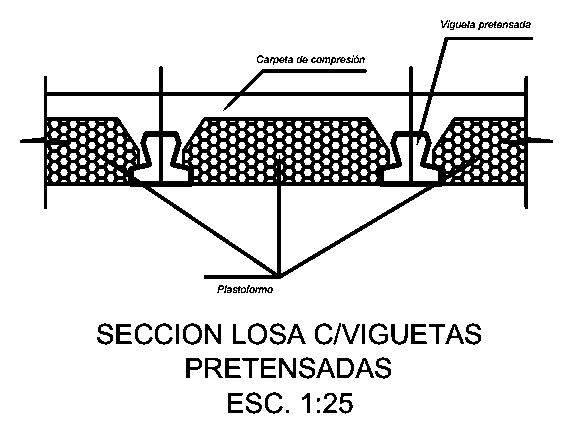
\includegraphics[width=0.60\linewidth]{plano02_seccion_losa_viguetas}
\nota{Tomado del Plano~02 del proyecto «Construcción Edificio de Posgrado» de la UATF.}
\end{figure}

Las especificaciones técnicas del proyecto exigen viguetas de hormigón de 350 a 400~kg/\cmdos{} y acero con una tensión de rotura de 18.000~kg/\cmdos{}, con superficie superior rugosa y certificación de IBNORCA e ISO; complementos de plastoformo de 100~$\times$~50~$\times$~20~cm; hormigón de 250~kg/\cmdos{} de resistencia característica, con al menos 400~kg/\mtres{} de cemento, vaciado de forma monolítica con las vigas; y parrilla de compresión y refuerzo de momentos negativos de fierro corrugado \parencite[p.~3]{uatf_et}. El certificado del fabricante de las viguetas indica ejes a 50~cm, un espesor de 20~+~5~=~25~cm, una sobrecarga admisible de 400~kg/\mdos{} y una luz máxima de 7,50~m simplemente apoyada, y exige una carpeta de al menos 21~MPa, aceros de continuidad y el cumplimiento de los pasos de montaje del fabricante \parencite{pretensa2025}. El proveedor de los complementos certificó 2.350 piezas de 20~$\times$~100~$\times$~44~cm y 10~kg/\mtres{} \parencite{unicon2025}, una medida distinta de la especificada. La Figura~\ref{fig:corte} muestra el corte transversal con la armadura de distribución de $\phi$6~c/20~cm en ambas direcciones.

\begin{figure}[H]
\centering
\caption{Corte transversal de la losa con la carpeta de compresión y la armadura de distribución}
\label{fig:corte}
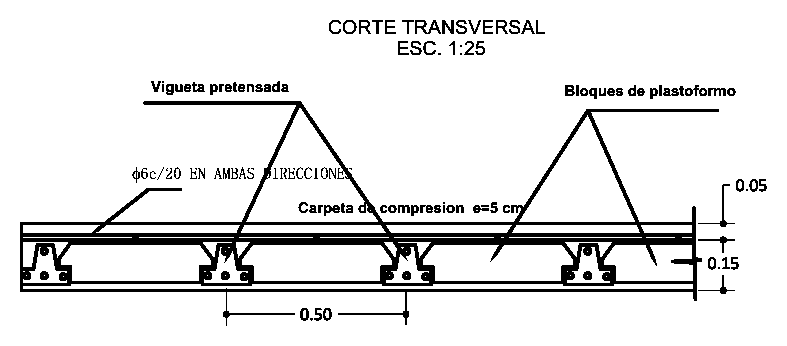
\includegraphics[width=0.85\linewidth]{plano02_corte_transversal}
\nota{Tomado del Plano~02 del proyecto. El corte acota 0,15~m de altura de complemento y 0,05~m de carpeta, mientras que las especificaciones técnicas y el certificado del fabricante indican 20~+~5~cm. Esta discrepancia se analiza en la sección~\ref{sec:analisis-documental}.}
\end{figure}

\subsection{Proceso constructivo y puntos críticos de calidad}

La ejecución sigue once actividades, desde la recepción de los materiales hasta el desapuntalamiento (Tabla~\ref{tab:proceso-losa}). En cada una hay un punto crítico: una característica que, si no se verifica en ese momento, no puede corregirse después sin retrabajo o desperdicio. El primero es la recepción, porque detectar un material defectuoso cuando ya está colocado obliga a retirarlo, detiene la obra y genera pérdidas de tiempo y de dinero \parencite[p.~115]{alcon2009}. El segundo es la liberación previa al vaciado, un punto de espera \parencite[anexo~4]{muro2020}: ningún elemento estructural debería vaciarse sin la autorización expresa de la Supervisión \parencite[p.~8]{ucb2025et}. El tercero es el hormigón, cuyo muestreo debe presenciar el supervisor \parencite[p.~37]{cajias2023}, con probetas elaboradas en el lugar de colocación y no a la salida de la hormigonera \parencite[p.~13]{ucb2025et}.

\begingroup\footnotesize\setstretch{1}\setlength{\tabcolsep}{4pt}
\begin{longtable}{@{}P{0.55cm}P{2.65cm}P{8.8cm}P{3.65cm}@{}}
\caption{Proceso constructivo de la losa alivianada y puntos críticos de calidad}\label{tab:proceso-losa}\\
\toprule
\textbf{N.\textsuperscript{o}} & \textbf{Actividad} & \textbf{Punto crítico de calidad} & \textbf{Criterio o referencia} \\
\midrule
\endfirsthead
\multicolumn{4}{@{}l}{\textit{(continuación)}}\\
\toprule
\textbf{N.\textsuperscript{o}} & \textbf{Actividad} & \textbf{Punto crítico de calidad} & \textbf{Criterio o referencia} \\
\midrule
\endhead
\bottomrule
\endfoot
1 & Recepción y acopio de viguetas & Cantidad, tipo y longitud según el plano de montaje del proveedor; piezas sin fisuras, oquedades ni armadura expuesta; tolerancias dimensionales & \textcite[pp.~115--116]{alcon2009}; NB~997:2016; certificado del fabricante \\
2 & Recepción y acopio de complementos & Dimensiones y densidad del pedido; piezas enteras; acopio protegido & Tolerancias de la ficha técnica; certificado del proveedor \\
3 & Recepción de cemento, áridos, agua y acero & Cemento con sello, bajo techo y en pilas de hasta 10 bolsas; agua limpia a más de 5~$^{\circ}$C; acero con certificado de fábrica, sin oxidación excesiva, barro ni aceite & ET, pp.~1--2; ACI~318-25, 26.6.1.2; pliego de referencia, p.~17 \\
4 & Replanteo y apuntalamiento & Puntales colocados antes de montar los complementos; niveles de apoyo según los planos & Ficha técnica de los complementos \\
5 & Colocación de viguetas & Separación de 50~cm entre ejes; tipo correcto en cada paño; empotramiento mínimo de 100~mm en vigas de borde y de 70~mm en vigas centrales & Certificado del fabricante; NBDS, art.~12 \\
6 & Colocación de complementos & Piezas enteras y bien asentadas; prohibido pisarlas & Ficha técnica de los complementos \\
7 & Nervios transversales y armaduras & Nervios rigidizadores según los planos; parrilla $\phi$6~c/20 en ambas direcciones; acero de continuidad sobre los apoyos; armadura apoyada dentro de las tolerancias & ET, p.~3; Plano~02; certificado del fabricante; ACI~318-25, 26.6.2 \\
8 & Instalaciones embebidas & Ductos y cajas fijados antes del vaciado sin desplazar la armadura & ACI~318-25, 26.13.3.3 \\
9 & Liberación para el vaciado & Punto de espera: verificación del armado, de las instalaciones y de la limpieza; mezcla aprobada para el elemento; autorización escrita de la Supervisión & ACI~318-25, 26.13.3.2 y 26.13.3.3; Supervisión \\
10 & Hormigonado & Vaciado monolítico con las vigas, por franjas y continuo hasta completar el paño; asentamiento controlado; compactación sin segregación; sin añadir agua más allá de lo que admite ASTM~C94; muestreo aleatorio & ET, p.~3; ACI~318-25, 26.5.2.2 y 26.12.2.1 \\
11 & Curado y desapuntalamiento & Humedad mantenida al menos 7 días con el hormigón a 10~$^{\circ}$C o más; protección en tiempo frío; puntales retirados solo cuando las probetas curadas en obra alcanzan la resistencia requerida & ACI~318-25, 26.5.3, 26.5.4 y 26.12.4 \\
\end{longtable}
\vspace{-6pt}
\nota{Elaboración propia con base en \textcite[pp.~115--116]{alcon2009}, las especificaciones técnicas del proyecto (ET) \parencite[pp.~1--3]{uatf_et}, el certificado del fabricante de las viguetas \parencite{pretensa2025}, las fichas técnicas \parencite[hoja~2]{concretec2018viguetas} \parencite[hojas~1 y 3]{concretec2016plastoformo}, la Norma Boliviana de Diseño Sísmico (NBDS) \parencite[p.~22]{mopsv2023nbds}, el código ACI~318-25 \parencite[secciones~26.5 a 26.13, pp.~578--611]{aci318_2025} y un pliego de especificaciones de referencia \parencite[pp.~8, 12--13, 17]{ucb2025et}.}
\endgroup

\subsection{Consumos teóricos de materiales por metro cuadrado}

Los consumos teóricos por metro cuadrado son la cantidad de referencia del índice de desperdicio (ecuación~\ref{eq:idm-marco}). Para una losa de viguetas simples con separación entre ejes $D$ y complementos de largo $L$, la geometría da directamente la longitud de vigueta por metro cuadrado, $1/D$, y el número de complementos, $1/(D \cdot L)$; el volumen mínimo de hormigón es el de la carpeta, $h_2 \times 1$~\mdos{}. Las fichas técnicas del fabricante dan la geometría del sistema, pero no tablas de consumo por metro cuadrado, por lo que estas cantidades son un cálculo propio sin descontar apoyos, bordes ni nervios transversales \parencite[hoja~3]{concretec2018viguetas}. \textcite[p.~103]{alcon2009} sí publicó consumos medidos para una losa de complemento de 15~cm, carpeta de 5~cm y ejes a 0,50~m: 2,00 piezas de complemento por metro cuadrado y 0,0666~\mtres{} de hormigón por metro cuadrado, valores promedio de diez mediciones. La Tabla~\ref{tab:consumos} compara ambas referencias.

\begingroup\small\setstretch{1}\setlength{\tabcolsep}{6pt}
\begin{longtable}{@{}P{3.3cm}P{3.4cm}P{3.4cm}P{5.1cm}@{}}
\caption{Consumos teóricos de referencia por metro cuadrado de losa}\label{tab:consumos}\\
\toprule
\textbf{Concepto} & \textbf{Alcón Aranda (2009): complemento de 15~cm, carpeta de 5~cm, $D = 0{,}50$~m} & \textbf{Geometría con $D = 0{,}50$~m y $L = 1{,}00$~m (cálculo propio)} & \textbf{Observación} \\
\midrule
\endfirsthead
\multicolumn{4}{@{}l}{\textit{(continuación)}}\\
\toprule
\textbf{Concepto} & \textbf{Alcón Aranda (2009): complemento de 15~cm, carpeta de 5~cm, $D = 0{,}50$~m} & \textbf{Geometría con $D = 0{,}50$~m y $L = 1{,}00$~m (cálculo propio)} & \textbf{Observación} \\
\midrule
\endhead
\bottomrule
\endfoot
Vigueta (m/\mdos{}) & 2,00 (35,00~kg/\mdos{} con 17,50~kg/m) & $1/D = 2{,}00$ & La longitud real depende de la luz de cada paño y de los apoyos \\
\addlinespace
Complementos (pza/\mdos{}) & 2,00 & $1/(D \cdot L) = 2{,}00$ & Piezas de 1,00~m de largo; se descuentan nervios y bordes \\
\addlinespace
Hormigón (\mtres{}/\mdos{}) & 0,0666 (333~\cmdos{} de sección por cada eje) & $\geq 0{,}05$ (solo la carpeta de 5~cm) & El volumen de los nervios depende de la sección de la vigueta y del perfil del complemento \\
\addlinespace
Peso propio (kg/\mdos{}) & 196,13 (hormigón 159,84; vigueta 35,00; complemento 1,29) & --- & Valor para la losa de 15~+~5~cm \\
\end{longtable}
\vspace{-6pt}
\nota{Elaborado con base en \textcite[p.~103]{alcon2009} y en la geometría de las fichas técnicas \parencite[hoja~3]{concretec2018viguetas}. Los valores de la tercera columna son cálculo propio, sin desperdicio y sin descontar apoyos, bordes ni nervios transversales.}
\endgroup

Para la losa del Edificio de Posgrado, con ejes a 0,50~m y piezas de 1,00~m de largo, la geometría da 2,00 complementos por metro cuadrado, es decir, unas 2.220 piezas teóricas brutas para los 1.109,84~\mdos{} de la primera losa (cálculo propio), frente a las 2.350 piezas certificadas por el proveedor \parencite{unicon2025}: una diferencia preliminar de unas 130 piezas ($\approx$~6~\%) antes de descontar nervios y bordes. En el acero, el cómputo de la planilla N.\textsuperscript{o}~2 asigna a la losa 4.171,18~kg \parencite[pp.~19--20]{uatf2025pao2}, equivalentes a 3,76~kg/\mdos{} (cálculo propio). Ambas cifras son preliminares: el capítulo~2 las precisa con el Plano~03 y las concilia con los demás documentos de la obra (sección~\ref{sec:analisis-documental}).

\subsection{Defectos frecuentes y su prevención}

Los defectos de la losa tienen tres orígenes: el producto prefabricado, el montaje y el hormigonado. En las viguetas, \textcite[p.~116]{alcon2009} distingue los defectos leves, que no implican riesgo estructural pero dificultan el montaje y cuya aceptación queda a criterio del supervisor, de los graves, que implican riesgo para la estructura o impiden el montaje y obligan a devolver el material al proveedor. La NB~997, en la versión que recoge \textcite[pp.~89--92]{capcha2016}, exige viguetas sin discontinuidades de hormigonado visibles, oquedades, armaduras expuestas ni fisuras, y rechaza el lote cuando los defectos principales o secundarios superan los límites; esa versión es anterior a la NB~997:2016, con la que debe contrastarse. En el hormigonado, los defectos más frecuentes son la segregación y las cangrejeras, que representaron el 42,7~\% de las no conformidades en la estructura estudiada por \textcite[pp.~16--17]{muro2020}; el vibrado fue la actividad con más no conformidades en la obra estudiada por \textcite[p.~86]{ferrer2018}, por falta de capacitación, ausencia del encargado y equipos inadecuados. La Tabla~\ref{tab:defectos} resume los defectos frecuentes de la losa, sus causas y su prevención.

\begingroup\footnotesize\setstretch{1}\setlength{\tabcolsep}{4pt}
\begin{longtable}{@{}P{3.2cm}P{3.6cm}P{6.2cm}P{2.6cm}@{}}
\caption{Defectos frecuentes de la losa alivianada, causas y prevención}\label{tab:defectos}\\
\toprule
\textbf{Defecto} & \textbf{Causa probable} & \textbf{Prevención y control} & \textbf{Referencia} \\
\midrule
\endfirsthead
\multicolumn{4}{@{}l}{\textit{(continuación)}}\\
\toprule
\textbf{Defecto} & \textbf{Causa probable} & \textbf{Prevención y control} & \textbf{Referencia} \\
\midrule
\endhead
\bottomrule
\endfoot
Viguetas fisuradas, rotas o con armadura expuesta & Fabricación deficiente; golpes en el transporte, la descarga o el montaje & Inspección en la descarga; devolución de las piezas con defectos graves & \textcite[p.~116]{alcon2009}; NB~997 \\
Vigueta de tipo o longitud equivocados & Pedido sin el plano de montaje del proveedor & Verificar tipo y cantidad contra el plano de montaje & \textcite[p.~116]{alcon2009} \\
Deformación o caída de la losa durante el montaje & Complementos colocados sobre viguetas sin apuntalar & Apuntalar las viguetas antes de colocar los complementos & \textcite[hoja~3]{concretec2016plastoformo} \\
Mayor consumo de hormigón en la carpeta & Complementos pisados y deformados & No pisar las piezas colocadas & \textcite[hoja~3]{concretec2016plastoformo} \\
Segregación y cangrejeras & Vibrado deficiente; incumplimiento del procedimiento de vaciado; personal sin capacitación & Procedimiento de vaciado y vibrado; capacitación; inspección continua del vaciado & \textcite[pp.~16--17]{muro2020}; ACI~318-25, 26.5.2.2 \\
Juntas frías & Interrupciones del vaciado & Vaciado continuo hasta completar el paño o una junta prevista; vaciado por franjas & ACI~318-25, 26.5.2.2; ET, p.~3 \\
Armadura desplazada o con recubrimiento insuficiente & Falta de apoyos o separadores; tránsito sobre la armadura & Apoyar la armadura para que no se desplace durante el vaciado; verificar tolerancias & ACI~318-25, 26.6.2 \\
Falta de continuidad sobre los apoyos & Omisión del acero de continuidad o de los negativos & Verificar el acero sobre los apoyos antes de liberar el paño & Certificado del fabricante; NBDS, art.~12 \\
Resistencia insuficiente del hormigón & Dosificación sin aprobar; agua añadida; curado insuficiente; tiempo frío & Dosificación aprobada; no añadir agua más allá de lo que admite ASTM~C94; curado de 7 días; plan de tiempo frío; aceptación con ensayos & ACI~318-25, 26.4.4, 26.5.2.2, 26.5.3, 26.5.4 y 26.12.3 \\
Fisuras y flechas excesivas & Desapuntalamiento prematuro & Retirar los puntales solo con probetas curadas en obra que alcancen la resistencia requerida & ACI~318-25, 26.12.4 \\
\end{longtable}
\vspace{-6pt}
\nota{Elaboración propia con base en las fuentes indicadas: \textcite[p.~116]{alcon2009}, \textcite[hoja~3]{concretec2016plastoformo}, \textcite[pp.~16--17]{muro2020}, el código ACI~318-25 \parencite[secciones~26.4 a 26.12, pp.~577--604]{aci318_2025}, las especificaciones técnicas del proyecto (ET) \parencite[p.~3]{uatf_et}, el certificado del fabricante \parencite{pretensa2025} y la NBDS \parencite[p.~22]{mopsv2023nbds}.}
\endgroup

% ---------------------------------------------------------------------
\section{Marco normativo}
\label{sec:marco-normativo}

El SGC de la losa se apoya en las normas de gestión de la calidad, que definen la estructura del sistema; en las normas técnicas, que fijan los requisitos de los materiales, de la ejecución y de los ensayos; y en la legislación de contratación pública, que define los roles, los documentos y las reglas económicas del contrato (Tabla~\ref{tab:marco-normativo}).

\subsection{Normas de gestión de la calidad}

Las normas ISO~9000:2026 (fundamentos y vocabulario), ISO~9001:2026 (requisitos del SGC), ISO~10005:2018 (planes de la calidad) e ISO~10006:2017 (gestión de la calidad en proyectos) se describieron en la sección~\ref{sec:sgc-iso}. Su aplicación es voluntaria, pero se vuelve obligatoria cuando se incorpora a los documentos del contrato: las especificaciones técnicas forman parte del documento base de contratación, las elabora la entidad contratante y fijan las características técnicas de la obra \parencite[art.~5, inc.~m, p.~21]{ds0181_2025compilado}. Por eso, el plan de la calidad y el plan de puntos de inspección de la losa deben incluirse en las especificaciones del documento de contratación del saldo de la obra.

\subsection{Normas técnicas del hormigón, de las viguetas y de los ensayos}

Las especificaciones técnicas del proyecto exigen que los hormigones y la losa cumplan la Norma Boliviana del Hormigón Armado CBH-87 y normas bolivianas de cemento, áridos y agua de ediciones antiguas \parencite[pp.~1--3]{uatf_et}. La norma técnica boliviana actual de hormigón estructural es la NB~1225001-1:2017 \parencite{nb1225001_2017}, basada en el código ACI~318 \parencite[p.~4]{cocarico2022}. La Norma Boliviana de Diseño Sísmico (NBDS) remite a ella como norma de diseño específica para el hormigón estructural y dispone que ambas se apliquen en conjunto, con prevalencia de la norma sísmica en caso de contradicción \parencite[arts.~1 y 10, pp.~1, 19]{mopsv2023nbds}; no menciona la CBH-87. La R.~M.~271/2023 del Ministerio de Obras Públicas, Servicios y Vivienda, que aprueba la NBDS, la declara de aplicación obligatoria en todo el país \parencite[R.~M.~271/2023, resuelve tercero]{mopsv2023nbds}, pero en los documentos del repositorio no consta un instrumento que declare obligatorias la NB~1225001 o la CBH-87. Por eso, esta tesis trata la CBH-87 como la norma que cita la especificación técnica del ítem y toma como marco técnico vigente la NBDS y la NB~1225001. \pendiente{verificar si existen instrumentos legales vigentes que declaren obligatorias la CBH-87 (la bibliografía recomendada menciona el D.~S.~22976 de 1991) y la NB~1225001 (R.~M. del MOPSV 172/2020); ninguno de ellos está en el repositorio}

Como el texto de la NB~1225001 no está disponible en el repositorio y esa norma se basa en el código ACI~318, esta tesis adopta como referencia técnica para el control y la aceptación del hormigón el capítulo~26 del ACI~CODE-318-25, sin atribuirle la numeración de la norma boliviana. Un ensayo de resistencia es el promedio de al menos dos cilindros de la misma muestra, tomada en el punto de entrega según ASTM~C172, curados según ASTM~C31 y ensayados según ASTM~C39 a los 28 días \parencite[sección~26.12.1.1, p.~601]{aci318_2025}. Se toma al menos una muestra por día, por cada 150~yd\textsuperscript{3} ($\approx$~114,7~\mtres{}) y, en losas, por cada 5.000~ft\textsuperscript{2} ($\approx$~464,5~\mdos{}) de superficie; si esa frecuencia diera menos de cinco ensayos para una mezcla, las probetas se elaboran de al menos cinco pastones elegidos al azar \parencite[sección~26.12.2.1, p.~603]{aci318_2025}. Para los 1.109,84~\mdos{} de la primera losa, el criterio de superficie exige al menos tres muestras (cálculo propio). La resistencia se acepta si todo promedio de tres ensayos consecutivos iguala o supera $f'_c$ y ningún ensayo queda por debajo de $f'_c$ en más de 500~psi cuando $f'_c \leq 5.000$~psi \parencite[sección~26.12.3.1, p.~603]{aci318_2025}; para el H25 de la losa, ningún ensayo puede ser menor de unos 214,8~kg/\cmdos{} (cálculo propio). Ante resultados bajos se extraen tres núcleos por ensayo deficiente, y el hormigón es adecuado si su promedio alcanza el 85~\% de $f'_c$ y ningún núcleo baja del 75~\% \parencite[sección~26.12.7, p.~606]{aci318_2025}. El código exige además mantener la humedad del hormigón durante 7 días a 10~$^{\circ}$C o más \parencite[sección~26.5.3.2, p.~581]{aci318_2025}, presentar un plan de hormigonado en tiempo frío \parencite[sección~26.5.4.2, p.~583]{aci318_2025} e inspeccionar la conformidad con los documentos de construcción en todas las etapas, con registros conservados al menos dos años \parencite[secciones~26.13.1.2 y 26.13.2.1, pp.~608, 610]{aci318_2025}.

Para las losas de viguetas prefabricadas que deben funcionar como diafragma rígido, la norma sísmica exige una altura mínima de 250~mm con la carpeta, una carpeta de al menos 50~mm con malla de 6~mm cada 250~mm, el empotramiento de las viguetas en las vigas, nervios rigidizadores a no más de 2,50~m, una separación entre ejes no mayor que el doble de la altura y el hormigonado simultáneo de la losa con sus vigas de apoyo \parencite[art.~12, p.~22]{mopsv2023nbds}; además, fija una resistencia mínima del hormigón de 21~MPa y recomienda 25~MPa \parencite[art.~16, p.~28]{mopsv2023nbds}. La especificación de la obra (20~+~5~cm, ejes a 50~cm, parrilla $\phi$6~c/20 y vaciado monolítico con las vigas) es coherente con esos mínimos, no así el corte del Plano~02, que acota una altura total de 0,20~m (Figura~\ref{fig:corte}); la discrepancia debe resolverla la Supervisión con el proyectista.

Las viguetas se rigen por la NB~997:2016, que establece sus requisitos y métodos de ensayo \parencite{nb997_2016} y cuyo cumplimiento declara el certificado del fabricante de la obra \parencite{pretensa2025}. Los ensayos se basan en normas ASTM, como pide la guía del docente \parencite[diapositiva~25]{barrios2021documento}: C172, C31 y C39 para el muestreo, las probetas y la resistencia; C143 para el asentamiento; y A615 para las barras corrugadas, que el código ACI admite como refuerzo \parencite[sección~20.2.1.3, p.~409]{aci318_2025}.

\subsection{Legislación de contratación pública}

La Ley~1178 de Administración y Control Gubernamentales crea el Sistema de Administración de Bienes y Servicios, que debe identificar a los responsables de las decisiones de contratación en relación con la calidad, la oportunidad y el precio de lo contratado \parencite[art.~10]{ley1178_1990}. La misma ley establece el control interno previo, que se aplica antes de que las operaciones surtan efecto \parencite[arts.~13--14]{ley1178_1990}, lógica equivalente a la de los puntos de espera de un plan de inspección. Sus normas básicas, el D.~S.~0181 (NB-SABS), regulan las modificaciones de los contratos de obra \parencite[art.~89, pp.~91--93]{ds0181_2025compilado}:
\begin{itemize}
  \item el \textbf{contrato modificatorio} procede cuando cambian el alcance, el monto o el plazo sin aumentar los precios unitarios; uno o varios, sumados, no pueden superar el 10~\% del monto del contrato principal, y los precios de los ítems nuevos se negocian;
  \item la \textbf{orden de cambio}, exclusiva de obras, modifica el precio o el plazo sin aumentar los precios unitarios ni crear ítems nuevos, y no puede superar el 5~\%;
  \item en licitación pública, ambos instrumentos sumados no pueden exceder el 15~\% del monto del contrato principal.
\end{itemize}
Las mismas normas establecen la recepción provisional y definitiva de las obras \parencite[art.~39, p.~54]{ds0181_2025compilado}. Los modelos de documento base de contratación de obras vigentes fueron aprobados por la R.~M.~048/2024 del Ministerio de Economía y Finanzas Públicas, que sustituyó a los de 2022 \parencite{rm048_2024}. El modelo de 2022, disponible en el repositorio, define las figuras contractuales que el SGC debe operar: el Libro de Órdenes, en el que el Supervisor anota sus instrucciones \parencite[cláusula~25, p.~71]{dbc2022}; la responsabilidad de la Supervisión sobre el control de calidad y los ensayos a cargo del contratista \parencite[cláusulas~26.3 y 26.6, p.~73]{dbc2022}; y la prohibición de cubrir un trabajo sin aprobación previa \parencite[cláusula~26.10, p.~74]{dbc2022}. Esas cláusulas deben contrastarse con el contrato real de la obra.

Frente al alza de precios de 2025 y 2026 se dictaron decretos de ajuste excepcional. El D.~S.~5321 permitió ajustar, mediante un contrato modificatorio, el precio de los materiales importados de su anexo ---entre ellos el acero corrugado---, considerando solo el componente de materiales del análisis de precios unitarios y aun por encima de los porcentajes del art.~89 \parencite[arts.~3--4 y anexo]{ds5321_2025}; los D.~S.~5406 y 5452 ampliaron su plazo y fijaron la fórmula del ajuste \parencite{ds5406_2025,ds5452_2025}. El D.~S.~5597 extendió el ajuste a todos los materiales, maquinaria y equipo hasta el 31 de diciembre de 2026 y previó la resolución del contrato por una situación ajena a las partes cuando el incremento de precios no sea viable, inviabilidad que puede considerarse caso fortuito y que no da lugar a registrar al contratista como impedido en el Sistema de Contrataciones Estatales (SICOES) ni a ejecutar su garantía de cumplimiento \parencite[art.~4 y disposición adicional quinta]{ds5597_2026}. Las NB-SABS definen la fuerza mayor como un obstáculo externo, imprevisto o inevitable, ajeno al hombre, como un incendio, una inundación u otro desastre natural, y el caso fortuito como un obstáculo interno atribuible al hombre, imprevisto o inevitable, como una conmoción civil, una huelga o un bloqueo \parencite[art.~5, incs.~c y p, pp.~20, 22]{ds0181_2025compilado}. En la obra estudiada, el contrato excluía el reajuste de precios \parencite[p.~95]{uatf2025pao2}, el contrato modificatorio (+7,22~\%) quedó dentro del límite del 10~\% (Tabla~\ref{tab:datos-contractuales}) y la solicitud de resolución del contratista (5 de enero de 2026), que invocó la fuerza mayor o el caso fortuito \parencite[p.~14]{uatf_item13}, es anterior al D.~S.~5597, cuya aplicabilidad al caso corresponde valorar a la asesoría legal de la entidad. Para aislar el efecto del SGC de estas variaciones, la evaluación de la tesis se hace a precios constantes del contrato.

\begingroup\footnotesize\setstretch{1}\setlength{\tabcolsep}{3pt}
\begin{longtable}{@{}P{3.0cm}P{4.0cm}P{5.1cm}P{3.5cm}@{}}
\caption{Marco normativo del SGC de la losa alivianada}\label{tab:marco-normativo}\\
\toprule
\textbf{Norma o instrumento} & \textbf{Objeto} & \textbf{Aplicación en esta tesis} & \textbf{Fuente} \\
\midrule
\endfirsthead
\multicolumn{4}{@{}l}{\textit{(continuación)}}\\
\toprule
\textbf{Norma o instrumento} & \textbf{Objeto} & \textbf{Aplicación en esta tesis} & \textbf{Fuente} \\
\midrule
\endhead
\bottomrule
\endfoot
\multicolumn{4}{@{}l}{\textit{Gestión de la calidad}}\\*
ISO~9000:2026 & Fundamentos, principios y vocabulario & Definiciones de calidad, requisito, no conformidad y acción correctiva & \textcite{iso9000_2026} \\
ISO~9001:2026; NB/ISO~9001:2026 & Requisitos de un SGC (cláusulas 4 a 10) & Estructura del SGC propuesto & \textcite{iso9001_2026}; \textcite{ibnorca9001_2026} \\
ISO~10005:2018 & Directrices para los planes de la calidad & Plan de la calidad de la losa & \textcite{iso10005_2018} \\
ISO~10006:2017 & Directrices para la gestión de la calidad en los proyectos & Responsabilidades de las organizaciones del proyecto y control de los cambios & \textcite{iso10006_2017} \\
\multicolumn{4}{@{}l}{\textit{Normas técnicas}}\\*
CBH-87 & Norma boliviana de hormigón armado citada en las especificaciones del proyecto & Requisitos contractuales de materiales y ejecución & \textcite[pp.~1--3]{uatf_et} \\
NB~1225001-1:2017 & Hormigón estructural, basada en el código ACI~318 & Norma técnica boliviana de referencia, a la que remite la NBDS & \textcite{nb1225001_2017}; \textcite[p.~4]{cocarico2022}; \textcite[arts.~1 y 10]{mopsv2023nbds} \\
ACI~CODE-318-25, capítulo~26 & Producción, colocación, curado, evaluación, aceptación e inspección del hormigón & Muestreo (26.12.2.1), aceptación (26.12.3.1), curado (26.5.3), tiempo frío (26.5.4), armaduras (26.6) e inspección (26.13) & \textcite{aci318_2025} \\
NBDS 2023 (R.~M.~271/2023), art.~12 & Norma sísmica de aplicación obligatoria; losas de viguetas prefabricadas como diafragma rígido & Verificación de la altura, la carpeta, los apoyos y el hormigonado de la losa & \textcite[resuelve tercero; art.~12, p.~22]{mopsv2023nbds} \\
NB~997:2016 & Viguetas prefabricadas de hormigón pretensado: requisitos y métodos de ensayo & Recepción y liberación de viguetas por lote & \textcite{nb997_2016}; \textcite{pretensa2025} \\
ASTM~C172, C31 y C39 & Muestreo del hormigón fresco, elaboración y curado de probetas, y ensayo de compresión & Plan de muestreo y ensayos de aceptación del hormigón & \textcite[sección~26.12.1.1, p.~601]{aci318_2025} \\
ASTM~C143 & Asentamiento del hormigón fresco con el cono de Abrams & Control de la consistencia de cada pastón muestreado & \textcite[diapositiva~25]{barrios2021documento}; \textcite[p.~9]{ucb2025et} \\
ASTM~A615 & Barras corrugadas de acero al carbono & Recepción del acero con certificado de fábrica & \textcite[secciones~20.2.1.3 y 26.6.1.2, pp.~409, 587]{aci318_2025} \\
\multicolumn{4}{@{}l}{\textit{Legislación de contratación pública}}\\*
Ley~1178 (SAFCO) & Administración y control gubernamentales & Responsabilidad por la calidad de lo contratado; control interno previo & \textcite[arts.~10, 13 y 14]{ley1178_1990} \\
D.~S.~0181 (NB-SABS) & Normas básicas de contratación de bienes, obras y servicios & Contrato modificatorio $\leq$ 10~\%; orden de cambio $\leq$ 5~\%; ambos $\leq$ 15~\% en licitación pública (art.~89); recepción provisional y definitiva (art.~39) & \textcite[pp.~54, 91--93]{ds0181_2025compilado} \\
R.~M.~048/2024; modelo de DBC de 2022 (sustituido) & Modelos de documento base de contratación de obras & Supervisor y Fiscal, Libro de Órdenes, ensayos a cargo del contratista, medición neta y planillas & \textcite{rm048_2024}; \textcite[pp.~71--75]{dbc2022} \\
D.~S.~5321, 5406 y 5452 (2025) & Ajuste excepcional de precios de materiales importados & Contexto de precios; el modelo de la tesis usa precios constantes & \textcite{ds5321_2025}; \textcite{ds5406_2025}; \textcite{ds5452_2025} \\
D.~S.~5597 (2026) & Ajuste excepcional de precios de materiales, maquinaria y equipo; resolución por situación ajena a las partes & Contexto de la paralización y de la contratación del saldo de la obra & \textcite{ds5597_2026} \\
\end{longtable}
\vspace{-6pt}
\nota{Elaborado con base en las fuentes citadas. DBC: documento base de contratación; NBDS: Norma Boliviana de Diseño Sísmico; NB-SABS: Normas Básicas del Sistema de Administración de Bienes y Servicios.}
\endgroup

% ---------------------------------------------------------------------
\section{Control de costos en obras públicas}
\label{sec:control-costos}

\subsection{Análisis de precios unitarios}

En las obras públicas bolivianas, el costo de cada ítem se expresa en un análisis de precios unitarios (APU) con el formulario B-2 del modelo de documento base de contratación \parencite[p.~257]{cocarico2022}, que suma a los costos directos ---materiales, mano de obra y equipo--- las incidencias de beneficios sociales, herramientas, gastos generales, utilidad e impuestos \parencite[p.~254]{cocarico2022}. Como cada incidencia se aplica sobre una base distinta \parencite[pp.~256--257]{cocarico2022}, el precio unitario resulta
\begin{equation}
  PU = \underbrace{\left[M + MO\,(1+b)(1+i_v)(1+h) + E\right]}_{CD}\,(1+g)\,(1+u)\,(1+t)
  \label{eq:apu}
\end{equation}
donde $M$ es el costo de los materiales, $MO$ el de la mano de obra, $E$ el del equipo y la maquinaria, $CD$ el costo directo, y $b$, $i_v$, $h$, $g$, $u$ y $t$ las incidencias de beneficios sociales, impuesto al valor agregado, herramientas, gastos generales, utilidad e impuesto a las transacciones. En un APU boliviano documentado se adoptaron $b = 71~\%$, $h = 5~\%$, $g = 13~\%$, $u = 10~\%$, $i_v = 14{,}94~\%$ y $t = 3{,}09~\%$ \parencite[p.~256]{cocarico2022}. Con esos valores, cada boliviano de costo directo se convierte en unos 1,28 bolivianos de precio unitario (cálculo propio: $1{,}13 \times 1{,}10 \times 1{,}0309 \approx 1{,}281$). La ecuación muestra también que el desperdicio de materiales no solo aumenta $M$: arrastra los gastos generales, la utilidad y los impuestos calculados sobre él.

El efecto económico del desperdicio depende de quién lo absorbe. El porcentaje de pérdidas que el proponente incluye en las cantidades de su APU lo paga la entidad dentro del precio unitario; el desperdicio que excede ese porcentaje y el retrabajo los absorbe el contratista, porque el precio unitario es fijo. Si los costos de producción suben de forma imprevista, el constructor solo puede trasladarlos al cliente o reducir su margen \parencite[p.~24]{pons2014}; en un contrato público sin reajuste de precios, como el de la obra estudiada \parencite[p.~95]{uatf2025pao2}, solo queda la segunda opción. Para la entidad, en cambio, el riesgo es pagar cantidades no ejecutadas o mal medidas.

\subsection{Cómputos métricos, planillas de avance y modificaciones}

Los cómputos métricos determinan las cantidades de cada ítem a partir de los planos, por elemento y por nivel \parencite[p.~254]{cocarico2022}. Su criterio de medición debe estar definido de antemano: un pliego de especificaciones de referencia mide las losas con viguetas prefabricadas por metro cuadrado entre ejes de las vigas, y el volumen de hormigón como un ítem distinto \parencite[p.~19]{ucb2025et}, mientras que en la obra estudiada el ítem de la losa se paga por metro cuadrado \parencite[p.~16]{uatf2025pao2} e incluye el hormigón \parencite[p.~3]{uatf_et}. El cómputo de la cantidad teórica es, además, la referencia del índice de desperdicio (ecuación~\ref{eq:idm-marco}).

El pago sigue el avance de la obra: el contratista presenta cada mes una planilla o certificado de pago, que el Supervisor revisa y aprueba \parencite[cláusula~28, p.~75]{dbc2022} después de medir la obra junto con el contratista \parencite[cláusula~26.3, p.~72]{dbc2022}. Las obras se miden netas, sin pagar volúmenes excedentes no aprobados por escrito \parencite[cláusula~27, p.~75]{dbc2022}, y la planilla de cantidades finales debe basarse en la obra realmente ejecutada \parencite[cláusula~38.1, p.~86]{dbc2022}; el Supervisor certifica los volúmenes y la calidad de los ítems ejecutados \parencite[p.~14]{cajias2023}.

Los cambios de cantidades se formalizan con tres instrumentos. La orden de trabajo redistribuye cantidades sin cambiar el precio ni el plazo y sin crear ítems \parencite[p.~20]{dbc2022}; la orden de cambio y el contrato modificatorio modifican el precio, el plazo o el alcance dentro de los límites del art.~89 de las NB-SABS (sección~\ref{sec:marco-normativo}). Todos deben emitirse antes de ejecutar los trabajos y no sirven para regularizar lo ya ejecutado \parencite[cláusula~30.5, p.~78]{dbc2022}. En el reajuste excepcional de precios, la variación de cada material es la diferencia entre su precio actual y el precio inicial del contrato, y el monto del ajuste es la suma de esas variaciones multiplicadas por las cantidades pendientes \parencite[art.~2]{ds5452_2025}.

Desde la gestión de la calidad, estos instrumentos tienen dos lecturas. La conciliación entre el cómputo teórico, la cantidad consumida y la cantidad pagada es un control de la calidad de la información, porque una diferencia no explicada revela desperdicio, sobremedición o un error de cómputo. Y las sobremediciones corregidas en planillas posteriores son fallas externas en el sentido del modelo PEF: se detectan después de que el producto ---la planilla--- fue entregado al cliente.

% ---------------------------------------------------------------------
\section{Herramientas de la calidad}
\label{sec:herramientas}

Según la clasificación que recoge \textcite[p.~26]{zurita2024}, las herramientas básicas de la calidad son siete: la hoja de recogida de datos, el histograma, el diagrama de Pareto, el diagrama de causa y efecto, la estratificación, el diagrama de dispersión y el gráfico de control, a las que se suma el diagrama de flujo. Su valor está en su uso encadenado: la hoja de verificación produce los datos, el diagrama de Pareto prioriza los problemas, el diagrama de Ishikawa busca sus causas, y el histograma y la carta de control muestran si el proceso mejora. A ellas se agregan el plan de puntos de inspección, que organiza los controles de la obra, y la técnica 5W2H, que estructura las acciones de mejora (Tabla~\ref{tab:herramientas}).

\begingroup\footnotesize\setstretch{1}\setlength{\tabcolsep}{4pt}
\begin{longtable}{@{}P{2.4cm}P{4.9cm}P{5.4cm}P{2.9cm}@{}}
\caption{Herramientas de la calidad y su uso en esta tesis}\label{tab:herramientas}\\
\toprule
\textbf{Herramienta} & \textbf{Para qué sirve} & \textbf{Uso en esta tesis} & \textbf{Fuente} \\
\midrule
\endfirsthead
\multicolumn{4}{@{}l}{\textit{(continuación)}}\\
\toprule
\textbf{Herramienta} & \textbf{Para qué sirve} & \textbf{Uso en esta tesis} & \textbf{Fuente} \\
\midrule
\endhead
\bottomrule
\endfoot
Hoja de verificación & Registrar datos de forma ordenada para distinguir hechos de opiniones y comprobar la repetición de un problema o defecto & Fichas de recepción de materiales, de consumo por paño y de inspección del PPI; lista de verificación de los requisitos de la ISO~9001 & \textcite[p.~27]{gudiel2020} \\
\addlinespace
Diagrama de Pareto & Ordenar las causas o los defectos de mayor a menor frecuencia o costo para atender primero los pocos que explican la mayor parte del problema (regla 80/20) & Priorizar las no conformidades y las pérdidas de la línea base por su costo; elegir las partidas de control & \textcite[pp.~32--35]{gudiel2020}; \textcite[p.~70]{alfaro2011} \\
\addlinespace
Diagrama de Ishikawa & Representar las posibles causas de un problema agrupadas por categorías (materiales, personal, métodos, maquinaria) & Analizar las causas del desperdicio y de las no conformidades de la primera losa & \textcite[pp.~29--31]{gudiel2020} \\
\addlinespace
Histograma & Mostrar la distribución, la dispersión y la tendencia de un conjunto de mediciones & Distribución de las resistencias del hormigón y de la reducción del costo simulada & \textcite[pp.~36--38]{gudiel2020} \\
\addlinespace
Carta de control & Seguir en el tiempo la variabilidad de un proceso y distinguir las causas comunes de las especiales & Seguimiento del índice de desperdicio por vaciado y de las resistencias por losa & \textcite[pp.~11--12]{aguilar2016}; \textcite[p.~331]{formoso1999} \\
\addlinespace
Plan de puntos de inspección (PPI) & Definir para cada inspección el criterio de aprobación, el lote, la frecuencia, el responsable y los puntos de parada & PPI de la losa, con puntos de espera antes del vaciado y en la recepción de materiales (capítulo~2) & \textcite[anexo~4]{muro2020}; \textcite[p.~64]{ferrer2018} \\
\addlinespace
5W2H & Planificar una acción respondiendo qué, por qué, dónde, cuándo, quién, cómo y cuánto cuesta & Planes de acción correctiva de las no conformidades y del plan de implantación del SGC & Técnica de uso general \\
\end{longtable}
\vspace{-6pt}
\nota{Elaborado con base en las fuentes citadas; la columna de uso es de elaboración propia.}
\endgroup

En esta tesis, la hoja de verificación es la base de los registros del SGC: sin ella no hay datos para calcular el índice de desperdicio ni el costo de no calidad. El diagrama de Ishikawa ordena las causas de las pérdidas de la losa en las categorías de \textcite[pp.~12--13]{luangcharoenrat2019}, y el histograma y la carta de control se aplican a las resistencias del hormigón, cuya variabilidad fundamenta los criterios estadísticos de aceptación \parencite[p.~58]{alcon2009}, y a los índices de desperdicio de cada vaciado, para distinguir una variación normal de una causa especial que exige acción \parencite[p.~27]{cepeda2017}. La técnica 5W2H asegura que cada acción correctiva tenga responsable, plazo y costo, de modo que la mejora pueda verificarse.

% ---------------------------------------------------------------------
\section{Evaluación \emph{ex ante} y simulación}
\label{sec:simulacion-marco}

\subsection{Modelo de simulación teórica con tratamiento de control}

La guía del docente reconoce cuatro tipos de modelo de investigación: el desarrollo teórico, la modelación teórica, la modelación experimental y la modelación de simulación teórica \parencite[diapositiva~4]{barrios2021modelo}. Todo modelo debe incluir un tratamiento de control que sirva de comparación, generalmente un no tratamiento \parencite[diapositiva~8]{barrios2021modelo}, y debe permitir calcular el grado de incertidumbre, es decir, la probabilidad de obtener los resultados observados solo por efecto del azar \parencite[diapositiva~9]{barrios2021modelo}. Su estructura avanza de la conceptualización y el alcance a la definición de factores y variables, el procedimiento y la toma de observaciones, la validación de las observaciones y el contraste de hipótesis y resultados \parencite[diapositiva~12]{barrios2021modelo}, secuencia que sigue el capítulo~2. En términos experimentales, la esencia de un experimento es la manipulación intencional de una acción para analizar sus posibles resultados \parencite[p.~151]{hernandez2018}, y el grupo de control es el que no recibe el tratamiento \parencite[p.~154]{hernandez2018}.

Cuando el tratamiento no puede aplicarse en el objeto real, como ocurre con un SGC cuya obra se paralizó, la comparación se hace sobre un modelo. Una evaluación \emph{ex ante} estima el efecto de una intervención antes de aplicarla: el sistema se representa con un modelo de costos, se simula sin SGC (control) y con SGC (tratamiento), y la diferencia se atribuye al tratamiento tal como el modelo lo representa. Su validez depende de que los supuestos y los parámetros sean explícitos, trazables y verificables, exigencia que no cumplen todos los antecedentes: \textcite[p.~148]{chino2024} proyectaron un método de control del acero sobre niveles ya construidos con el método convencional, y \textcite[pp.~23--24, 51--52]{delavega2023} simularon patrones de corte del acero sin informar el desperdicio de la línea base, lo que impide cuantificar la reducción.

\subsection{Método de Monte Carlo}

Sea $Y = g(X_1, \dots, X_k)$ una variable de salida cuyas entradas $X_j$ son inciertas y se representan con distribuciones de probabilidad; el método de Monte Carlo estima la distribución de $Y$ por muestreo aleatorio. Consta de cinco pasos: formular el modelo determinista $g$; asignar a cada entrada incierta una distribución; generar $N$ juegos de valores aleatorios de las entradas; calcular $Y$ para cada juego; y analizar la muestra $\{Y_1, \dots, Y_N\}$ mediante su media, su desviación estándar, sus percentiles y las probabilidades de interés. La media y una probabilidad se estiman, con sus errores estándar, como
\begin{equation}
  \bar{Y}_N = \frac{1}{N}\sum_{k=1}^{N} Y_k, \qquad EE\!\left(\bar{Y}_N\right) = \frac{s_Y}{\sqrt{N}}, \qquad
  \hat{p} = \frac{1}{N}\sum_{k=1}^{N} \mathbf{1}\!\left(r_k \geq r^{*}\right), \qquad EE\!\left(\hat{p}\right) = \sqrt{\frac{\hat{p}\,(1-\hat{p})}{N}}
  \label{eq:montecarlo}
\end{equation}
donde $s_Y$ es la desviación estándar de la muestra simulada, $\mathbf{1}(\cdot)$ vale 1 si se cumple la condición y 0 si no, $r_k$ es la reducción relativa del costo unitario en la iteración $k$ y $r^{*}$ el umbral de la hipótesis. En un modelo con tratamiento de control, en cada iteración se calculan ambas condiciones con el mismo juego de parámetros de la línea base, de modo que su diferencia solo refleja el efecto del tratamiento. La proporción de iteraciones en que la reducción alcanza el umbral es la probabilidad de cumplir la hipótesis, que expresa el grado de incertidumbre que pide la guía del docente. Una regla de decisión de la forma $\hat{P}(r \geq r^{*}) \geq 0{,}95$ equivale a exigir que el percentil 5 de la reducción simulada sea mayor o igual que $r^{*}$, y es el análogo probabilístico de un contraste unilateral con $\alpha = 0{,}05$ (sección~\ref{sec:contraste}).

\subsection{Distribución triangular}

Cuando de una variable solo se conocen el rango plausible y el valor más probable, como ocurre con los datos de una sola obra o con los rangos de la literatura, se la representa con una distribución triangular de mínimo $a$, moda $m$ y máximo $b$, cuya función de densidad es
\begin{equation}
  f(x) =
  \begin{cases}
    \dfrac{2\,(x-a)}{(b-a)(m-a)}, & a \leq x \leq m \\[8pt]
    \dfrac{2\,(b-x)}{(b-a)(b-m)}, & m < x \leq b
  \end{cases}
  \label{eq:triangular}
\end{equation}
y cuyas media y varianza son
\begin{equation}
  E[X] = \frac{a+m+b}{3}, \qquad
  \operatorname{Var}[X] = \frac{a^2+m^2+b^2-am-ab-mb}{18}
  \label{eq:triangular-momentos}
\end{equation}
Los valores se generan por transformación inversa a partir de números aleatorios uniformes. La distribución es fácil de justificar con datos limitados, pero los resultados dependen de los extremos elegidos y no admite valores fuera del rango; ambas limitaciones se controlan con el análisis de sensibilidad.

\subsection{Convergencia y análisis de sensibilidad}

La convergencia indica si el número de iteraciones es suficiente. Se verifica con la estimación acumulada de la media y de la probabilidad de interés a medida que crece $N$: la simulación ha convergido cuando las curvas se estabilizan y la semiamplitud del intervalo de confianza al 95~\% es menor que la precisión buscada. Para una probabilidad, esa semiamplitud nunca supera $1{,}96 \times 0{,}5/\sqrt{N}$; con 10.000 iteraciones, por ejemplo, es de 0,0098 como máximo (cálculo propio). Para que los resultados sean reproducibles, el generador de números aleatorios se inicia con una semilla fija.

El análisis de sensibilidad identifica qué entradas explican la incertidumbre de la salida. En la técnica de un factor a la vez, cada parámetro se lleva a su mínimo y a su máximo mientras los demás quedan en su moda, y las variaciones de la salida se ordenan en un diagrama de tornado; en la correlación de rangos de Spearman, se mide la asociación monótona entre los valores simulados de cada entrada y los de la salida. Ambas señalan qué parámetros conviene medir mejor y si la conclusión se mantiene dentro de los rangos plausibles. Por último, un resultado \emph{ex ante} es condicional a sus supuestos: debe acompañarse de la verificación del código frente a un cálculo manual y de un protocolo para contrastarlo con mediciones reales cuando la obra se ejecute (sección~\ref{sec:verificacion-futura}).

% ---------------------------------------------------------------------
\section{Definición de términos básicos}
\label{sec:terminos}

La Tabla~\ref{tab:terminos} define los términos que se usan con un sentido preciso en esta tesis. Las definiciones de gestión de la calidad siguen el vocabulario de la familia ISO~9000 en la formulación que recogen las fuentes citadas, y las técnicas provienen de las normas y de las fichas aplicables a la losa.

\begingroup\footnotesize\setstretch{1}\setlength{\tabcolsep}{4pt}
\begin{longtable}{@{}P{3.1cm}P{12.7cm}@{}}
\caption{Definición de términos básicos}\label{tab:terminos}\\
\toprule
\textbf{Término} & \textbf{Definición} \\
\midrule
\endfirsthead
\multicolumn{2}{@{}l}{\textit{(continuación)}}\\
\toprule
\textbf{Término} & \textbf{Definición} \\
\midrule
\endhead
\bottomrule
\endfoot
Calidad & Grado en que un conjunto de características inherentes de un producto, servicio o proceso cumple con los requisitos establecidos \parencite[p.~21]{mamanicalsina2025}; en la losa, los de los planos, las especificaciones, las normas y el contrato. \\
\addlinespace
Conformidad & Cumplimiento de un requisito \parencite[p.~31]{zurita2024}. En la obra se deja registrada; por ejemplo, la del material recibido, con la firma del documento de entrega \parencite[anexo~4]{muro2020}. \\
\addlinespace
No conformidad & Incumplimiento de un requisito especificado \parencite[p.~21]{mamanicalsina2025}. Con base en la ISO~9000:2005, \textcite[p.~2]{forcada2017} distinguen el defecto: el incumplimiento de un requisito asociado a un uso previsto. El modelo de contrato de obras llama trabajo defectuoso a toda parte de la obra que no cumple las especificaciones, los planos u otros documentos \parencite[cláusula~26.12, p.~74]{dbc2022}. \\
\addlinespace
Acción correctiva & Medida para eliminar la causa raíz de una no conformidad \parencite[p.~21]{mamanicalsina2025}, de modo que el problema no se repita \parencite[p.~19]{mamanicalsina2025}. Se distingue del tratamiento del producto no conforme: reproceso con nuevo control, aceptación o rechazo \parencite[p.~140]{pena2024}. \\
\addlinespace
Desperdicio & Consumo de un material en cantidades mayores que las necesarias según los documentos técnicos \parencite[p.~9]{galarza2011}; en sentido amplio, toda pérdida producida por actividades que generan costos sin agregar valor \parencite[p.~328]{formoso1999}. \\
\addlinespace
Pérdida & Operación o consumo de recursos que no agrega valor; la pérdida de materiales es la diferencia entre la cantidad empleada y la necesaria según el diseño \parencite[sección~2]{rossi2001}. Puede ser directa (desmonte) o indirecta \parencite[p.~15]{ccoyllo2016}, llamada también pérdida incorporada \parencite[p.~106]{maciel2016}. \\
\addlinespace
Retrabajo & Esfuerzo innecesario de rehacer una actividad que se ejecutó incorrectamente la primera vez, según la definición que adoptan \textcite[p.~2]{forcada2017}; su costo es un costo de falla. \\
\addlinespace
Costo de no calidad & Suma de los costos de falla interna y externa (costos de no conformidad); con los de prevención y evaluación forma el costo total de la calidad \parencite[p.~150]{zurita2024} (ecuación~\ref{eq:ctc}). \\
\addlinespace
Punto de inspección & Control del PPI con criterio de aprobación, lote, frecuencia y responsable definidos; los puntos de parada obligan a detener la actividad hasta obtener la conformidad \parencite[anexo~4]{muro2020}. La inspección comprende observar, verificar y documentar la conformidad con los documentos de construcción \parencite[sección~2.3, p.~43]{aci318_2025}. \\
\addlinespace
Liberación & Aprobación documentada de una partida, verificada con su protocolo, que autoriza la actividad siguiente; si no se aprueba, se observa, se corrige y se verifica de nuevo \parencite[pp.~62--64]{gudiel2020}. \\
\addlinespace
Trazabilidad & Capacidad de conocer la localización de un material colocado en la obra mediante una identificación registrada \parencite[anexo~4]{muro2020}. En las viguetas incluye la fecha de producción, el número de lote, la medida y la serie, y enlaza el producto con sus registros de producción y entrega \parencite[p.~117]{capcha2016}. \\
\addlinespace
Lote & Parte de la obra o conjunto de unidades de un material que se inspecciona y ensaya como una unidad según el PPI \parencite[anexo~4]{muro2020}. En el hormigón, la frecuencia mínima de muestreo se fija por día, por volumen y, en losas, por superficie \parencite[sección~26.12.2.1, p.~603]{aci318_2025}. \\
\addlinespace
Resistencia especificada ($f'_c$) & Resistencia a la compresión del hormigón usada en el diseño y evaluada según el código \parencite[sección~2.3, p.~38]{aci318_2025}, con ensayos de cilindros a los 28 días \parencite[sección~26.12.1.1, p.~601]{aci318_2025}. Las especificaciones de la obra fijan una resistencia característica de 250~kg/\cmdos{} \parencite[p.~3]{uatf_et}, que esta tesis toma como el $f'_c$ del H25. \\
\addlinespace
Asentamiento & Medida de la consistencia del hormigón fresco con el cono de Abrams (ASTM~C143): seca (0 a 25~mm), plástica (25 a 75~mm), blanda (75 a 100~mm) o fluida (100 a 150~mm); se recomienda la plástica compactada por vibrado \parencite[p.~9]{ucb2025et}. \\
\addlinespace
Carpeta de compresión & Capa de hormigón vaciado en obra sobre viguetas y complementos, de 5~cm en el sistema de viguetas simples \parencite[hoja~3]{concretec2018viguetas}, con malla de distribución (Figura~\ref{fig:corte}); la superficie rugosa de la vigueta garantiza su adherencia \parencite[p.~3]{uatf_et}. \\
\addlinespace
Vigueta pretensada & Elemento prefabricado de hormigón de alta resistencia y acero de pretensado que absorbe los esfuerzos de flexión de los nervios de una losa alivianada \parencite[hojas~1 y 2]{concretec2018viguetas}; se rige por la NB~997:2016 \parencite{nb997_2016}. \\
\addlinespace
Complemento & Bloque aligerante apoyado entre las viguetas; en la obra, de poliestireno expandido (plastoformo), ligero y resistente a la humedad \parencite[hoja~1]{concretec2016plastoformo}, que reduce el peso de la losa \parencite[hoja~3]{concretec2016plastoformo}. \\
\addlinespace
Apuntalamiento & Soporte provisional de las viguetas con puntales, colocado antes de montar los complementos para evitar deformaciones o la caída de la losa \parencite[hoja~3]{concretec2016plastoformo}; los puntales se retiran cuando las probetas curadas en obra alcanzan la resistencia requerida \parencite[sección~26.12.4.1, p.~604]{aci318_2025}. \\
\addlinespace
Índice de desperdicio de materiales (IDM) & Diferencia entre la cantidad consumida y la teórica de un material, en porcentaje de la teórica (ecuación~\ref{eq:idm-marco}), con base en \textcite[p.~9]{galarza2011} y \textcite[sección~2]{rossi2001}. \\
\end{longtable}
\vspace{-6pt}
\nota{Elaborado con base en las fuentes citadas. PPI: programa de puntos de inspección.}
\endgroup
}{}
\IfFileExists{capitulos_sencilla/30_capitulo2_diagnostico.tex}{% =====================================================================
%  CAPÍTULO 2. DISEÑO E IMPLEMENTACIÓN DEL MODELO (SGC)
%  Estructura del modelo científico según el Taller 4:
%  conceptualización y alcance -> factores y variables -> procedimiento
%  y toma de observaciones -> validación -> contraste de hipótesis.
%  Este archivo contiene las secciones 2.1 a 2.5; la 2.6 está en
%  31_capitulo2_propuesta_sgc.tex y las 2.7 a 2.9 en
%  32_capitulo2_implementacion.tex.
%  Figuras de datos: 03_Datos_Obra_Edificio_Posgrado/04_Extraccion_de_Datos/
%  scripts/cap2_diagnostico_figuras.py
% =====================================================================
\chapter{DISEÑO E IMPLEMENTACIÓN DEL SISTEMA DE GESTIÓN DE LA CALIDAD}
\label{cap:diseno}

Este capítulo desarrolla el modelo de investigación con la secuencia que propone la guía del Seminario de Grado: conceptualización y alcance, factores y variables, procedimiento y toma de observaciones, validación de las observaciones y contraste de hipótesis \parencite{barrios2021modelo}. Las secciones 2.1 a 2.5 definen el modelo, caracterizan el caso, operacionalizan las variables, delimitan la población y presentan el diagnóstico de la primera losa, que constituye la línea base. La Sección~\ref{sec:diseno-sgc} presenta el diseño del Sistema de Gestión de la Calidad (SGC) y las secciones \ref{sec:implementacion} a \ref{sec:contraste} describen su implementación prevista, la evaluación \emph{ex ante} por simulación, la validación y el plan de contraste de hipótesis.

% =====================================================================
\section{Conceptualización y alcance del modelo de investigación}
\label{sec:conceptualizacion}

El modelo de investigación representa la relación causal que plantea la hipótesis: la aplicación de un SGC basado en la norma ISO~9001 ($X$) modifica el costo de ejecución de la losa alivianada ($Y$) por dos vías, la reducción del desperdicio de materiales y la reducción del costo de no calidad, a cambio de un costo de prevención y evaluación. El perfil de la investigación previó un diseño de un solo grupo con medición antes y después del tratamiento ($O_1$--$X$--$O_2$): la primera losa, ejecutada sin SGC, sería la preprueba, y la segunda losa, ejecutada con el SGC, la posprueba. Ese diseño compara paños de la misma geometría, pero por sí solo no permite atribuir con certeza la diferencia al tratamiento, porque carece de un grupo de comparación y queda expuesto a hechos externos que ocurren entre las dos mediciones \parencite[p.~163]{hernandez2018}.

La ejecución de la obra impidió la posprueba en campo. El 5 de enero de 2026 la empresa contratista presentó a la entidad una carta notariada de intención de resolución consensuada del contrato por fuerza mayor o caso fortuito, atribuida al Decreto Supremo N.\textsuperscript{o}~5503, que retiró la subvención estatal a la gasolina y al diésel, y solicitó la paralización de la obra; la Supervisión le instruyó seguir el procedimiento contractual \parencite[pp.~1, 14]{uatf_item13}. La UATF respondió favorablemente el 10 de febrero de 2026, y el contrato se cerró con una planilla de avance por resolución, firmada el 16 de marzo de 2026, con un avance total del 57,43~\% \parencite[pp.~1--2]{uatf_item13}. Durante la investigación no se ejecutó la segunda losa. Por ello se aplicó el diseño alternativo previsto en el perfil, que conserva la lógica $O_1$--$X$--$O_2$ y reemplaza la posprueba de campo por una evaluación \emph{ex ante} (Figura~\ref{fig:modelo}):

\begin{enumerate}
  \item \textbf{Línea base ($O_1$), retrospectiva y documental.} Es la primera losa: 41 paños y 1.109,84~\mdos{} ejecutados sin SGC entre noviembre y diciembre de 2025. Se reconstruyó con los planos, las especificaciones técnicas (ET), los cómputos, las planillas de avance, los certificados, el Libro de Órdenes y el contrato (Sección~\ref{sec:diagnostico}).
  \item \textbf{Tratamiento ($X$).} Es el SGC diseñado: plan de la calidad elaborado con las directrices de ISO~10005:2018, plan de puntos de inspección y ensayo (PPI), procedimientos de control de materiales, tratamiento de no conformidades y registro de costos de la calidad (Sección~\ref{sec:diseno-sgc}).
  \item \textbf{Posprueba simulada ($O_2$).} Es un modelo de costos a precios constantes del contrato con simulación de Monte Carlo, que estima el costo de ejecutar los 2.234,60~\mdos{} restantes (segunda y tercera losa, con paños homólogos a los de la primera) en dos escenarios: \emph{control}, sin SGC, con el desempeño de la línea base, y \emph{tratamiento}, con SGC (Sección~\ref{sec:modelo-simulacion}).
\end{enumerate}

La guía del Seminario de Grado admite la modelación de simulación teórica como modelo de investigación, siempre que incluya un tratamiento de control y permita calcular el grado de incertidumbre de los resultados \parencite{barrios2021modelo}. El escenario de control cumple la función del grupo que no recibe el tratamiento en un experimento \parencite[p.~154]{hernandez2018}; la diferencia es que aquí ambos escenarios se calculan sobre la misma geometría y con los mismos precios, de modo que el único factor que cambia entre ellos es el SGC. La incertidumbre se representa con distribuciones de probabilidad de los parámetros y se traslada al resultado. Por eso el contraste de hipótesis es probabilístico: la hipótesis general se acepta si la probabilidad de que la reducción relativa del costo unitario ($r$) sea de al menos el 5~\% es igual o mayor que 0,95, lo que equivale a un nivel de significancia de 0,05 en un contraste unilateral (Sección~\ref{sec:contraste}).

El diseño es no experimental, porque el SGC no se manipuló en la obra y las variables de la línea base se observaron tal como ocurrieron \parencite[p.~175]{hernandez2018}; la línea base es longitudinal y retrospectiva, porque se reconstruyó con documentos producidos en distintos momentos de la ejecución \parencite[p.~180]{hernandez2018}. La evaluación del tratamiento es \emph{ex ante} y queda sujeta a verificación cuando se ejecute la segunda losa (Sección~\ref{sec:verificacion-futura}).

\begin{figure}[H]
\centering
\caption{Esquema del modelo de investigación con posprueba simulada}
\label{fig:modelo}
\begin{tikzpicture}[
  caja/.style={draw, rounded corners=2pt, align=center, text width=3.45cm,
               minimum height=3.3cm, font=\footnotesize, fill=gray!8, inner sep=3pt},
  futura/.style={draw, dashed, rounded corners=2pt, align=center, text width=7.6cm,
               font=\footnotesize, inner sep=4pt},
  flecha/.style={-{Stealth[length=3mm]}, thick}]
  \node[caja] (o1) {\textbf{$O_1$: línea base}\\ retrospectiva y documental\\[2pt] Primera losa sin SGC\\ 41 paños; 1.109,84~\mdos{}\\[2pt] IDM, CNC, brechas ISO~9001 y no conformidades\\[2pt] (Sección~\ref{sec:diagnostico})};
  \node[caja, right=0.45cm of o1] (x) {\textbf{$X$: SGC diseñado}\\[2pt] Plan de la calidad (ISO~10005), PPI, procedimientos PCM-01 a PCM-05, no conformidades y costos de la calidad\\[2pt] (Sección~\ref{sec:diseno-sgc})};
  \node[caja, right=0.45cm of x] (o2) {\textbf{$O_2$: posprueba simulada}\\[2pt] Saldo: 2.234,60~\mdos{}\\ Control: sin SGC\\ Tratamiento: con SGC\\ Monte Carlo, \MCiter{} escenarios\\[2pt] (Sección~\ref{sec:modelo-simulacion})};
  \node[caja, right=0.45cm of o2] (h) {\textbf{Contraste probabilístico}\\[2pt] HG:\\ $P(r \geq 0{,}05) \geq 0{,}95$\\ HE1 y HE2:\\ $P \geq 0{,}95$\\ Sensibilidad y punto de equilibrio\\[2pt] (Secciones~\ref{sec:validacion} y \ref{sec:contraste})};
  \draw[flecha] (o1) -- (x);
  \draw[flecha] (x) -- (o2);
  \draw[flecha] (o2) -- (h);
  \node[futura, below=0.55cm of $(x.south)!0.5!(o2.south)$] (f) {\textbf{Verificación futura en obra:} segunda losa con SGC, paños homólogos, prueba \emph{t} para muestras relacionadas o de Wilcoxon (Sección~\ref{sec:verificacion-futura})};
  \draw[flecha, dashed] (x.south) -- (x.south |- f.north);
  \draw[flecha, dashed] (f.east) -| (h.south);
\end{tikzpicture}
\nota{Elaboración propia. IDM: índice de desperdicio de materiales; CNC: costo de no calidad; PPI: plan de puntos de inspección y ensayo; PCM: procedimiento de control de materiales; $r$: reducción relativa del costo unitario. La línea discontinua indica la verificación que queda pendiente porque la segunda losa no se ejecutó durante la investigación.}
\end{figure}

\textbf{Alcance.} El modelo abarca el ítem~13 del contrato, «H\textsuperscript{o}S\textsuperscript{o} losa alivianada con vigueta simple pretensada y plastoformo h~=~25~cm», y el acero de la losa, que se mide y paga en el ítem~8 \parencite[pp.~16, 20]{uatf2025pao2}. Considera los cuatro materiales principales del sistema (viguetas pretensadas, complementos de poliestireno expandido o EPS, hormigón y acero), los retrabajos y los costos de prevención y evaluación del SGC. Los costos se valoran a precios constantes del contrato, que no admite reajuste de precios \parencite[p.~95]{uatf2025pao2}; así, el alza de precios de 2025 y 2026 no se confunde con el efecto del SGC. Temporalmente, la línea base cubre el periodo de la Planilla de avance N.\textsuperscript{o}~2 (04/09/2025 a 08/12/2025), en el que se armó, vació y certificó la primera losa, más los documentos de cierre del contrato. La Tabla~\ref{tab:fases} resume las fases del modelo, sus productos y el objetivo específico al que responde cada una.

\begin{table}[H]
\caption{Fases del modelo de investigación}
\label{tab:fases}
\setlength{\tabcolsep}{4pt}
\begin{tabularx}{\linewidth}{@{}P{2.7cm}LP{4.0cm}P{1.0cm}P{1.35cm}@{}}
\toprule
\textbf{Fase} & \textbf{Actividades} & \textbf{Productos} & \textbf{OE} & \textbf{Sección} \\
\midrule
1. Diagnóstico & Análisis documental; aplicación documental de la lista de verificación ISO~9001:2026; identificación de no conformidades; Pareto e Ishikawa & Porcentaje de cumplimiento por cláusula; no conformidades y causas & OE1 & \ref{sec:brechas-iso} a \ref{sec:nc-causas} \\
2. Línea base ($O_1$) & Cantidades teóricas de planos; cantidades entregadas y pagadas; parámetros de literatura para lo no registrado & IDM y CNC sin SGC; parámetros del escenario de control & OE2 & \ref{sec:linea-base-cuantitativa} \\
3. Diseño ($X$) & Plan de la calidad, PPI, procedimientos, formatos y costos de la calidad & SGC del ítem losa alivianada & OE3 & \ref{sec:diseno-sgc} \\
4. Evaluación \emph{ex ante} ($O_2$) & Modelo de costos y simulación de Monte Carlo con escenarios de control y de tratamiento & Distribuciones de $CU$, IDM, CNC y $r$ & OE4 & \ref{sec:implementacion} \\
5. Contraste y validación & Reglas de decisión probabilísticas; sensibilidad; juicio de expertos (pendiente) & Decisión sobre las hipótesis; grado de incertidumbre & OE5 & \ref{sec:validacion} y \ref{sec:contraste} \\
\bottomrule
\end{tabularx}
\nota{Elaboración propia. OE: objetivo específico; $CU$: costo unitario; $r$: reducción relativa del costo unitario.}
\end{table}

% =====================================================================
\section{Caracterización del caso de estudio}
\label{sec:caso}

\subsection{Ubicación y descripción del edificio}
\label{sec:ubicacion}

El Edificio de Posgrado se construye en la Ciudadela Universitaria de la UATF, en el sector noreste, junto al edificio del Vicerrectorado, sobre la avenida Las Banderas, frente a la terminal nueva, en la zona Las Lecherías de la ciudad de Potosí. Sus coordenadas son 19°33'21,84''~S y 65°45'47,73''~O, a 3.650~m~s.~n.~m. \parencite[pp.~8--9]{uatf2025pao2}. El proyecto tiene seis niveles destinados a dos auditorios de 180 personas, aulas de clase y de defensa de tesis, laboratorios, biblioteca, áreas administrativas y de servicios, alojamiento para docentes visitantes y una cafetería; la planta baja presenta desniveles en tres sectores por la pendiente del terreno \parencite[p.~1]{uatf_item13}.

La fase contratada comprende solo la obra gruesa hasta la tercera losa: de un proyecto de seis plantas «solo se ejecutarán el arranque del suelo y tres losas» \parencite[p.~8]{uatf2025pao2}. Se organizó en tres módulos: obra gruesa (fundaciones, columnas, vigas, losas alivianadas y escaleras de hormigón armado), instalaciones eléctricas y sanitarias embebidas en losas, vigas y columnas. La obra retomó una estructura iniciada antes: combinó trabajos nuevos con el refuerzo de elementos existentes, como la limpieza de pozos con zapatas ya vaciadas, la ampliación de zapatas y el encamisado de columnas \parencite[p.~8]{uatf2025pao2}. El proyecto, con código CUCE 25-0143-00-1531493-1-1, se financia con recursos del Impuesto Directo a los Hidrocarburos (IDH) y lo administra el Departamento de Infraestructura de la UATF \parencite[pp.~3, 7]{uatf2025pao2}.

\subsection{Datos contractuales}
\label{sec:datos-contractuales}

El contrato de obra N.\textsuperscript{o}~02-2025 resultó de la licitación pública UATF/\allowbreak OBRAS/\allowbreak LP/\allowbreak 1/\allowbreak 2025/\allowbreak IDH-OTPRO/\allowbreak DEPTO.INFRA, adjudicada a la Empresa Unipersonal Constructora Kodesh mediante la Resolución Administrativa N.\textsuperscript{o}~82-2025, del 4 de abril de 2025, y se firmó el 24 de abril de 2025 \parencite[pp.~91, 112]{uatf2025pao2}. La Tabla~\ref{tab:datos-contractuales} resume sus datos principales y sus modificaciones.

\begin{table}[H]
\caption{Datos del contrato de obra y de sus modificaciones}
\label{tab:datos-contractuales}
\setlength{\tabcolsep}{4pt}
\begin{tabularx}{\linewidth}{@{}P{4.6cm}LP{2.4cm}@{}}
\toprule
\textbf{Concepto} & \textbf{Dato} & \textbf{Fuente (PAO2)} \\
\midrule
Firma del contrato & 24/04/2025 & p.~112 \\
Orden de proceder y acta de inicio & 06/05/2025, a las 08:30 & pp.~127--128 \\
Monto original & Bs~3.367.031,95; sin anticipo & pp.~92, 127 \\
Relación con el precio referencial & Oferta del 84,18~\% del precio referencial implícito (Bs~3.999.929,35; cálculo propio con la garantía adicional) & p.~92 \\
Contrato modificatorio N.\textsuperscript{o}~1 & +Bs~243.093,48 (+7,22~\%); incluye ítems nuevos por Bs~79.087,22 & pp.~7, 14, 16 \\
Monto modificado & Bs~3.610.125,43 & pp.~3, 7 \\
Plazo & 270 días; ampliación N.\textsuperscript{o}~1, 13 días; ampliación N.\textsuperscript{o}~2, 77 días; total 360 días (+33,3~\%) & p.~7 \\
Entrega provisional & 30/01/2026 $\rightarrow$ 12/02/2026 $\rightarrow$ 30/04/2026 & p.~7 \\
Garantías (Banco Nacional de Bolivia) & Cumplimiento de contrato, Bs~235.693,00 (7~\% del monto original), y garantía adicional, Bs~32.908,00; ambas vencen el 14/04/2026 & pp.~92, 130--131 \\
Avance al 08/12/2025 (PAO N.\textsuperscript{o}~2) & Bs~2.056.555,27 (56,97~\%) & p.~3 \\
Cierre por resolución (PAO N.\textsuperscript{o}~3, versión firmada el 16/03/2026) & Ejecutado en el periodo: Bs~16.837,41; avance total: Bs~2.073.392,68 (57,43~\%); saldo no ejecutado: Bs~1.536.732,75 (cálculo propio) & Exp., p.~2 \\
\bottomrule
\end{tabularx}
\nota{Elaborado con base en \textcite{uatf2025pao2} y \textcite[p.~2]{uatf_item13} (Exp.). Existe una segunda versión de la planilla de cierre, en archivo digital, con un avance de Bs~2.075.082,47 (57,48~\%) \parencite{uatf_pao3}; la diferencia se analiza en la Sección~\ref{sec:analisis-documental}. El precio referencial implícito se obtuvo de la cláusula de la garantía adicional, que equivale a la diferencia entre el 85~\% del precio referencial y la propuesta: $(3.367.031{,}95 + 32.908)/0{,}85$. El contrato modificatorio respondió a actividades nuevas por el tipo de suelo, a la perforación de zapatas para anclajes, al recálculo de la estructura y al ajuste de volúmenes medidos en obra \parencite[p.~1]{uatf_item13}.}
\end{table}

Tres rasgos del contrato condicionan la gestión de la calidad del ítem. Primero, los precios unitarios incluyen la provisión de «materiales de calidad» y las «reparaciones por trabajos defectuosos», y no se pagan trabajos que excedan el precio salvo autorización expresa \parencite[p.~92]{uatf2025pao2}; además, no procede ningún reajuste de precios \parencite[p.~95]{uatf2025pao2}. En consecuencia, el desperdicio, los retrabajos y el alza de los materiales los absorbe el contratista. Segundo, el contrato asigna a la Supervisión la responsabilidad directa del control de calidad, pero exige al contratista ensayar los materiales a su costo antes de incorporarlos a la obra \parencite[pp.~101--102]{uatf2025pao2}. Tercero, la medición debe ser neta y no se miden volúmenes excedentes que la Supervisión no haya aprobado por escrito \parencite[p.~99]{uatf2025pao2}. La Tabla~\ref{tab:clausulas-calidad} reúne las cláusulas que se relacionan con la calidad y el control de materiales; son requisitos de la parte interesada principal y, por ello, entradas del SGC.

\begingroup\small\setstretch{1}\setlength{\tabcolsep}{4pt}
\begin{longtable}{@{}P{1.7cm}P{5.8cm}P{6.0cm}P{2.0cm}@{}}
\caption{Cláusulas del contrato relacionadas con la calidad y el control de materiales}\label{tab:clausulas-calidad}\\
\toprule
\textbf{Cláusula} & \textbf{Contenido (paráfrasis)} & \textbf{Implicancia para el SGC} & \textbf{PAO2} \\
\midrule
\endfirsthead
\multicolumn{4}{@{}l}{\textit{(continuación)}}\\
\toprule
\textbf{Cláusula} & \textbf{Contenido (paráfrasis)} & \textbf{Implicancia para el SGC} & \textbf{PAO2} \\
\midrule
\endhead
\bottomrule
\endfoot
5.ª & Los precios unitarios incluyen materiales de calidad y la reparación de trabajos defectuosos; no se paga lo que exceda el precio sin autorización escrita & El costo de no calidad recae en el contratista: el SGC protege su margen & p.~92 \\
16.ª & No procede reajuste de precios & El desperdicio se paga a precios crecientes del mercado & p.~95 \\
20.ª & El mal tiempo no extraordinario y las demoras en la entrega de materiales no son fuerza mayor; el contratista debe preverlos & Clima y abastecimiento son riesgos del contratista que deben planificarse & p.~96 \\
25.ª & Libro de Órdenes abierto ante notario; cada orden con fecha, firma del Supervisor y constancia firmada del Director de Obra & Registro formal de liberaciones, instrucciones y no conformidades & p.~100 \\
26.3 & Control técnico del trabajo; notificación y corrección de defectos; el control de calidad es responsabilidad directa de la Supervisión & La Supervisión participa en los puntos de espera y en el cierre de no conformidades & p.~101 \\
26.6 & Materiales sujetos a inspección y ensayos antes de su incorporación; costo de los ensayos a cargo del contratista & Recepción documentada y ensayos previos al uso & p.~102 \\
26.9 & Acopio en zonas limpias aprobadas; materiales inspeccionados y aprobados antes de su uso & Almacén, preservación e inventario & p.~102 \\
26.10 & Inspección permanente; rechazo de material defectuoso; ningún trabajo se cubre sin aprobación previa & Puntos de espera del PPI antes de cubrir o vaciar & pp.~99, 102 \\
26.11 a 26.13 & Pruebas adicionales, corrección de defectos y estimación del costo de los no corregidos & Tratamiento de no conformidades y su costo & p.~99 \\
27.ª & Medición conjunta y neta; no se miden volúmenes excedentes no aprobados por escrito & El desperdicio no es cantidad pagable; conciliación de cantidades antes de cada planilla & p.~99 \\
32.ª & Cronograma aprobado como documento de control; multas por día de retraso en cada hito & El retraso por retrabajos o desabastecimiento tiene un costo contractual & pp.~105--106 \\
33.ª & Obra defectuosa corregida por cuenta del contratista dentro del tercer día; retención de planillas & Costo de fallas internas y externas & p.~107 \\
\end{longtable}
\vspace{-6pt}
\nota{Elaborado con base en el contrato de obra adjunto a la Planilla de avance N.\textsuperscript{o}~2 \parencite{uatf2025pao2}. PAO2: página del archivo PDF de la planilla.}
\endgroup

\subsection{Cronología de la ejecución}
\label{sec:cronologia}

La Tabla~\ref{tab:cronologia} ordena los hechos documentados desde la adjudicación hasta el cierre del contrato. Integra el Libro de Órdenes de la Planilla N.\textsuperscript{o}~2 (24 asientos, del 10/09 al 28/11/2025), los asientos posteriores copiados en el expediente del ítem~13, las cartas y certificados de los proveedores y los comunicados que describen el contexto de desabastecimiento.

\begingroup\small\setstretch{1}\setlength{\tabcolsep}{4pt}
\begin{longtable}{@{}P{2.3cm}P{10.4cm}P{2.8cm}@{}}
\caption{Cronología de la ejecución del proyecto y de la primera losa}\label{tab:cronologia}\\
\toprule
\textbf{Fecha} & \textbf{Hecho} & \textbf{Fuente} \\
\midrule
\endfirsthead
\multicolumn{3}{@{}l}{\textit{(continuación)}}\\
\toprule
\textbf{Fecha} & \textbf{Hecho} & \textbf{Fuente} \\
\midrule
\endhead
\bottomrule
\endfoot
04/04/2025 & Adjudicación de la licitación a la Empresa Constructora Kodesh (R.~A. N.\textsuperscript{o}~82-2025). & PAO2, p.~91 \\
14/04/2025 & Emisión de las boletas de garantía de cumplimiento (Bs~235.693,00) y adicional (Bs~32.908,00), con vigencia hasta el 14/04/2026. & PAO2, pp.~130--131 \\
24/04/2025 & Firma del contrato N.\textsuperscript{o}~02-2025. & PAO2, p.~112 \\
06/05/2025 & Orden de proceder y acta de inicio: Bs~3.367.031,95; 270 días; conclusión prevista el 30/01/2026. & PAO2, pp.~127--128 \\
12/06/2025 & FANCESA comunica la paralización temporal de su producción de cemento por falta de diésel. & \textcite{fancesa2025}; Exp., p.~26 \\
13/06/2025 & La contratista solicita la protocolización del contrato; al 08/12/2025 seguía pendiente por falta de la firma del Rector. & PAO2, pp.~88--89 \\
16/06/2025 & Import Export Las Lomas Ltda. informa que, por el desabastecimiento de combustibles y los bloqueos de carreteras, de una compra de 20~t de fierro corrugado solo entregó el 30~\%. & \textcite{laslomas2025}; Exp., p.~27 \\
04/09/2025 & Inicio del periodo de la Planilla de avance N.\textsuperscript{o}~2. & PAO2, p.~3 \\
10/09 a 31/10/2025 & Siete solicitudes de verificación y vaciado (5 columnas de arranque y 7 ejes de vigas de arriostre; luego 75 columnas), todas autorizadas el mismo día. Lluvias notificadas el 09/09, 14/09, 17/09 y 15/10. & PAO2, pp.~114--121 \\
20/09 a 11/10/2025 & Fechas de elaboración de las 12 probetas de columnas y vigas del certificado N.\textsuperscript{o}~000293. & PAO2, p.~78 \\
09/10/2025 & La Cámara de la Construcción de Tarija se pronuncia sobre el alza del precio del cemento y la escasez de combustibles. & \textcite{cadeco2025}; Exp., p.~26 \\
23/10 y 31/10/2025 & La Supervisión instruye cuidar la dosificación (23/10) y el contenido de agua y la toma de muestras de hormigón (31/10). & PAO2, pp.~120--121 \\
14/11/2025 & «Se viene armando las vigas y losa del primer nivel»; lluvias del 12 y 13/11. & PAO2, p.~122 \\
17/11/2025 & La contratista informa que, por la escasez de combustible, los materiales tardan mucho en llegar. & PAO2, p.~123 \\
21/11/2025 & Continúa el armado de vigas y losa; lluvia. La Supervisión instruye documentar los hechos con reportes del SENAMHI. & PAO2, p.~124 \\
27/11/2025 & Certificados de calidad de PRETENSA (viguetas) y de UNICON (2.350 piezas de EPS de 20~$\times$~100~$\times$~44~cm). & PAO2, pp.~80--81 \\
28/11/2025 & El Director de Obra informa que concluyó el armado de la losa y pide su verificación; la Supervisión informa que verificó «la losa, instalaciones, agregados, etc.», autoriza el vaciado «desde dos frentes» y recomienda cumplir especificaciones, dosificaciones y curado. No instruye tomar probetas ni consta la fecha del hormigonado. & PAO2, p.~125 \\
05/12/2025 & Certificado de laboratorio N.\textsuperscript{o}~000293: 10 probetas de columnas y 2 de vigas; ninguna de la losa. & PAO2, p.~78 \\
08/12/2025 & Cierre de la Planilla N.\textsuperscript{o}~2 (95 días trabajados): se certifica la primera losa completa (1.109,84~\mdos{}; Bs~239.365,07) y 13.548,49~kg de acero, de los cuales 4.171,18~kg corresponden a «losa alivianada». La Supervisión aprueba la planilla el mismo día. & PAO2, pp.~5, 12, 16, 19--20 \\
11/12/2025 & El Fiscal de Obras y el Jefe de Infraestructura aprueban la planilla y se solicita su pago a la Dirección Administrativa y Financiera. & PAO2, pp.~2--4, 14 \\
16/12/2025 & Verificación y autorización del vaciado de las columnas del segundo nivel (los asientos llevan por error el año 2026). & Exp., p.~13 \\
23/12/2025 & Inicio programado del ítem~13 en el cronograma «actualizado» de 360 días (hasta el 21/04/2026), cuando la primera losa ya estaba ejecutada. & PAO2, p.~137 \\
26/12/2025 & Primera fecha en que el hormigón de la losa, vaciado después de la autorización del 28/11/2025, podía cumplir 28 días (cálculo propio). & --- \\
05/01/2026 & Carta notariada de intención de resolución del contrato por fuerza mayor, atribuida al D.~S. N.\textsuperscript{o}~5503 (retiro de la subvención a la gasolina y al diésel); solicitud de paralización. La Supervisión instruye seguir el procedimiento contractual. & Exp., pp.~1, 14 \\
10/02/2026 & La UATF responde favorablemente a la solicitud de resolución concertada. & Exp., p.~1 \\
16/03/2026 & Planilla de avance N.\textsuperscript{o}~3 de cierre por resolución del contrato, firmada por la contratista y la Supervisión: Bs~16.837,41 en el periodo, avance total de 57,43~\% y descuento de 1.862,81~kg de acero. Una segunda versión, en archivo digital, descuenta 1.915,16~kg y llega a 57,48~\%. & Exp., p.~2; \textcite{uatf_pao3} \\
30/03/2026 & D.~S. N.\textsuperscript{o}~5597 de ajuste de precios de materiales de construcción en contratos de obra, posterior a la paralización. & \textcite{ds5597_2026} \\
14/04/2026 & Vencimiento de las boletas de garantía, 16 días antes de la entrega provisional vigente. & PAO2, pp.~130--131 \\
\end{longtable}
\vspace{-6pt}
\nota{Elaborado con base en \textcite{uatf2025pao2} (PAO2), \textcite{uatf_item13} (Exp.), \textcite{uatf_pao3}, \textcite{fancesa2025}, \textcite{laslomas2025}, \textcite{cadeco2025} y \textcite{ds5597_2026}. Las páginas son las del archivo PDF. El año de la respuesta del 10 de febrero no figura en el expediente; se deduce de la secuencia de los hechos.}
\endgroup

\subsection{Sistema de losa: planos, especificaciones y certificados}
\label{sec:sistema-losa}

La primera losa se divide en 41 paños, de 1,40 a 52,38~\mdos{} cada uno, que suman 1.109,84~\mdos{} (Figura~\ref{fig:geometria}). Las áreas son iguales en el Plano~01, en el plano adjunto a la planilla, en el cómputo métrico de la Planilla N.\textsuperscript{o}~2 y en el de la planilla de cierre \parencite[pp.~28--29, 60]{uatf2025pao2}. El área media es de 27,07~\mdos{} y la mediana de 33,87~\mdos{}; siete paños miden menos de 6~\mdos{} y seis superan los 40~\mdos{} (cálculo propio). La losa se apoya en vigas de hormigón armado de secciones variables, de 15~$\times$~30 a 30~$\times$~95~cm, además de una viga plana curva de 30~$\times$~25~cm, y las viguetas siguen la dirección de los ejes literales o numéricos según el paño \parencite[Plano~03]{uatf_planos}.

\begin{figure}[H]
\centering
\caption{Geometría y paños de la primera losa del Edificio de Posgrado}
\label{fig:geometria}
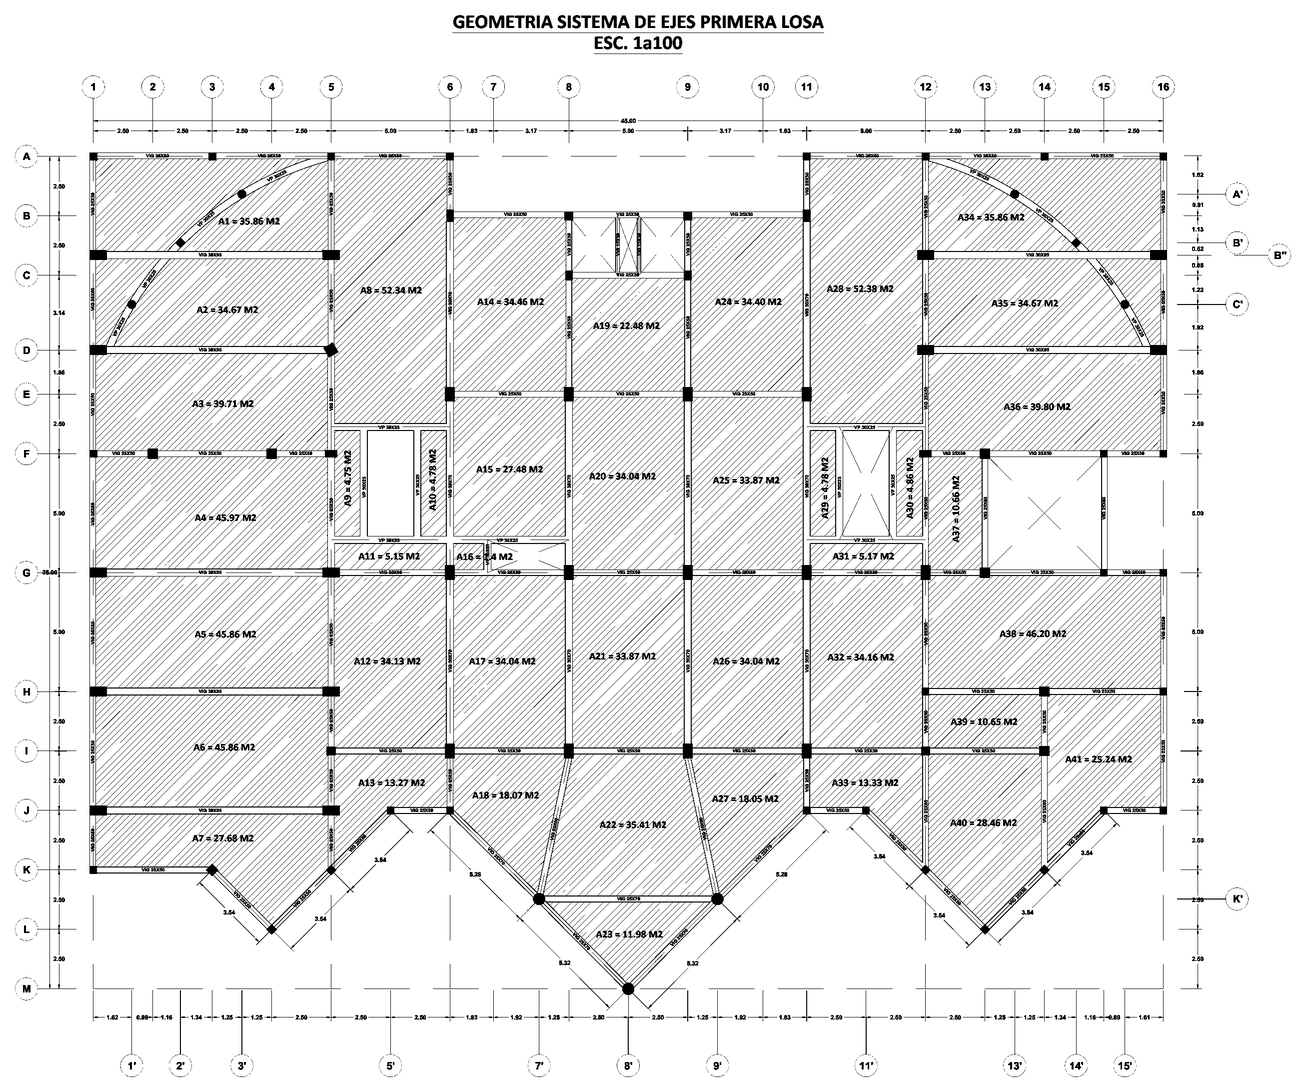
\includegraphics[width=\linewidth]{plano01_geometria_primera_losa}
\nota{Tomado del Plano~01 «Geometría sistema de ejes primera losa» (escala original 1:100). Las áreas A1 a A41 son los paños computados en el ítem~13.}
\end{figure}

La Tabla~\ref{tab:sistema} reúne las características del sistema según los documentos del proyecto. La ET define la losa como un sistema de viguetas pretensadas de fabricación industrial con complemento de plastoformo de 20~cm de altura, nervios, diafragmas y sus refuerzos, que se vacía de manera monolítica con las vigas y por franjas \parencite[p.~3]{uatf_et}. Los documentos no coinciden en la geometría del complemento, como se analiza en la Sección~\ref{sec:analisis-documental}.

\begin{table}[H]
\caption{Características de la losa alivianada según los documentos del proyecto}
\label{tab:sistema}
\setlength{\tabcolsep}{4pt}
\begin{tabularx}{\linewidth}{@{}P{4.0cm}LP{3.3cm}@{}}
\toprule
\textbf{Característica} & \textbf{Valor} & \textbf{Fuente} \\
\midrule
Espesor total & 25~cm: complemento de 20~cm y carpeta de 5~cm & ET, p.~3; PRETENSA \\
Altura del complemento en el corte & 0,15~m, con carpeta de 0,05~m & Plano~02 \\
Separación entre ejes de viguetas & 50~cm & PRETENSA \\
Luz máxima de vigueta & 7,50~m, simplemente apoyada & PRETENSA \\
Sobrecarga admisible & 400~kg/\mdos{} & PRETENSA \\
Viguetas & Hormigón de 350 a 400~kg/cm\textsuperscript{2}; acero de pretensado con rotura de 18.000~kg/cm\textsuperscript{2}; certificación IBNORCA e ISO & ET, p.~3 \\
Hormigón de carpeta y nervios & H25 (f'c~=~250~kg/cm\textsuperscript{2} a 28 días), cemento $\geq$~400~kg/\mtres{}; el fabricante exige al menos 21~MPa & ET, pp.~3--4; PRETENSA \\
Armadura de distribución & $\phi$6~c/20~cm en ambas direcciones & Plano~02 \\
Nervios transversales & Sección de 0,10~$\times$~0,15~m con 2~$\phi$10 inferiores y 2~$\phi$10 superiores & Plano~02 \\
Complemento según la ET & Plastoformo de 100~$\times$~50~$\times$~20~cm & ET, p.~3 \\
Complemento suministrado & Plastobloq de 20~$\times$~100~$\times$~44~cm, densidad 10~kg/\mtres{}, 2.350 piezas & UNICON \\
Medición y pago & Ítem~13 por \mdos{} (Bs~215,6753/\mdos{}); acero de la losa por kg en el ítem~8 (Bs~16,75584/kg) & PAO2, pp.~16, 20 \\
\bottomrule
\end{tabularx}
\nota{ET: especificaciones técnicas \parencite{uatf_et}; Plano~02: sección y detalles de la losa \parencite{uatf_planos}, reproducido en el Anexo de planos; PRETENSA: \textcite{pretensa2025}; UNICON: \textcite{unicon2025}; PAO2: \textcite{uatf2025pao2}.}
\end{table}

% =====================================================================
\section{Definición de factores y variables}
\label{sec:variables}

Los factores del modelo se dividen en controlables, que el SGC puede modificar (recepción de materiales, despacho por paño, inspección antes del vaciado, control del hormigón y conciliación de cantidades), y no controlables, que dependen del entorno (precios, clima y abastecimiento). La Tabla~\ref{tab:factores} relaciona cada factor o variable con su indicador y con la forma en que se trata en el modelo de la Sección~\ref{sec:modelo-simulacion}. Las dimensiones, indicadores e instrumentos de cada variable se detallan en el Anexo~\ref{anx:operacionalizacion}.

\begin{table}[H]
\caption{Factores, variables e indicadores del modelo}
\label{tab:factores}
\setlength{\tabcolsep}{4pt}
\begin{tabularx}{\linewidth}{@{}P{3.2cm}P{2.6cm}P{3.6cm}L@{}}
\toprule
\textbf{Factor o variable} & \textbf{Tipo} & \textbf{Indicador y unidad} & \textbf{Tratamiento en el modelo} \\
\midrule
SGC (control de materiales y del proceso) & Independiente ($X$); controlable & Cumplimiento ISO~9001 (\%); eficacias $e_i$ y $e_R$ & Escenario de tratamiento (con SGC) frente al de control (sin SGC) \\
Costo unitario de ejecución & Dependiente ($Y$) & $CU$ (Bs/\mdos{}), ecuación~\eqref{eq:cu} & Se descompone en costo directo teórico, CNC y costo de la calidad (ecuación~\ref{eq:cu-modelo}) \\
Desperdicio de materiales & Dependiente (HE1) & $IDM_i$ (\%), ecuación~\eqref{eq:idm} & Distribución triangular por material; línea base documentada o de literatura \\
Costo de no calidad & Dependiente (HE2) & $CNC$ (Bs/\mdos{}; \%), ecuación~\eqref{eq:cnc} & Desperdicio valorado más retrabajo (ecuación~\ref{eq:cnc-modelo}) \\
Costo de la calidad & Interviniente & $CC$ (Bs/\mdos{}) & Costos de prevención y evaluación del SGC repartidos en el saldo \\
Geometría de los paños & Controlada & Área, número y longitud de viguetas & Igual en ambos escenarios (paños homólogos) \\
Precios de los insumos & Controlada & Bs a precios del contrato & Constantes en ambos escenarios \\
Clima, abastecimiento e inflación & No controlable & Días de lluvia; demoras; variación de precios & Fuera del modelo de costos; se gestionan como riesgos del SGC \\
\bottomrule
\end{tabularx}
\nota{Elaboración propia. HE1 y HE2: hipótesis específicas. Las ecuaciones~\eqref{eq:cu-modelo} y \eqref{eq:cnc-modelo} se presentan en la Sección~\ref{sec:modelo-simulacion}.}
\end{table}

Los indicadores principales se calculan de la siguiente manera.

\textbf{Índice de desperdicio del material $i$:}
\begin{equation}
  IDM_i = \frac{Q_{\text{real},i} - Q_{\text{teórica},i}}{Q_{\text{teórica},i}} \times 100
  \label{eq:idm}
\end{equation}
donde $Q_{\text{real},i}$ es la cantidad consumida (entregada menos sobrante recuperable) y $Q_{\text{teórica},i}$ es la cantidad según planos y cómputos. En el modelo, $IDM_{i,s}$ es este mismo índice en el escenario $s$ (sin o con SGC), expresado como fracción. Como el hormigón solo puede medirse por vaciado, para ese material la unidad del indicador es el vaciado y su desperdicio se asigna a los paños en proporción a su volumen teórico.

\textbf{Costo unitario a precios constantes del contrato:}
\begin{equation}
  CU = \frac{\sum_{j} Q_{j}\, p_{j} + C_{MO} + C_{EQ}}{A}
  \label{eq:cu}
\end{equation}
donde $Q_j$ es la cantidad real del insumo $j$, $p_j$ su precio en el análisis de precios unitarios, $C_{MO}$ y $C_{EQ}$ los costos de mano de obra y equipo, y $A$ la superficie ejecutada (\mdos{}). Si en la ecuación~\eqref{eq:cu} se reemplaza la cantidad real por la teórica más el desperdicio, $Q_j = q_{teo,j}\,A\,(1 + IDM_j)$, el costo unitario se separa en el costo directo teórico ($CD_{teo}$), que no depende del SGC, y el costo del desperdicio, que sí depende de él. Esa separación es la base de la ecuación~\eqref{eq:cu-modelo}, que añade el retrabajo y el costo de la calidad.

\textbf{Costo de la calidad y costo de no calidad (modelo PAF):}
\begin{equation}
  CC = C_{P} + C_{E}, \qquad CNC = C_{FI} + C_{FE}, \qquad \%CNC = \frac{CNC}{C_{\text{ítem}}} \times 100
  \label{eq:cnc}
\end{equation}
donde $C_P$ son los costos de prevención, $C_E$ los de evaluación, $C_{FI}$ los de fallas internas (desperdicio, retrabajo y reparaciones) y $C_{FE}$ los de fallas externas (sobremediciones corregidas, ampliaciones y multas). El modelo de la Sección~\ref{sec:modelo-simulacion} cuantifica las fallas internas, que consumen recursos de la losa; las fallas externas de la línea base se documentan en el diagnóstico (Sección~\ref{sec:analisis-documental}), pero no se simulan, porque son correcciones de pago o sanciones y no consumo de materiales.

\textbf{Reducción relativa del costo en el paño homólogo $k$:}
\begin{equation}
  r_k = \frac{CU_{\text{sin},k} - CU_{\text{con},k}}{CU_{\text{sin},k}}
  \label{eq:reduccion}
\end{equation}
La ecuación~\eqref{eq:reduccion} es el indicador de la verificación futura con datos de obra, paño por paño (Sección~\ref{sec:verificacion-futura}); en la evaluación \emph{ex ante} se aplica al costo unitario del saldo completo (ecuación~\ref{eq:r-modelo}).

% =====================================================================
\section{Población y muestra}
\label{sec:poblacion}

\textbf{Población.} La población son las losas alivianadas con viguetas pretensadas de la fase contratada: tres losas con 3.344,44~\mdos{}, que es la cantidad del ítem~13 en el contrato modificado; la cantidad original era de 3.348,75~\mdos{} \parencite[p.~16]{uatf2025pao2}.

\textbf{Unidad de análisis.} La unidad de análisis es el paño de losa, delimitado por vigas y caracterizado por su área, el número y la longitud de sus viguetas y el número de complementos. Para el hormigón, la unidad es el vaciado (Sección~\ref{sec:variables}).

\textbf{Línea base censal.} La línea base estudia los 41 paños de la primera losa (1.109,84~\mdos{}), es decir, todos los paños ejecutados; por ello es un censo y no una muestra \parencite[p.~196]{hernandez2018}. Su elección no fue probabilística: es la única losa que se ejecutó antes de la resolución del contrato \parencite[p.~200]{hernandez2018}.

\textbf{Saldo y paños homólogos.} La evaluación \emph{ex ante} se aplica al saldo no ejecutado del ítem: 2.234,60~\mdos{} de la segunda y la tercera losa \parencite[p.~16]{uatf2025pao2}. El cómputo del contrato modificado calcula la «segunda y tercera losa» con los mismos 41 paños de la primera, cada uno multiplicado por dos \parencite[pp.~18--19]{uatf_item13}. Solo cambian cinco áreas: A1 y A34 (38,11~\mdos{} en lugar de 35,86), A2 y A35 (36,00 en lugar de 34,67) y A40 (28,76 en lugar de 28,46). Por ello cada losa superior mide 1.117,30~\mdos{}, 7,46~\mdos{} (0,7~\%) más que la primera, y las dos suman exactamente el saldo: $2 \times 1.117{,}30 = 2.234{,}60$~\mdos{} (cálculo propio). Como la geometría, el número de paños y el sistema de viguetas se repiten, los paños de las losas superiores se consideran homólogos de los de la primera, y el modelo aplica al saldo las cantidades teóricas por \mdos{} de la primera losa (Sección~\ref{sec:linea-base-cuantitativa}).

El mismo cómputo explica una pequeña diferencia documental. Su total es de 3.344,74~\mdos{}, porque registra la primera losa con 1.110,14~\mdos{} (A40 = 28,76~\mdos{}) \parencite[p.~18]{uatf_item13}; la tabla de tiempos de la contratista usa también 3.344,74~\mdos{} \parencite[p.~25]{uatf_item13}. El contrato modificado y las planillas, en cambio, consignan 3.344,44~\mdos{} \parencite[p.~16]{uatf2025pao2}: la diferencia de 0,30~\mdos{} corresponde al paño A40 de la primera losa, que se midió con 28,46~\mdos{} (cálculo propio).

% =====================================================================
\section{Diagnóstico de la situación actual (línea base)}
\label{sec:diagnostico}

El diagnóstico caracteriza la gestión de la calidad y el control de materiales con que se ejecutó la primera losa (OE1) y cuantifica su línea base (OE2). Tiene cuatro partes: las brechas frente a la norma ISO~9001:2026 (Sección~\ref{sec:brechas-iso}), el análisis documental de la primera losa (Sección~\ref{sec:analisis-documental}), las no conformidades y sus causas (Sección~\ref{sec:nc-causas}) y la línea base cuantitativa (Sección~\ref{sec:linea-base-cuantitativa}). Todos los hallazgos provienen de documentos del repositorio de la tesis y se citan con su página. Los que se refieren a cantidades o pagos se presentan como inconsistencias documentales que la Supervisión y la Fiscalización deben verificar con los respaldos que no forman parte de la documentación revisada; no constituyen una imputación de errores ni de pagos indebidos.

% ---------------------------------------------------------------------
\subsection{Brechas frente a la norma ISO~9001:2026}
\label{sec:brechas-iso}

Para medir la distancia entre la gestión real y los requisitos de la norma se aplicó, de manera documental, la lista de verificación C.1 del Anexo~\ref{anx:instrumentos}. La lista contiene 50 requisitos redactados por el autor para el proceso de la losa, a partir de la estructura de cláusulas 4 a 10 de la norma ISO~9001:2026 \parencite{iso9001_2026}; dos de ellos no aplican: el diseño y desarrollo, que corresponde al proyectista de la UATF, y la propiedad del cliente, porque la entidad no suministró materiales. Cada uno de los 48 requisitos aplicables se calificó con 1 (cumple), 0,5 (cumple parcialmente) o 0 (no cumple o sin evidencia documental), con la evidencia encontrada en los documentos y su página. El porcentaje de cada cláusula es la suma de las calificaciones dividida entre el número de requisitos aplicables. La Tabla~\ref{tab:brechas-iso} y la Figura~\ref{fig:brechas-iso} presentan los resultados y los comparan con dos diagnósticos bolivianos recientes.

\begin{table}[H]
\caption{Cumplimiento de los requisitos de ISO~9001 por cláusula: primera losa y diagnósticos de referencia}
\label{tab:brechas-iso}
\setlength{\tabcolsep}{4pt}
\begin{tabularx}{\linewidth}{@{}LQ{1.95cm}Q{1.45cm}Q{2.05cm}Q{2.15cm}Q{2.05cm}@{}}
\toprule
\textbf{Cláusula} & \textbf{Requisitos aplicables} & \textbf{Puntaje} & \textbf{Primera losa (esta tesis)} & \textbf{Mamani Calsina (2025)} & \textbf{Peña Callisaya (2024)} \\
\midrule
4. Contexto de la organización & 4 & 1,0 & 25,0~\% & 19~\% & 30~\% \\
5. Liderazgo & 5 & 1,0 & 20,0~\% & 38~\% & 60~\% \\
6. Planificación & 4 & 0,5 & 12,5~\% & 26~\% & 26~\% \\
7. Apoyo & 10 & 2,5 & 25,0~\% & 26~\% & 47~\% \\
8. Operación & 14 & 2,5 & 17,9~\% & 37~\% & 42~\% \\
9. Evaluación del desempeño & 6 & 1,5 & 25,0~\% & 11~\% & n.~e. \\
10. Mejora & 5 & 0,5 & 10,0~\% & 24~\% & n.~e. \\
\midrule
\textbf{Global} & \textbf{48} & \textbf{9,5} & \textbf{19,8~\%} & \textbf{24~\%} & \textbf{43~\%} \\
\bottomrule
\end{tabularx}
\nota{Elaboración propia con la lista de verificación C.1 (Anexo~\ref{anx:instrumentos}). Los diagnósticos de referencia corresponden a dos plantas industriales de viguetas pretensadas: Prensocret \parencite[pp.~47, 49]{mamanicalsina2025} e ISOCRET \parencite[p.~71]{pena2024}, evaluadas con la edición 2015 de la norma y con escalas de calificación propias. n.~e.: cláusula no evaluada. El cumplimiento global de esta tesis es el puntaje total entre los requisitos aplicables (9,5/48); el promedio simple de las siete cláusulas es 19,3~\%.}
\end{table}

\begin{figure}[H]
\centering
\caption{Cumplimiento de los requisitos de ISO~9001 por cláusula en la primera losa y en dos diagnósticos de referencia}
\label{fig:brechas-iso}
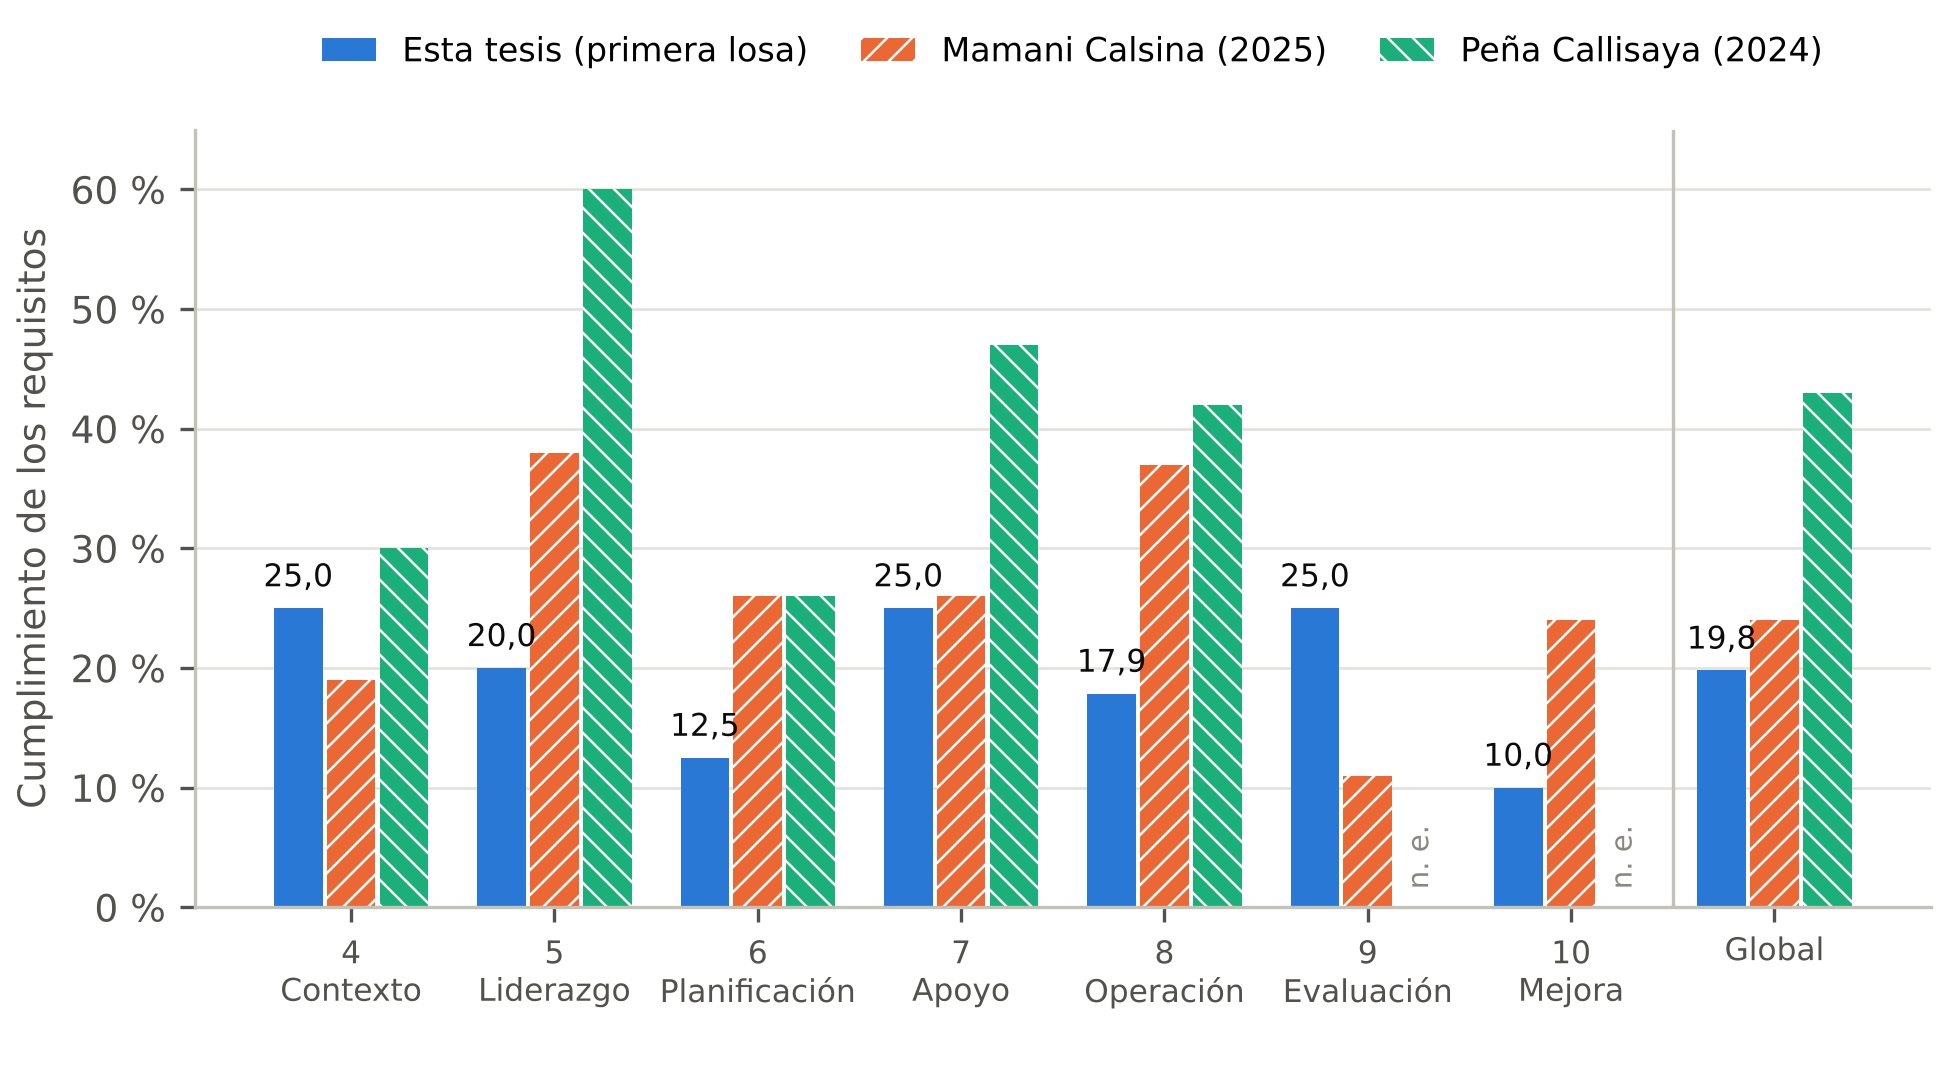
\includegraphics[width=\linewidth]{fig_brechas_iso9001}
\nota{Elaboración propia con los datos de la Tabla~\ref{tab:brechas-iso}. Las referencias son plantas de viguetas pretensadas \parencite{mamanicalsina2025,pena2024}; n.~e.: no evaluado. Figura generada con el script \texttt{cap2\_diagnostico\_figuras.py} de la carpeta de extracción de datos de obra.}
\end{figure}

El cumplimiento global fue de 19,8~\%. Ningún requisito alcanzó el cumplimiento pleno: 19 se cumplieron parcialmente y 29 no se cumplieron. Con la escala de \textcite[p.~42]{mamanicalsina2025}, todas las cláusulas se ubican en el rango «deficiente o no implementado» (0 a 25~\%); con el criterio de \textcite[p.~70]{pena2024}, que recomienda diseñar el sistema cuando el resultado no supera el 50~\%, el caso exige diseñar un SGC y no solo mejorar prácticas existentes. Las cláusulas más débiles fueron la mejora (10,0~\%), porque no hubo registro de no conformidades ni análisis de causas, y la planificación (12,5~\%), porque los riesgos de suministro, precios y clima no se identificaron antes de materializarse. La operación (17,9~\%) concentró la mayor cantidad de requisitos incumplidos (9 de 14), en particular el control del hormigón, la verificación de los suministros, la trazabilidad y el control de las salidas no conformes. Los puntajes parciales provienen sobre todo de controles contractuales que sí funcionaron: el Libro de Órdenes como canal de comunicación, la verificación del armado antes de cada vaciado, la medición conjunta de cantidades y los cambios contractuales tramitados formalmente.

El resultado es menor que el de las dos plantas industriales de viguetas pretensadas tomadas como referencia: 24~\% en Prensocret, con un mínimo de 11~\% en la evaluación del desempeño \parencite[pp.~48--49]{mamanicalsina2025}, y 43~\% en ISOCRET, con un mínimo de 26~\% en la planificación \parencite[p.~71]{pena2024}. La diferencia es coherente con la naturaleza de cada organización: una planta tiene procesos repetitivos, personal estable y documentación propia, mientras que la ejecución de una losa en una obra pública es un proceso temporal, cuyo control descansa casi por completo en la Supervisión. Coinciden, en cambio, en que la planificación, la evaluación y la mejora están entre las cláusulas más débiles. La comparación es solo indicativa, porque las escalas, la edición de la norma y las técnicas difieren: Peña Callisaya se basó en entrevistas y observación de los procesos \parencite[p.~67]{pena2024} y no evaluó las cláusulas 9 y 10.

\textbf{Limitación.} La evaluación fue documental y la realizó el investigador. Una calificación de 0 indica que el requisito no dejó evidencia en los documentos revisados, no que la práctica no haya existido. Las entrevistas de la guía C.7 (Anexo~\ref{anx:instrumentos}) a la Dirección de Obra, a la Supervisión y a la Fiscalización quedan como verificación complementaria. \pendiente{aplicar la guía de entrevista C.7 y ajustar, si corresponde, las calificaciones de la lista C.1.}

% ---------------------------------------------------------------------
\subsection{Análisis documental de la primera losa}
\label{sec:analisis-documental}

El análisis documental revisó, página por página, la Planilla de avance N.\textsuperscript{o}~2, de 139 páginas, que incluye el informe de Supervisión, los cómputos, los croquis, las fotografías, el certificado de laboratorio, los certificados de materiales, el contrato, el Libro de Órdenes y los cronogramas \parencite{uatf2025pao2}; la planilla y los cómputos de cierre \parencite{uatf_pao3}; el expediente del ítem~13 \parencite{uatf_item13}; las ET \parencite{uatf_et}, y los planos 01 a 03. Cada dato se contrastó en al menos dos fuentes. Las coincidencias confirmaron el dato; por ejemplo, las 41 áreas de paño y su total de 1.109,84~\mdos{} son idénticas en cuatro documentos. Las diferencias se registraron como hallazgos y se agrupan en siete temas.

\subsubsection{Control de la resistencia del hormigón}
El certificado de laboratorio N.\textsuperscript{o}~000293 es el único registro de ensayos de compresión adjunto a la Planilla N.\textsuperscript{o}~2. Comprende 12 probetas cilíndricas de 6~$\times$~12~pulgadas (área de 182,4~cm\textsuperscript{2}) de columnas y vigas, ensayadas el 5 de diciembre de 2025 a edades de 55 a 76 días y «proyectadas» a 28 días con un factor de tiempo (Tabla~\ref{tab:probetas}). El laboratorio aclaró que «las probetas fueron traidas [\textit{sic}] y elaboradas por la empresa solicitante» \parencite[p.~78]{uatf2025pao2}.

\begingroup\small\setstretch{1}\setlength{\tabcolsep}{4pt}
\begin{longtable}{@{}Q{0.8cm}P{1.7cm}Q{2.0cm}Q{1.2cm}Q{1.6cm}Q{2.4cm}Q{1.5cm}Q{2.4cm}@{}}
\caption{Resultados del certificado de laboratorio N.\textsuperscript{o}~000293 por probeta}\label{tab:probetas}\\
\toprule
\textbf{N.\textsuperscript{o}} & \textbf{Elemento} & \textbf{Fecha de la probeta} & \textbf{Edad (días)} & \textbf{Carga (kg)} & \textbf{Resistencia a la edad de ensayo (kg/cm\textsuperscript{2})} & \textbf{Factor de tiempo} & \textbf{Resistencia proyectada a 28 días (kg/cm\textsuperscript{2})} \\
\midrule
\endfirsthead
\multicolumn{8}{@{}l}{\textit{(continuación)}}\\
\toprule
\textbf{N.\textsuperscript{o}} & \textbf{Elemento} & \textbf{Fecha de la probeta} & \textbf{Edad (días)} & \textbf{Carga (kg)} & \textbf{Resistencia a la edad de ensayo (kg/cm\textsuperscript{2})} & \textbf{Factor de tiempo} & \textbf{Resistencia proyectada a 28 días (kg/cm\textsuperscript{2})} \\
\midrule
\endhead
\bottomrule
\endfoot
1 & Columna & 01/10/2025 & 65 & 56.200 & 308,1 & 0,877 & 270,2 \\
2 & Columna & 02/10/2025 & 64 & 53.200 & 291,6 & 0,879 & 256,2 \\
3 & Columna & 02/10/2025 & 64 & 53.600 & 293,8 & 0,879 & 258,2 \\
4 & Columna & 04/10/2025 & 62 & 56.000 & 307,0 & 0,882 & 270,8 \\
5 & Columna & 04/10/2025 & 62 & 55.000 & 301,5 & 0,882 & 266,0 \\
6 & Columna & 08/10/2025 & 58 & 59.000 & 323,4 & 0,890 & 287,8 \\
7 & Columna & 08/10/2025 & 58 & 52.000 & 285,1 & 0,890 & 253,6 \\
8 & Columna & 11/10/2025 & 55 & 54.000 & 296,0 & 0,896 & 265,3 \\
9 & Columna & 11/10/2025 & 55 & 55.000 & 301,5 & 0,896 & 270,2 \\
10 & Columna & 20/09/2025 & 76 & 58.000 & 318,0 & 0,861 & 273,7 \\
11 & Viga & 20/09/2025 & 76 & 55.400 & 303,7 & 0,861 & 261,4 \\
12 & Viga & 20/09/2025 & 76 & 53.400 & 292,7 & 0,861 & 252,0 \\
\midrule
\multicolumn{7}{@{}l}{Columnas ($n = 10$): media 267,2; desviación estándar 9,9; CV 3,7~\%} & 253,6 -- 287,8 \\
\multicolumn{7}{@{}l}{Vigas ($n = 2$): media 256,7; desviación estándar 6,6; CV 2,6~\%} & 252,0 -- 261,4 \\
\multicolumn{7}{@{}l}{Losa alivianada} & sin ensayos \\
\end{longtable}
\vspace{-6pt}
\nota{Transcrito del certificado del Laboratorio de Resistencia de Materiales y Tecnología del Hormigón de la Carrera de Ingeniería Civil de la UATF \parencite{labuatf2025}, adjunto a la Planilla de avance N.\textsuperscript{o}~2 \parencite[p.~78]{uatf2025pao2}. El certificado no tiene columna de fecha de ensayo; la fecha de la probeta más la edad coincide con el 05/12/2025 en las 12 filas. Estadísticos: cálculo propio. CV: coeficiente de variación.}
\endgroup

Los valores proyectados superan f'c~=~250~kg/cm\textsuperscript{2}, pero el control presenta cinco debilidades:
\begin{enumerate*}[label=(\roman*)]
  \item no hay probetas de la losa alivianada, aunque el criterio de superficie de ACI~318-25 exige al menos una muestra por cada $\approx$~464,5~\mdos{} de losa, es decir, al menos tres muestras para la primera losa \parencite[sección~26.12.2.1, p.~603]{aci318_2025};
  \item las probetas no se ensayaron a la edad especificada de 28 días, sino a 55--76 días, y se convirtieron con un factor de tiempo cuyo origen no se declara;
  \item las elaboró la propia contratista, sin muestreo independiente ni planilla de muestreo, cuando la norma exige que los ensayos del hormigón fresco y la elaboración de probetas estén a cargo de técnicos certificados \parencite[sección~26.12.1.1, p.~602]{aci318_2025};
  \item el certificado no identifica la muestra ni la amasada de cada probeta, de modo que no pueden formarse «ensayos de resistencia» como promedio de dos probetas de una misma muestra \parencite[sección~26.12.1.1, p.~601]{aci318_2025}; y
  \item cuatro de los doce valores están por debajo de 260~kg/cm\textsuperscript{2}, con poco margen sobre la resistencia especificada.
\end{enumerate*}
Además, la primera losa se certificó para pago el 8 de diciembre de 2025 \parencite[p.~16]{uatf2025pao2}, antes del 26 de diciembre, primera fecha en que su hormigón, vaciado después de la autorización del 28 de noviembre, podía cumplir 28 días (cálculo propio). En la documentación revisada no constan ensayos posteriores del hormigón de la losa.

\subsubsection{Recomendaciones y afirmaciones de la Supervisión}
En su informe de la Planilla N.\textsuperscript{o}~2, la Supervisión recomendó a la contratista «presentar las garantías de todos los materiales empleados en obra», «realizar la rotura de probetas de los elementos vaciados» y «presentar las dosificaciones para los diferentes tipos de elementos» \parencite[p.~9]{uatf2025pao2}. Al cierre del periodo en que se ejecutó la losa no se contaba, por tanto, con esos controles básicos. Dos páginas después, el mismo informe afirma que «los trabajos realizados durante el periodo presentan buena calidad», que se verificaron los materiales, los encofrados y las armaduras, y que se realizó la rotura de probetas en el laboratorio de la UATF \parencite[p.~11]{uatf2025pao2}. Ninguna de las dos páginas indica qué elementos se ensayaron ni con qué registros se verificaron los materiales. La calificación de la calidad carece de evidencia objetiva y contradice las recomendaciones de la p.~9; para la losa, el único certificado disponible no contiene ninguna probeta.

\subsubsection{Libro de Órdenes}
La copia del Libro de Órdenes adjunta a la Planilla N.\textsuperscript{o}~2 comprende 12 hojas notariales (N.\textsuperscript{o}~000019 a 000030) con 24 asientos, del 10 de septiembre al 28 de noviembre de 2025 \parencite[pp.~114--125]{uatf2025pao2}. La Tabla~\ref{tab:libro-ordenes} resume su contenido.

\begin{table}[H]
\caption{Síntesis del Libro de Órdenes del periodo de ejecución de la primera losa}
\label{tab:libro-ordenes}
\setlength{\tabcolsep}{4pt}
\begin{tabularx}{\linewidth}{@{}P{5.4cm}P{2.8cm}L@{}}
\toprule
\textbf{Indicador} & \textbf{Valor} & \textbf{Observación} \\
\midrule
Asientos & 24 (12 del Director de Obra y 12 de la Supervisión) & Respuesta de la Supervisión el mismo día en los 12 casos \\
Solicitudes de verificación y vaciado & 8 & 8 autorizadas el mismo día (100~\%) \\
Elementos cuyo vaciado se autorizó & 5 columnas de arranque, 7 ejes de vigas de arriostre, 75 columnas y la losa del primer nivel & La losa, el 28/11/2025, «desde dos frentes» \\
No conformidades, rechazos, órdenes de corrección o retrabajos & 0 & Ningún asiento registra defectos \\
Instrucciones de calidad & 3 específicas y 3 genéricas & Dosificación (23/10); contenido de agua y toma de muestras (31/10); especificaciones, dosificaciones y curado (28/11), sin registro asociado \\
Instrucción de muestreo al autorizar la losa & No & Sí se instruyó el 31/10/2025 para columnas \\
Días de lluvia notificados & 7 & 09/09, 14/09, 17/09, 15/10, 12/11, 13/11 y 21/11/2025 \\
Demoras de materiales por escasez de combustible & 1 asiento & 17/11/2025 \\
Constancia firmada del Director de Obra & 0 de 12 hojas & Exigida por la cláusula 25.ª \\
Encabezado (contratante, obra, fecha) & Vacío en las 12 hojas & --- \\
\bottomrule
\end{tabularx}
\nota{Elaborado con base en \textcite[pp.~100, 114--125]{uatf2025pao2}. Cálculos propios sobre la transcripción completa de los 24 asientos.}
\end{table}

El Libro de Órdenes funcionó como canal de comunicación, pero no como registro de control de la calidad. Todas las solicitudes se aprobaron el mismo día sin observaciones; las instrucciones sobre dosificación, contenido de agua y curado se repitieron sin que conste una dosificación aprobada, un control de asentamiento o un registro de curado. El 28 de noviembre de 2025 la Supervisión informó que había verificado «la losa, instalaciones, agregados, etc.» y autorizó el vaciado «desde dos frentes»; a diferencia de la autorización del 31 de octubre para columnas, no instruyó tomar probetas \parencite[pp.~121, 125]{uatf2025pao2}. No se registró la fecha real del hormigonado; como la losa se certificó completa en la planilla cerrada el 8 de diciembre, se infiere que se vació entre esas dos fechas. Que no haya no conformidades registradas no prueba que no hubiera defectos: muestra que el instrumento contractual de control no dejó constancia de ellos. Los asientos posteriores, copiados en el expediente del ítem~13, registran la autorización del vaciado de las columnas del segundo nivel, el 16 de diciembre, y la carta notariada del 5 de enero de 2026 \parencite[pp.~13--14]{uatf_item13}.

\subsubsection{Coherencia técnica de los documentos}
Los documentos del proyecto describen de manera distinta el complemento de la losa:
\begin{enumerate*}[label=(\alph*)]
  \item la ET exige plastoformo de 100~$\times$~50~$\times$~20~cm \parencite[p.~3]{uatf_et};
  \item el corte transversal del Plano~02 acota un complemento de 0,15~m de altura con una carpeta de 0,05~m, es decir, una losa de 20~cm \parencite[Plano~02]{uatf_planos}; y
  \item el certificado del proveedor corresponde a 2.350 piezas de Plastobloq de 20~$\times$~100~$\times$~44~cm \parencite{unicon2025}, compatibles con la separación de 50~cm entre ejes de viguetas que indica el fabricante de las viguetas \parencite{pretensa2025}.
\end{enumerate*}
Además, mientras que la ET y el ítem~13 describen una losa de «h~=~25~cm» y el certificado del fabricante de las viguetas indica 20~+~5~=~25~cm \parencite{pretensa2025}, la sección de 0,20~m del Plano~02 no alcanzaría la altura mínima de 250~mm, incluida la carpeta de compresión, que la NBDS exige para que una losa de viguetas prefabricadas funcione como diafragma rígido \parencite[art.~12.I, inc.~b, p.~22]{mopsv2023nbds}, lo que refuerza que se trata de un error del plano que la Supervisión debe aclarar. No se encontró una orden de cambio ni una aclaración que resuelva estas diferencias. Los planos tampoco son completos ni del todo coherentes. El Plano~02 detalla un nervio transversal de 0,10~$\times$~0,15~m con cuatro barras de $\phi$10 y la armadura de momentos negativos sobre los apoyos, pero ningún plano ubica los nervios ni fija el diámetro, la separación o la longitud de los negativos: las leyendas remiten a una «armadura de acuerdo a planos» que no figura en el juego de planos revisado. En el Plano~03, la etiqueta del paño A7 indica 10 viguetas y hay 19 dibujadas; los paños A34 a A36 y A38 llevan la etiqueta 20 y tienen 18 o 19 viguetas dibujadas; y el paño A16 tiene la etiqueta 2 sin viguetas dibujadas \parencite{uatf_planos}. Estas omisiones impiden calcular sin supuestos la cantidad teórica de acero, que es justamente la base para controlar lo que se mide y se paga (Sección~\ref{sec:linea-base-cuantitativa}). Además, la ET exige cumplir la norma CBH-87 y las normas bolivianas de cemento (NB~2.1-001 a 2.1-014), áridos (NB~596-91 a 612-91) y agua (NB~587-91 y 588-91) \parencite[pp.~1--2]{uatf_et}, y no menciona la NB~1225001, basada en el código ACI~318. Por último, la ET del ítem~13 incluye entre los materiales del ítem el «fierro corrugado (parrilla de compresión y refuerzo momentos negativos)» \parencite[p.~3]{uatf_et}, mientras que el acero de la losa se midió y pagó en el ítem~8 \parencite[p.~20]{uatf2025pao2}. Sin el análisis de precios unitarios contractual del ítem~13, que no forma parte de la documentación revisada, no puede saberse si ese precio incluye el acero; la superposición debe verificarse.

\subsubsection{Control de cantidades}
\textbf{Ítem~13.} La primera losa se certificó completa en la Planilla N.\textsuperscript{o}~2: 1.109,84~\mdos{} por Bs~239.365,07, el 33,18~\% de la cantidad modificada, sin avance anterior \parencite[p.~16]{uatf2025pao2}. El cómputo lista los 41 paños solo con su área, sin dimensiones ni cantidades de materiales \parencite[pp.~28--29]{uatf2025pao2}.

\textbf{Acero de la losa.} En el mismo periodo, el ítem~8 certificó 13.548,49~kg (Bs~227.016,33): 9.377,31~kg de vigas y una línea «LOSA ALIVIANADA» de 1,00~$\times$~4.171,18~kg, anotada en las columnas de largo y volumen y sin planilla de armado que la respalde \parencite[pp.~19--20]{uatf2025pao2}. Esa cantidad equivale a 3,76~kg/\mdos{} (cálculo propio) y se compara con la cantidad teórica en la Sección~\ref{sec:linea-base-cuantitativa}.

\textbf{Planilla de cierre en dos versiones.} El documento oficial de cierre es la Planilla de avance N.\textsuperscript{o}~3 firmada el 16 de marzo de 2026, que paga Bs~16.837,41 en el periodo, llega a un avance total de Bs~2.073.392,68 (57,43~\%) y descuenta 1.862,81~kg de acero (Bs~$-$31.212,95), el 3,55~\% de los 52.424,65~kg acumulados; el acumulado del ítem~8 queda en 50.561,84~kg, la misma cifra que usa el detalle de descuento por agua potable \parencite[pp.~2, 12]{uatf_item13}. Existe una segunda versión del mismo documento en archivo digital, que descuenta 1.915,16~kg (Bs~$-$32.090,11; 3,65~\%), deja un acumulado de 50.509,49~kg, paga además la limpieza general (Bs~2.566,96) y suma Bs~18.527,21 en el periodo y 57,48~\% de avance \parencite{uatf_pao3}. Las dos versiones difieren en 52,35~kg de acero ($\approx$~Bs~877,17) y en el pago de la limpieza general; la Supervisión y la Fiscalización deben verificar cuál se tramitó. El cómputo métrico de la versión digital es, además, la única fuente que desglosa el acero por elementos: en él, la línea de la losa aparece como 3~$\times$~4.171,18~kg~=~12.513,54~kg, aunque solo se ejecutó una losa \parencite[hoja «Cómputos métricos», filas 375--541]{uatf_pao3}. Como el total de ese cómputo bajó respecto del acumulado anterior, las demás partidas debieron bajar 10.257,78~kg. La Tabla~\ref{tab:acero-grupos} concilia ambos documentos por grupos de elementos.

\begin{table}[H]
\caption{Conciliación del acero acumulado entre la Planilla N.\textsuperscript{o}~2 y el cómputo de cierre, por grupos de elementos}
\label{tab:acero-grupos}
\setlength{\tabcolsep}{4pt}
\begin{tabularx}{\linewidth}{@{}P{5.0cm}RRR@{}}
\toprule
\textbf{Grupo de elementos} & \textbf{Acumulado en la PAO~N.\textsuperscript{o}~2 (kg)} & \textbf{Cómputo de cierre, versión digital (kg)} & \textbf{Diferencia (kg)} \\
\midrule
Zapatas a encalzar y zapatas nuevas & \multirow{3}{*}{38.876,16\textsuperscript{a}} & 8.527,47 & \multirow{3}{*}{$-$10.215,02} \\
Columnas a encamisar, nuevas y que se mantienen & & 17.780,20 & \\
Vigas de arriostre & & 2.353,47 & \\
Vigas de H\textsuperscript{o}A\textsuperscript{o} & 9.377,31 & 9.334,55 & $-$42,76 \\
Losa alivianada & 4.171,18 (1~$\times$~4.171,18) & 12.513,54 (3~$\times$~4.171,18) & +8.342,36 \\
Gradas del primer nivel & --- & 773,92\textsuperscript{b} & --- \\
\midrule
Total del cómputo de cierre (versión digital) & 52.424,65 & 50.509,23 & $-$1.915,42 \\
Planilla de cierre, versión digital & 52.424,65 & 50.509,49 & $-$1.915,16 \\
Planilla de cierre firmada (oficial) y descuento por agua potable & 52.424,65 & 50.561,84\textsuperscript{c} & $-$1.862,81 \\
\bottomrule
\end{tabularx}
\nota{Elaboración propia (cálculos propios) con base en \textcite[pp.~16, 19--20]{uatf2025pao2}, \textcite{uatf_pao3} (hoja «Cómputos métricos», filas 375 a 541; subtotales por grupo: zapatas a encalzar 3.629,47; zapatas nuevas 4.898,00; columnas a encamisar 4.170,02; columnas nuevas 11.395,18; columnas que se mantienen 2.215,00) y \textcite[pp.~2, 12]{uatf_item13}. \textsuperscript{a}~Avance de la Planilla N.\textsuperscript{o}~1, sin desglose por elementos en los documentos revisados; por diferencia corresponde a los elementos distintos de las vigas y la losa. \textsuperscript{b}~Anotado sin cantidad parcial; no se suma al total. \textsuperscript{c}~Sin desglose por elementos: la versión firmada no adjunta un cómputo del acero.}
\end{table}

La conciliación muestra cuatro inconsistencias que la Supervisión y la Fiscalización deben verificar. Primera, la línea de la losa pasa de 1 a 3 veces 4.171,18~kg sin respaldo, lo que llevaría la cuantía a 11,28~kg/\mdos{} para la losa ejecutada. Segunda, la reducción de 10.215,02~kg en zapatas, columnas y vigas de arriostre no tiene explicación línea por línea; con la documentación disponible no puede saberse cuál de las dos cifras es la correcta. Tercera, coexisten tres cifras del acero acumulado: 52.424,65~kg en la Planilla N.\textsuperscript{o}~2, 50.561,84~kg en la planilla de cierre firmada y 50.509,49~kg en su versión digital, más un total de 50.509,23~kg en el cómputo de la versión digital, que difiere en 0,26~kg de su propia planilla. Cuarta, la tabla de tiempos con la que la contratista sustentó la ampliación de plazo N.\textsuperscript{o}~2 usa para el ítem~8 una cantidad autorizada de 85.777,46~kg, 7.797,95~kg más que los 77.979,51~kg del contrato modificatorio \parencite[pp.~17, 25]{uatf_item13}. A esto se suma la posible superposición del acero de la losa entre los ítems~8 y~13 descrita antes. En conjunto, estos hallazgos no prueban un error ni un pago indebido, pero muestran que las cantidades se controlaron al cierre del contrato y no en el mes en que se originaron, que es lo que el procedimiento de conciliación del SGC propone corregir (Sección~\ref{sec:sgc-operacion}).

\textbf{Otras correcciones.} La Planilla N.\textsuperscript{o}~2 corrigió la excavación del ítem~4 en $-$5,66~\mtres{} (Bs~$-$403,14), porque la Planilla N.\textsuperscript{o}~1 había certificado más de lo que luego se computó \parencite[pp.~16, 18]{uatf2025pao2}. Además, las cantidades del contrato original y del actualizado difieren entre $-$80,8~\% y +46,7~\% según el ítem (acero, +32,1~\%; hormigón de zapatas, +16,0~\%; escaleras, +46,7~\%; columnas, $-$8,5~\%; vigas, $-$7,9~\%), y la Supervisión anunció otra orden de cambio por incremento de volúmenes \parencite[pp.~11, 16]{uatf2025pao2}.

\subsubsection{Suministro y gestión de materiales}
El abastecimiento fue el punto más expuesto al entorno. La Supervisión informó que se hicieron «modificaciones estructurales debido a la inexistencia de viguetas en el mercado de los tamaños requeridos» \parencite[p.~11]{uatf2025pao2}, sin que se adjunte un documento que describa el cambio, su cálculo o su aprobación. El distribuidor de acero comunicó el 16 de junio de 2025 que, de una compra de 20 toneladas de fierro corrugado, solo había entregado el 30~\%, por el desabastecimiento de combustibles y los bloqueos de carreteras \parencite{laslomas2025}, y el 17 de noviembre de 2025, en pleno armado de la losa, la contratista informó que los materiales tardaban mucho en llegar por la misma causa \parencite[p.~123]{uatf2025pao2}. Ninguno de estos hechos dio lugar a una acción documentada sobre los proveedores ni a un plan de compras anticipado.

La recepción de materiales fue documental y tardía. Los certificados de PRETENSA y de UNICON están fechados el 27 de noviembre de 2025, después de que comenzara el armado de la losa (14 de noviembre); no llevan firma, y el de las viguetas no indica cantidad, lote ni resultados de ensayo \parencite[pp.~80--81, 122]{uatf2025pao2}. Los certificados de acero corresponden a barras de 20, 16, 12, 9,5 y 8~mm producidas entre abril y mayo de 2025 y emitidos al distribuidor; no hay certificados de las barras de 6 y 10~mm que, según el Plano~02, forman la parrilla y los nervios de la losa, ni de cemento y áridos \parencite[pp.~82--86]{uatf2025pao2}. La masa lineal certificada de las barras es entre 1,8~\% y 5,8~\% menor que la nominal (cálculo propio): un balance por peso que no lo considere confundiría esa diferencia con desperdicio.

La gestión de los materiales en obra fue mínima. El plan de acopio de la contratista «consiste en transportar el material y ubicarlo cerca de la obra con el resguardo necesario y satisfactorio» \parencite[p.~10]{uatf2025pao2}, sin criterios de recepción, almacenamiento ni control de existencias, pese a que el contrato exige acopiar en zonas aprobadas e inspeccionar los materiales antes de su uso \parencite[p.~102]{uatf2025pao2}. No se encontraron notas de remisión, kardex ni vales de salida. De las 2.350 piezas de EPS entregadas \parencite{unicon2025} no consta cuántas se colocaron, cuántas sobraron ni si toda la entrega correspondió a la primera losa. Las fotografías muestran material y restos dispersos en el terreno, el vaciado con carretillas y la parrilla de la carpeta pisada durante el hormigonado, sin separadores visibles a la resolución disponible \parencite[pp.~75--76]{uatf2025pao2}; ese tránsito sobre los complementos colocados es una causa conocida de mayor consumo de hormigón de la carpeta \parencite{concretec2016plastoformo}.

\subsubsection{Planificación y plazo}
El cronograma de actividades «actualizado» a 360 días programó la losa alivianada del 23 de diciembre de 2025 al 21 de abril de 2026 y todo el acero estructural del 19 de junio al 28 de julio de 2025 \parencite[p.~137]{uatf2025pao2}. Según el Libro de Órdenes, la losa se armó en noviembre y su vaciado se autorizó el 28 de noviembre, 25 días antes del inicio programado, y el acero se armó entre septiembre y noviembre \parencite[pp.~114--125]{uatf2025pao2}. El cronograma, que el contrato define como documento fundamental de control \parencite[p.~105]{uatf2025pao2}, no reflejaba la secuencia real. Al 8 de diciembre de 2025 el avance acumulado era de 56,97~\% frente a 60,00~\% previsto: un retraso de 3,03 puntos que la Supervisión reconoció \parencite[p.~10]{uatf2025pao2}. El mismo informe consigna un «desfase del periodo» de 3,03~\%, cuando el del periodo es de 1,07~\% (29,00~\% previsto frente a 27,93~\% ejecutado; cálculo propio). Con el cronograma de desembolsos, interpolado linealmente entre los días 209 y 270, el avance previsto al 8 de diciembre sería de $\approx$~63,8~\% (cálculo propio con supuestos) \parencite[p.~139]{uatf2025pao2}.

\subsubsection{Otros hallazgos de control documental}
Se registraron además inconsistencias menores que muestran un control débil de la información documentada: el certificado de avance consigna un anticipo del 10~\% en un contrato sin anticipo \parencite[p.~14]{uatf2025pao2}; una columna tipo~5 tiene 6 unidades en el rótulo y 7 en la planilla de armado, y una hoja de armado está duplicada \parencite[pp.~38, 51--52]{uatf2025pao2}; las boletas de garantía vencen el 14 de abril de 2026, 16 días antes de la entrega provisional vigente, y equivalen al 7~\% del monto original \parencite[pp.~130--131]{uatf2025pao2}; dos de los tres certificados del seguro obligatorio de accidentes adjuntos vencieron el 3 de junio de 2025 \parencite[pp.~134--135]{uatf2025pao2}; el contrato seguía sin protocolizar al 8 de diciembre de 2025 \parencite[p.~88]{uatf2025pao2}; y el archivo de la planilla de cierre conserva una hoja de un contrato de 2023 de otra empresa \parencite{uatf_pao3}.

% ---------------------------------------------------------------------
\subsection{No conformidades y análisis de causas}
\label{sec:nc-causas}

A partir del análisis documental y de la lista de verificación, el investigador identificó 22 no conformidades (NC) respecto de los requisitos de la norma ISO~9001:2026, del contrato, de las ET y de la normativa del hormigón (Tabla~\ref{tab:nc}). Cada NC se clasificó en una categoría del método 6M (materiales, método, mano de obra, medición, maquinaria y medio ambiente) o en la categoría de gestión, que reúne las fallas de planificación, documentación y dirección. Como no existe un registro de NC de la obra, la tabla es una reconstrucción documental y no un registro levantado durante la ejecución.

\begingroup\small\setstretch{1}\setlength{\tabcolsep}{3pt}
\begin{longtable}{@{}P{1.3cm}P{5.7cm}P{2.6cm}P{3.6cm}P{2.0cm}@{}}
\caption{No conformidades identificadas en la ejecución de la primera losa}\label{tab:nc}\\
\toprule
\textbf{Código} & \textbf{Descripción} & \textbf{Evidencia} & \textbf{Requisito afectado} & \textbf{Categoría} \\
\midrule
\endfirsthead
\multicolumn{5}{@{}l}{\textit{(continuación)}}\\
\toprule
\textbf{Código} & \textbf{Descripción} & \textbf{Evidencia} & \textbf{Requisito afectado} & \textbf{Categoría} \\
\midrule
\endhead
\bottomrule
\endfoot
NC-01 & El hormigón de la losa no tiene ensayos de resistencia; la losa se certificó para pago antes de la primera fecha en que podía tener 28 días & PAO2, pp.~16, 78, 125 & ISO 8.5.1 y 8.6; ACI~318-25, 26.12; cl.~26.6 & Medición \\
NC-02 & Probetas de columnas y vigas ensayadas a 55--76 días y proyectadas con un factor sin fuente; elaboradas por la contratista y sin identificación de la muestra & PAO2, p.~78 & ISO 7.1.5 y 8.5.2; ACI~318-25, 26.12 & Medición \\
NC-03 & Sin dosificación aprobada ni registros de asentamiento y curado, pese a tres instrucciones de la Supervisión & PAO2, pp.~9, 120, 121, 125 & ISO 8.5.1; ET; ACI~318-25, 26.4 y 26.5 & Método \\
NC-04 & Certificados de viguetas y EPS posteriores al inicio del armado y sin firma; el de viguetas sin cantidad, lote ni ensayos; sin inspección de recepción & PAO2, pp.~80--81, 122 & ISO 8.4.2; cl.~26.6 & Materiales \\
NC-05 & Sin certificados de las barras de $\phi$6 y $\phi$10 de la losa, ni de cemento y áridos & PAO2, pp.~82--86; Plano~02 & ISO 8.4.2; ET; ACI~318-25, 26.6 & Materiales \\
NC-06 & Tres geometrías del complemento EPS (ET, Plano~02 y certificado) sin aclaración ni orden de cambio & ET, p.~3; Plano~02; PAO2, p.~81 & ISO 7.5.3 y 8.2.3 & Gestión \\
NC-07 & ET con la CBH-87 y normas bolivianas antiguas de cemento, áridos y agua & ET, pp.~1--2 & ISO 7.5.3 y 8.2.2 & Gestión \\
NC-08 & Modificaciones estructurales por falta de viguetas de los tamaños requeridos, sin documento del cambio ni de su aprobación & PAO2, p.~11 & ISO 6.3, 8.4.1 y 8.5.6 & Materiales \\
NC-09 & Libro de Órdenes con encabezados vacíos y sin la constancia firmada del Director de Obra en las 12 hojas & PAO2, pp.~114--125 & ISO 7.4 y 7.5.2; cl.~25.ª & Gestión \\
NC-10 & Liberaciones de vaciado sin lista de verificación ni criterios; la de la losa no instruye muestreo ni registra la fecha del hormigonado & PAO2, pp.~114--125 & ISO 8.5.1 y 8.6; ACI~318-25, 26.13 & Método \\
NC-11 & Ninguna no conformidad, rechazo o retrabajo registrado en el periodo & PAO2, pp.~6--11, 114--125 & ISO 8.7 y 10.2 & Gestión \\
NC-12 & Calidad calificada de «buena» y ensayos y verificaciones afirmados sin registros, en contradicción con las recomendaciones de la misma Supervisión & PAO2, pp.~9, 11 & ISO 9.1.2 y 9.1.3 & Medición \\
NC-13 & Acero de la losa computado en el ítem~8 sin planilla de armado; la ET del ítem~13 incluye la parrilla y los negativos (posible doble cómputo, a verificar) & PAO2, p.~20; ET, p.~3 & ISO 9.1.1; cl.~27.ª & Medición \\
NC-14 & Cómputo de cierre con 3~$\times$~4.171,18~kg para una sola losa; dos versiones de la planilla de cierre y tres cifras del acero acumulado (a conciliar) & PAO3; PAO2, p.~16; Exp., pp.~2, 12 & ISO 7.5.3 y 9.1.1; cl.~27.ª & Medición \\
NC-15 & Cantidades corregidas después de pagadas (ítem~4 y acero) sin análisis de causas & PAO2, pp.~16, 18; PAO3 & ISO 10.2 & Medición \\
NC-16 & Sin cantidades de materiales por paño ni control de consumos; 2.350 piezas de EPS entregadas sin conciliación con lo colocado & PAO2, pp.~28--29, 81 & ISO 8.1 y 8.5.2 & Materiales \\
NC-17 & Acopio sin recepción, inspección, inventario ni protección; material y restos dispersos & PAO2, pp.~10, 75--76 & ISO 8.5.4; cl.~26.9 & Método \\
NC-18 & Parrilla sin separadores visibles y pisada durante el vaciado (observación fotográfica por confirmar) & PAO2, p.~76 & ISO 7.3 y 8.5.1; ACI~318-25, 26.6 & Mano de obra \\
NC-19 & Competencia y capacitación del personal de obra no determinadas ni registradas; Supervisión con apoyo de pasantes & PAO2, pp.~9--10 & ISO 7.2 & Mano de obra \\
NC-20 & Cronograma «actualizado» que no refleja la ejecución; retraso de 3,03 puntos y desfase del periodo mal calculado & PAO2, pp.~10, 137 & ISO 6.2, 8.1 y 9.1.3; cl.~32.ª & Gestión \\
NC-21 & Riesgos de suministro y de precios no identificados ni tratados (combustible, acero, viguetas) & PAO2, pp.~11, 123; Las Lomas & ISO 6.1 & Gestión \\
NC-22 & Sin previsiones para lluvias y bajas temperaturas en el vaciado y el curado & PAO2, pp.~122, 124 & ISO 6.1 y 7.1.4; ACI~318-25, 26.5 & Medio ambiente \\
\end{longtable}
\vspace{-6pt}
\nota{Elaboración propia. PAO2: \textcite{uatf2025pao2}; PAO3: \textcite{uatf_pao3}; Exp.: \textcite{uatf_item13}; ET: \textcite{uatf_et}; Las Lomas: \textcite{laslomas2025}; ACI~318-25: \textcite{aci318_2025}; cl.: cláusula del contrato. Los numerales de ISO~9001 corresponden a la lista C.1.}
\endgroup

Las NC se relacionan con las nueve brechas que orientan el diseño del SGC (Sección~\ref{sec:diseno-sgc}): el control del hormigón (B1) agrupa las NC-01 a NC-03 y la NC-10; las evidencias de conformidad entregadas solo a pedido (B2), las NC-04, NC-05 y NC-12; la información documentada incoherente (B3), las NC-06, NC-07 y NC-09; el control de cantidades (B4), las NC-13 a NC-15; la falta de registro de consumos (B5), las NC-16 y NC-17; la falta de puntos de inspección (B6), las NC-10, NC-18 y NC-19; la falta de registro de NC y de costos de la calidad (B7), la NC-11; los riesgos de suministro y precios (B8), las NC-08, NC-20 y NC-21; y el clima (B9), la NC-22.

\textbf{Diagrama de Pareto.} La Figura~\ref{fig:pareto-nc} ordena las NC por categoría. La medición y la gestión reúnen 12 de las 22 NC (54,5~\%); con los materiales llegan al 72,7~\% y con el método, al 86,4~\%. Esta concentración es coherente con la regla de Pareto, según la cual pocos factores explican la mayor parte de los problemas de calidad de una obra \parencite[p.~70]{alfaro2011}. Las «pocas causas vitales» de la primera losa no están en la mano de obra ni en el clima, sino en la ausencia de un sistema que mida, registre y concilie: ensayos, recepción de materiales, consumos y cantidades. No se identificaron NC en la categoría de maquinaria; el vaciado con carretillas se consideró parte del método.

\begin{figure}[H]
\centering
\caption{Diagrama de Pareto de las no conformidades de la primera losa por categoría}
\label{fig:pareto-nc}
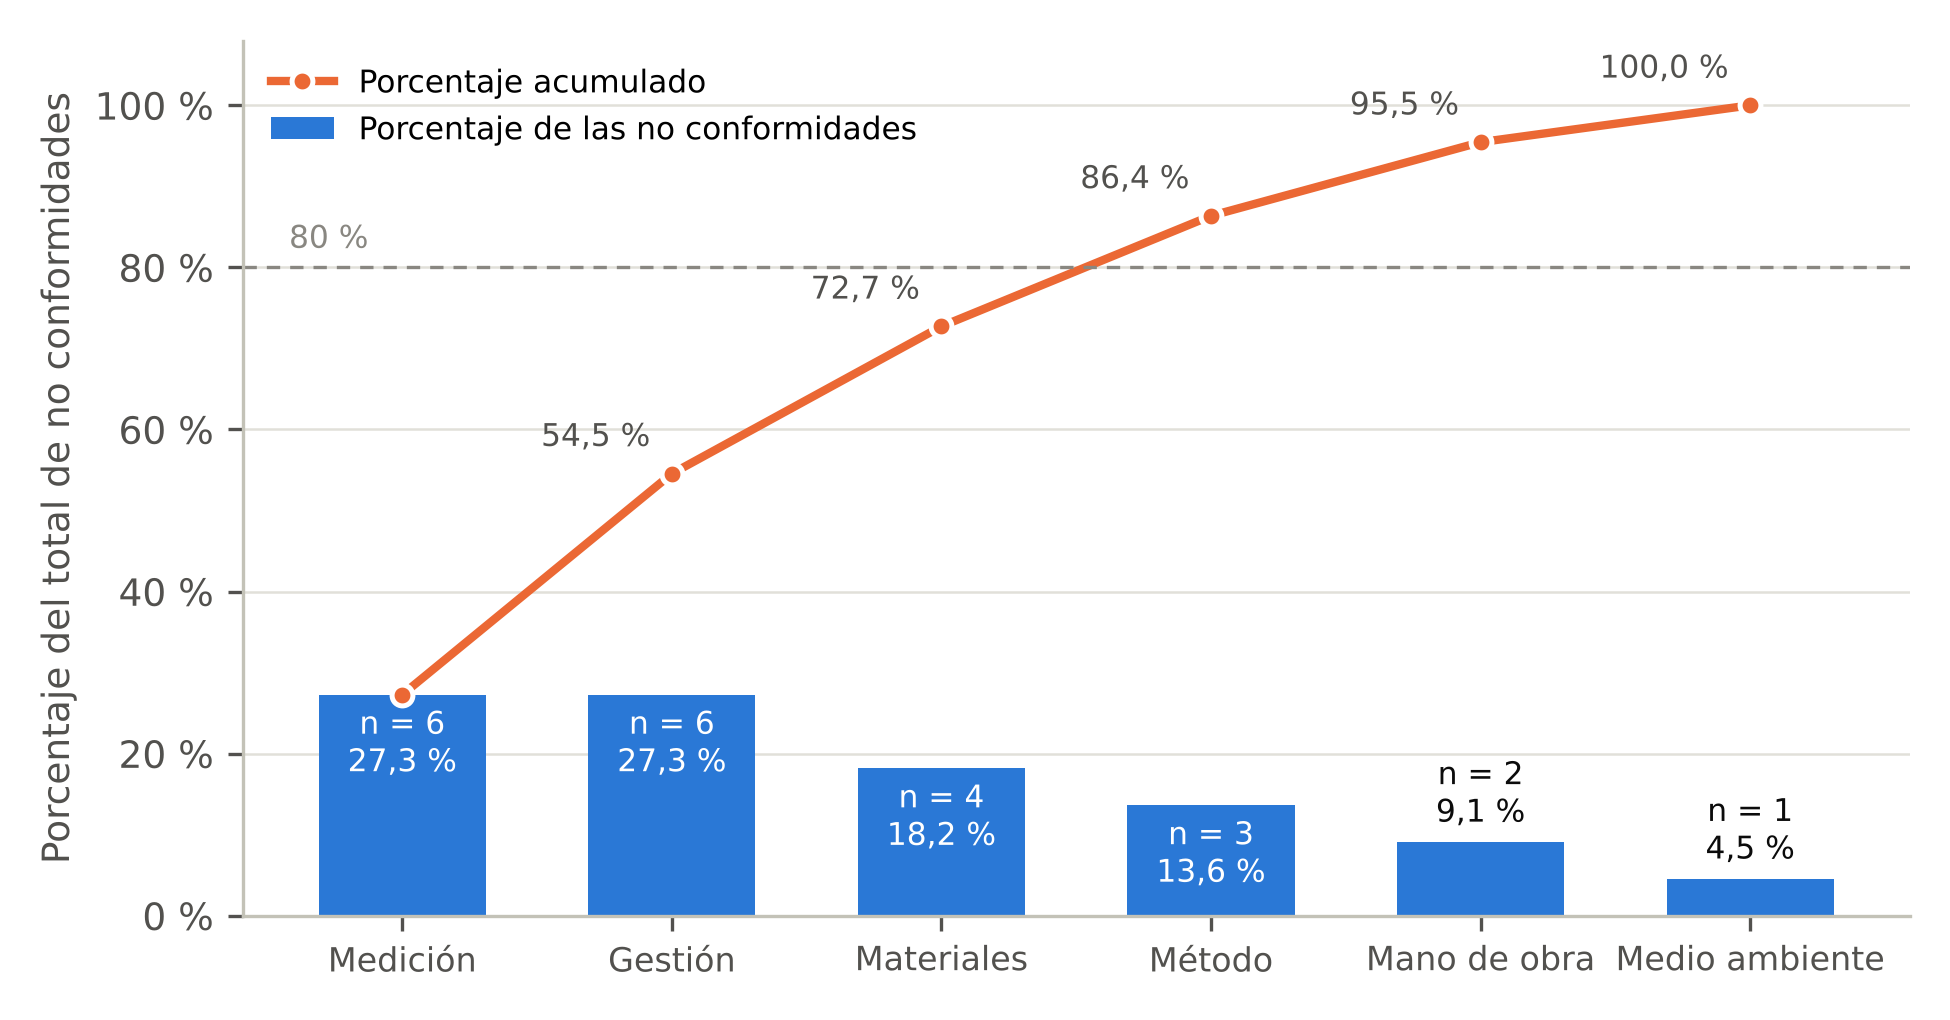
\includegraphics[width=\linewidth]{fig_pareto_nc}
\nota{Elaboración propia con los datos de la Tabla~\ref{tab:nc} ($n = 22$). Las barras indican el porcentaje de NC de cada categoría y la línea, el porcentaje acumulado; la línea discontinua marca el 80~\%. Figura generada con el script \texttt{cap2\_diagnostico\_figuras.py}.}
\end{figure}

\textbf{Diagrama de Ishikawa.} Las causas del desperdicio de materiales y de los sobrecostos de la losa se organizaron en un diagrama de causa y efecto (Figura~\ref{fig:ishikawa}). El efecto analizado es el costo adicional de la losa respecto de su costo teórico: materiales entregados por encima de lo necesario, hormigón y acero sin control de consumo, cantidades que hubo que corregir y riesgo de retrabajos por un hormigón no verificado.

\begin{figure}[H]
\centering
\caption{Diagrama de Ishikawa del desperdicio de materiales y los sobrecostos de la primera losa}
\label{fig:ishikawa}
\begin{tikzpicture}[
  font=\scriptsize,
  cat/.style={draw, rounded corners=2pt, fill=gray!12, font=\footnotesize\bfseries,
              inner sep=3pt, minimum width=3.6cm},
  lista/.style={align=left, text width=3.8cm, inner sep=2pt},
  espina/.style={-{Stealth[length=3.5mm]}, line width=1.4pt},
  rama/.style={-{Stealth[length=2.5mm]}, thick, black!75}]
  % Espina principal y efecto
  \draw[espina] (0,0) -- (12.55,0);
  \node[draw, thick, fill=gray!8, align=center, text width=3.0cm, minimum height=2.0cm,
        font=\footnotesize] (efecto) at (14.25,0)
        {\textbf{Desperdicio de materiales y sobrecostos} de la losa alivianada (primera losa)};
  % Ramas superiores
  \node[cat] (cMat) at (2.0,4.75) {Materiales};
  \node[lista, below=1pt of cMat] (lMat) {%
    -- Viguetas inexistentes en los tamaños requeridos; cambio sin registro\\
    -- Acero entregado en 30~\%; demoras por combustible\\
    -- EPS distinto de la ET; 2.350 piezas sin conciliar\\
    -- Certificados tardíos; sin $\phi$6, $\phi$10, cemento ni áridos};
  \node[cat] (cMet) at (6.1,4.75) {Método};
  \node[lista, below=1pt of cMet] (lMet) {%
    -- Sin plan de la calidad ni PPI\\
    -- Sin despiece ni pedido por paño; sin kardex ni vales\\
    -- Acopio sin recepción ni inventario\\
    -- Sin dosificación aprobada ni curado registrado; vaciado con carretillas};
  \node[cat] (cMO) at (10.2,4.75) {Mano de obra};
  \node[lista, below=1pt of cMO] (lMO) {%
    -- Competencia y capacitación no registradas\\
    -- Parrilla pisada y sin separadores visibles\\
    -- Supervisión apoyada por pasantes\\
    -- Presión por recuperar el retraso};
  % Ramas inferiores
  \node[lista, anchor=south] (lMed) at (2.0,-4.45) {%
    -- Losa sin probetas; pago antes de los 28 días\\
    -- Acero de la losa sin planilla de armado; factor 3 en el cierre\\
    -- Tres cifras del acero acumulado; correcciones posteriores\\
    -- Calidad «buena» sin evidencia objetiva};
  \node[cat, below=1pt of lMed] (cMed) {Medición};
  \node[lista, anchor=south] (lAmb) at (6.1,-4.45) {%
    -- Lluvias durante el armado (12, 13 y 21/11/2025)\\
    -- Bajas temperaturas a 3.650~m~s.~n.~m. sin plan de tiempo frío\\
    -- Escasez de diésel y alza de precios\\
    -- Contrato sin reajuste de precios};
  \node[cat, below=1pt of lAmb] (cAmb) {Medio ambiente};
  \node[lista, anchor=south] (lGes) at (10.2,-4.45) {%
    -- Libro de Órdenes sin NC ni constancia del Director\\
    -- Documentos incoherentes (ET, Plano~02, certificados)\\
    -- Cronograma desactualizado; riesgos no gestionados\\
    -- Sin registro de costos de la calidad};
  \node[cat, below=1pt of lGes] (cGes) {Gestión};
  % Conectores hacia la espina
  \foreach \l/\x in {lMat/3.35, lMet/7.45, lMO/11.55} {
    \draw[rama] (\l.south) -- (\x,0.05);
  }
  \foreach \l/\x in {lMed/3.35, lAmb/7.45, lGes/11.55} {
    \draw[rama] (\l.north) -- (\x,-0.05);
  }
\end{tikzpicture}
\nota{Elaboración propia con base en las no conformidades de la Tabla~\ref{tab:nc} y en el análisis documental de la Sección~\ref{sec:analisis-documental}. No se identificaron causas documentadas en la categoría de maquinaria.}
\end{figure}

El diagrama muestra que las causas se refuerzan entre sí. Las externas (escasez de combustible, falta de viguetas, alza de precios y lluvias) se convirtieron en problemas de la losa porque no había un sistema que las anticipara: sin plan de compras ni existencias mínimas, el desabastecimiento obligó a cambiar el diseño y a recibir materiales sin inspección; sin cantidades teóricas por paño, el excedente de materiales no pudo detectarse; y sin ensayos ni registros, la conformidad del hormigón y de las cantidades quedó sin demostrar. La causa raíz común es la falta de un sistema de gestión de la calidad del ítem: la calidad se confió a la verificación puntual de la Supervisión antes de cada vaciado, sin criterios escritos, registros ni seguimiento. Como el contrato no admite reajuste de precios y los precios unitarios incluyen la reparación de trabajos defectuosos \parencite[pp.~92, 95]{uatf2025pao2}, el costo de estas causas recae en el contratista; es la justificación económica del SGC que se diseña en la Sección~\ref{sec:diseno-sgc}.

% ---------------------------------------------------------------------
\subsection{Línea base cuantitativa}
\label{sec:linea-base-cuantitativa}

La línea base cuantitativa ($O_1$) expresa, para cada material, la cantidad teórica de la primera losa, la cantidad entregada y la pagada, el índice de desperdicio que puede documentarse y los parámetros con que el modelo representa el escenario de control (sin SGC). En ella se distinguen tres tipos de dato: \emph{hechos documentados}, que son las cantidades entregadas y pagadas con su fuente; \emph{cálculos propios} reproducibles, que son las cantidades teóricas y los índices calculados con ellas; y \emph{supuestos con fuente}, que se usan para los materiales sin registros de consumo.

\textbf{Cantidades teóricas.} Las cantidades teóricas se calcularon paño por paño con los planos 01 a 03 \parencite{uatf_planos}. Las 41 áreas del Plano~01 coinciden con las del cómputo. Las viguetas se contaron y midieron en el Plano~03, corrigiendo las etiquetas con el dibujo cuando no coincidían, y su longitud se tomó como la luz libre más 5~cm de apoyo en cada extremo, según el detalle de apoyo del Plano~02. Los complementos se contaron por filas entre viguetas, con la pieza suministrada de 20~$\times$~100~$\times$~44~cm. El hormigón es el volumen de la losa de 25~cm menos el de los complementos y el de las viguetas. El acero comprende la malla de $\phi$6~c/20~cm en ambas direcciones, con anclajes y traslapes, los negativos sobre los apoyos y los nervios transversales. Como ningún plano ubica los nervios ni define los negativos, el escenario base supone un nervio a media luz en los paños con luz libre media de 4,0~m o más y una barra de $\phi$8 por vigueta sobre cada apoyo continuo; con otros supuestos razonables, el acero teórico varía entre 2,72 y 3,44~kg/\mdos{}. La Tabla~\ref{tab:cantidades-teoricas} presenta los resultados; el cálculo por paño, sus supuestos y su análisis de sensibilidad se conservan en la carpeta de extracción de datos de obra del repositorio (\texttt{Cantidades\_Teoricas\_Primera\_Losa\_por\_Pano.csv} y \texttt{Metodo\_Cantidades\_Teoricas.md}).

\begin{table}[H]
\caption{Cantidades teóricas de materiales de la primera losa y del saldo}
\label{tab:cantidades-teoricas}
\setlength{\tabcolsep}{4pt}
\begin{tabularx}{\linewidth}{@{}P{2.75cm}P{2.6cm}P{2.45cm}P{2.55cm}L@{}}
\toprule
\textbf{Material} & \textbf{Primera losa (1.109,84~\mdos{})} & \textbf{Por \mdos{}} & \textbf{Saldo (2.234,60~\mdos{})} & \textbf{Supuestos principales} \\
\midrule
Viguetas pretensadas & 531 piezas; 2.205,1~m & 1,987~m (0,478 piezas) & 4.439,8~m & Longitud igual a la luz libre más 2~$\times$~0,05~m; etiquetas del Plano~03 corregidas con el dibujo \\
Complementos de EPS & 2.237,9 piezas & 2,016 piezas & 4.505,9 piezas & Piezas netas por fila; nervio a media luz si la luz es de 4,0~m o más (sin nervios: 2,048 piezas/\mdos{}) \\
Hormigón vaciado en obra & 79,31~\mtres{} & 0,0715~\mtres{} & 159,7~\mtres{} & Complemento de 0,20~m (el suministrado); vigueta de 17,2~kg/m según una ficha técnica de referencia \\
Acero & 3.572,8~kg & 3,22~kg (malla 2,42; negativos 0,30; nervios 0,50) & 7.193,6~kg & Rango de 2,72 a 3,44~kg/\mdos{} según la ubicación de los nervios y la cuantía de los negativos \\
\bottomrule
\end{tabularx}
\nota{Elaboración propia (cálculo propio) con base en los planos 01 a 03 \parencite{uatf_planos}, el certificado de los complementos \parencite{unicon2025} y la ficha de viguetas de \textcite{concretec2018viguetas}. El saldo resulta de multiplicar las cantidades por \mdos{} de la primera losa por 2.234,60~\mdos{}, porque los paños de la segunda y la tercera losa son homólogos (Sección~\ref{sec:poblacion}).}
\end{table}

\textbf{Cantidades entregadas, pagadas e índices documentados.} La Tabla~\ref{tab:linea-base} compara las cantidades teóricas con las entregadas y las pagadas. Solo dos materiales tienen un dato documental que permite calcular un índice: el EPS, por la cantidad entregada, y el acero, por la cantidad pagada.

\begin{table}[H]
\caption{Cantidades teóricas, entregadas y pagadas de la primera losa e índices de la línea base}
\label{tab:linea-base}
\setlength{\tabcolsep}{3.5pt}
\begin{tabularx}{\linewidth}{@{}P{1.9cm}P{2.3cm}P{2.3cm}P{2.9cm}LP{2.6cm}@{}}
\toprule
\textbf{Material} & \textbf{Teórico} & \textbf{Entregado} & \textbf{Pagado o medido} & \textbf{Índice de la línea base} & \textbf{Tipo de dato} \\
\midrule
Viguetas & 531 piezas; 2.205,1~m & Sin notas de entrega & Incluidas en el ítem~13 (1.109,84~\mdos{}) & No documentado & Supuesto del autor \\
EPS & 2.237,9 piezas & 2.350 piezas & Incluido en el ítem~13 & IDM = +5,01~\% (+112 piezas); entre +3,4 y +5,9~\% según los supuestos & Documentado y cálculo propio \\
Hormigón & 79,31~\mtres{} & Sin remisiones ni vales de cemento & Incluido en el ítem~13 & No documentado & Supuesto de literatura \\
Acero & 3.572,8~kg (3,22~kg/\mdos{}) & Sin registro de entregas para la losa & 4.171,18~kg (3,76~kg/\mdos{}) en el ítem~8; 3~$\times$~4.171,18~kg en el cómputo de cierre & Pagado frente a teórico: +16,75~\%; entre +9,2 y +38,3~\% según los supuestos & Documentado y cálculo propio (aproximación del IDM) \\
\bottomrule
\end{tabularx}
\nota{Elaboración propia con base en la Tabla~\ref{tab:cantidades-teoricas}, \textcite{unicon2025}, \textcite[pp.~16, 19--20]{uatf2025pao2} y \textcite[hoja «Cómputos métricos», fila 538]{uatf_pao3}. IDM: ecuación~\eqref{eq:idm}.}
\end{table}

En el EPS se entregaron 2.350 piezas frente a 2.237,9 teóricas: 112 piezas más, es decir, un IDM de +5,01~\% (cálculo propio). Si no se construyeran nervios, el índice sería de +3,4~\%, y con la regla simplificada de dos piezas por \mdos{}, de +5,9~\%. Si cada fila se completara con piezas enteras, sin reaprovechar los recortes, se necesitarían unas 2.476 piezas, más que las entregadas; la cantidad recibida solo alcanza si los recortes se reaprovecharon, lo que es compatible con un desperdicio de 3~\% a 6~\% sobre el consumo neto. El índice supone que todas las piezas se destinaron a la primera losa y que no hubo devoluciones ni sobrantes, lo que no puede verificarse sin notas de entrega ni kardex.

En el acero, la única cantidad documentada de la losa es la pagada en la Planilla N.\textsuperscript{o}~2: 4.171,18~kg, es decir, 3,76~kg/\mdos{}, un 16,75~\% más que la cantidad teórica del escenario base (cálculo propio). La cantidad pagada supera la teórica con todos los supuestos ensayados: de +9,2~\% si se colocaran nervios en todas las luces de 3~m o más, a +38,3~\% si no hubiera nervios. La documentación no permite separar en esa diferencia el desperdicio real (recortes y traslapes no previstos), una medición superior a la ejecutada o armaduras que los planos no definen; por eso el índice se usa como una aproximación del desperdicio de acero de la línea base, no como una medición directa. El valor coincide con los desperdicios de 14,58~\% y 17,09~\% que \textcite[pp.~147, 169]{chino2024} midieron con el método convencional de habilitado del acero. La cifra de 12.513,54~kg del cómputo de cierre, 3,5 veces la cantidad teórica de una losa, no se usó, porque no corresponde a una losa ejecutada (Sección~\ref{sec:analisis-documental}).

Para las viguetas y el hormigón no existen notas de entrega, remisiones, vales de cemento ni volúmenes por vaciado, por lo que su desperdicio en la primera losa no puede medirse. Para el hormigón se adoptó el rango de la literatura: 5~\% como valor típico y hasta 22~\% en obras sin control volumétrico \parencite[pp.~53, 73]{galarza2011}, pérdidas reales de 14~\% a 27~\% en vaciados semanales sin control \parencite[pp.~33, 40]{rojas2018} y de 1,5~\% a 13~\% para el hormigón premezclado en Brasil \parencite[p.~106]{maciel2016}. Para las viguetas, que se fabrican a medida según el Plano~03, se supuso un desperdicio pequeño por rotura en la manipulación. Tampoco hay registros de retrabajos en la primera losa (NC-11), lo que no prueba que no los hubiera; su costo se representó como una fracción del costo directo tomada de la literatura: fallas visibles de 2,34~\% del costo total en 25 proyectos \parencite[p.~5421]{khadim2023}, costos de no calidad de 2,7~\% a 5,1~\% en la partida de hormigón armado \parencite[p.~1]{gudiel2020} y reprocesos de 6,5~\% en proyectos sin SGC \parencite[p.~12]{alvarez2014}.

\textbf{Parámetros del escenario de control.} La Tabla~\ref{tab:parametros-linea-base} resume los parámetros de la línea base que usa el modelo, con distribuciones triangulares (mínimo, moda y máximo). La tabla completa, con las eficacias del SGC y sus costos, está en el Anexo~\ref{anx:modelo}.

\begin{table}[H]
\caption{Parámetros de la línea base (escenario de control) del modelo de costos}
\label{tab:parametros-linea-base}
\setlength{\tabcolsep}{3.5pt}
\begin{tabularx}{\linewidth}{@{}P{2.7cm}Q{1.55cm}Q{1.55cm}Q{1.55cm}P{2.5cm}L@{}}
\toprule
\textbf{Parámetro} & \textbf{Mínimo} & \textbf{Moda} & \textbf{Máximo} & \textbf{Tipo de dato} & \textbf{Fuente} \\
\midrule
IDM de las viguetas & 0,0~\% & \IDMsinVig & 3,0~\% & Supuesto del autor & Viguetas fabricadas a medida; rotura en la manipulación \\
IDM del EPS & 2,5~\% & \IDMsinEps & 7,5~\% & Documentado (moda); rango supuesto de $\pm$50~\% & 2.350 piezas entregadas frente a 2.237,9 teóricas \\
IDM del hormigón & 5,0~\% & \IDMsinHor & 22,0~\% & Literatura & \textcite{galarza2011}; \textcite{rojas2018}; \textcite{maciel2016} \\
IDM del acero & 7,0~\% & \IDMsinAce & 26,0~\% & Documentado (moda); rango de literatura & 4.171,18~kg pagados frente a 3.572,8~kg teóricos; \textcite{galarza2011}; \textcite{maciel2016} \\
Retrabajo ($\rho$), fracción del costo directo & 0,5~\% & 2,34~\% & 6,5~\% & Literatura & \textcite{khadim2023}; \textcite{gudiel2020}; \textcite{alvarez2014} \\
\bottomrule
\end{tabularx}
\nota{Elaboración propia con los parámetros del modelo (archivo \texttt{parametros.json}, Anexo~\ref{anx:modelo}). Las páginas de las fuentes se indican en el texto. IDM: índice de desperdicio de materiales.}
\end{table}

\textbf{Costo de no calidad de la línea base.} Los materiales se valoraron con el análisis de precios unitarios de referencia, calibrado al precio del contrato (Anexo~\ref{anx:apu}). El costo teórico por \mdos{} de los materiales de la losa es de Bs~\CostoVig{} para las viguetas, Bs~\CostoEps{} para el EPS, Bs~\CostoHor{} para el hormigón y Bs~\CostoAce{} para el acero, en total Bs~\CMteo/\mdos{}, dentro de un costo directo teórico de Bs~\CDteo/\mdos{}. Con los valores más probables de los parámetros, el desperdicio ponderado por el costo de los materiales ---el IDM ponderado--- es de \IDMsinDet{}, y el costo de no calidad, que suma el desperdicio valorado y los retrabajos, es de Bs~\CNCsinDet/\mdos{}, el \CNCsinDetPct{} del costo unitario sin SGC (Bs~\CUsinDet/\mdos{}). Estos valores son la referencia $O_1$ de las hipótesis específicas: el escenario de control repite este desempeño en el saldo de 2.234,60~\mdos{}. Las distribuciones de probabilidad de estos indicadores y su comparación con el escenario con SGC se presentan en el Capítulo~\ref{cap:resultados}.

Las cantidades teóricas por paño también son la base del control que propone el SGC: con ellas se emite la lista de materiales de cada paño antes de ejecutarlo y se concilian las cantidades entregadas, colocadas, medidas y pagadas (Sección~\ref{sec:sgc-operacion}). En la primera losa ese control no existió, y por eso solo dos de los cuatro materiales tienen una línea base documentada. \pendiente{completar la línea base con las notas de entrega de PRETENSA y UNICON, los vales de cemento y los volúmenes por vaciado, si la Supervisión o la contratista los facilitan; con ellos se recalcularán los IDM de las viguetas y del hormigón.}
}{}
\IfFileExists{capitulos_sencilla/31_capitulo2_sgc.tex}{% =====================================================================
%  CAPÍTULO 2 (continuación). 2.6 DISEÑO DEL SISTEMA DE GESTIÓN DE LA
%  CALIDAD: propuesta de la tesis (variable independiente X).
%  Cada componente responde a una brecha del diagnóstico (B1 a B9) y se
%  resume en la matriz de trazabilidad (Tabla tab:trazabilidad).
%  Formatos completos: Anexo C (capitulos/91_anexo_instrumentos.tex).
% =====================================================================
\section{Diseño del Sistema de Gestión de la Calidad}
\label{sec:diseno-sgc}

Esta sección presenta la propuesta central de la tesis: el Sistema de Gestión de la Calidad (SGC) para el proceso constructivo de las losas alivianadas con viguetas pretensadas del Edificio de Posgrado. El sistema corresponde a la variable independiente ($X$) del modelo de investigación y se diseñó a partir de las brechas de la línea base, es decir, de la ejecución de la primera losa (41 paños; 1.109,84~\mdos{}) sin un sistema formal de gestión de la calidad (Sección~\ref{sec:analisis-documental}). Las nueve brechas que el sistema debe cerrar agrupan las 22 no conformidades del diagnóstico (Tabla~\ref{tab:nc}):

\begin{enumerate}[label=\textbf{B\arabic*.},leftmargin=1.3cm]
  \item \textbf{Hormigón sin control.} Ninguna probeta de la losa; las de columnas y vigas, elaboradas por la contratista, se ensayaron a 55--76 días y se «proyectaron» a 28 días \parencite{labuatf2025}; no hay registros de dosificación, asentamiento, vaciado ni curado \parencite[p.~76]{uatf2025pao2}. La losa se certificó para pago sin resultados de resistencia: los 28 días desde la autorización del vaciado (28/11/2025) vencían el 26/12/2025, después del cierre de la planilla N.\textsuperscript{o}~2 (08/12/2025) (cálculo propio).
  \item \textbf{Evidencias pedidas o posteriores al uso.} La Supervisión tuvo que pedir garantías, roturas de probetas y dosificaciones \parencite[p.~9]{uatf2025pao2}. Los certificados de viguetas y de EPS, sin firma, son del 27/11/2025, con la losa en armado desde el 14/11/2025; el de viguetas no indica cantidad, lote ni ensayos; no hay certificado del acero $\phi$6 ni del $\phi$10 \parencite[pp.~80--86, 122]{uatf2025pao2}.
  \item \textbf{Documentos incoherentes.} El complemento EPS mide 100~$\times$~50~$\times$~20~cm en la especificación técnica (ET), 0,15~m de altura en el Plano~02 y 20~$\times$~100~$\times$~44~cm en el certificado; la ET cita la CBH-87 y normas antiguas de cemento, áridos y agua \parencite[pp.~1--3]{uatf_et}.
  \item \textbf{Cantidades sin conciliar.} Al cierre se descontaron 1.915,16~kg de acero ($-$3,65~\%); el acero de la losa figura 1,00 vez en la planilla N.\textsuperscript{o}~2 y «3~$\times$~4.171,18~kg» en el cómputo de cierre, y la ET del ítem~13 incluye la parrilla y los negativos: inconsistencias (posible doble cómputo) que deben verificar la Supervisión y la Fiscalización; el acumulado de acero difiere entre documentos (52.424,65; 50.509,49 y 50.561,84~kg) \parencites[pp.~19--20]{uatf2025pao2}{uatf_pao3}[p.~12]{uatf_item13}.
  \item \textbf{Consumos sin registro.} No hay kardex, vales ni remisiones; se entregaron 2.350 piezas de EPS frente a $\approx$~2.220 teóricas, sin descontar nervios ni bordes \parencite{unicon2025}.
  \item \textbf{Sin PPI ni liberación.} El 28/11/2025 la contratista pidió verificar el armado y la Supervisión autorizó el vaciado el mismo día, sin pedir probetas; las ocho solicitudes de vaciado del periodo se autorizaron en el día \parencite[pp.~114--125]{uatf2025pao2}. Las fotografías muestran la parrilla pisada y sin separadores visibles \parencite[p.~76]{uatf2025pao2}.
  \item \textbf{Sin no conformidades ni costos de la calidad.} Ninguno de los 24 asientos del Libro de Órdenes registra una no conformidad o un retrabajo, y en ninguna hoja firma el Director de obra \parencite[pp.~114--125]{uatf2025pao2}.
  \item \textbf{Suministro y precios.} Escasez de diésel, paralización de FANCESA, entrega del 30~\% del acero pedido, demoras por falta de combustible y falta de viguetas de los tamaños requeridos \parencites{fancesa2025,laslomas2025}[pp.~11, 123]{uatf2025pao2}; alza de precios reconocida por decretos de ajuste \parencite{ds5321_2025,ds5597_2026}.
  \item \textbf{Clima.} Siete días de lluvia notificados entre septiembre y noviembre de 2025, tres durante el armado de vigas y losa \parencite[pp.~114--124]{uatf2025pao2}, y riesgo de heladas a 3.650~m~s.~n.~m.
\end{enumerate}

El diseño se desarrolla en diez bloques: enfoque y estructura del sistema (Sección~\ref{sec:sgc-enfoque}); contexto y alcance (Sección~\ref{sec:sgc-contexto}); liderazgo (Sección~\ref{sec:sgc-liderazgo}); planificación (Sección~\ref{sec:sgc-planificacion}); apoyo (Sección~\ref{sec:sgc-apoyo}); operación (Sección~\ref{sec:sgc-operacion}); evaluación del desempeño (Sección~\ref{sec:sgc-evaluacion}); mejora (Sección~\ref{sec:sgc-mejora}); costos de la calidad (Sección~\ref{sec:sgc-costos}), y matriz de trazabilidad entre brechas, requisitos, componentes e indicadores (Sección~\ref{sec:sgc-trazabilidad}). Los formatos para aplicar el sistema en obra se presentan completos en el Anexo~\ref{anx:instrumentos}.

% ---------------------------------------------------------------------
\subsection{Enfoque y estructura del sistema}
\label{sec:sgc-enfoque}

El SGC propuesto es un \emph{sistema de gestión de la calidad del proyecto}: no busca certificar a una empresa, sino asegurar que la ejecución del ítem~13 en los 2.234,60~\mdos{} pendientes cumpla los requisitos con el menor desperdicio posible. Por ello se concreta en un \emph{plan de la calidad del ítem}, elaborado con las directrices de la norma ISO~10005:2018 para planes de la calidad de un proyecto o contrato específico \parencite{iso10005_2018}, y organizado sobre la estructura de cláusulas 4 a 10 de la norma ISO~9001:2026 \parencite{iso9001_2026}. Cada cláusula se desarrolla en un bloque: contexto (4) en la Sección~\ref{sec:sgc-contexto}; liderazgo (5) en la \ref{sec:sgc-liderazgo}; planificación (6) en la \ref{sec:sgc-planificacion}; apoyo (7) en la \ref{sec:sgc-apoyo}; operación (8) en la \ref{sec:sgc-operacion}; evaluación del desempeño (9) en la \ref{sec:sgc-evaluacion}; y mejora (10) en las \ref{sec:sgc-mejora} y \ref{sec:sgc-costos}. Los números de cláusula citados corresponden a la estructura que la edición de 2026 conserva de la de 2015; las descripciones de los requisitos son paráfrasis del autor y no reproducen el texto de la norma. \pendiente{contrastar cada referencia de cláusula con la NB/ISO~9001:2026 adquirida en IBNORCA \parencite{ibnorca9001_2026}.}

El sistema lo aplica la empresa que ejecute la segunda y la tercera losa, que es quien compra, almacena, coloca y vacía los materiales; la UATF, por medio de la Supervisión y la Fiscalización, lo exige, lo aprueba y verifica su cumplimiento. Por ello se recomienda incorporar el plan de la calidad, el plan de puntos de inspección y ensayo (PPI) y los formatos del Anexo~\ref{anx:instrumentos} en las especificaciones del documento base de contratación del saldo de la obra, para que su cumplimiento sea una obligación contractual. El sistema funciona según el ciclo Planificar--Hacer--Verificar--Actuar (PHVA), aplicado a cada paño y a cada losa (Figura~\ref{fig:phva}); como la segunda y la tercera losa repiten la geometría de la primera, cada vuelta del ciclo aprovecha las lecciones de la anterior.

\begin{figure}[H]
\centering
\caption{Ciclo PHVA aplicado a la ejecución de la losa alivianada}
\label{fig:phva}
\begin{tikzpicture}[
  fase/.style={draw, rounded corners=3pt, thick, align=left, text width=5.9cm,
               minimum height=3.1cm, font=\footnotesize, inner sep=5pt},
  extremo/.style={draw, rounded corners=2pt, align=center, text width=12.6cm,
               font=\footnotesize, fill=gray!8, inner sep=4pt},
  flecha/.style={-{Stealth[length=3mm]}, very thick, black!70}]
  \node[fase, fill=blue!6]   (P) at (-4.1, 2.45)  {\textbf{P --- Planificar} (cláusulas 4 a 7)\\[2pt]
     -- Contexto, partes interesadas y alcance\\
     -- Política, objetivos e indicadores (IDM, \%CNC)\\
     -- Riesgos de suministro, precios y clima\\
     -- Plan de la calidad, PPI y procedimientos\\
     -- Capacitación del personal};
  \node[fase, fill=green!7]  (H) at (4.1, 2.45)   {\textbf{H --- Hacer} (cláusula 8)\\[2pt]
     -- Compra y recepción de materiales (PCM-01)\\
     -- Almacén y despacho por paño (PCM-02, PCM-03)\\
     -- Apuntalamiento, viguetas, EPS y armado\\
     -- Vaciado, muestreo y curado del hormigón\\
     -- Registro en fichas y vales};
  \node[fase, fill=orange!9] (V) at (4.1, -2.45)  {\textbf{V --- Verificar} (cláusula 9)\\[2pt]
     -- Liberación del paño en los puntos de espera\\
     -- Conciliación de cantidades (PCM-04)\\
     -- Ensayos a 28 días (ACI~318-25)\\
     -- Indicadores, auditoría y revisión mensual\\
     -- Conciliación con la planilla de avance};
  \node[fase, fill=red!6]    (A) at (-4.1, -2.45) {\textbf{A --- Actuar} (cláusula 10)\\[2pt]
     -- No conformidades y acción correctiva\\
     -- Análisis de causas (5 porqués, Ishikawa)\\
     -- Costos de la calidad (modelo PAF)\\
     -- Ajuste de metas y procedimientos\\
     -- Lecciones aprendidas para la losa siguiente};
  \node[circle, draw, very thick, fill=white, align=center, minimum size=2.0cm,
        font=\scriptsize] (C) at (0,0) {\textbf{Liderazgo}\\(cláusula 5)\\política de\\la calidad};
  \draw[flecha] (P.east) -- (H.west);
  \draw[flecha] (H.south) -- (V.north);
  \draw[flecha] (V.west) -- (A.east);
  \draw[flecha] (A.north) -- (P.south);
  \node[extremo, above=0.45cm of $(P.north)!0.5!(H.north)$] (E)
     {\textbf{Entradas:} requisitos de la UATF y de las partes interesadas (contrato, ET, planos 01 a 03, certificados, ACI~318-25, NB~997) y brechas de la primera losa (B1 a B9)};
  \node[extremo, below=0.45cm of $(A.south)!0.5!(V.south)$] (S)
     {\textbf{Salidas:} paños liberados y losa conforme; cantidades conciliadas, medidas y pagadas sin diferencias; menor desperdicio y menor costo unitario};
  \draw[flecha] (E.south) -- ++(0,-0.4);
  \draw[flecha] ($(S.north)+(0,0.4)$) -- (S.north);
\end{tikzpicture}
\nota{Elaboración propia. IDM: índice de desperdicio de materiales; \%CNC: costo de no calidad en porcentaje del costo del ítem; PCM: procedimiento de control de materiales; PAF: prevención, evaluación y fallas.}
\end{figure}

% ---------------------------------------------------------------------
\subsection{Contexto, partes interesadas, alcance y exclusiones}
\label{sec:sgc-contexto}

\textbf{Cuestiones externas e internas.} Las cuestiones externas pertinentes son la escasez de combustible, que paralizó temporalmente la producción de cemento y retrasó la entrega del acero \parencite{fancesa2025,laslomas2025}; el alza de precios de los materiales \parencite{ds5597_2026}; la falta de viguetas de los tamaños requeridos \parencite[p.~11]{uatf2025pao2}; el clima, con lluvias y bajas temperaturas, coherente con la atención que la edición vigente de la norma presta al cambio climático \parencite{iso9001_2026}; y la normativa de contratación pública. Las internas son la ausencia de registros de consumos, de inspección y de no conformidades; la dependencia de la experiencia del capataz; la información técnica incoherente; y el cambio de contratista para el saldo de la obra. Estas cuestiones se traducen en los riesgos de la Tabla~\ref{tab:riesgos}.

\textbf{Requisitos contractuales.} El contrato fija reglas que el SGC operativiza: los materiales se inspeccionan y ensayan antes de su incorporación, a costa de la contratista (cláusula 26.6), y se acopian en zonas aprobadas (26.9); el control de calidad es responsabilidad directa de la Supervisión (26.3); cada orden del Libro de Órdenes lleva la constancia firmada del Director de obra (25.ª); y las obras se miden netas, sin medir excedentes no aprobados por escrito (27.ª) \parencite[pp.~99--102]{uatf2025pao2}. Como los precios unitarios incluyen las reparaciones por trabajos defectuosos \parencite[p.~92]{uatf2025pao2}, el desperdicio y el retrabajo los absorbe la contratista, que tiene así un incentivo directo para aplicar el sistema.

\textbf{Partes interesadas.} La Tabla~\ref{tab:partes-interesadas} identifica a las partes interesadas pertinentes, sus necesidades y expectativas y el requisito que cada una genera para el SGC.

\begingroup\footnotesize\setstretch{1}\setlength{\tabcolsep}{4pt}
\begin{longtable}{@{}P{3.2cm}P{5.6cm}P{6.9cm}@{}}
\caption{Partes interesadas, necesidades y requisitos para el SGC}\label{tab:partes-interesadas}\\
\toprule
\textbf{Parte interesada} & \textbf{Necesidades y expectativas} & \textbf{Requisito que genera para el SGC} \\
\midrule
\endfirsthead
\multicolumn{3}{@{}l}{\textit{(continuación)}}\\
\toprule
\textbf{Parte interesada} & \textbf{Necesidades y expectativas} & \textbf{Requisito que genera para el SGC} \\
\midrule
\endhead
\bottomrule
\endfoot
UATF (propietaria; Departamento de Infraestructura) & Losa conforme a la ET y a los planos, en plazo y dentro del presupuesto; pagar solo lo ejecutado; uso transparente de recursos del IDH & Liberación documentada de cada paño; conciliación de cantidades antes de cada planilla; informe mensual de calidad \\
Fiscal de obra (UATF) & Control del avance físico y financiero y de las modificaciones del contrato & Trazabilidad de cantidades desde el plano hasta el pago; cambios documentados y aprobados antes de ejecutarse \\
Supervisor de obra & Verificar el trabajo antes de cada vaciado; contar con certificados, dosificaciones y ensayos sin tener que pedirlos (B2) & Puntos de espera del PPI; expediente de calidad al día; muestreo del hormigón por personal independiente de la producción \\
Contratista (Director de obra y personal) & Ejecutar sin retrabajos, paralizaciones ni descuentos; reglas de aceptación claras; cobro oportuno & Criterios de aceptación definidos de antemano; formatos simples; control del desperdicio, que es ahorro propio \\
Proyectista estructural (por medio de la UATF) & Que la losa se ejecute según el diseño: altura del complemento, armaduras, recubrimientos y apoyos & Consulta técnica y aprobación de los cambios; resolución de la discrepancia del complemento EPS (B3) \\
Proveedores de viguetas y de complementos (PRETENSA, UNICON) & Pedidos exactos por tipo, longitud y cantidad; manipulación y montaje según sus instrucciones & Pedido por paño según el Plano~03; recepción con criterios conocidos; cumplimiento de los pasos de montaje que exige el fabricante \parencite[p.~8]{uatf_item13} \\
Proveedores de acero, cemento y áridos & Pedidos programados; condiciones de entrega en un mercado con escasez de combustible & Plan de compras anticipado y existencia mínima; certificado por colada (acero) y por lote (cemento) \\
Laboratorio de ensayos & Muestras representativas, bien elaboradas, identificadas y curadas & Muestreo según ASTM~C172 y C31 por técnico competente; codificación de probetas por paño y vaciado \\
Usuarios del edificio (comunidad de posgrado) & Estructura segura y durable, sin fisuras ni flechas excesivas & Aceptación del hormigón según ACI~318-25; curado y desapuntalamiento controlados \\
Órganos de control gubernamental y sociedad & Uso transparente y verificable de recursos públicos & Registros auditables y comportamiento ético en la medición y el pago de cantidades \\
\end{longtable}
\vspace{-6pt}
\nota{Elaboración propia con base en los documentos del caso \parencite{uatf2025pao2,uatf_item13,uatf_et}. B2 y B3: brechas de la línea base.}
\endgroup

\textbf{Alcance y exclusiones.} El SGC comprende la planificación, el abastecimiento (compra, recepción, almacenamiento y despacho), la ejecución (apuntalamiento, viguetas y complementos, nervios, armaduras, instalaciones embebidas, hormigonado, curado y desapuntalamiento), el control de calidad (inspección, ensayos y liberación) y la medición, conciliación y pago del ítem~13 en la segunda y la tercera losa: 2.234,60~\mdos{}, $\approx$~1.117,30~\mdos{} por losa \parencite{uatf_pao3}. Incluye todo el acero colocado en la losa (parrilla, nervios y negativos), se pague por el ítem~8 o por el 13, para no dejar vacíos entre ítems (B4), y el muestreo de cada vaciado completo, incluidas las vigas que se vacían monolíticamente con la losa \parencite[p.~3]{uatf_et}. Se excluyen el diseño estructural (diseño y desarrollo, cláusula 8.3), que corresponde al proyectista de la UATF y del que el SGC solo gestiona las consultas y los cambios; la fabricación de viguetas y complementos, que se controla como suministro externo mediante certificados e inspección de recepción; y los demás ítems de la obra. Estas exclusiones no afectan la capacidad del sistema para asegurar la conformidad de la losa.

% ---------------------------------------------------------------------
\subsection{Liderazgo: política de la calidad, organización y responsabilidades}
\label{sec:sgc-liderazgo}

\textbf{Política de la calidad del proyecto.} La política expresa el compromiso de la dirección de obra y sirve de marco para los objetivos de la Sección~\ref{sec:sgc-planificacion}. Se propone el siguiente texto, que debe firmar el Director de obra, contar con el visto bueno de la Supervisión y exhibirse en la oficina y en el almacén de la obra:

\begin{center}
\fcolorbox{gray!60}{gray!6}{\parbox{0.92\linewidth}{\setstretch{1.15}\small
\textbf{Política de la calidad de la ejecución de las losas alivianadas del Edificio de Posgrado (UATF)}\par\smallskip
La dirección de obra se compromete a:
\begin{enumerate*}[label=(\arabic*)]
  \item ejecutar cada paño conforme a los planos aprobados, a las especificaciones técnicas y al código ACI~318-25, sin vaciar ningún paño que no haya sido liberado;
  \item controlar cada material desde la compra hasta su colocación, para consumir y pagar solo lo necesario y reducir el desperdicio;
  \item medir y cobrar las cantidades con evidencia verificable, con honestidad y transparencia en el uso de los recursos públicos;
  \item anticipar los riesgos de suministro, de precios y de clima;
  \item registrar, corregir y analizar las no conformidades para mejorar de forma continua; y
  \item capacitar al personal y comunicar oportunamente la información de la calidad a la Supervisión y a la Fiscalización.
\end{enumerate*}}}
\end{center}

\textbf{Organización.} En la contratista, el Director de obra es el responsable del SGC: aprueba el plan, asigna los recursos y preside la revisión mensual; el Residente de obra actúa como encargado de calidad (en una obra de este tamaño, con tiempo asignado para inspeccionar, registrar y conciliar); el Almacenero administra el kardex y los vales; y el Capataz dirige a los armadores y ejecuta el autocontrol. Por la UATF, el Supervisor de obra verifica y libera los paños, y el Fiscal de obra controla el contrato, las planillas y las modificaciones. El laboratorio y los proveedores son externos; el laboratorio entrega los informes de ensayo a la Supervisión y a la contratista \parencite[sección 26.12.1.1, p.~602]{aci318_2025}.

\textbf{Matriz de responsabilidades.} La Tabla~\ref{tab:raci} asigna las responsabilidades con la notación RACI: \textbf{R}, ejecuta la actividad; \textbf{A}, aprueba y rinde cuentas por ella (una sola por actividad); \textbf{C}, es consultado antes de decidir; e \textbf{I}, es informado del resultado.

\begingroup\footnotesize\setstretch{1}\setlength{\tabcolsep}{3pt}
\begin{longtable}{@{}P{6.1cm}*{8}{Q{0.98cm}}@{}}
\caption{Matriz de responsabilidades (RACI) del SGC del ítem losa alivianada}\label{tab:raci}\\
\toprule
\textbf{Actividad} & \textbf{DO} & \textbf{RC} & \textbf{AL} & \textbf{CA} & \textbf{LB} & \textbf{SU} & \textbf{FI} & \textbf{PR} \\
\midrule
\endfirsthead
\multicolumn{9}{@{}l}{\textit{(continuación)}}\\
\toprule
\textbf{Actividad} & \textbf{DO} & \textbf{RC} & \textbf{AL} & \textbf{CA} & \textbf{LB} & \textbf{SU} & \textbf{FI} & \textbf{PR} \\
\midrule
\endhead
\bottomrule
\endfoot
1. Elaborar el plan de la calidad, el PPI y los procedimientos & A & R & C & C & C & I & I & -- \\
2. Revisar y aprobar el plan de la calidad, el PPI y la dosificación del hormigón & I & C & -- & -- & C & A & I & -- \\
3. Planificar las compras y evaluar a los proveedores & A & R & C & -- & -- & I & -- & C \\
4. Recibir, inspeccionar, almacenar y registrar materiales (PCM-01 y PCM-02) & I & A & R & -- & -- & I & -- & C \\
5. Despachar materiales por paño con vales (PCM-03) & -- & A & R & R & -- & -- & -- & -- \\
6. Ejecutar apuntalamiento, viguetas, EPS, armado e instalaciones & I & A & -- & R & -- & I & -- & C \\
7. Inspeccionar y liberar el paño en los puntos de espera & I & R & -- & C & -- & A & I & -- \\
8. Dosificar, mezclar, vaciar, vibrar y curar el hormigón; desapuntalar & I & A & C & R & C & I & -- & -- \\
9. Muestrear el hormigón, elaborar y ensayar las probetas e informar & I & C & -- & -- & R & A & I & -- \\
10. Conciliar cantidades por paño y por planilla (PCM-04) & A & R & C & C & -- & C & I & -- \\
11. Revisar y aprobar la planilla de avance & C & C & -- & -- & -- & R & A & -- \\
12. Tratar el material no conforme y las no conformidades (PCM-05; acción correctiva) & A & R & C & C & C & C & I & C \\
13. Registrar los costos de la calidad (PAF) & A & R & C & -- & -- & -- & I & -- \\
14. Atender consultas técnicas (p.~ej., complemento EPS) & C & R & -- & -- & -- & A & I & C \\
15. Aprobar órdenes de cambio o modificaciones con efecto en cantidades o monto & C & C & -- & -- & -- & R & A & -- \\
16. Reunión semanal de calidad y revisión mensual & A & R & C & C & -- & C & I & -- \\
17. Auditoría interna simplificada & A & C & C & C & -- & R & I & -- \\
\end{longtable}
\vspace{-6pt}
\nota{Elaboración propia. DO: Director de obra; RC: Residente de obra y encargado de calidad; AL: Almacenero; CA: Capataz y armadores; LB: laboratorio de ensayos; SU: Supervisor de obra; FI: Fiscal de obra; PR: proveedores. En la auditoría interna, el responsable de ejecutarla (R) puede ser el Supervisor o un profesional independiente del proceso auditado, designado de común acuerdo.}
\endgroup

% ---------------------------------------------------------------------
\subsection{Planificación: riesgos, oportunidades y objetivos de la calidad}
\label{sec:sgc-planificacion}

\textbf{Método de valoración de riesgos.} Cada riesgo del proceso de la losa se valoró con una probabilidad $P$ y un impacto $I$ en una escala de tres niveles. La probabilidad es baja (1) si no hay antecedentes en la obra, media (2) si el hecho es posible por las condiciones de la obra y alta (3) si ya ocurrió en la primera losa o en el periodo de ejecución. El impacto es bajo (1) si solo genera una corrección menor, medio (2) si causa desperdicio, retrabajo o un retraso de días, y alto (3) si compromete la seguridad estructural, el pago correcto de cantidades o la continuidad de la obra. El nivel de riesgo es $N = P \times I$: bajo de 1 a 2, medio de 3 a 4 y alto de 6 a 9. Todo riesgo alto debe tener un control obligatorio en un procedimiento o en el PPI, un indicador y un responsable. La Tabla~\ref{tab:riesgos} presenta la matriz resultante.

\begingroup\footnotesize\setstretch{1}\setlength{\tabcolsep}{3pt}
\begin{longtable}{@{}P{0.75cm}P{3.25cm}P{3.85cm}Q{0.45cm}Q{0.45cm}Q{0.6cm}P{5.75cm}@{}}
\caption{Matriz de riesgos del proceso constructivo de la losa alivianada}\label{tab:riesgos}\\
\toprule
\textbf{N.\textsuperscript{o}} & \textbf{Riesgo} & \textbf{Causa o evidencia} & \textbf{$P$} & \textbf{$I$} & \textbf{$N$} & \textbf{Control del SGC (respuesta)} \\
\midrule
\endfirsthead
\multicolumn{7}{@{}l}{\textit{(continuación)}}\\
\toprule
\textbf{N.\textsuperscript{o}} & \textbf{Riesgo} & \textbf{Causa o evidencia} & \textbf{$P$} & \textbf{$I$} & \textbf{$N$} & \textbf{Control del SGC (respuesta)} \\
\midrule
\endhead
\bottomrule
\endfoot
R1 & Hormigón de la losa sin verificación de su resistencia & Sin probetas de la losa; ensayos tardíos y no independientes; losa certificada sin resultados (B1) & 3 & 3 & 9 & Plan de muestreo según ACI~318-25 (Tabla~\ref{tab:muestreo}) a cargo del laboratorio; ensayo a 28 días; pago condicionado a los resultados \\
R2 & Dosificación no aprobada o variable & Dosificaciones pedidas por la Supervisión (B2) & 3 & 3 & 9 & Dosificación aprobada antes del primer vaciado; cajones calibrados; asentamiento; bolsas de cemento por vaciado \\
R3 & Materiales sin certificado o no conformes en la obra & Certificados sin firma ni lote y posteriores a la colocación; sin certificado del $\phi$6 ni del $\phi$10 (B2) & 3 & 3 & 9 & PCM-01 y PCM-05: recepción antes de colocar; certificado por lote y por diámetro \\
R4 & Viguetas fisuradas o EPS roto por manipuleo, acopio, apuntalamiento o tránsito & Prácticas observadas en el medio boliviano \parencite[pp.~122, 137--138]{alcon2009} & 2 & 3 & 6 & Acopio sobre listones; punto de espera del apuntalamiento; pasarelas de tránsito; inspección de fisuras \\
R5 & Decisiones basadas en documentos incoherentes u obsoletos & Tres geometrías del EPS; ET desactualizada (B3) & 3 & 2 & 6 & Lista maestra; consulta técnica antes de comprar el EPS; ET actualizada \\
R6 & Pago de cantidades no ejecutadas o computadas dos veces & Acero de la losa computado 1,00 vez en la planilla N.\textsuperscript{o}~2 y 3 veces al cierre; descuento de 3,65~\% (B4) & 2 & 3 & 6 & PCM-04 con umbrales de alerta; registro único de cantidades; revisión cruzada de los ítems 8 y 13 \\
R7 & Desperdicio de materiales no medido & Sin kardex ni vales; EPS entregado $\approx$~6~\% sobre lo teórico (B5) & 3 & 2 & 6 & PCM-03 y PCM-04; metas de $IDM$; despiece y prearmado del acero \\
R8 & Paño vaciado con defectos de armado, recubrimiento o instalaciones & Sin PPI; parrilla pisada y sin separadores visibles (B6) & 3 & 3 & 9 & Puntos de espera; separadores y pasarelas; ficha C.2 firmada por la Supervisión antes de vaciar \\
R9 & Desabastecimiento de cemento, acero o viguetas y alza de precios & Escasez de diésel; FANCESA paralizada; 30~\% del acero entregado; falta de viguetas; decretos de ajuste (B8) & 3 & 3 & 9 & Plan de compras anticipado; existencia mínima como condición de liberación; proveedores alternos; pedido de viguetas por paño con plazos confirmados \\
R10 & Lluvia durante el vaciado o el curado temprano & Siete días de lluvia notificados en 2025 (B9) & 2 & 2 & 4 & Pronóstico del SENAMHI; cobertores; juntas de construcción planificadas \\
R11 & Helada durante el vaciado o el curado & Bajas temperaturas a 3.650~m~s.~n.~m. (B9) & 2 & 3 & 6 & Plan de hormigonado en tiempo frío; registro de temperaturas; agua a más de 5~$^{\circ}$C; curado controlado \\
R12 & Desapuntalamiento prematuro & Sin criterio documentado en la primera losa & 2 & 3 & 6 & Plazo mínimo y cilindros curados en obra; punto de espera \\
R13 & Personal sin competencia en el sistema o rotación & Cambio de contratista; dependencia de la experiencia del capataz & 2 & 2 & 4 & Programa de capacitación (Sección~\ref{sec:sgc-apoyo}); instrucciones impresas en los formatos \\
R14 & Cambio de diseño sin registro & Modificaciones estructurales por falta de viguetas, sin detalle de lo modificado (B8) & 2 & 3 & 6 & Gestión de cambios: consulta técnica aprobada y documentos actualizados \\
\end{longtable}
\vspace{-6pt}
\nota{Elaboración propia. $P$: probabilidad; $I$: impacto; $N = P \times I$ (bajo: 1--2; medio: 3--4; alto: 6--9). La valoración es cualitativa y se basa en la evidencia de la línea base; debe revisarse en la reunión de inicio de obra. B1 a B9: brechas de la línea base.}
\endgroup

\textbf{Oportunidades.} El análisis también identificó oportunidades que el sistema debe aprovechar:
\begin{enumerate*}[label=(\alph*)]
  \item el despiece previo y el prearmado del acero, con los que \textcite[p.~75]{galarza2011} obtuvo un desperdicio final de 4,04~\% frente al 7~\% previsto en el presupuesto, y con los que \textcite[p.~192]{chino2024} redujeron el desperdicio de 14,58~\% a 8,94~\% y de 17,09~\% a 6,71~\% en dos edificaciones;
  \item el pedido de viguetas a medida por paño, porque la segunda y la tercera losa repiten la geometría de la primera y el Plano~03 ya define el número y la longitud de las viguetas;
  \item el uso de los 41 paños de la primera losa como plantilla para comparar paño por paño las cantidades teóricas y reales; y
  \item la limitación del volumen adicional de hormigón por vaciado, medida con la que \textcite[p.~73]{galarza2011} bajó el desperdicio de hormigón a 2,8~\%.
\end{enumerate*}

\textbf{Objetivos de la calidad.} Los objetivos de la Tabla~\ref{tab:objetivos} son medibles y tienen meta, frecuencia y responsable; se calculan con las ecuaciones de la Sección~\ref{sec:variables}. Las metas de desperdicio se fundamentan en la literatura: para el hormigón, $IDM \leq 3$~\%, porque \textcite[p.~73]{galarza2011} obtuvo 2,8~\% al limitar el volumen adicional de los pedidos al 2~\% y \textcite[pp.~33, 69]{rojas2018} reportan desperdicios previstos de 3 a 6~\% en placas y muros, frente a pérdidas reales de 9~\% en las placas sin control; para el acero, $IDM \leq 4$~\%, valor logrado con prearmado (4,04~\%) y con acero predimensionado (3,75~\%) \parencite[pp.~75--76]{galarza2011}. Para las viguetas, fabricadas a medida, la meta es $IDM \leq 1$~\% (toda vigueta rota es una no conformidad), y para el EPS, $IDM \leq 3$~\%, la mitad del exceso bruto preliminar de la línea base, a recalibrar con el Plano~03. Estas dos últimas metas son supuestos del autor, a validar por juicio de expertos. Las metas son de gestión; la evaluación \emph{ex ante} modela sus parámetros por separado (Sección~\ref{sec:modelo-simulacion}).

\begingroup\footnotesize\setstretch{1}\setlength{\tabcolsep}{3pt}
\begin{longtable}{@{}P{0.85cm}P{3.1cm}P{4.4cm}P{2.5cm}P{1.75cm}P{2.45cm}@{}}
\caption{Objetivos de la calidad, indicadores y metas del SGC}\label{tab:objetivos}\\
\toprule
\textbf{Cód.} & \textbf{Objetivo e indicador} & \textbf{Fórmula} & \textbf{Meta} & \textbf{Frecuencia} & \textbf{Fuente y responsable} \\
\midrule
\endfirsthead
\multicolumn{6}{@{}l}{\textit{(continuación)}}\\
\toprule
\textbf{Cód.} & \textbf{Objetivo e indicador} & \textbf{Fórmula} & \textbf{Meta} & \textbf{Frecuencia} & \textbf{Fuente y responsable} \\
\midrule
\endhead
\bottomrule
\endfoot
OC1 & Reducir el desperdicio de hormigón: $IDM_H$ & Ecuación~\eqref{eq:idm} con el volumen producido (pastones $\times$ rendimiento) frente al volumen teórico & $\leq 3$~\% & Cada vaciado & C.4; RC \\
OC2 & Reducir el desperdicio de acero: $IDM_A$ & Ecuación~\eqref{eq:idm} con los kg despachados menos los devueltos frente a los kg de planos & $\leq 4$~\% & Cada paño y planilla & C.4; RC y AL \\
OC3 & Reducir el desperdicio de viguetas: $IDM_V$ & Ecuación~\eqref{eq:idm} en metros lineales por tipo de vigueta & $\leq 1$~\% & Cada paño & C.4; RC \\
OC4 & Reducir el desperdicio de complementos: $IDM_{EPS}$ & Ecuación~\eqref{eq:idm} en piezas (equivalentes a pieza entera) & $\leq 3$~\% & Cada paño & C.4; RC \\
OC5 & Asegurar materiales conformes: $\%LC$ & (lotes incorporados con recepción aceptada / lotes incorporados) $\times$ 100 & 100~\% & Cada entrega & C.3; AL y RC \\
OC6 & Liberar los paños antes del vaciado: $\%PL$ & (paños liberados antes de vaciar / paños vaciados) $\times$ 100 & 100~\% & Cada vaciado & C.2; RC y SU \\
OC7 & Asegurar la resistencia del hormigón: $\%EC$ & (ensayos conformes con la sección 26.12.3.1 / ensayos realizados) $\times$ 100; todo promedio móvil de tres ensayos $\geq f'_c$ & 100~\%; todo ensayo a 28 días & Cada ensayo & Informe del laboratorio; SU \\
OC8 & Cumplir el plan de muestreo: $\%M$ & (ensayos realizados / $n_{\text{mín}}$) $\times$ 100, con $n_{\text{mín}}$ de la ecuación~\eqref{eq:nensayos} & 100~\% & Cada losa & Planilla de muestreo; LB y SU \\
OC9 & Cerrar a tiempo las no conformidades: $\%NC_7$ & (NC cerradas en 7 días o menos / NC registradas) $\times$ 100 & $\geq 90$~\%; ninguna NC abierta en un paño que se vaciará & Semanal & C.5; RC \\
OC10 & Conciliar las cantidades antes de cobrar: $\%CC$ & (ítems conciliados dentro de la tolerancia / ítems de la planilla) $\times$ 100 & 100~\% & Cada planilla & C.4; RC y SU \\
OC11 & Reducir el costo de no calidad: $\%CNC$ & Ecuación~\eqref{eq:cnc} & $\leq 50$~\% del valor de la línea base; retrabajos $\leq 1$~\% del costo del ítem & Mensual & C.6; RC y DO \\
OC12 & Reducir el costo unitario de la losa: $r$ & Ecuación~\eqref{eq:reduccion} & $\geq 5$~\% & Cada losa & C.6 y planillas; DO \\
\end{longtable}
\vspace{-6pt}
\nota{Elaboración propia. Metas de desperdicio de hormigón y acero con base en \textcite[pp.~73--76]{galarza2011} y \textcite[pp.~33, 69]{rojas2018}; meta de retrabajos con base en \textcite[p.~20]{alvarez2014}, quien estima que un sistema de gestión de la calidad lleva el costo de los reprocesos a un promedio del 1~\% del valor del contrato; la meta de OC12 corresponde a la hipótesis de la investigación. RC: Residente y encargado de calidad; AL: Almacenero; SU: Supervisor; LB: laboratorio; DO: Director de obra; NC: no conformidad.}
\endgroup

\textbf{Planificación de los cambios.} Todo cambio que afecte a la losa (material, proveedor, dosificación, geometría o procedimiento) se evalúa y se aprueba antes de ejecutarse, con el procedimiento de gestión de cambios de la Sección~\ref{sec:sgc-operacion}.

% ---------------------------------------------------------------------
\subsection{Apoyo: recursos, competencia, información documentada y comunicación}
\label{sec:sgc-apoyo}

\textbf{Recursos.} Además de las personas con tiempo asignado (Sección~\ref{sec:sgc-liderazgo}), el sistema requiere almacenamiento y equipos de medición. El cemento se guarda techado, sobre tarimas y en pilas de no más de 10 bolsas \parencite[p.~1]{uatf_et}, y el cemento y los áridos se protegen del deterioro y la contaminación \parencite[sección 26.5.1.1, p.~578]{aci318_2025}; las viguetas se acopian sobre una superficie plana, en listones alineados separados no más de 2~m y con las piezas más largas abajo \parencite[pp.~122--123]{alcon2009}; el EPS se protege del viento, del sol y del fuego; y el acero se acopia sobre durmientes, bajo cubierta y clasificado por diámetro y colada. Los equipos son: cono de Abrams (ASTM~C143); moldes de 15~$\times$~30~cm (ASTM~C31) para un día de vaciado; termómetros para el hormigón y de máxima y mínima; balanza de 0,01~kg para la densidad del EPS y el pesaje de barras; flexómetro y calibrador; cajones dosificadores calibrados; y nivel para el apuntalamiento. Cada equipo se verifica antes de su primer uso. Los ensayos de aceptación los hace un laboratorio que cumpla la norma ASTM~C1077, y el hormigón fresco y las probetas están a cargo de técnicos certificados \parencite[sección 26.12.1.1, pp.~601--602]{aci318_2025}.

\textbf{Competencia, capacitación y toma de conciencia.} La competencia se asegura con tres charlas breves, prácticas y registradas con lista de asistencia, previas a las actividades que controlan: (1) \emph{el SGC de la losa} ---política, objetivos, responsabilidades, PPI y puntos de espera, formatos, no conformidades y Libro de Órdenes---, para todo el personal y la Supervisión, antes del inicio de la losa (2~h, con evaluación breve); (2) \emph{materiales} ---recepción, acopio y manipulación de viguetas y EPS, despiece y prearmado del acero, vales y kardex, medición y reducción del desperdicio---, para el Almacenero, el Capataz y los armadores, antes del primer paño (2~h, con práctica de recepción) \parencite[pp.~122--138]{alcon2009}; y (3) \emph{hormigón} ---dosificación, asentamiento, muestreo y probetas, vaciado por franjas, vibrado, curado y tiempo frío---, para el Capataz, el operador de la mezcladora, el personal de vaciado y el técnico de muestreo, antes del primer vaciado (2~h, con demostración del cono y de las probetas). Su eficacia se verifica observando la primera ejecución de cada actividad, y la charla se repite si una no conformidad revela falta de competencia. La política exhibida en obra y la explicación a cada cuadrilla de cómo su trabajo afecta a la seguridad y al costo refuerzan la toma de conciencia.

\textbf{Información documentada.} Cada documento lleva código, versión y fecha; lo revisa el encargado de calidad y lo aprueba el Director de obra o, si afecta al contrato, la Supervisión. En obra solo circulan copias vigentes. Los registros se archivan en físico y en digital, por losa y por paño, al menos hasta la recepción definitiva; los de inspección del hormigón, al menos dos años después de concluido el proyecto \parencite[sección 26.13.2.1, p.~610]{aci318_2025}. La Tabla~\ref{tab:lista-maestra} es la lista maestra inicial.

\begingroup\footnotesize\setstretch{1}\setlength{\tabcolsep}{3pt}
\begin{longtable}{@{}P{1.7cm}P{6.2cm}P{1.9cm}P{2.3cm}P{3.3cm}@{}}
\caption{Lista maestra de documentos del SGC del ítem losa alivianada}\label{tab:lista-maestra}\\
\toprule
\textbf{Código} & \textbf{Documento} & \textbf{Origen} & \textbf{Aprueba} & \textbf{Estado inicial} \\
\midrule
\endfirsthead
\multicolumn{5}{@{}l}{\textit{(continuación)}}\\
\toprule
\textbf{Código} & \textbf{Documento} & \textbf{Origen} & \textbf{Aprueba} & \textbf{Estado inicial} \\
\midrule
\endhead
\bottomrule
\endfoot
PC-01 y PPI-01 & Plan de la calidad del ítem~13 y plan de puntos de inspección y ensayo (Tabla~\ref{tab:ppi}) & Interno & DO y SU & Versión 0, para aprobación \\
PCM, PHC, PNC y PCC & Procedimientos de control de materiales (PCM-01 a 05), de control del hormigón (PHC-01), de no conformidades (PNC-01) y de costos de la calidad (PCC-01) & Interno & DO; SU para el PHC-01 & Versión 0 \\
C.1 a C.8 & Formatos y registros (Anexo~\ref{anx:instrumentos}) & Interno & DO & Versión 0 \\
PL-01 a 03 & Planos 01 (geometría), 02 (sección y detalles) y 03 (cantidad de viguetas) & Externo (UATF) & Proyectista y SU & Plano~02 en revisión (complemento EPS) \\
ET-13 & Especificaciones técnicas de hormigones y de la losa alivianada & Externo (UATF) & UATF & En actualización \\
CERT y DOS-01 & Certificados de viguetas, EPS, acero (por colada) y cemento (por lote); dosificación del H25 & Externo & RC; SU & Con cada entrega; dosificación antes del primer vaciado \\
MAN-01 & Instrucciones de montaje del fabricante de viguetas & Externo & -- & \pendiente{solicitar al fabricante} \\
NOR & ACI~CODE-318-25; NB~997:2016; NB~1225001-1:2017; ASTM~C31, C39, C143 y C172 & Externo & -- & Consulta en obra \\
LO & Libro de Órdenes de la obra & Registro contractual & SU y DO & En uso \\
\end{longtable}
\vspace{-6pt}
\nota{Elaboración propia. DO: Director de obra; SU: Supervisor de obra; RC: Residente y encargado de calidad.}
\endgroup

\textbf{Resolución de la discrepancia del complemento EPS (B3).} La geometría del complemento define la altura de la losa, el volumen de hormigón por \mdos{} y las piezas que se deben comprar, por lo que la discrepancia se resuelve antes de comprar el EPS de la segunda losa:
\begin{enumerate*}[label=(\arabic*)]
  \item el encargado de calidad registra en el Libro de Órdenes una consulta técnica con los tres documentos y pide definir la altura y el ancho del complemento;
  \item la Supervisión, con el proyectista, define la geometría de forma coherente con la descripción del ítem (h~=~25~cm) y con el certificado del fabricante de viguetas (20~+~5~cm y 50~cm entre ejes) \parencite{pretensa2025}, y aclara si los 50~cm de la ET son el módulo entre ejes y no el ancho de la pieza;
  \item si cambian cantidades o precios, la Fiscalización tramita la modificación que corresponda;
  \item se emiten el Plano~02 en revisión~1 y la enmienda de la ET, se actualiza la lista maestra y se retiran las copias obsoletas; y
  \item la orden de compra del EPS se emite solo con la geometría aprobada, que es un punto de espera del abastecimiento.
\end{enumerate*}
La decisión técnica es del proyectista; el sistema asegura que se tome, se documente y llegue a obra antes de la compra.

\textbf{Actualización de las normas citadas en la ET.} La ET remite a la CBH-87 y a normas bolivianas de cemento (NB~2.1-001 a 2.1-014), de áridos (NB~596-91 a 612-91) y de agua (NB~587-91 y 588-91) \parencite[pp.~1--2]{uatf_et}. Se recomienda actualizarlas a las ediciones vigentes de IBNORCA \pendiente{verificar códigos y ediciones vigentes}, incluir la NBDS, de aplicación obligatoria, con los requisitos de su art.~12 para las losas de viguetas \parencite[p.~22]{mopsv2023nbds}, la NB~1225001-1:2017, a la que la NBDS remite para el hormigón estructural \parencite{nb1225001_2017}, y la NB~997:2016 \parencite{nb997_2016}, y declarar el criterio de aceptación del hormigón; este SGC adopta el del ACI~318-25. La resistencia de la ET (250~kg/cm\textsuperscript{2}) gobierna sobre el mínimo de 21~MPa que el fabricante de viguetas indica para la carpeta \parencite{pretensa2025}.

\textbf{Comunicación.} El Libro de Órdenes es el canal contractual: registra las solicitudes de liberación, las autorizaciones de vaciado, las consultas técnicas y las no conformidades que afectan al contrato, con la firma del Director de obra que la primera losa omitió. La reunión semanal de calidad (Director de obra, encargado de calidad, Capataz, Almacenero y Supervisión) revisa los paños por liberar, los indicadores, las no conformidades abiertas, la conciliación y los riesgos de la semana siguiente (existencias, clima y personal), y deja un acta con responsables y plazos. Además, la liberación de cada paño se solicita al menos 24~h antes del vaciado; las no conformidades se comunican dentro de las 24~h; el pronóstico de lluvia o helada se comunica 24 a 48~h antes de vaciar; los rechazos de lotes se notifican por escrito al proveedor; y el informe mensual de calidad (indicadores, conciliación y costos) acompaña a cada planilla.

% ---------------------------------------------------------------------
\subsection{Operación: plan de la calidad, inspección y control de materiales}
\label{sec:sgc-operacion}

La operación es el núcleo del sistema: traduce los requisitos en controles sobre cada material y cada paño. Comprende el mapa de procesos, el plan de la calidad, el PPI, cinco procedimientos de control de materiales (PCM), el control del hormigón, la liberación de los paños y la gestión de los cambios.

\subsubsection{Mapa de procesos del ítem} La Figura~\ref{fig:mapa-procesos} ordena los procesos en tres niveles: estratégicos (planificación de la calidad, gestión del contrato y de los cambios, revisión y mejora), operativos (abastecimiento, ejecución de la losa y control de calidad y de cantidades) y de apoyo (almacén, laboratorio, documentación, competencia y equipos). El control de cantidades forma parte del proceso operativo de control, y no de una tarea administrativa de fin de mes, porque una diferencia detectada al cierre del contrato (B4) ya no se corrige en el proceso.

\begin{figure}[H]
\centering
\caption{Mapa de procesos del ítem losa alivianada}
\label{fig:mapa-procesos}
\begin{tikzpicture}[
  proc/.style={draw, rounded corners=2pt, fill=white, align=center, font=\footnotesize,
               minimum height=1.0cm, text width=#1},
  proc/.default=3.5cm,
  lateral/.style={draw, thick, fill=gray!12, align=center, font=\footnotesize,
                  text width=8.0cm, minimum height=1.15cm, rotate=90},
  etq/.style={font=\scriptsize\bfseries, anchor=west},
  flecha/.style={-{Stealth[length=2.6mm]}, thick}]
  % Bandas
  \fill[blue!6, rounded corners=4pt]   (-6.45, 2.55) rectangle (6.45, 4.35);
  \fill[green!8, rounded corners=4pt]  (-6.45,-1.75) rectangle (6.45, 2.35);
  \fill[orange!10, rounded corners=4pt](-6.45,-4.10) rectangle (6.45,-1.95);
  \node[etq] at (-6.35, 4.15) {PROCESOS ESTRATÉGICOS};
  \node[etq] at (-6.35, 2.15) {PROCESOS OPERATIVOS};
  \node[etq] at (-6.35,-2.15) {PROCESOS DE APOYO};
  % Estratégicos
  \node[proc=3.9cm] (e1) at (-4.3, 3.25) {Planificación de la calidad\\(plan, riesgos, objetivos)};
  \node[proc=3.6cm] (e2) at (0, 3.25)     {Gestión del contrato\\y de los cambios};
  \node[proc=3.6cm] (e3) at (4.25, 3.25)  {Revisión de la dirección\\y mejora continua};
  % Operativos
  \node[proc=3.8cm, minimum height=2.5cm] (o1) at (-4.25, 0.3) {\textbf{Abastecimiento}\\[2pt]compra, recepción\\(PCM-01) y\\almacenamiento (PCM-02)};
  \node[proc=3.8cm, minimum height=2.5cm] (o2) at (0, 0.3)     {\textbf{Ejecución de la losa}\\[2pt]apuntalamiento, viguetas\\y EPS, armado, instalaciones,\\vaciado, curado y\\desapuntalamiento};
  \node[proc=3.8cm, minimum height=2.5cm] (o3) at (4.25, 0.3)  {\textbf{Control de calidad}\\\textbf{y de cantidades}\\[2pt]PPI, ensayos, liberación\\y conciliación (PCM-04)};
  \draw[flecha] (o1) -- (o2);
  \draw[flecha] (o2) -- (o3);
  % Apoyo
  \node[proc=2.1cm] (a1) at (-5.05,-3.15) {Almacén y kardex\\(PCM-03)};
  \node[proc=2.1cm] (a2) at (-2.52,-3.15) {Laboratorio\\de ensayos};
  \node[proc=2.1cm] (a3) at (0,-3.15)     {Documentos\\y registros};
  \node[proc=2.1cm] (a4) at (2.52,-3.15)  {Competencia\\del personal};
  \node[proc=2.1cm] (a5) at (5.05,-3.15)  {Equipos\\de medición};
  % Entradas y salidas
  \node[lateral] (ent) at (-7.1, 0.12) {\textbf{Entradas:} requisitos de la UATF y de las partes interesadas (contrato, ET, planos y normas)};
  \node[lateral] (sal) at (7.1, 0.12)  {\textbf{Salidas:} losa conforme; cantidades conciliadas y pagadas; satisfacción de la UATF};
  \draw[flecha] (-6.5,0.3) -- (o1.west);
  \draw[flecha] (o3.east) -- (6.5,0.3);
  % Relaciones entre niveles
  \draw[flecha, very thick, blue!50!black] (0,2.55) -- (0,2.35);
  \draw[flecha, very thick, orange!60!black] (0,-1.95) -- (0,-1.75);
\end{tikzpicture}
\nota{Elaboración propia. PCM: procedimiento de control de materiales; PPI: plan de puntos de inspección y ensayo.}
\end{figure}

\subsubsection{Estructura del plan de la calidad} El plan de la calidad se estructura con los elementos de contenido que propone la norma ISO~10005:2018 \parencite{iso10005_2018}. La Tabla~\ref{tab:plan-calidad} relaciona cada elemento con su contenido en este proyecto y con la sección o el formato donde se desarrolla. El plan se presenta a la Supervisión para su revisión y aceptación antes del inicio de la segunda losa, se aplica paño por paño y se revisa al concluir cada losa.

\begingroup\footnotesize\setstretch{1}\setlength{\tabcolsep}{3pt}
\begin{longtable}{@{}P{4.4cm}P{8.6cm}P{2.7cm}@{}}
\caption{Estructura del plan de la calidad del ítem según la norma ISO~10005:2018}\label{tab:plan-calidad}\\
\toprule
\textbf{Elemento del plan} & \textbf{Contenido en este proyecto} & \textbf{Desarrollo} \\
\midrule
\endfirsthead
\multicolumn{3}{@{}l}{\textit{(continuación)}}\\
\toprule
\textbf{Elemento del plan} & \textbf{Contenido en este proyecto} & \textbf{Desarrollo} \\
\midrule
\endhead
\bottomrule
\endfoot
Alcance & Ítem~13 en la segunda y tercera losa (2.234,60~\mdos{}); de la compra al pago; exclusiones & Sección~\ref{sec:sgc-contexto} \\
Entradas del plan & Contrato; ET; planos 01 a 03; certificados; ACI~318-25; NB~997; brechas B1 a B9 & Secciones~\ref{sec:diseno-sgc} y \ref{sec:sgc-contexto} \\
Objetivos de la calidad & Doce objetivos con indicador, meta, frecuencia y responsable & Tabla~\ref{tab:objetivos} \\
Responsabilidades & Funciones y matriz RACI & Tabla~\ref{tab:raci} \\
Control de la información documentada & Lista maestra; control de cambios de planos y ET; archivo de registros & Tabla~\ref{tab:lista-maestra} \\
Recursos & Personas con tiempo asignado; almacén; equipos; laboratorio; capacitación & Sección~\ref{sec:sgc-apoyo} \\
Comunicación con las partes interesadas & Libro de Órdenes, reunión semanal e informe mensual & Sección~\ref{sec:sgc-apoyo} \\
Diseño y desarrollo & No aplica (diseño de la UATF); consultas técnicas y cambios & Gestión de cambios \\
Productos y servicios suministrados externamente & Evaluación de proveedores y del laboratorio; recepción antes de colocar & PCM-01; C.3 \\
Producción y provisión del servicio & Secuencia por paño; PPI con puntos de espera; control del hormigón & Tabla~\ref{tab:ppi} \\
Identificación y trazabilidad & Códigos de lote, paño y vaciado en tarjetas, vales, kardex y probetas & PCM-02 y PCM-03 \\
Propiedad de las partes interesadas & Estructura ya ejecutada y documentos de la UATF, protegidos & PCM-02 \\
Preservación de las salidas & Acopio adecuado; protección del hormigón contra lluvia y helada; curado & PCM-02; hormigón \\
Control de las salidas no conformes & Retención e identificación; ningún paño sin liberar se vacía & PCM-05; liberación \\
Seguimiento y medición & Indicadores, ensayos de aceptación y conciliación & Sección~\ref{sec:sgc-evaluacion} \\
Auditorías & Auditoría interna simplificada con la lista C.1 & Sección~\ref{sec:sgc-evaluacion} \\
Operación y control del plan & Aceptación por la Supervisión; aplicación por paño; revisión al cerrar cada losa & Secciones~\ref{sec:sgc-evaluacion} y \ref{sec:sgc-mejora} \\
\end{longtable}
\vspace{-6pt}
\nota{Elaboración propia. Los nombres de los elementos siguen la estructura de contenido de los planes de la calidad de la norma ISO~10005:2018 \parencite{iso10005_2018}; su desarrollo es propio de este proyecto.}
\endgroup

\subsubsection{Plan de puntos de inspección y ensayo} El PPI define, para cada inspección, la característica que se controla, el criterio de aceptación, la referencia, la frecuencia, el responsable y el registro, e identifica los \emph{puntos de espera} o de parada: inspecciones que, por su importancia, obligan a detener la actividad hasta obtener la conformidad del cliente o el resultado de un ensayo \parencite[anexo~4]{muro2020}. En este proyecto se usan tres tipos de punto: \textbf{H} (punto de espera: la actividad siguiente no comienza sin la liberación firmada por la Supervisión), \textbf{W} (punto de aviso: se avisa a la Supervisión, que puede presenciar la actividad; si no asiste, se continúa con el autocontrol registrado) y \textbf{R} (revisión de registros y certificados). Los puntos de espera son el apuntalamiento, el armado, el vaciado y el desapuntalamiento (Tabla~\ref{tab:ppi}). Con ellos, la verificación que en la primera losa se hizo una sola vez, con un asiento genérico del Libro de Órdenes, se convierte en una liberación por paño, con criterios explícitos y registro firmado (B6).

\begingroup\footnotesize\setstretch{1}\setlength{\tabcolsep}{2.5pt}
\begin{longtable}{@{}P{0.55cm}P{2.65cm}P{5.05cm}P{2.4cm}P{1.7cm}Q{0.75cm}P{1.85cm}@{}}
\caption{Plan de puntos de inspección y ensayo (PPI) de la losa alivianada}\label{tab:ppi}\\
\toprule
\textbf{N.\textsuperscript{o}} & \textbf{Actividad o punto} & \textbf{Característica y criterio de aceptación} & \textbf{Referencia} & \textbf{Frecuencia} & \textbf{Tipo} & \textbf{Registro y responsable} \\
\midrule
\endfirsthead
\multicolumn{7}{@{}l}{\textit{(continuación)}}\\
\toprule
\textbf{N.\textsuperscript{o}} & \textbf{Actividad o punto} & \textbf{Característica y criterio de aceptación} & \textbf{Referencia} & \textbf{Frecuencia} & \textbf{Tipo} & \textbf{Registro y responsable} \\
\midrule
\endhead
\bottomrule
\endfoot
1 & Recepción de materiales & Criterios de la Tabla~\ref{tab:pcm01}: recepción antes de la colocación, con certificado firmado por lote (viguetas y EPS) o por colada y diámetro (acero) & PCM-01 & Cada entrega & R & C.3; AL y RC \\
2 & Replanteo y encofrado de vigas & Ejes y niveles según el Plano~01; encofrados estancos, arriostrados y limpios; alero de encofrado de al menos 20~cm donde la vigueta corre paralela a una viga & Plano~01; \textcite[p.~125]{alcon2009}; ACI~318-25, 26.11.1.2 & Cada paño & W & C.2-A; CA y RC \\
3 & \textbf{Apuntalamiento} & Soleras transversales a las viguetas: una para luces de 2 a 4~m, dos para 4,5 a 6~m y tres para 6,5 a 7,5~m; puntales de diámetro $\geq 4''$ cada 0,80 a 1,00~m, sobre tabla o cuña y arriostrados en cruz; contraflecha según el fabricante & \textcite[p.~129]{alcon2009}; instrucciones del fabricante & Cada paño & \textbf{H} & C.2-A; RC y SU \\
4 & Colocación de viguetas & Tipo, número y longitud por paño según el Plano~03; separación entre ejes de 50~cm; apoyo $\geq 5$~cm si se vacía con la viga y $\geq 10$~cm sobre una viga ya vaciada; sin fisuras ni golpes & Plano~03; \textcite{pretensa2025}; \textcite[pp.~125--126]{alcon2009} & Cada paño & W & C.2-B; CA \\
5 & Colocación del EPS & Piezas enteras, ajustadas entre viguetas, sin huecos ni roturas; cortes solo en bordes y nervios; tránsito sobre tablones y no sobre las piezas & \textcite{concretec2016plastoformo}; \textcite[p.~128]{alcon2009} & Cada paño & W & C.2-B; CA \\
6 & \textbf{Nervios, armadura de distribución, negativos y continuidad} & Nervios transversales y armaduras según el Plano~02 ($\phi$6~c/20~cm en ambas direcciones; armadura de nervios y de momentos negativos según planos); aceros de continuidad exigidos por el fabricante; parrilla separada del EPS con separadores que aseguren el recubrimiento; empalmes y amarres completos; barras limpias & Plano~02; \textcite{pretensa2025}; ACI~318-25, 26.13.3.3 & Cada paño & \textbf{H} & C.2-C; RC y SU \\
7 & Instalaciones embebidas & Ductos y cajas según los planos de instalaciones; sin cortar viguetas ni nervios; cajas y pasos obturados & Planos de instalaciones; ACI~318-25, 26.13.3.3 & Cada paño & W & C.2-D; RC \\
8 & \textbf{Liberación para el vaciado} & Puntos 2 a 7 conformes; superficie limpia, sin escombros, hielo ni agua estancada, y humedecida; dosificación aprobada; existencia de materiales para el vaciado completo; equipos (incluido vibrador de reserva) y personal de muestreo presentes; pronóstico sin lluvia; plan de tiempo frío activo si se prevé una temperatura menor de 4,4~$^{\circ}$C & ACI~318-25, 26.4.4.1, 26.5.2.2, 26.5.4.2 y 26.13.2.2; ISO~9001, 8.6 & Cada vaciado & \textbf{H} & C.2-E; SU y Libro de Órdenes \\
9 & Hormigón fresco y vaciado & Asentamiento dentro del rango de la dosificación aprobada; temperatura del hormigón registrada; agua de amasado a más de 5~$^{\circ}$C; vaciado por franjas, continuo hasta completar el paño o la junta prevista, sin juntas frías; vibrado; tránsito de carretillas y personal sobre pasarelas, sin pisar la parrilla ni el EPS & ASTM~C143; ET \parencite[pp.~2--3]{uatf_et}; ACI~318-25, 26.5.2.2 & Cada pastón muestreado; continuo & W & C.2-E; RC \\
10 & Muestreo y probetas & Muestras de pastones elegidos al azar en el número de la Tabla~\ref{tab:muestreo}; cada ensayo con dos cilindros de 15~$\times$~30~cm a 28 días; probetas codificadas por paño y vaciado; fotografía fechada de la toma de muestras & ACI~318-25, 26.12.1.1 y 26.12.2.1; ASTM~C172 y C31 & Cada vaciado & W & Planilla de muestreo; LB \\
11 & Curado y protección & Hormigón húmedo al menos 7 días con temperatura $\geq 10$~$^{\circ}$C (o las alternativas del código); protección contra lluvia y helada; registro diario del curado y de las temperaturas, con fotografía fechada & ACI~318-25, 26.5.3.2 y 26.13.2.2 & Diaria durante el curado & W & C.2-F; CA y RC \\
12 & Resistencia a compresión & Todo promedio de tres ensayos consecutivos $\geq f'_c$; ningún ensayo menor que $f'_c - 3{,}45$~MPa ($\approx$~215~kg/cm\textsuperscript{2} para el H25); ensayos a 28 días, sin resistencias «proyectadas»; el paño se certifica para pago con sus ensayos conformes & ACI~318-25, 26.12.3.1; ASTM~C39 & Cada ensayo & R & Informe del laboratorio; SU \\
13 & \textbf{Retiro de puntales} & Plazo mínimo de 15 días para luces menores de 5~m y de 21 días para luces mayores; si la Supervisión lo exige, cilindros curados en obra con resistencia $\geq$ la requerida para la etapa; sin cargas de construcción excesivas & \textcite[p.~136]{alcon2009}; ACI~318-25, 26.11.2.1 y 26.12.4.1 & Cada paño & \textbf{H} & C.2-G; RC y SU \\
14 & Consumos y conciliación & Cantidades despachadas, devueltas, colocadas y medidas por paño; $IDM$ dentro de la meta; diferencias dentro de la tolerancia & PCM-03 y PCM-04 & Cada paño y planilla & R & C.4; AL y RC \\
\end{longtable}
\vspace{-6pt}
\nota{Elaboración propia con base en las especificaciones técnicas \parencite{uatf_et}, el certificado del fabricante \parencite{pretensa2025}, el código ACI~318-25 \parencite{aci318_2025} y las fuentes indicadas. H: punto de espera; W: punto de aviso; R: revisión de registros. AL: Almacenero; RC: Residente y encargado de calidad; CA: Capataz; SU: Supervisor; LB: laboratorio. Las tolerancias del EPS se toman de la ficha técnica de otro fabricante nacional mientras el proveedor no declare las suyas. Los criterios de recepción de viguetas recogidos por \textcite[pp.~89--92]{capcha2016} se basan en la edición de 2005 de la NB~997. \pendiente{verificar tolerancias, defectos y criterio de rechazo del lote con la NB~997:2016 y el porcentaje mínimo de masa con la edición vigente de la norma de la barra.} \pendiente{incorporar las instrucciones de montaje del fabricante de viguetas (separación de soleras, contraflecha y plazos de desapuntalamiento) y verificar que no contradigan estos criterios.}}
\endgroup

\subsubsection{PCM-01: recepción y aceptación de materiales} \emph{Objetivo:} asegurar que solo se incorporen a la losa materiales conformes, con evidencia obtenida \emph{antes} de su colocación (B2). En la primera losa, los certificados de viguetas y de EPS se emitieron cuando la losa ya se armaba y no hubo inspección de recepción registrada; este procedimiento invierte ese orden. \emph{Responsables:} el Almacenero recibe y cuenta; el encargado de calidad inspecciona y decide; la Supervisión puede presenciar la recepción y revisa los certificados, conforme a las cláusulas 26.6 y 26.9 del contrato \parencite[p.~102]{uatf2025pao2}. \emph{Pasos:}
\begin{enumerate*}[label=(\arabic*)]
  \item la orden de compra indica material, norma, cantidad por paño o vaciado y los documentos exigidos (certificado firmado con lote y cantidad; longitudes por paño según el Plano~03; geometría aprobada del EPS; certificado por colada de cada diámetro de acero);
  \item al llegar, se comparan remisión, factura, certificado y orden, y se cuenta o se cubica lo entregado;
  \item se inspecciona según la Tabla~\ref{tab:pcm01};
  \item se decide: aceptado, aceptado bajo concesión escrita de la Supervisión o rechazado (PCM-05);
  \item el lote aceptado recibe una tarjeta con su código y entra al kardex (PCM-02); y
  \item se completa y firma la ficha C.3 y se archivan los certificados.
\end{enumerate*}
Ningún material se coloca sin su ficha C.3 aceptada: es un punto de espera del proceso de abastecimiento.

\begingroup\footnotesize\setstretch{1}\setlength{\tabcolsep}{3pt}
\begin{longtable}{@{}P{1.9cm}P{3.4cm}P{3.7cm}P{4.2cm}P{2.1cm}@{}}
\caption{Criterios de recepción y aceptación de materiales (PCM-01)}\label{tab:pcm01}\\
\toprule
\textbf{Material} & \textbf{Documento exigido} & \textbf{Verificación en obra y muestra} & \textbf{Criterio de aceptación} & \textbf{Si no cumple} \\
\midrule
\endfirsthead
\multicolumn{5}{@{}l}{\textit{(continuación)}}\\
\toprule
\textbf{Material} & \textbf{Documento exigido} & \textbf{Verificación en obra y muestra} & \textbf{Criterio de aceptación} & \textbf{Si no cumple} \\
\midrule
\endhead
\bottomrule
\endfoot
Viguetas pretensadas & Certificado firmado del fabricante con lote, cantidad, tipo y conformidad a la NB~997; remisión con las longitudes por paño & Conteo por tipo y longitud (todas); inspección visual (todas); medición de longitud, sección, flecha y contraflecha en cinco viguetas por entrega y tipo; descarga sin golpes y apilado inmediato sobre listones (PCM-02) & Longitudes del Plano~03 con +30/$-$20~mm; sección con +5/$-$2~mm; sin fisuras visibles, oquedades ni armaduras expuestas; sin flecha; contraflecha y flecha lateral $\leq L/300$; lote rechazado con más de 2 defectos principales o más de 4 secundarios en la muestra \parencite[pp.~89--92]{capcha2016} & Rechazo de piezas o del lote (PCM-05); reclamo al proveedor \\
Complemento EPS & Certificado firmado con lote, cantidad, dimensiones y densidad & Conteo (todas); medición de dimensiones y masa de cinco piezas; densidad = masa / volumen & Geometría aprobada (B3); $\pm 2$~cm en longitud y $\pm 1$~cm en la sección \parencite{concretec2016plastoformo}; densidad media de la muestra no menor que la declarada (10~kg/\mtres{}) \parencite{unicon2025}; piezas enteras & Separar las piezas rotas o deformadas; rechazo del lote si la densidad no cumple \\
Acero de refuerzo & Certificado por colada de cada diámetro, incluidos el $\phi$6 y el $\phi$10, con fluencia, relación de resistencias y alargamiento; etiqueta de colada en cada paquete & Conteo de barras; verificación del diámetro y del corrugado; pesaje de tres barras por diámetro y colada para obtener la masa por metro & Fluencia $\geq$ 5.000~kg/cm\textsuperscript{2} (contrato); masa por metro $\geq 94$~\% de la nominal (límite de la norma ASTM~A615); sin óxido suelto, aceite ni barro & Retener la colada sin certificado; rechazo si no cumple \\
Cemento & Guía de despacho con tipo, clase y fecha de fabricación; sello de calidad IBNORCA & Conteo de bolsas; inspección de todas las bolsas & Bolsas intactas, sin grumos, terrones ni costras \parencite[p.~1]{uatf_et}; uso por orden de llegada & Rechazo y retiro de la obra \\
Áridos & Procedencia; ensayos de granulometría y limpieza que respaldan la dosificación & Cubicación de cada volquete; inspección visual de limpieza y tamaño & Sin arcilla ni materia orgánica; tamaño máximo no mayor que la mitad del espesor de la carpeta ni que un tercio del ancho libre de los nervios \parencite[p.~2]{uatf_et} & Rechazo del volquete \\
Agua & Fuente aprobada por la Supervisión & Inspección visual; temperatura al amasar & Limpia; más de 5~$^{\circ}$C al amasar \parencite[p.~2]{uatf_et} & No usar; análisis si hay duda \\
\end{longtable}
\vspace{-6pt}
\nota{Elaboración propia. Los criterios de las viguetas siguen la tabla de requisitos que \textcite[pp.~89--92]{capcha2016} elaboró con base en la NB~997; las tolerancias del EPS son las de la ficha técnica de otro fabricante nacional, a falta de las del proveedor. El tamaño de la muestra (cinco piezas o tres barras) es una propuesta del autor. El límite de masa del acero y los criterios de la NB~997 deben verificarse con las ediciones vigentes de las normas (véase la nota de la Tabla~\ref{tab:ppi}).}
\endgroup

\subsubsection{PCM-02: almacenamiento e identificación} \emph{Objetivo:} preservar la conformidad de los materiales aceptados y saber en todo momento qué existe, de qué lote y en qué estado. \emph{Reglas:}
\begin{enumerate*}[label=(\alph*)]
  \item cada material se acopia en una zona aprobada por la Supervisión (cláusula 26.9 del contrato), con las condiciones descritas en la Sección~\ref{sec:sgc-apoyo};
  \item cada lote lleva una tarjeta con el material, el código de lote o colada, la fecha de ingreso y su estado: verde (aceptado), amarillo (retenido, en espera de decisión) o rojo (rechazado);
  \item el cemento se usa por orden de llegada;
  \item el kardex de cada material registra entradas (ficha C.3), salidas (vales), devoluciones y saldo;
  \item cada semana y antes de cada planilla se hace un inventario físico y se compara con el kardex; una diferencia mayor que la tolerancia de la Tabla~\ref{tab:tolerancias} abre una no conformidad; y
  \item no se acopian materiales sobre paños recién vaciados, y la estructura ya ejecutada de la UATF se protege de golpes y cargas.
\end{enumerate*}

\subsubsection{PCM-03: despacho y registro de consumos por paño} \emph{Objetivo:} medir lo que realmente consume cada paño, que es el dato que faltó en la primera losa (B5). \emph{Pasos:}
\begin{enumerate*}[label=(\arabic*)]
  \item antes de ejecutar el paño, el encargado de calidad emite la lista de cantidades teóricas $Q_T$: viguetas por tipo y longitud (Plano~03), piezas de EPS, despiece del acero por diámetro, volumen de hormigón y bolsas de cemento;
  \item el Almacenero entrega el material solo contra un vale por paño (formato C.4) firmado por quien entrega y por quien recibe;
  \item los sobrantes recuperables vuelven al almacén con vale de devolución, y los recortes no aprovechables se cuentan o miden como desperdicio;
  \item por cada vaciado se registran los pastones, las bolsas de cemento, los áridos, el agua y los paños cubiertos; el volumen producido es el número de pastones por el rendimiento de la dosificación; y
  \item el acero se registra en barras de 12~m y en longitud (planilla de corte) y se convierte a kilogramos con la masa nominal, para no confundir con desperdicio la diferencia entre la masa real y la nominal de las barras, que en los certificados de la obra fue de 1,8 a 5,8~\% por debajo de la nominal (cálculo propio con los datos de las pp.~82--86 de la planilla N.\textsuperscript{o}~2).
\end{enumerate*}
La cantidad colocada en el paño $k$ y su índice de desperdicio se obtienen con
\begin{equation}
  Q_{C,k} = Q_{D,k} - Q_{V,k}, \qquad IDM_{k} = \frac{Q_{C,k} - Q_{T,k}}{Q_{T,k}} \times 100
  \label{eq:consumo-pano}
\end{equation}
donde $Q_{D,k}$ es la cantidad despachada con vales, $Q_{V,k}$ la devuelta al almacén y $Q_{T,k}$ la teórica del paño. La segunda expresión es la ecuación~\eqref{eq:idm} aplicada al paño, con $Q_{\text{real}} = Q_{C,k}$.

\subsubsection{PCM-04: conciliación de cantidades por paño y por planilla} \emph{Objetivo:} que cada cantidad que se paga esté respaldada por una cadena verificable desde el plano hasta la planilla, y que las diferencias se detecten en el mes en que se originan y no al cierre del contrato (B4). Para cada material y cada paño se registran cinco cantidades en la ficha C.4: la teórica de planos ($Q_T$), la entregada según remisiones y kardex ($Q_E$), la colocada según vales y devoluciones ($Q_C$), la medida en la medición conjunta con la Supervisión ($Q_M$) y la pagada en la planilla ($Q_P$). Las comparaciones se expresan como desviaciones relativas:
\begin{equation}
  \delta_{X/Y} = \frac{Q_X - Q_Y}{Q_Y} \times 100
  \label{eq:desviacion}
\end{equation}
donde $\delta_{C/T}$ es el índice de desperdicio del paño (ecuación~\ref{eq:consumo-pano}), $\delta_{M/T}$ compara la medición con los planos y $\delta_{P/M}$ compara lo pagado con lo medido. A ellas se suman la diferencia de inventario $\Delta_I = Q_E - Q_C - I_F$, donde $I_F$ es la existencia física contada, y la cuantía de acero de la losa en kg/\mdos{}. La Tabla~\ref{tab:tolerancias} fija los umbrales de alerta. Cuando un control supera su umbral, el encargado de calidad abre una no conformidad, informa a la Supervisión y no presenta ese ítem en la planilla hasta explicar o corregir la diferencia. La medición sigue la regla del contrato: las obras se miden netas y no se miden volúmenes excedentes que la Supervisión no haya aprobado por escrito \parencite[p.~99]{uatf2025pao2}; por eso el acero se mide con la planilla de armado de cada paño, documento que faltó en la planilla N.\textsuperscript{o}~2 \parencite[p.~20]{uatf2025pao2}.

\begin{table}[H]
\caption{Controles de conciliación de cantidades y umbrales de alerta (PCM-04)}
\label{tab:tolerancias}
\setlength{\tabcolsep}{4pt}
\begin{tabularx}{\linewidth}{@{}P{3.6cm}P{3.4cm}P{3.6cm}L@{}}
\toprule
\textbf{Control} & \textbf{Expresión} & \textbf{Umbral de alerta} & \textbf{Acción} \\
\midrule
Inventario & $\Delta_I = Q_E - Q_C - I_F$ & Piezas y bolsas: 0; áridos: 5~\% de $Q_E$ & Reconteo; no conformidad si persiste \\
Desperdicio del paño & $\delta_{C/T} = IDM_k$ & Mayor que la meta (OC1 a OC4) & Análisis de causa antes del paño siguiente \\
Medición frente a planos & $\delta_{M/T}$ & $\pm 1$~\% & Exigir el cambio aprobado; si no existe, se mide lo neto de planos \\
Pago frente a medición & $\delta_{P/M}$ (acumulado) & Cualquier diferencia & Corregir antes de presentar la planilla \\
Cuantía de acero de la losa & kg medidos / \mdos{} medidos & $\pm 5$~\% del valor de planos & Revisar la planilla de armado y el cómputo \\
Coherencia entre documentos & Misma cantidad en planilla, cómputo e informes & Cualquier diferencia & Registro único de cantidades \\
Ítem de pago & Kg de acero asignados a cada ítem & Superposición distinta de cero & Definir con el APU el único ítem de pago \\
\bottomrule
\end{tabularx}
\nota{Elaboración propia. Los umbrales son propuestas del autor para la gestión del SGC; deben validarse por juicio de expertos y aprobarse con el plan de la calidad. $Q_T$: teórica; $Q_E$: entregada; $Q_C$: colocada; $Q_M$: medida; $Q_P$: pagada; $I_F$: existencia física.}
\end{table}

\textbf{Aplicación a las inconsistencias del acero de la línea base.} La Tabla~\ref{tab:conciliacion-acero} aplica estos controles, de forma retrospectiva, a los datos documentados del acero. Cada control habría dado una alerta en el mes en que se originó la diferencia, y no al cierre del contrato. El control de cuantía, por ejemplo, habría detectado de inmediato que 12.513,54~kg para 1.109,84~\mdos{} equivalen a 11,28~kg/\mdos{}, el triple de la cuantía de la planilla N.\textsuperscript{o}~2. Los resultados son alertas que exigen explicación; no prueban por sí mismos un error ni un pago indebido, y deben verificarlos la Supervisión y la Fiscalización.

\begingroup\footnotesize\setstretch{1}\setlength{\tabcolsep}{3pt}
\begin{longtable}{@{}P{3.0cm}P{5.6cm}P{3.6cm}P{3.5cm}@{}}
\caption{Aplicación retrospectiva de la conciliación al acero de la primera losa}\label{tab:conciliacion-acero}\\
\toprule
\textbf{Control} & \textbf{Dato documentado} & \textbf{Resultado} & \textbf{Alerta y acción} \\
\midrule
\endfirsthead
\multicolumn{4}{@{}l}{\textit{(continuación)}}\\
\toprule
\textbf{Control} & \textbf{Dato documentado} & \textbf{Resultado} & \textbf{Alerta y acción} \\
\midrule
\endhead
\bottomrule
\endfoot
Cuantía de acero de la losa & Planilla N.\textsuperscript{o}~2: 1,00~$\times$~4.171,18~kg; cómputo de cierre: 3~$\times$~4.171,18 = 12.513,54~kg; losa medida: 1.109,84~\mdos{} & 3,76~kg/\mdos{} frente a 11,28~kg/\mdos{}: +200~\% & Sí: aclarar a qué corresponde el factor 3 \\
Pago frente a medición & Acumulado pagado: 52.424,65~kg; medición de cierre: 50.509,49~kg & $\delta_{P/M} = +3{,}79$~\% (descuento de 1.915,16~kg) & Sí: conciliar por elemento en cada planilla \\
Variación por partidas & La línea de la losa sube 8.342,36~kg y el total baja 1.915,42~kg & Las demás partidas bajan $\approx$~10.257,78~kg sin respaldo línea por línea & Sí: conciliación elemento por elemento \\
Coherencia entre documentos & 52.424,65; 50.509,49; 50.509,23 y 50.561,84~kg en distintos documentos & Cuatro valores distintos, con 0,26~kg de diferencia entre planilla y cómputo de cierre & Sí: registro único de cantidades \\
Ítem de pago & Acero de la losa pagado en el ítem~8 (4.171,18~kg) y ET del ítem~13 que incluye la parrilla y los negativos & Posible doble pago & Sí: definir el ítem de pago con el APU \\
\end{longtable}
\vspace{-6pt}
\nota{Elaboración propia (cálculos propios) con base en \textcite[pp.~16, 19--20]{uatf2025pao2}, \textcite{uatf_pao3} (hoja «Cómputos métricos», filas 375 a 541), \textcite[p.~12]{uatf_item13} y \textcite[p.~3]{uatf_et}. $\delta_{P/M} = (52.424{,}65 - 50.509{,}49)/50.509{,}49$. Variación de las demás partidas: $8.342{,}36 + 1.915{,}42 = 10.257{,}78$~kg.}
\endgroup

\subsubsection{PCM-05: control del material no conforme} \emph{Objetivo:} impedir que un material no conforme se use por error y dejar constancia de su costo. Todo material rechazado o dudoso se identifica con la tarjeta roja «no conforme --- no usar», se separa en una zona exclusiva y se registra en el formato C.5. La disposición la decide el encargado de calidad y, si afecta a requisitos del contrato, la Supervisión: devolución al proveedor, reclasificación para un uso menor aprobado (por ejemplo, piezas de EPS cortadas para bordes), aceptación bajo concesión escrita o descarte. Una vigueta fisurada no se repara ni se coloca. El costo del material no conforme y de su reposición se registra como falla interna en la planilla de costos de la calidad (Sección~\ref{sec:sgc-costos}), y el reclamo al proveedor alimenta su evaluación. Si la no conformidad se detecta después de colocado el material, el paño queda retenido y se aplica el control de salidas no conformes.

\subsubsection{Control de calidad del hormigón de la carpeta y de los nervios} El hormigón de la losa es H25 ($f'_c = 250$~kg/cm\textsuperscript{2} $\approx$ 24,5~MPa; al menos 400~kg/\mtres{} de cemento) y se vacía monolíticamente con las vigas \parencite[pp.~3--4]{uatf_et}. Su control responde a la brecha B1 con los requisitos del capítulo~26 del ACI~318-25, base de la NB~1225001-1:2017. \emph{Dosificación:} antes del primer vaciado la contratista presenta la dosificación con evidencia de ensayos o pastones de prueba \parencite[sección 26.4.4.1]{aci318_2025}; un cambio de cemento, áridos o aditivos es una mezcla distinta y exige nueva aprobación \parencite[sección R26.4.3.1]{aci318_2025}. \emph{Producción:} el hormigón elaborado en obra se dosifica y mezcla según ASTM~C94 o C685 \parencite[sección 26.5.1.1]{aci318_2025}, con control del número de bolsas por pastón. \emph{Muestreo:} un ensayo de resistencia es el promedio de al menos dos cilindros de 15~$\times$~30~cm de una misma muestra tomada según ASTM~C172 en el punto de entrega, curados según ASTM~C31 y ensayados según ASTM~C39 a 28 días, por técnicos certificados \parencite[sección 26.12.1.1]{aci318_2025}; los pastones se eligen al azar antes del vaciado, no por su apariencia ni por conveniencia \parencite[sección R26.12.2.1]{aci318_2025}. \emph{Aceptación:} todo promedio de tres ensayos consecutivos debe ser $\geq f'_c$ y ningún ensayo puede quedar por debajo de $f'_c$ en más de 500~psi (3,45~MPa) \parencite[sección 26.12.3.1]{aci318_2025}; para el H25 el límite individual es $\approx$~215~kg/cm\textsuperscript{2}, y no se aceptan resistencias «proyectadas» desde otras edades. \emph{Resultados bajos:} si falla el criterio de los promedios se ajustan la dosificación, el control del agua o la calidad del ensayo; si un ensayo queda bajo el límite individual se investiga la resistencia en el lugar con tres núcleos por ensayo bajo, aceptables si su promedio alcanza el 85~\% de $f'_c$ y ningún núcleo baja del 75~\% \parencite[sección 26.12.7.1, p.~606]{aci318_2025}. Los informes del laboratorio se entregan a la Supervisión y a la contratista y se registran por paño y vaciado.

El número mínimo de ensayos de resistencia por losa es
\begin{equation}
  n_{\text{mín}} = \max\left\{\, n_d,\ \left\lceil \frac{V}{114{,}7} \right\rceil,\ \left\lceil \frac{A}{464{,}5} \right\rceil,\ 5 \,\right\}
  \label{eq:nensayos}
\end{equation}
donde $n_d$ es el número de días de vaciado de la mezcla, $V$ el volumen vaciado (\mtres{}), $A$ la superficie de losa (\mdos{}), 114,7~\mtres{} equivale a 150~yd\textsuperscript{3}, 464,5~\mdos{} a 5.000~ft\textsuperscript{2}, y 5 es el número mínimo de ensayos que el SGC adopta por losa. Las tres primeras frecuencias son las del código \parencite[sección 26.12.2.1]{aci318_2025}. El mínimo de cinco ensayos responde a que, si la frecuencia da menos de cinco ensayos para una mezcla, el código exige muestrear al menos cinco pastones elegidos al azar; además, cinco ensayos por losa permiten evaluar tres promedios móviles de tres ensayos consecutivos dentro de cada losa. La Tabla~\ref{tab:muestreo} aplica la ecuación a una losa de $\approx$~1.117,30~\mdos{}.

\begin{table}[H]
\caption{Número mínimo de ensayos de resistencia para una losa de 1.117,30~\mdos{}}
\label{tab:muestreo}
\setlength{\tabcolsep}{4pt}
\begin{tabularx}{\linewidth}{@{}P{3.3cm}P{3.8cm}LQ{1.9cm}@{}}
\toprule
\textbf{Criterio} & \textbf{Regla} & \textbf{Cálculo} & \textbf{Ensayos} \\
\midrule
(i) Diario & Al menos una muestra por día de vaciado de la mezcla & $n_d$ días según el programa de vaciado por franjas & $\geq n_d$ \\
(ii) Volumen & Una muestra por cada 150~yd\textsuperscript{3} (114,7~\mtres{}) & Solo la carpeta suma $0{,}05 \times 1.117{,}30 = 55{,}9$~\mtres{}; con nervios y vigas, $V$ según el cómputo del vaciado & $\lceil V/114{,}7 \rceil$ \\
(iii) Superficie & Una muestra por cada 5.000~ft\textsuperscript{2} (464,5~\mdos{}) de losa & $1.117{,}30 / 464{,}5 = 2{,}41$ & 3 \\
Mínimo por mezcla & Al menos cinco pastones al azar si la frecuencia da menos de cinco ensayos & Criterio adoptado por el SGC para cada losa & 5 \\
\midrule
\multicolumn{3}{@{}l}{\textbf{Ensayos adoptados por losa} (mientras $n_d \leq 5$ y $V \leq 573$~\mtres{})} & \textbf{5} \\
\bottomrule
\end{tabularx}
\nota{Elaboración propia con base en \textcite[sección 26.12.2.1]{aci318_2025}. Superficie por losa: 2.234,60~\mdos{} / 2 \parencite{uatf_pao3}. Cada ensayo requiere dos cilindros de 15~$\times$~30~cm a 28 días; el SGC añade un cilindro por muestra a 7 días como alerta temprana, de modo que se elaboran al menos 15 cilindros de curado estándar por losa, más los cilindros curados en obra que exija la Supervisión para el desapuntalamiento. Las secciones citadas del ACI~CODE-318-25 figuran en las pp.~577 a 611 de la edición consultada.}
\end{table}

\textbf{Curado, tiempo frío y lluvia.} El hormigón se mantiene húmedo al menos 7 días con una temperatura de al menos 10~$^{\circ}$C, o 3 días si alcanza 0,7~$f'_c$ en ese plazo, o hasta que la resistencia en el lugar llegue a 0,7~$f'_c$ \parencite[sección 26.5.3.2]{aci318_2025}; en obra se propone riego continuo o arpilleras húmedas bajo láminas de plástico, con registro diario (ficha C.2-F). A 3.650~m~s.~n.~m., la contratista presenta un plan de hormigonado en tiempo frío antes del primer vaciado; no se usan áridos con terrones congelados o hielo, y encofrados y superficies deben estar libres de escarcha y hielo \parencite[sección 26.5.4.2]{aci318_2025}. Si la temperatura ambiente baja de 4,4~$^{\circ}$C (40~$^{\circ}$F) se registran la temperatura del hormigón y la protección aplicada \parencite[sección 26.13.2.2]{aci318_2025}; si el hormigón no se mantiene a 10~$^{\circ}$C o más, el curado se prolonga y se verifica con cilindros curados en obra. El agua de amasado debe superar los 5~$^{\circ}$C \parencite[p.~2]{uatf_et}. Para la lluvia, el vaciado se programa con el pronóstico del SENAMHI, se dispone de cobertores y se retira el agua estancada \parencite[sección 26.5.2.2]{aci318_2025}. La temperatura que activa el plan se mide con el termómetro de la obra.

\subsubsection{Liberación de los paños y control de las salidas no conformes} La liberación (cláusula 8.6) tiene tres niveles: (1) \emph{para vaciar}, con la ficha C.2 completa en los puntos de espera y en la verificación previa al vaciado (punto 8 del PPI), firmada por el encargado de calidad y el Supervisor y asentada en el Libro de Órdenes con la firma del Director de obra que exige la cláusula 25.ª \parencite[p.~100]{uatf2025pao2}; (2) \emph{para desapuntalar}, con el plazo mínimo y, si corresponde, los cilindros curados en obra con la resistencia requerida \parencite[sección 26.12.4.1]{aci318_2025}; y (3) \emph{para pago}, con los ensayos de aceptación conformes y las cantidades conciliadas (PCM-04). Como los ensayos a 28 días pueden llegar después del cierre de una planilla, como ocurrió en la primera losa, se recomienda que el contrato del saldo de la obra prevea certificar con observación y retención de pago el paño cuyo hormigón aún no tenga resultados.

Una salida no conforme (cláusula 8.7) es un paño que no cumple un criterio del PPI o un ensayo. Antes del vaciado, el paño queda retenido hasta corregirse y reinspeccionarse. Después del vaciado (nidos de grava, fisuras, recubrimiento insuficiente o resistencia baja), el paño se identifica, se registra en el formato C.5, se restringen su carga y su desapuntalamiento, y la Supervisión, con el proyectista si es necesario, decide la disposición: reparación aprobada, refuerzo, demolición o aceptación bajo concesión documentada. El costo se registra como falla interna y el pago del paño se retiene hasta su resolución.

\subsubsection{Gestión de los cambios} Todo cambio de material, proveedor, dosificación, procedimiento o diseño sigue cinco pasos: (1) solicitud escrita en el Libro de Órdenes, con su causa; (2) evaluación del efecto en la calidad, las cantidades, el costo y el plazo; (3) aprobación técnica de la Supervisión (con el proyectista si cambia el diseño) y contractual de la Fiscalización si cambian cantidades o monto; (4) actualización de los documentos y de la lista maestra; y (5) comunicación al personal y verificación en obra. La «modificación estructural» por falta de viguetas de los tamaños requeridos, mencionada sin detalle en el informe de Supervisión \parencite[p.~11]{uatf2025pao2}, habría dejado así registro de su causa, de su aprobación y de su efecto en las cantidades; la resolución de la discrepancia del EPS es otra aplicación del procedimiento.

% ---------------------------------------------------------------------
\subsection{Evaluación del desempeño}
\label{sec:sgc-evaluacion}

\textbf{Seguimiento y medición.} Los indicadores de la Tabla~\ref{tab:objetivos} se alimentan de los registros del Anexo~\ref{anx:instrumentos} y se revisan con los umbrales de la Tabla~\ref{tab:seguimiento}, apoyados en gráficos sencillos: el $IDM$ de cada material paño por paño, el promedio móvil de tres ensayos frente a $f'_c$ y las no conformidades abiertas y cerradas. Como las losas repiten los 41 paños de la primera, cada indicador se compara con el de su paño homólogo.

\begingroup\footnotesize\setstretch{1}\setlength{\tabcolsep}{3pt}
\begin{longtable}{@{}P{2.9cm}P{3.6cm}P{4.3cm}P{4.9cm}@{}}
\caption{Seguimiento de los indicadores: registros, umbrales de reacción y respuesta}\label{tab:seguimiento}\\
\toprule
\textbf{Indicador} & \textbf{Registro que lo alimenta} & \textbf{Umbral de reacción} & \textbf{Respuesta} \\
\midrule
\endfirsthead
\multicolumn{4}{@{}l}{\textit{(continuación)}}\\
\toprule
\textbf{Indicador} & \textbf{Registro que lo alimenta} & \textbf{Umbral de reacción} & \textbf{Respuesta} \\
\midrule
\endhead
\bottomrule
\endfoot
$IDM$ por material (OC1 a OC4) & Ficha C.4; kardex; vales & Un paño o vaciado sobre la meta & Análisis de causa antes del paño siguiente; ajuste del pedido o del despiece \\
Lotes conformes (OC5) & Ficha C.3 & Cualquier lote incorporado sin recepción aceptada & No conformidad mayor; retención del paño afectado \\
Paños liberados (OC6) & Ficha C.2; Libro de Órdenes & Cualquier paño vaciado sin liberación & No conformidad crítica; evaluación del paño por la Supervisión \\
Ensayos conformes (OC7) & Informe del laboratorio & Un promedio de tres ensayos $< f'_c$ o un ensayo $<$ $f'_c - 3{,}45$~MPa & Ajuste de la dosificación; investigación según la sección 26.12.7 \\
Plan de muestreo (OC8) & Planilla de muestreo & Menos ensayos que $n_{\text{mín}}$ & No conformidad; refuerzo del muestreo en el vaciado siguiente \\
Cierre de NC (OC9) & Registro C.5 & Menos del 90~\% cerradas en 7 días & Escalamiento al Director de obra en la reunión semanal \\
Conciliación (OC10) & Ficha C.4 (conciliación por planilla) & Un ítem fuera de tolerancia & El ítem no se presenta en la planilla hasta explicar o corregir la diferencia \\
$\%CNC$ (OC11) & Planilla C.6 & Valor mensual sobre la meta & Revisión mensual: acciones sobre las fallas de mayor costo (Pareto) \\
Reducción del costo unitario (OC12) & Planilla C.6 y planillas de avance & $r < 5$~\% al cerrar una losa & Revisión del plan de la calidad antes de la losa siguiente \\
\end{longtable}
\vspace{-6pt}
\nota{Elaboración propia. OC: objetivo de la calidad (Tabla~\ref{tab:objetivos}); NC: no conformidad.}
\endgroup

\textbf{Conciliación mensual con la planilla de avance.} Como el contrato exige notificar la medición con dos días hábiles de anticipación y medir conjuntamente con la Supervisión \parencite[p.~99]{uatf2025pao2}, la conciliación se integra al ciclo de la planilla:
\begin{enumerate*}[label=(\arabic*)]
  \item dos días antes de medir, se cierran las fichas C.4 del mes y el kardex;
  \item se mide de forma conjunta y neta con la Supervisión;
  \item se completa la conciliación acumulada de cada material e ítem con sus desviaciones y alertas (Tabla~\ref{tab:tolerancias});
  \item solo se presentan los ítems sin alertas pendientes;
  \item la conciliación, firmada por el encargado de calidad y el Supervisor, se adjunta a la planilla y al informe mensual que revisa el Fiscal; y
  \item las cantidades aprobadas actualizan el registro único de cantidades.
\end{enumerate*}

\textbf{Auditoría interna simplificada.} Dos auditorías por losa, a la mitad y al cierre, con la lista de verificación C.1 y el plan de la calidad como criterios, a cargo del Supervisor o de un profesional independiente del proceso. La muestra mínima abarca todos los puntos de espera de tres paños elegidos al azar, cinco vales contrastados con el kardex, la codificación de las probetas de un vaciado y la última conciliación. Los hallazgos se registran como no conformidades (C.5).

\textbf{Revisión semanal y mensual.} La revisión semanal es operativa (Sección~\ref{sec:sgc-apoyo}). La mensual, presidida por el Director de obra con la Supervisión y la Fiscalización, analiza indicadores y tendencias, no conformidades y acciones correctivas, auditorías, costos de la calidad, conciliación, desempeño de proveedores, riesgos y cambios, y decide mejoras, recursos y ajustes del plan, de las metas y de los riesgos, que constan en un acta.

% ---------------------------------------------------------------------
\subsection{Mejora: no conformidades, acción correctiva y mejora continua}
\label{sec:sgc-mejora}

\textbf{Procedimiento de no conformidades y acción correctiva.} Una no conformidad es todo incumplimiento de un requisito del plano, de la ET, del PPI, de un procedimiento o del contrato. Es \emph{crítica} si compromete la seguridad estructural o si un paño se vació sin liberación; \emph{mayor} si afecta a la calidad, a las cantidades o al costo; y \emph{menor} si es documental y sin efecto en el producto. Toda no conformidad se cierra en 7 días o menos (OC9), y las críticas exigen contención inmediata e intervención de la Supervisión (Figura~\ref{fig:flujo-nc}). En la primera losa ninguno de los 24 asientos del Libro de Órdenes registró una no conformidad \parencite[pp.~114--125]{uatf2025pao2}: el procedimiento busca que los defectos dejen de ser invisibles (B7).

\begin{figure}[H]
\centering
\caption{Flujo del procedimiento de no conformidades y acción correctiva}
\label{fig:flujo-nc}
\begin{tikzpicture}[node distance=0.38cm,
  paso/.style={draw, rounded corners=2pt, fill=gray!8, align=center, text width=5.3cm,
               minimum height=0.85cm, font=\footnotesize},
  decision/.style={draw, diamond, aspect=2.6, fill=orange!14, align=center,
               font=\footnotesize, inner sep=1.5pt},
  anota/.style={align=left, text width=5.6cm, font=\scriptsize, anchor=west},
  flecha/.style={-{Stealth[length=2.5mm]}, thick}]
  \node[paso] (d)  {\textbf{1. Detección}\\inspección del PPI, recepción, ensayo, conciliación o auditoría};
  \node[paso, below=of d]  (r)  {\textbf{2. Registro}\\formato C.5: qué, dónde (paño o lote), cuándo y quién};
  \node[paso, below=of r]  (c)  {\textbf{3. Contención y corrección}\\retener el paño o el lote; corregir el defecto};
  \node[paso, below=of c]  (a)  {\textbf{4. Análisis de causa}\\5 porqués o diagrama de Ishikawa (6M)};
  \node[paso, below=of a]  (ac) {\textbf{5. Acción correctiva}\\eliminar la causa: responsable, plazo y recursos};
  \node[paso, below=of ac] (v)  {\textbf{6. Verificación de la eficacia}\\¿se repite el problema en los paños siguientes?};
  \node[decision, below=of v] (q) {¿Eficaz?};
  \node[paso, below=of q, fill=green!10] (z) {\textbf{7. Cierre}\\actualizar riesgos, PPI o procedimiento; costo en C.6};
  \draw[flecha] (d) -- (r);
  \draw[flecha] (r) -- (c);
  \draw[flecha] (c) -- (a);
  \draw[flecha] (a) -- (ac);
  \draw[flecha] (ac) -- (v);
  \draw[flecha] (v) -- (q);
  \draw[flecha] (q) -- node[right, font=\footnotesize]{Sí} (z);
  \coordinate (lazo) at ($(a.west)+(-0.55,0)$);
  \draw[flecha] (q.west) -- node[above, font=\footnotesize]{No} (q.west -| lazo) -- (lazo) -- (a.west);
  \node[anota] at ($(d.east)+(0.3,0)$)  {Cualquier persona del equipo o de la Supervisión; de inmediato};
  \node[anota] at ($(r.east)+(0.3,0)$)  {Encargado de calidad; dentro de las 24~h, con aviso al Director de obra y a la Supervisión};
  \node[anota] at ($(c.east)+(0.3,0)$)  {Capataz y encargado de calidad; antes de continuar la actividad afectada};
  \node[anota] at ($(a.east)+(0.3,0)$)  {Encargado de calidad con el Capataz y el Almacenero; dentro de los 3 días};
  \node[anota] at ($(ac.east)+(0.3,0)$) {Aprueba el Director de obra; la Supervisión es informada};
  \node[anota] at ($(v.east)+(0.3,0)$)  {Encargado de calidad, en los paños o lotes siguientes};
  \node[anota] at ($(z.east)+(0.3,0)$)  {Cierre en 7 días o menos (objetivo OC9)};
\end{tikzpicture}
\nota{Elaboración propia. 6M: mano de obra, método, materiales, maquinaria, medición y medio ambiente.}
\end{figure}

\textbf{Análisis de causas.} El análisis distingue la corrección (eliminar el defecto) de la acción correctiva (eliminar su causa). Por ejemplo, los 5 porqués aplicados a la brecha B1 dan la cadena siguiente: la losa no tiene probetas porque no se muestreó en el vaciado; no se muestreó porque nadie tenía asignada la tarea ni existía un plan de muestreo; no existía porque no se exigió un plan de la calidad ni un PPI; y no se exigió porque el control descansaba solo en la verificación de la Supervisión, sin requisitos de registro para la contratista. La causa raíz es la falta de planificación de la calidad del ítem, y la acción correctiva es el plan de muestreo con responsables, el PPI y la certificación condicionada. El ejemplo se basa en hallazgos documentales; las causas deben confirmarse con las entrevistas (formato C.7). Para el desperdicio, el diagrama de Ishikawa ordena las causas en las seis categorías de la Figura~\ref{fig:flujo-nc}.

\textbf{Mejora continua.} Al cerrar cada losa, una revisión de cierre compara los indicadores con las metas y con los paños homólogos de la losa anterior, registra las lecciones aprendidas y actualiza el plan, el PPI, los procedimientos y las metas antes de la losa siguiente; las sugerencias del personal se recogen en la reunión semanal. Así se cierra el ciclo PHVA de la Figura~\ref{fig:phva}.

% ---------------------------------------------------------------------
\subsection{Registro de costos de la calidad}
\label{sec:sgc-costos}

El registro de costos de la calidad hace visible lo que en la primera losa no se midió (B7) y vincula el SGC con la variable dependiente de la investigación. Se adopta el modelo de prevención, evaluación y fallas (PAF) presentado en el Capítulo~1 (Tabla~\ref{tab:paf}), que sigue siendo el modelo genérico más empleado en las empresas constructoras \parencite[p.~43]{graciavillar2007}. Los costos de prevención corresponden a las actividades que evitan defectos; los de evaluación, a las inspecciones y ensayos que verifican la conformidad; los de fallas internas, a los errores detectados antes de la entrega, como desperdicios y repetición de trabajos; y los de fallas externas, a los que aparecen después de entregado el producto al cliente \parencite[pp.~48--49]{graciavillar2007}. La Tabla~\ref{tab:paf-losa} concreta los conceptos para la losa con base en los ítems de costo de la calidad identificados por \textcite[pp.~5409--5410]{khadim2023}.

\begingroup\footnotesize\setstretch{1}\setlength{\tabcolsep}{3pt}
\begin{longtable}{@{}P{2.2cm}P{5.6cm}P{5.0cm}P{2.9cm}@{}}
\caption{Conceptos de costos de la calidad de la losa y su valoración (modelo PAF)}\label{tab:paf-losa}\\
\toprule
\textbf{Categoría} & \textbf{Concepto típico en la losa} & \textbf{Base de valoración} & \textbf{Registro} \\
\midrule
\endfirsthead
\multicolumn{4}{@{}l}{\textit{(continuación)}}\\
\toprule
\textbf{Categoría} & \textbf{Concepto típico en la losa} & \textbf{Base de valoración} & \textbf{Registro} \\
\midrule
\endhead
\bottomrule
\endfoot
Prevención ($C_P$) & Plan de la calidad, PPI y procedimientos; despiece y planillas de armado; plan de tiempo frío & Horas $\times$ costo horario del APU; materiales de protección & Parte de horas \\
 & Capacitación (tres charlas) & Horas-hombre de participantes e instructor $\times$ costo horario & Lista de asistencia \\
 & Evaluación de proveedores y auditoría interna & Horas $\times$ costo horario & Orden de compra; informe \\
\addlinespace
Evaluación ($C_E$) & Ensayos de compresión, asentamiento y temperatura & Número de ensayos $\times$ precio del laboratorio; horas del técnico & Facturas; planilla de muestreo \\
 & Inspecciones del PPI, recepción, pesajes, inventarios y conciliación & Horas del encargado de calidad, del Capataz y del Almacenero $\times$ costo horario & Fichas C.2 a C.4 \\
\addlinespace
Fallas internas ($C_{FI}$) & Desperdicio de materiales sobre lo teórico & Ecuación~\eqref{eq:cfi-mat}, a precios del contrato & Ficha C.4 \\
 & Retrabajos, reparaciones y material no conforme repuesto (nidos de grava, armadura repuesta, viguetas rotas, EPS dañado) & Horas-hombre, materiales y equipo a precios del APU & Registro C.5 \\
 & Esperas por material faltante o no conforme & Horas improductivas de la cuadrilla $\times$ costo horario & Parte diario \\
 & Investigación de resistencias bajas & Núcleos $\times$ precio del laboratorio & Informe del laboratorio \\
\addlinespace
Fallas externas ($C_{FE}$) & Sobremediciones detectadas y corregidas después de pagadas & Monto descontado en la planilla & Planillas de avance \\
 & Reparaciones después de la recepción provisional; multas y plazo adicional atribuibles a fallas & Costos a precios del APU; montos de multas y gastos generales & Libro de Órdenes; C.5 \\
\end{longtable}
\vspace{-6pt}
\nota{Elaboración propia con base en \textcite[pp.~48--49]{graciavillar2007} y \textcite[pp.~5409--5410]{khadim2023}. Precios y costos horarios del análisis de precios unitarios (APU) del contrato, a precios constantes. En la línea base, el descuento de 1.915,16~kg de acero (Bs~32.090,11) en la planilla de cierre \parencite{uatf_pao3} es un ejemplo de sobremedición corregida.}
\endgroup

\textbf{Reglas de valoración.} (1) Todo costo se valora a precios constantes del contrato, como el costo unitario de la ecuación~\eqref{eq:cu}, para aislar el efecto de la inflación. (2) Las horas se valoran con el costo horario de la categoría en el APU. (3) Cada boliviano se registra una sola vez y en una sola categoría: el desperdicio de materiales se obtiene solo de la conciliación (PCM-04) y no se repite como retrabajo. (4) Los costos de prevención y de evaluación se registran por semana, las fallas internas por paño y las externas por planilla, y todos se consolidan por mes y por losa en la planilla C.6. (5) Los costos ocultos, que la contabilidad tradicional no capta \parencite[p.~5403]{khadim2023}, como la pérdida de productividad o de reputación, se anotan de forma cualitativa.

\textbf{Relación con el costo unitario y el costo de no calidad.} El costo de las pérdidas de materiales es la diferencia entre el consumo real y el teórico multiplicada por el costo unitario \parencite[tabla~2]{rossi2001}. Con las cantidades colocadas de la ecuación~\eqref{eq:consumo-pano}:
\begin{equation}
  C_{FI}^{\,mat} = \sum_{j} \left( Q_{C,j} - Q_{T,j} \right) p_j = \sum_{j} \frac{IDM_j}{100}\, Q_{T,j}\, p_j
  \label{eq:cfi-mat}
\end{equation}
Como en la ecuación~\eqref{eq:cu} la cantidad real de cada insumo es la teórica más su pérdida, el costo unitario puede descomponerse según el modelo PAF:
\begin{equation}
  CU = \underbrace{\frac{\sum_{j} Q_{T,j}\, p_j + C_{MO} + C_{EQ}}{A}}_{CU_T} + \frac{C_{FI}}{A} + \frac{C_P + C_E}{A}
  \label{eq:cu-paf}
\end{equation}
donde $CU_T$ es el costo unitario con cantidades teóricas y con la mano de obra y el equipo productivos, $C_{FI}$ incluye las pérdidas de materiales (ecuación~\ref{eq:cfi-mat}) y los retrabajos, y $C_P + C_E$ es el costo de la calidad $CC$ de la ecuación~\eqref{eq:cnc}. El SGC reduce el costo unitario si la disminución de $C_{FI}$ supera el aumento de $C_P + C_E$; esa es la condición que evalúa la hipótesis mediante la reducción $r$ de la ecuación~\eqref{eq:reduccion}, con el modelo de la Sección~\ref{sec:modelo-simulacion}. Las fallas externas no forman parte del costo de ejecutar la losa, pero se suman al $CNC = C_{FI} + C_{FE}$ y al $\%CNC$ de la ecuación~\eqref{eq:cnc}. Según el contrato, los ensayos corren por cuenta de la contratista y los precios unitarios incluyen las reparaciones por trabajos defectuosos \parencite[pp.~92, 102]{uatf2025pao2}; por ello, $C_E$ y $C_{FI}$ recaen en la contratista, que es también la principal beneficiaria económica de reducir las fallas, mientras que la UATF se beneficia de la conformidad de la losa y del pago correcto de las cantidades.

% ---------------------------------------------------------------------
\subsection{Matriz de trazabilidad entre brechas, requisitos, componentes e indicadores}
\label{sec:sgc-trazabilidad}

La Tabla~\ref{tab:trazabilidad} cierra el diseño: muestra que cada brecha de la línea base tiene un requisito de la norma que la respalda, al menos un componente del SGC que la atiende y un indicador que permite verificar si se cerró. Los números de cláusula corresponden a la estructura común de las ediciones 2015 y 2026 de la norma ISO~9001 (Sección~\ref{sec:sgc-enfoque}).

\begingroup\footnotesize\setstretch{1}\setlength{\tabcolsep}{3pt}
\begin{longtable}{@{}P{0.6cm}P{3.0cm}P{1.45cm}P{3.0cm}P{5.15cm}P{1.95cm}@{}}
\caption{Matriz de trazabilidad: brecha, requisito ISO~9001, componente del SGC e indicador}\label{tab:trazabilidad}\\
\toprule
\textbf{B} & \textbf{Brecha de la línea base} & \textbf{NC} & \textbf{Requisito ISO~9001 (cláusula)} & \textbf{Componente del SGC} & \textbf{Indicador} \\
\midrule
\endfirsthead
\multicolumn{6}{@{}l}{\textit{(continuación)}}\\
\toprule
\textbf{B} & \textbf{Brecha de la línea base} & \textbf{NC} & \textbf{Requisito ISO~9001 (cláusula)} & \textbf{Componente del SGC} & \textbf{Indicador} \\
\midrule
\endhead
\bottomrule
\endfoot
B1 & Hormigón de la losa sin probetas; ensayos tardíos y no independientes; losa pagada sin resultados & NC-01 a NC-03 & Control de la producción (8.5.1); liberación (8.6); seguimiento y medición (9.1) & Control del hormigón según ACI~318-25; plan de muestreo (Tabla~\ref{tab:muestreo}); PPI, puntos 8 a 12; aceptación para pago condicionada a los ensayos & OC7; OC8 \\
B2 & Garantías, dosificaciones y ensayos pedidos por la Supervisión; certificados sin firma, sin lote y posteriores a la colocación; sin certificado del acero $\phi$6 y $\phi$10 & NC-04, NC-05 & Control de los productos suministrados externamente (8.4); información documentada (7.5) & PCM-01 con recepción antes de colocar (Tabla~\ref{tab:pcm01}); ficha C.3; dosificación aprobada antes del primer vaciado & OC5 \\
B3 & Tres geometrías del complemento EPS; ET con normas desactualizadas & NC-06, NC-07 & Control de la información documentada (7.5); planificación y control de los cambios (6.3; 8.5.6) & Lista maestra (Tabla~\ref{tab:lista-maestra}); consulta técnica del EPS antes de la compra; actualización de la ET; gestión de cambios & OC9 (NC documentales cerradas) \\
B4 & Descuento de 3,65~\% del acero al cierre; factor 3 en la losa; posible doble cómputo; cantidades distintas entre documentos & NC-13 a NC-15 & Seguimiento y medición en la producción (8.5.1); análisis y evaluación (9.1.3); trazabilidad (8.5.2) & PCM-04 con umbrales de alerta (Tablas~\ref{tab:tolerancias} y \ref{tab:conciliacion-acero}); registro único de cantidades; conciliación mensual con la planilla & OC10; OC12 \\
B5 & Sin kardex, vales ni remisiones; exceso preliminar de EPS & NC-16, NC-17 & Identificación y trazabilidad (8.5.2); preservación (8.5.4) & PCM-02 y PCM-03: vales por paño, devoluciones, kardex e inventarios; ficha C.4 & OC1 a OC4 \\
B6 & Sin PPI ni registros de liberación; autorización genérica del vaciado; parrilla pisada y sin separadores visibles & NC-10, NC-18, NC-19 & Planificación y control operacional (8.1); control de la producción (8.5.1); liberación (8.6) & PPI con puntos de espera (Tabla~\ref{tab:ppi}); ficha C.2; liberación en tres niveles; pasarelas y separadores & OC6 \\
B7 & Ningún registro de no conformidades, retrabajos ni costos de la calidad & NC-09, NC-11, NC-12 & Control de las salidas no conformes (8.7); no conformidad y acción correctiva (10.2); mejora (10.3) & Procedimiento de NC (Figura~\ref{fig:flujo-nc}); PCM-05; registro C.5; planilla PAF C.6 & OC9; OC11 \\
B8 & Escasez de combustible y cemento; acero entregado parcialmente; falta de viguetas; alza de precios & NC-08, NC-20, NC-21 & Contexto (4.1); riesgos y oportunidades (6.1); proveedores externos (8.4) & Matriz de riesgos (R9 y R14); plan de compras anticipado; existencia mínima como condición de liberación; proveedores alternos & OC5; OC6 \\
B9 & Lluvias y heladas a 3.650~m~s.~n.~m. & NC-22 & Contexto (4.1); riesgos (6.1); control de la producción (8.5.1) & Plan de hormigonado en tiempo frío; pronóstico del SENAMHI; registro de temperaturas y de curado (PPI, puntos 8 y 11) & OC6; OC7 \\
\end{longtable}
\vspace{-6pt}
\nota{Elaboración propia. B: brecha de la línea base (Sección~\ref{sec:diseno-sgc}); NC: no conformidad del diagnóstico (Tabla~\ref{tab:nc}); OC: objetivo de la calidad (Tabla~\ref{tab:objetivos}). Las cláusulas se citan por su número, sin reproducir el texto de la norma.}
\endgroup

En síntesis, el SGC propuesto convierte cada brecha de la primera losa en un control concreto, con responsable, criterio de aceptación, registro e indicador. Sus metas y sus costos de prevención y evaluación son los insumos del escenario «con SGC» de la evaluación \emph{ex ante} (Sección~\ref{sec:modelo-simulacion}), y su pertinencia, claridad, suficiencia y aplicabilidad se validarán por juicio de expertos con el formato C.8 del Anexo~\ref{anx:instrumentos}.
}{}
\IfFileExists{capitulos_sencilla/32_capitulo2_evaluacion.tex}{% =====================================================================
%  CAPÍTULO 2 (continuación): 2.7 a 2.9
%  Procedimiento de implementación y toma de observaciones, validación
%  y plan de contraste de hipótesis.
% =====================================================================

% ---------------------------------------------------------------------
\section{Procedimiento de implementación y toma de observaciones}
\label{sec:implementacion}

\subsection{Implementación prevista en la segunda y tercera losa}
\label{sec:implementacion-prevista}

El SGC se concibió para aplicarse en la ejecución de la segunda y tercera losa del edificio, cuyos paños son homólogos a los de la primera (Sección~\ref{sec:poblacion}). La Tabla~\ref{tab:implementacion} resume la secuencia de implementación: cada actividad se apoya en un componente del sistema descrito en la Sección~\ref{sec:diseno-sgc} y deja un registro verificable.

\begin{table}[H]
\caption{Secuencia de implementación del SGC en una losa}
\label{tab:implementacion}
\begin{tabularx}{\linewidth}{@{}P{2.3cm}LP{3.6cm}P{2.6cm}@{}}
\toprule
\textbf{Etapa} & \textbf{Actividades} & \textbf{Registro} & \textbf{Responsable} \\
\midrule
0. Preparación & Aprobación del plan de la calidad por la Supervisión; lista maestra de documentos; resolución de discrepancias (complemento EPS, normas citadas en la ET); capacitación del personal & Acta de aprobación; lista de asistencia & Director de obra; Supervisor \\
1. Abastecimiento & Pedido por paño con base en las cantidades teóricas; recepción y aceptación de viguetas, complementos, acero, cemento y áridos & Ficha de recepción (C.3); kardex & Almacenero; encargado de calidad \\
2. Ejecución por paño & Apuntalamiento, colocación de viguetas y complementos, armado, instalaciones; liberación en los puntos de espera del PPI & Fichas PPI (C.2) & Residente; Supervisor \\
3. Hormigonado & Verificación de dosificación, asentamiento, vaciado por franjas, muestreo de probetas, curado y protección en tiempo frío & Planilla de hormigonado; planilla de muestreo & Residente; laboratorio \\
4. Control de consumos & Registro de entregas, colocación y sobrantes; conciliación de cantidades teóricas, entregadas, colocadas, medidas y pagadas & Ficha de control de materiales (C.4) & Almacenero; encargado de calidad \\
5. Verificación & Ensayos a 28 días y aceptación del hormigón; no conformidades y acciones correctivas & Certificados de laboratorio; registro de NC (C.5) & Encargado de calidad; Supervisor \\
6. Revisión & Reunión semanal de indicadores; registro de costos de la calidad; ajustes del plan & Planilla de costos de la calidad (C.6); acta & Director de obra \\
\bottomrule
\end{tabularx}
\nota{Elaboración propia con base en la estructura del plan de la calidad (Sección~\ref{sec:diseno-sgc}).}
\end{table}

Esta secuencia no pudo aplicarse en obra durante la investigación. El 5 de enero de 2026 la empresa contratista solicitó la paralización de la obra y la resolución concertada del contrato, y la UATF respondió favorablemente el 10 de febrero de 2026 \parencite{uatf_item13}. Hasta la conclusión de este trabajo no se había contratado la ejecución del saldo de la obra, por lo que no existió una segunda losa sobre la cual medir la posprueba ($O_2$). Por ello, conforme a la alternativa prevista en el diseño de la investigación, el efecto del SGC se evaluó \emph{ex ante} mediante un modelo de costos y una simulación, y el procedimiento de la Tabla~\ref{tab:implementacion} se conserva como protocolo de implementación y de verificación futura (Sección~\ref{sec:verificacion-futura}).

\subsection{Evaluación ex ante mediante modelación y simulación}
\label{sec:modelo-simulacion}

La guía del Seminario de Grado reconoce la \emph{modelación de simulación teórica} como un tipo de modelo de investigación. Según esa guía, el modelo debe incluir un tratamiento de control (sin tratamiento) que sirva de comparación y debe permitir calcular el grado de incertidumbre de los resultados \parencite{barrios2021modelo}. El modelo de esta tesis cumple ambas condiciones: compara el costo de ejecutar los 2.234,60~\mdos{} restantes \textbf{sin SGC} (control, con el desempeño de la línea base) y \textbf{con SGC} (tratamiento), y expresa el resultado como una distribución de probabilidad.

\textbf{Estructura del modelo.} Para cada escenario $s \in \{\text{sin}, \text{con}\}$, el costo unitario de ejecución a precios constantes del contrato se descompone en el costo directo teórico, el costo de no calidad y el costo de la calidad:
\begin{equation}
  CU_s = CD_{teo} + CNC_s + CC_s
  \label{eq:cu-modelo}
\end{equation}
\begin{equation}
  CNC_s = \sum_{i} q_{teo,i}\; p_i\; IDM_{i,s} \;+\; \rho_s\, CD_{teo}
  \label{eq:cnc-modelo}
\end{equation}
donde $CD_{teo}$ es el costo directo de la losa con las cantidades teóricas (sin pérdidas), $q_{teo,i}$ la cantidad teórica del material $i$ por \mdos{} (viguetas, complementos de EPS, hormigón y acero), $p_i$ su precio de valoración a precios del contrato, $IDM_{i,s}$ su índice de desperdicio (ecuación~\ref{eq:idm}), $\rho_s$ la fracción del costo directo que se pierde en retrabajos y reparaciones, y $CC_s$ el costo de prevención y evaluación por \mdos{} (modelo PAF, ecuación~\ref{eq:cnc}). El primer término de la ecuación~\eqref{eq:cnc-modelo} corresponde al costo de las pérdidas de materiales definido por \textcite{rossi2001}: diferencia entre el consumo real y el teórico multiplicada por el costo unitario.

\textbf{Efecto del SGC.} El tratamiento actúa reduciendo las pérdidas y los retrabajos en una proporción $e$ (eficacia), y añade su propio costo de la calidad:
\begin{equation}
  IDM_{i,\text{con}} = IDM_{i,\text{sin}}\,(1 - e_i), \qquad
  \rho_{\text{con}} = \rho_{\text{sin}}\,(1 - e_R), \qquad
  CC_{\text{con}} = \frac{C_P + C_E}{A_{saldo}}
  \label{eq:efecto-sgc}
\end{equation}
donde $e_i$ y $e_R$ son las eficacias del SGC sobre el desperdicio del material $i$ y sobre los retrabajos, $C_P$ y $C_E$ los costos totales de prevención y de evaluación del sistema y $A_{saldo} = 2.234{,}60$~\mdos{}. La reducción relativa del costo unitario es:
\begin{equation}
  r = \frac{CU_{\text{sin}} - CU_{\text{con}}}{CU_{\text{sin}}}
  \label{eq:r-modelo}
\end{equation}

\textbf{Calibración.} El costo directo teórico se calibró para que el costo esperado de la línea base coincida con el precio contractual de la losa, que incluye el ítem~13 (Bs~\PUitemTrece/\mdos{}) y el acero de la losa medido en el ítem~8 (Bs~\PUaceroLosa/\mdos{}), es decir, Bs~\PUlosa/\mdos{}. Así, el modelo parte del supuesto de que el precio adjudicado refleja el costo de ejecutar la losa con la práctica habitual, incluidos sus desperdicios; con ese supuesto, $CD_{teo} = $~Bs~\CDteo/\mdos{}. Los precios de valoración $p_i$ provienen del análisis de precios unitarios de referencia reconstruido en el Anexo~\ref{anx:apu}.

\textbf{Parámetros inciertos.} Los índices de desperdicio de la línea base, las eficacias del SGC, la fracción de retrabajo y los costos del sistema se representaron con distribuciones triangulares (mínimo, moda y máximo). Esta distribución es adecuada cuando solo se conocen el rango plausible y el valor más probable de una variable, como ocurre con los datos documentales de una sola obra y con los rangos que reporta la literatura. Cada parámetro, su distribución y su fuente se detallan en la Sección~\ref{sec:linea-base-cuantitativa} y en el Anexo~\ref{anx:modelo}.

\textbf{Simulación.} Se generaron \MCiter{} escenarios independientes con una semilla fija (\MCsemilla) para que los resultados sean reproducibles. En cada escenario se muestrearon todos los parámetros inciertos y se calcularon $CU_{\text{sin}}$, $CU_{\text{con}}$, $CNC$, $IDM$ y $r$ con las ecuaciones \eqref{eq:cu-modelo} a \eqref{eq:r-modelo}. El cálculo se programó en Python con las bibliotecas NumPy y SciPy; el código y los parámetros se presentan en el Anexo~\ref{anx:modelo} y en la carpeta \texttt{06\_Modelo\_de\_Costos\_y\_Simulacion} del repositorio de la tesis.

\textbf{Escenario de SGC no aplicado.} \textcite{romero2007} advierten que la certificación no garantiza que los principios de la gestión de la calidad se cumplan en la obra. Para representar ese riesgo, se simuló un escenario adicional en el que, con una probabilidad del \PiFalla{}, el SGC se paga pero no se aplica en obra (eficacia nula).

% ---------------------------------------------------------------------
\section{Validación de las observaciones, del modelo y de los instrumentos}
\label{sec:validacion}

\textbf{Validación de los datos documentales.} Los datos de la línea base se validaron por triangulación: cada cantidad se contrastó en al menos dos fuentes independientes (plano, cómputo métrico, planilla de avance, certificado del proveedor o Libro de Órdenes). Las coincidencias confirmaron el dato y las diferencias se registraron como hallazgos del diagnóstico (Sección~\ref{sec:analisis-documental}).

\textbf{Verificación del modelo.} Se comprobó que el modelo reproduce, con los valores más probables de los parámetros, el cálculo manual del caso determinista (Tabla~\ref{tab:resultado-determinista}), que todas las magnitudes tienen unidades coherentes (Bs/\mdos{}) y que el costo esperado de la línea base coincide con el precio contractual usado en la calibración.

\textbf{Convergencia.} La estabilidad de la simulación se verificó con la media acumulada de $r$ y con su error estándar, que al final de las \MCiter{} iteraciones fue de \SEr{}, valor despreciable frente al umbral de la hipótesis.

\textbf{Sensibilidad.} Se identificaron los parámetros que más influyen en el resultado con dos técnicas: la variación de un factor a la vez entre su mínimo y su máximo (diagrama de tornado) y la correlación de rangos de Spearman entre cada parámetro muestreado y $r$.

\textbf{Validación de los instrumentos y del SGC por juicio de expertos.} La validez de contenido de los instrumentos (Anexo~\ref{anx:instrumentos}) y del SGC se evaluará con el juicio de al menos tres expertos \parencite[pp.~230, 235]{hernandez2018}, ingenieros civiles con experiencia en supervisión, control de calidad del hormigón o gestión de la calidad. Cada experto calificará los criterios de pertinencia, claridad, suficiencia y aplicabilidad con una escala de 1 a 4 en el formato C.8, y se calculará para cada ítem el coeficiente V de Aiken:
\begin{equation}
  V = \frac{S}{n\,(c-1)}
  \label{eq:aiken}
\end{equation}
donde $S$ es la suma de las puntuaciones de los jueces menos el valor mínimo de la escala, $n$ el número de jueces y $c$ el número de categorías. Se aceptarán los ítems con $V \geq 0{,}70$; los que no alcancen ese valor se corregirán con las observaciones de los expertos. \pendiente{aplicar el formato C.8 a los expertos, calcular V y registrar los resultados en el Anexo D y en la Sección~\ref{sec:resultados-expertos}; citar una fuente específica del coeficiente V de Aiken, que no figura en Hernández-Sampieri y Mendoza (2018).}

% ---------------------------------------------------------------------
\section{Plan de análisis y contraste de hipótesis}
\label{sec:contraste}

Como la posprueba es simulada, el contraste de hipótesis se planteó en términos de probabilidad, de manera coherente con el nivel de significancia $\alpha = 0{,}05$ fijado en el diseño de la investigación. Para cada hipótesis se calculó, sobre los \MCiter{} escenarios, la proporción en que se cumple la condición de la hipótesis alterna, y se aplicaron las reglas de decisión de la Tabla~\ref{tab:reglas-decision}.

\begin{table}[H]
\caption{Reglas de decisión para el contraste de hipótesis}
\label{tab:reglas-decision}
\begin{tabularx}{\linewidth}{@{}P{2.4cm}LL@{}}
\toprule
\textbf{Hipótesis} & \textbf{Hipótesis nula ($H_0$) y alterna ($H_1$)} & \textbf{Regla de decisión} \\
\midrule
General (HG) & $H_0$: el SGC no reduce el costo unitario o lo reduce en menos del 5~\%. $H_1$: $r \geq 0{,}05$. & Se acepta $H_1$ si $P(r \geq 0{,}05) \geq 0{,}95$ \\
Específica 1 (HE1) & $H_0$: el SGC no reduce el índice de desperdicio ponderado. $H_1$: $IDM_{\text{con}} < IDM_{\text{sin}}$. & Se acepta $H_1$ si $P(IDM_{\text{con}} < IDM_{\text{sin}}) \geq 0{,}95$ \\
Específica 2 (HE2) & $H_0$: el SGC no reduce el costo de no calidad. $H_1$: $CNC_{\text{con}} < CNC_{\text{sin}}$. & Se acepta $H_1$ si $P(CNC_{\text{con}} < CNC_{\text{sin}}) \geq 0{,}95$ \\
\bottomrule
\end{tabularx}
\nota{La probabilidad mínima de 0,95 equivale a un nivel de significancia de 0,05 en un contraste unilateral. El índice de desperdicio ponderado pondera el IDM de cada material por su costo teórico por \mdos{}.}
\end{table}

Además de las decisiones, se informan como indicadores complementarios: la probabilidad de que el SGC reduzca el costo en cualquier magnitud, $P(r > 0)$; la reducción que se alcanza con un 95~\% de probabilidad (percentil 5 de $r$); el ahorro esperado en el saldo de la obra; y la eficacia mínima del SGC que se requiere para que $r = 0$ (punto de equilibrio) y para que $r = 5~\%$.

\subsection{Verificación futura con datos de obra}
\label{sec:verificacion-futura}

Cuando se ejecute la segunda losa con el SGC, la hipótesis podrá verificarse con datos medidos en obra. Para ello se registrarán, con las fichas C.2 a C.6, el consumo real de cada material y el costo de la calidad por paño. Se calcularán el $IDM$, el $CNC$ y el costo unitario de cada paño homólogo, y se compararán con los de la línea base mediante la prueba \emph{t} de Student para muestras relacionadas \parencite[pp.~352--353, 372]{hernandez2018}, que supone la normalidad de la variable \parencite[p.~345]{hernandez2018}, o mediante la prueba de Wilcoxon para pares de rangos, prevista para muestras correlacionadas \parencite[p.~372]{hernandez2018}, si una prueba de normalidad, como la de Shapiro-Wilk, la rechaza para las diferencias, con $\alpha = 0{,}05$ \parencite[p.~342]{hernandez2018}. \pendiente{citar una fuente estadística específica para las pruebas de Shapiro-Wilk y de Wilcoxon; Hernández-Sampieri y Mendoza (2018) no tratan la primera y solo nombran la segunda} Esa verificación permitirá contrastar los resultados de la simulación con el desempeño real del sistema.
}{}
\IfFileExists{capitulos_sencilla/40_capitulo3.tex}{% =====================================================================
%  CAPÍTULO 3. PRESENTACIÓN DE RESULTADOS Y ANÁLISIS DE LOS MISMOS
%  Las cifras del modelo de costos y de la simulación se citan SIEMPRE con
%  las macros de 06_Modelo_de_Costos_y_Simulacion/tablas_latex/valores_modelo.tex
%  y con las tablas de esa carpeta (\tablamodelo{...}); no se escriben a mano.
%  Las cifras del diagnóstico provienen de las secciones 2.5 y 2.6.
%  Versión oficial de la planilla de cierre: PAO N.º 3 firmada (Exp., p. 2).
% =====================================================================
\chapter{PRESENTACIÓN DE RESULTADOS Y ANÁLISIS DE LOS MISMOS}
\label{cap:resultados}

Este capítulo presenta los resultados de la aplicación del modelo de investigación del Capítulo~\ref{cap:diseno}, en el orden de los objetivos específicos. La Sección~\ref{sec:res-diagnostico} resume el diagnóstico de la primera losa (OE1) y la Sección~\ref{sec:res-linea-base}, su línea base de desperdicio y de costo de no calidad (OE2). El producto del OE3 es el propio SGC, cuyos componentes se presentaron en la Sección~\ref{sec:diseno-sgc}; sus costos de prevención y evaluación son una entrada del escenario con SGC. Las Secciones~\ref{sec:res-determinista} y~\ref{sec:res-montecarlo} presentan los resultados del modelo de costos con los valores más probables de los parámetros y con la simulación de Monte Carlo (OE4); la Sección~\ref{sec:res-contraste}, el contraste de las hipótesis (OE5); la Sección~\ref{sec:res-sensibilidad}, el análisis de sensibilidad y los escenarios complementarios; la Sección~\ref{sec:res-conciliacion}, la magnitud de las diferencias de cantidades que habría detectado el procedimiento de conciliación; y la Sección~\ref{sec:resultados-expertos}, el estado de la validación por juicio de expertos. Conforme a la guía del Seminario de Grado, los resultados se describen en pasado y sin interpretarlos, con tablas y figuras que los complementan \parencite[diapositivas~3 y~4]{barrios2021resultados}; su interpretación y su contraste con el marco teórico y los antecedentes se reservan para la discusión (Sección~\ref{sec:discusion}). Las cifras del modelo provienen del programa del Anexo~\ref{anx:modelo} y están expresadas a precios constantes del contrato.

% ---------------------------------------------------------------------
\section{Resultados del diagnóstico de la primera losa}
\label{sec:res-diagnostico}

La lista de verificación C.1, aplicada a la evidencia documental de la primera losa, dio un cumplimiento global del 19,8~\% de los 48 requisitos aplicables de la norma ISO~9001:2026, con 9,5 puntos de 48 posibles. Ningún requisito se cumplió plenamente: 19 se cumplieron de forma parcial y 29 no dejaron evidencia de cumplimiento. Por cláusula, el cumplimiento varió entre el 10,0~\% de la mejora y el 25,0~\% del contexto, del apoyo y de la evaluación del desempeño; la operación, que reúne 14 requisitos, quedó en el 17,9~\%, con 9 requisitos sin cumplir (Tabla~\ref{tab:brechas-iso} y Figura~\ref{fig:brechas-iso}). Todas las cláusulas se ubicaron en el rango «deficiente o no implementado», de 0 a 25~\%, de la escala de \textcite[p.~42]{mamanicalsina2025}.

El análisis documental identificó 22 no conformidades respecto de la norma, del contrato, de las especificaciones técnicas y de la normativa del hormigón (Tabla~\ref{tab:nc}). La medición y la gestión reunieron seis cada una, el 54,5~\% del total; les siguieron los materiales, con cuatro, el método, con tres, la mano de obra, con dos, y el medio ambiente, con una, y no se identificaron no conformidades atribuibles a la maquinaria (Figura~\ref{fig:pareto-nc}). Las no conformidades se agruparon en nueve brechas, B1 a B9, que orientaron el diseño del SGC (Sección~\ref{sec:diseno-sgc}). El diagrama de Ishikawa identificó como causa raíz común la falta de un sistema de gestión de la calidad del ítem: el control se confió a la verificación puntual de la Supervisión antes de cada vaciado, sin criterios escritos, registros ni seguimiento (Figura~\ref{fig:ishikawa}).

La Tabla~\ref{tab:sintesis-diagnostico} reúne los demás indicadores del diagnóstico. Todos ellos describen la ausencia de dos tipos de registro: los que debían demostrar la conformidad del producto antes de pagarlo, como los ensayos del hormigón de la losa y los certificados de los materiales previos a su colocación, y los que debían respaldar las cantidades medidas y pagadas, como los registros de consumo, las planillas de armado del acero y la conciliación entre documentos. Por esa razón, de los cuatro materiales de la losa solo dos tuvieron un dato documental para la línea base (Sección~\ref{sec:res-linea-base}).

\begin{table}[H]
\caption{Síntesis de los resultados del diagnóstico de la primera losa}
\label{tab:sintesis-diagnostico}
\setlength{\tabcolsep}{4pt}
\begin{tabularx}{\linewidth}{@{}P{5.2cm}LP{2.9cm}@{}}
\toprule
\textbf{Indicador} & \textbf{Resultado} & \textbf{Detalle} \\
\midrule
Cumplimiento global de los requisitos de ISO~9001:2026 & 19,8~\% (9,5 puntos en 48 requisitos aplicables) & Tabla~\ref{tab:brechas-iso} \\
Requisitos cumplidos, cumplidos en parte y no cumplidos & 0, 19 y 29 & Tabla~\ref{tab:lista-iso-resumen} \\
Cláusulas con menor cumplimiento & Mejora, 10,0~\%; planificación, 12,5~\%; operación, 17,9~\% & Tabla~\ref{tab:brechas-iso} \\
No conformidades identificadas & 22: medición, 6; gestión, 6; materiales, 4; método, 3; mano de obra, 2; medio ambiente, 1 & Tabla~\ref{tab:nc} y Figura~\ref{fig:pareto-nc} \\
Ensayos de resistencia del hormigón de la losa & Ninguno; el criterio de superficie del ACI~318-25 exigía al menos 3 muestras & Tabla~\ref{tab:probetas} \\
Certificación de la losa para pago & 08/12/2025, antes del 26/12/2025, primera fecha en que su hormigón podía tener 28 días & Sección~\ref{sec:analisis-documental} \\
No conformidades, rechazos o retrabajos asentados en el Libro de Órdenes & 0 en 24 asientos; 8 de 8 vaciados autorizados el mismo día de la solicitud & Tabla~\ref{tab:libro-ordenes} \\
Certificados de viguetas y de EPS & Fechados el 27/11/2025, con el armado en curso desde el 14/11/2025, y sin firma; sin certificados de las barras de 6 y 10~mm de la losa & Sección~\ref{sec:analisis-documental} \\
Remisiones, kardex o vales de los materiales de la losa & Ninguno & Sección~\ref{sec:analisis-documental} \\
Cifras distintas del acero acumulado del ítem~8 & Tres en las planillas (52.424,65; 50.561,84 y 50.509,49~kg) y una cuarta en el cómputo de cierre (50.509,23~kg) & Tabla~\ref{tab:acero-grupos} \\
\bottomrule
\end{tabularx}
\nota{Elaboración propia con base en el diagnóstico de la Sección~\ref{sec:diagnostico}, donde se citan las fuentes documentales de cada dato.}
\end{table}

% ---------------------------------------------------------------------
\section{Línea base de desperdicio y de costo de no calidad}
\label{sec:res-linea-base}

Las cantidades teóricas de la primera losa, calculadas paño por paño con los planos 01 a 03, fueron de \QteoVig{}~m de viguetas, \QteoEps{} piezas de complemento de EPS, \QteoHor{}~\mtres{} de hormigón y \QteoAce{}~kg de acero por \mdos{} (Tabla~\ref{tab:cantidades-teoricas}). Solo dos materiales tuvieron una cantidad documentada con la cual compararlas (Tabla~\ref{tab:linea-base}). Del EPS se entregaron 2.350 piezas, es decir, 2,117 piezas por \mdos{}, y su índice de desperdicio resultó de \IDMsinEps{}; con los otros supuestos de cálculo de las piezas teóricas, el índice varió entre 3,4 y 5,9~\%. Del acero de la losa se pagaron 4.171,18~kg en el ítem~8, es decir, 3,76~kg/\mdos{}, un \IDMsinAce{} más que la cantidad teórica; con los otros supuestos sobre los nervios y los negativos, la diferencia varió entre 9,2 y 38,3~\%. Como esa cantidad es la pagada y no la consumida, el índice del acero se usó como una aproximación de su desperdicio. Para las viguetas y el hormigón no existieron notas de entrega, remisiones ni volúmenes por vaciado, por lo que su índice no pudo medirse; el modelo adoptó para ellos desperdicios más probables de \IDMsinVig{}, supuesto por el autor, y de \IDMsinHor{}, tomado de la literatura (Tabla~\ref{tab:parametros-linea-base}).

Los materiales se valoraron con el análisis de precios unitarios de referencia, cuyos factores de calibración al precio del contrato fueron \KappaTrece{} para el ítem~13 y \KappaAcero{} para el acero (Anexo~\ref{anx:apu}). El costo teórico de los materiales resultó de Bs~\CMteo/\mdos{}: Bs~\CostoVig{} de viguetas, Bs~\CostoEps{} de EPS, Bs~\CostoHor{} de hormigón y Bs~\CostoAce{} de acero, dentro de un costo directo teórico de Bs~\CDteo/\mdos{}. Con los valores más probables de los parámetros, el índice de desperdicio ponderado por el costo de los materiales fue de \IDMsinDet{}, y el costo de no calidad de la línea base, de Bs~\CNCsinDet/\mdos{}, el \CNCsinDetPct{} del costo unitario sin SGC. El acero y los retrabajos fueron los componentes de mayor costo, seguidos del hormigón, mientras que las viguetas y el EPS tuvieron los menores (Figura~\ref{fig:cnc-componente}).

Al incorporar la incertidumbre de los parámetros, el índice de desperdicio ponderado medio de la línea base fue de \IDMsinMedia{} y su costo de no calidad medio, de Bs~\CNCsinMedia/\mdos{} (Tabla~\ref{tab:montecarlo}). Ambas medias superaron a los valores más probables porque las distribuciones del desperdicio de hormigón y de la fracción de retrabajo tienen su moda más cerca del mínimo que del máximo. La Tabla~\ref{tab:idm-material} presenta el índice de cada material: el hormigón y el acero tuvieron los índices más altos de la línea base, tanto en su valor más probable como en su media simulada.

\begin{table}[H]
\caption{Índice de desperdicio por material sin SGC y con SGC}
\label{tab:idm-material}
% La tabla generada tiene encabezados largos en columnas «r»: se reduce para
% que quepa en el ancho del texto (en Word, la conversión quita la reducción).
\resizebox{\linewidth}{!}{\begin{minipage}{1.25\linewidth}\footnotesize\setlength{\tabcolsep}{3pt}\tablamodelo{tab_idm_por_material}\end{minipage}}
\nota{Elaboración propia con el modelo de costos (Anexo~\ref{anx:modelo}). Moda: valor más probable de la distribución triangular; media MC: promedio de los \MCiter{} escenarios de la simulación de Monte Carlo. El IDM sin SGC del plastoformo (EPS) y del acero es el documentado en la primera losa; el de las viguetas es un supuesto del autor y el del hormigón proviene de la literatura (Tabla~\ref{tab:parametros-linea-base}). IDM con SGC = IDM sin SGC $\times$ (1 $-$ eficacia), según la ecuación~\eqref{eq:efecto-sgc}; las fuentes de las eficacias se detallan en el Anexo~\ref{anx:modelo}.}
\end{table}

\begin{figure}[H]
\centering
\caption{Costo de no calidad por componente sin SGC y con SGC, con los valores más probables de los parámetros}
\label{fig:cnc-componente}
\includegraphics[width=0.92\linewidth]{fig_cnc_por_componente}
\nota{Elaboración propia con el modelo de costos (Anexo~\ref{anx:modelo}). El costo de cada material es su costo teórico por \mdos{} multiplicado por su índice de desperdicio (primer término de la ecuación~\ref{eq:cnc-modelo}); el de los retrabajos es la fracción $\rho$ del costo directo teórico. Precios constantes del contrato.}
\end{figure}

% ---------------------------------------------------------------------
\section{Resultado del modelo con los valores más probables}
\label{sec:res-determinista}

Con los valores más probables de todos los parámetros, el costo unitario de ejecución bajó de Bs~\CUsinDet/\mdos{} sin SGC a Bs~\CUconDet/\mdos{} con SGC, una reducción relativa de \rDet{} (Tabla~\ref{tab:resultado-determinista}). El SGC redujo el costo de no calidad de Bs~\CNCsinDet{} a Bs~\CNCconDet/\mdos{} y el índice de desperdicio ponderado de \IDMsinDet{} a \IDMconDet{}, y añadió un costo de prevención y evaluación de Bs~\CCconDet/\mdos{}. Cada componente del costo de no calidad disminuyó en la proporción de su eficacia más probable (Figura~\ref{fig:cnc-componente}). En el saldo de 2.234,60~\mdos{}, la diferencia de costo unitario equivalió a un ahorro de Bs~\AhorroDet{}. En ambos escenarios, la suma del costo directo teórico, el costo de no calidad y el costo de la calidad reprodujo, salvo el redondeo, el costo unitario calculado por el programa (ecuación~\ref{eq:cu-modelo}); esa comprobación manual es la verificación del modelo prevista en la Sección~\ref{sec:validacion}.

\begin{table}[H]
\caption{Resultado del modelo de costos con los valores más probables de los parámetros}
\label{tab:resultado-determinista}
\begin{tabularx}{\linewidth}{@{}Lrr@{}}
\toprule
\textbf{Indicador} & \textbf{Sin SGC (control)} & \textbf{Con SGC (tratamiento)} \\
\midrule
Costo directo teórico, $CD_{teo}$ (Bs/\mdos{}) & \CDteo & \CDteo \\
Costo de no calidad, $CNC$ (Bs/\mdos{}) & \CNCsinDet & \CNCconDet \\
Costo de no calidad en porcentaje del costo unitario & \CNCsinDetPct & \CNCconDetPct \\
Costo de la calidad del SGC, $CC$ (Bs/\mdos{}) & 0,00 & \CCconDet \\
Costo de la calidad en porcentaje del costo unitario & 0,00~\% & \CCconDetPct \\
Costo unitario de ejecución, $CU$ (Bs/\mdos{}) & \CUsinDet & \CUconDet \\
Índice de desperdicio ponderado, $IDM$ & \IDMsinDet & \IDMconDet \\
Reducción relativa del costo unitario, $r$ & --- & \rDet \\
Ahorro en el saldo de 2.234,60~\mdos{} (Bs) & --- & \AhorroDet \\
\bottomrule
\end{tabularx}
\nota{Elaboración propia con el modelo de costos (Anexo~\ref{anx:modelo}), con las modas de las distribuciones triangulares y a precios constantes del contrato. $CU = CD_{teo} + CNC + CC$ (ecuación~\ref{eq:cu-modelo}); $r$ según la ecuación~\eqref{eq:r-modelo}; ahorro $= (CU_{\text{sin}} - CU_{\text{con}}) \times 2.234{,}60$~\mdos{}. Los porcentajes del costo de no calidad y del costo de la calidad se refieren al costo unitario de cada escenario. El escenario de control no incluye costos de prevención ni de evaluación, porque en la primera losa no se registraron.}
\end{table}

% ---------------------------------------------------------------------
\section{Resultados de la simulación de Monte Carlo}
\label{sec:res-montecarlo}

La simulación generó \MCiter{} escenarios con la semilla \MCsemilla{}. En cada uno se muestrearon los parámetros inciertos y se calcularon el escenario de control y el de tratamiento con los mismos valores de la línea base; la Tabla~\ref{tab:montecarlo} resume los resultados. El costo unitario medio fue de Bs~\CUsinMedia/\mdos{} sin SGC y de Bs~\CUconMedia/\mdos{} con SGC. La media del escenario de control coincidió, salvo el error de muestreo, con el precio contractual de la losa usado en la calibración, de Bs~\PUlosa/\mdos{}. En la distribución acumulada, la curva del escenario con SGC quedó a la izquierda de la del escenario de control en todo su recorrido, es decir, con un costo menor para cada nivel de probabilidad (Figura~\ref{fig:acumulada}).

La reducción relativa del costo unitario tuvo una media de \rMedia{}, una desviación estándar de \rDesv{} y una mediana de \rPcincuenta{}; el 90~\% central de los escenarios quedó entre \rPcinco{} y \rPnoventaycinco{} (Figura~\ref{fig:histograma}). Una pequeña parte de los escenarios tuvo una reducción negativa, en la que el SGC costó más de lo que ahorró, y una parte mínima alcanzó el umbral de la hipótesis general; sus probabilidades se presentan en la Sección~\ref{sec:res-contraste}. El error estándar de la media de $r$ al final de las iteraciones fue de \SEr{}, valor despreciable frente al umbral de la hipótesis; la media acumulada de $r$ se presenta en la Figura~\ref{fig:convergencia}.

El costo de no calidad medio bajó de Bs~\CNCsinMedia{} a Bs~\CNCconMedia/\mdos{}, una reducción del \CNCreduccionPct{}, a cambio de un costo de la calidad medio de Bs~\CCconMedia/\mdos{}; el índice de desperdicio ponderado medio bajó de \IDMsinMedia{} a \IDMconMedia{}. En el saldo de 2.234,60~\mdos{}, el ahorro esperado fue de Bs~\AhorroMedia{}, con un intervalo entre los percentiles 5 y 95 de Bs~\AhorroPcinco{} a Bs~\AhorroPnoventaycinco{}. El límite inferior negativo indica que en al menos el 5~\% de los escenarios el costo del SGC superó la reducción de las pérdidas y de los retrabajos.

\begin{table}[H]
\caption{Resultados de la simulación de Monte Carlo del costo de ejecución del saldo de la losa}
\label{tab:montecarlo}
\tablamodelo{tab_resultados_montecarlo}
\nota{Elaboración propia con el modelo de costos (Anexo~\ref{anx:modelo}); \MCiter{} escenarios con semilla fija y precios constantes del contrato. P5, P50 y P95: percentiles 5, 50 y 95. El ahorro en el saldo es $(CU_{\text{sin}} - CU_{\text{con}}) \times 2.234{,}60$~\mdos{}; un valor negativo indica que el costo del SGC superó la reducción de las pérdidas y de los retrabajos.}
\end{table}

\begin{figure}[H]
\centering
\caption{Distribución de la reducción relativa del costo unitario en los escenarios simulados}
\label{fig:histograma}
\includegraphics[width=0.92\linewidth]{fig_histograma_reduccion}
\nota{Elaboración propia con el modelo de costos (Anexo~\ref{anx:modelo}); \MCiter{} escenarios. La línea continua indica la media de $r$ y la discontinua, el umbral de la hipótesis general (5~\%).}
\end{figure}

\begin{figure}[H]
\centering
\caption{Distribución acumulada del costo unitario de ejecución sin SGC y con SGC}
\label{fig:acumulada}
\includegraphics[width=0.92\linewidth]{fig_acumulada_costo_unitario}
\nota{Elaboración propia con el modelo de costos (Anexo~\ref{anx:modelo}). La línea punteada indica el precio contractual de la losa, Bs~\PUlosa/\mdos{}, que suma el precio del ítem~13 (Bs~\PUitemTrece/\mdos{}) y el del acero de la losa medido en el ítem~8 (Bs~\PUaceroLosa/\mdos{}).}
\end{figure}

% ---------------------------------------------------------------------
\section{Contraste de hipótesis}
\label{sec:res-contraste}

Las probabilidades de la Tabla~\ref{tab:contraste-resultados} se estimaron como la proporción de los \MCiter{} escenarios en que se cumplió la condición de cada hipótesis alterna, y se compararon con el criterio de 0,95 de las reglas de decisión de la Tabla~\ref{tab:reglas-decision}, equivalente a un nivel de significancia de 0,05 en un contraste unilateral.

Para la hipótesis general, la probabilidad de que la reducción del costo unitario fuera igual o mayor que el 5~\% resultó de \PHG{}, muy inferior al criterio de 0,95. La decisión fue, por tanto, «\DecHG»: con el umbral del 5~\% planteado en la hipótesis, la evaluación \emph{ex ante} no sustentó una reducción del costo unitario de esa magnitud. La reducción que se alcanzó con una probabilidad del 95~\%, es decir, el percentil 5 de $r$, fue de \rPcinco{}, prácticamente nula, y la probabilidad de que el SGC redujera el costo unitario en cualquier magnitud, $P(r > 0)$, fue de \PRpos{}.

El resultado de la hipótesis general se explica por la composición del costo unitario de la línea base (Tabla~\ref{tab:resultado-determinista}). El SGC solo actúa sobre el costo de no calidad, que con los valores más probables representó el \CNCsinDetPct{} del costo unitario sin SGC; el resto es el costo directo teórico de construir la losa según los planos, que no depende del sistema. Además, el SGC tiene su propio costo, de Bs~\CCconDet/\mdos{}, el \CCconDetPct{} del costo unitario con SGC. Por eso, aun si el sistema eliminara todo el desperdicio y todos los retrabajos, es decir, con una eficacia del 100~\%, la reducción máxima teórica sería de \rMaxTeorico{}, apenas superior al umbral; alcanzar el 5~\% exige que el SGC elimine casi la totalidad de las pérdidas (Sección~\ref{sec:res-sensibilidad}).

Para las hipótesis específicas, la probabilidad de que el índice de desperdicio ponderado con SGC fuera menor que el de la línea base resultó de \PHEuno{}, y la de que el costo de no calidad con SGC fuera menor que el de la línea base, de \PHEdos{}. Las decisiones fueron «\DecHEuno» para HE1 y «\DecHEdos» para HE2. Ambas probabilidades resultaron iguales a la unidad porque el modelo asigna al SGC una eficacia positiva en todos los escenarios, con un mínimo del 10~\% para cada material y para los retrabajos (Anexo~\ref{anx:modelo}). La aceptación de HE1 y HE2 es, por tanto, condicional a que el sistema se aplique en obra, condición que se examina con el escenario de SGC no aplicado (Sección~\ref{sec:res-escenarios}).

\begin{table}[H]
\caption{Contraste de las hipótesis con las reglas de decisión probabilísticas}
\label{tab:contraste-resultados}
\tablamodelo{tab_contraste_hipotesis}
\nota{Elaboración propia con el modelo de costos (Anexo~\ref{anx:modelo}). Probabilidad estimada: proporción de los \MCiter{} escenarios en que se cumple la condición de la hipótesis alterna (H1); reglas de decisión de la Tabla~\ref{tab:reglas-decision}, equivalentes a un nivel de significancia de 0,05 en un contraste unilateral. H0: hipótesis nula; $IDM$: índice de desperdicio ponderado; $CNC$: costo de no calidad.}
\end{table}

% ---------------------------------------------------------------------
\section{Sensibilidad, punto de equilibrio y escenarios complementarios}
\label{sec:res-sensibilidad}

\subsection{Sensibilidad a los parámetros del modelo}
\label{sec:res-tornado}

La Figura~\ref{fig:tornado} muestra el resultado de llevar cada parámetro a su mínimo y a su máximo, con los demás en su valor más probable. Los parámetros que más variaron la reducción del costo unitario fueron el costo del SGC, la fracción de retrabajo sin SGC y la eficacia del SGC sobre los retrabajos, seguidos de la eficacia sobre el acero y del desperdicio de hormigón de la línea base; los parámetros de las viguetas y del EPS tuvieron el menor efecto. El costo del SGC fue el único parámetro que, en uno de sus extremos, su valor máximo, volvió negativa la reducción, y ninguno alcanzó el umbral del 5~\% en su extremo favorable. La correlación de rangos de Spearman entre los valores simulados de los parámetros y $r$ identificó los mismos tres parámetros principales: la fracción de retrabajo sin SGC, la eficacia sobre los retrabajos y el costo del SGC, este último con signo negativo (archivo \texttt{resumen\_resultados.json} del modelo).

\begin{figure}[H]
\centering
\caption{Sensibilidad de la reducción del costo unitario a cada parámetro del modelo}
\label{fig:tornado}
\includegraphics[width=0.78\linewidth]{fig_tornado_sensibilidad}
\nota{Elaboración propia con el modelo de costos (Anexo~\ref{anx:modelo}). Cada barra muestra la reducción $r$ que se obtiene al llevar el parámetro a su mínimo y a su máximo, con los demás en su valor más probable. La línea continua indica el caso con los valores más probables (\rDet) y la discontinua, el umbral de la hipótesis general (5~\%). En el costo del SGC, el extremo izquierdo de la barra corresponde a su valor máximo.}
\end{figure}

\subsection{Punto de equilibrio de la eficacia del SGC}
\label{sec:res-equilibrio}

Con una eficacia uniforme, igual para todos los materiales y para los retrabajos, y con los demás parámetros en su valor más probable, el SGC compensó su propio costo, es decir, $r = 0$, con una eficacia de \KequilibrioCero{}, y alcanzó el umbral de la hipótesis general con una eficacia de \KequilibrioUmbral{}; con una eficacia del 100~\%, la reducción fue de \rMaxTeorico{}. La eficacia necesaria para alcanzar el umbral superó los máximos de todos los rangos de eficacia adoptados de la literatura, que son del 70~\% para las viguetas, el EPS y el hormigón, del 80~\% para el acero y del 89~\% para los retrabajos (Anexo~\ref{anx:modelo}).

\subsection{Robustez ante variantes de los supuestos}
\label{sec:res-variantes}

La Tabla~\ref{tab:variantes} presenta el resultado del modelo con variantes de los supuestos principales. En todas ellas, la probabilidad de alcanzar el umbral del 5~\% fue prácticamente nula. Excluir del costo del SGC los ensayos del hormigón, que el contrato ya pone a cargo de la contratista, y suponer un desperdicio de hormigón y de acero más alto aumentaron ligeramente la reducción media, mientras que el rendimiento de mano de obra de \textcite[p.~151]{alcon2009}, que reduce el factor de calibración del análisis de precios unitarios, la disminuyó. Dos variantes cambiaron el balance del sistema: con una eficacia más baja, la reducción media fue prácticamente nula y el costo disminuyó solo en cerca de la mitad de los escenarios; con el costo del SGC duplicado, la reducción media fue negativa y el costo disminuyó en menos de un tercio de los escenarios.

\begin{table}[H]
\caption{Robustez del resultado ante variantes de los supuestos principales}
\label{tab:variantes}
\tablamodelo{tab_variantes}
\nota{Elaboración propia con el modelo de costos y el programa \texttt{variantes.py} de la carpeta del modelo (Anexo~\ref{anx:modelo}); cada variante repite las \MCiter{} iteraciones con la misma semilla. Caso principal: parámetros del Anexo~\ref{anx:modelo}. Sin ensayos de hormigón: se excluye su costo del SGC, porque el contrato pone los ensayos a cargo de la contratista \parencite[p.~102]{uatf2025pao2}. Mano de obra según \textcite[p.~151]{alcon2009}: rendimiento de 1,00~h/\mdos{} de albañil que reporta el autor, aplicado también al ayudante en el análisis de precios unitarios de referencia del ítem~13, lo que reduce el factor de calibración $\kappa$ y el precio de valoración de los materiales. Eficacia más baja: la moda de cada eficacia se desplaza a la mitad de la distancia entre el mínimo y la moda original, y el máximo se iguala a la moda original. Costo del SGC duplicado: mínimo, moda y máximo de cada componente multiplicados por dos. Desperdicio más alto: la moda del desperdicio de hormigón y de acero se desplaza al punto medio entre la moda original y el máximo. La última columna es la reducción con una eficacia del 100~\%, calculada con los valores más probables.}
\end{table}

\subsection{Escenarios complementarios}
\label{sec:res-escenarios}

En el escenario de SGC no aplicado, el sistema se pagó, pero no se aplicó en obra en el \PiFalla{} de los escenarios, con una eficacia nula. La reducción media bajó a \rMediaFalla{} y la probabilidad de que el costo disminuyera, a \PRposFalla{}. En los escenarios en que el sistema no se aplicó, el desperdicio y el costo de no calidad con SGC fueron iguales a los de la línea base; como esos escenarios fueron el \PiFalla{} del total, la probabilidad de HE1 y de HE2 quedó por debajo del criterio de 0,95.

El escenario con costos ocultos de no calidad añadió a la fracción de retrabajo de la línea base una fracción de fallas ocultas, como las pérdidas de tiempo, las demoras y la pérdida de productividad \parencite[p.~5418]{khadim2023}, con un máximo igual al promedio del 8,59~\% del costo total que \textcite[p.~5421]{khadim2023} estimaron en 25 proyectos de edificación; el SGC las redujo con la misma eficacia que a los retrabajos. En ese escenario, la reducción media fue de \rMediaOcultos{}, con un percentil 5 de \rPcincoOcultos{}, y la probabilidad de alcanzar el umbral del 5~\% fue de \PHGocultos{}, también inferior al criterio de 0,95.

% ---------------------------------------------------------------------
\section{Beneficio de la conciliación de cantidades}
\label{sec:res-conciliacion}

El modelo de costos mide el efecto del SGC sobre el costo de ejecutar la losa, pero no incluye el control de las cantidades medidas y pagadas, que es la función del procedimiento de conciliación PCM-04 (Sección~\ref{sec:sgc-operacion}). Para estimar la magnitud de ese beneficio, los controles de la Tabla~\ref{tab:tolerancias} se aplicaron a las diferencias de cantidades documentadas en la ejecución de la primera losa y en el cierre del contrato, y cada diferencia se valoró al precio unitario del contrato (Tabla~\ref{tab:conciliacion-magnitud}). Se trata de inconsistencias documentales que la Supervisión y la Fiscalización deben verificar con los respaldos que no formaron parte de la documentación revisada, y no de pagos indebidos confirmados.

Las dos diferencias de mayor magnitud se encontraron en el cómputo de cierre de la versión digital de la planilla. En él, la línea de acero de la losa figuró como 3~$\times$~4.171,18~kg para una sola losa ejecutada: 8.342,36~kg más que en la Planilla N.\textsuperscript{o}~2, equivalentes a unos Bs~139.783 a precio contractual. En el mismo cómputo, el acero de los demás elementos bajó 10.257,78~kg sin un desglose que lo explique, de modo que el total del ítem~8 disminuyó en lugar de aumentar. La planilla de cierre firmada, que esta tesis adopta como versión oficial, descontó 1.862,81~kg del acero acumulado hasta la Planilla N.\textsuperscript{o}~2, por Bs~31.212,95, y su versión digital descontó 1.915,16~kg, por Bs~32.090,11; la diferencia entre ambas versiones fue de 52,35~kg de acero, unos Bs~877,17, además del pago de la limpieza general.

El control de cuantía también habría dado una alerta sobre el acero de la losa pagado en la Planilla N.\textsuperscript{o}~2, cuya cuantía de 3,76~kg/\mdos{} superó en un 16,75~\% a la cuantía teórica de los planos, por encima de la tolerancia de $\pm 5$~\%; esa alerta habría exigido la planilla de armado, que no existió, y la definición de los nervios y de los negativos que los planos no detallan. El control del ítem de pago habría obligado, además, a definir con el análisis de precios unitarios contractual si el ítem~13 incluye el acero de la parrilla y de los negativos, como indica su especificación técnica, mientras que ese acero se pagó en el ítem~8. Fuera del acero, la excavación del ítem~4 se corrigió en $-$5,66~\mtres{} (Bs~$-$403,14) en la Planilla N.\textsuperscript{o}~2, después de haberse certificado en la N.\textsuperscript{o}~1.

Ninguna de estas diferencias se detectó en la planilla del mes en que se originó: las del cómputo de cierre aparecieron al resolverse el contrato, más de tres meses después de aprobada la planilla que certificó la primera losa; la cuantía del acero de la losa no se contrastó con los planos y la excavación del ítem~4 se corrigió en la planilla siguiente. Con el PCM-04, cada una habría generado una alerta antes de presentar la planilla correspondiente (Tabla~\ref{tab:conciliacion-acero}). El componente del SGC que realiza esta conciliación, el control de almacén y conciliación de cantidades, tiene un costo más probable de Bs~820 para todo el saldo (Anexo~\ref{anx:modelo}). Las diferencias de la Tabla~\ref{tab:conciliacion-magnitud} son de distinta naturaleza que el ahorro estimado por el modelo, porque se refieren a cantidades medidas y pagadas y no al costo de ejecutar la losa; aun así, varias de ellas superan por sí solas el ahorro esperado del SGC en todo el saldo, de Bs~\AhorroMedia{}.

\begin{table}[H]
\caption{Diferencias de cantidades documentadas y control del PCM-04 que las habría detectado}
\label{tab:conciliacion-magnitud}
\setlength{\tabcolsep}{4pt}
\begin{tabularx}{\linewidth}{@{}LP{3.3cm}P{2.2cm}P{3.5cm}@{}}
\toprule
\textbf{Diferencia documentada} & \textbf{Magnitud} & \textbf{Valor a precio contractual (Bs)} & \textbf{Control del PCM-04 y umbral} \\
\midrule
Línea «losa alivianada» del cómputo de cierre, versión digital: 3~$\times$~4.171,18~kg para una sola losa ejecutada & +8.342,36~kg; cuantía de 11,28 frente a 3,76~kg/\mdos{} & 139.783,25 & Cuantía de acero de la losa: $\pm 5$~\% del valor de planos \\
\addlinespace
Acero de los demás elementos en el mismo cómputo, sin desglose que explique la reducción & $-$10.257,78~kg & $-$171.877,72 & Pago frente a medición y coherencia entre documentos, por elemento \\
\addlinespace
Descuento de acero en la planilla de cierre firmada (versión oficial) respecto del acumulado de la Planilla N.\textsuperscript{o}~2 & $-$1.862,81~kg ($-$3,55~\%) & $-$31.212,95 & Pago frente a medición: cualquier diferencia \\
\addlinespace
Diferencia entre la versión firmada y la versión digital de la planilla de cierre & 52,35~kg de acero y la limpieza general & 877,17 y 2.566,96 & Coherencia entre documentos: cualquier diferencia \\
\addlinespace
Acero de la losa pagado en la Planilla N.\textsuperscript{o}~2 frente a la cantidad teórica de los planos & +598,38~kg (+16,75~\%); 3,76 frente a 3,22~kg/\mdos{} & 10.026,36 & Cuantía de acero de la losa: $\pm 5$~\%; exige la planilla de armado \\
\addlinespace
Acero de la losa pagado en el ítem~8, que la especificación técnica también incluye entre los materiales del ítem~13 & 4.171,18~kg & 69.891,62 & Ítem de pago: superposición distinta de cero; se define con el APU contractual \\
\addlinespace
Excavación del ítem~4 certificada en la Planilla N.\textsuperscript{o}~1 y corregida en la N.\textsuperscript{o}~2 & $-$5,66~\mtres{} & $-$403,14 & Medición frente a planos: $\pm 1$~\% \\
\addlinespace
Acero autorizado en la tabla de tiempos de la ampliación de plazo N.\textsuperscript{o}~2 frente al contrato modificatorio & +7.797,95~kg (85.777,46 frente a 77.979,51~kg) & --- & Coherencia entre documentos: cualquier diferencia \\
\bottomrule
\end{tabularx}
\nota{Elaboración propia (cálculos propios) con base en \textcite[pp.~16, 18--20]{uatf2025pao2}, \textcite[pp.~2, 12, 17, 25]{uatf_item13}, \textcite[hoja «Cómputos métricos», filas 375 a 541]{uatf_pao3}, \textcite[p.~3]{uatf_et} y la Tabla~\ref{tab:acero-grupos}. Controles y umbrales de la Tabla~\ref{tab:tolerancias}. El acero se valoró con el precio unitario contractual del ítem~8 (Bs~16,75584/kg), y la excavación, con el monto de su corrección. Las filas no son sumables, porque varias se refieren al mismo acero. Son inconsistencias documentales que deben verificar la Supervisión y la Fiscalización; no constituyen pagos indebidos confirmados.}
\end{table}

% ---------------------------------------------------------------------
\section{Validación del SGC por juicio de expertos}
\label{sec:resultados-expertos}

La validación de contenido del SGC y de sus instrumentos se planificó con el procedimiento de la Sección~\ref{sec:validacion}. Al menos tres ingenieros civiles con experiencia en supervisión de obras, control de calidad del hormigón o gestión de la calidad deben calificar, con el formato C.8 del Anexo~\ref{anx:instrumentos}, 22 componentes del sistema ---15 componentes del diseño y 7 formatos--- en cuatro criterios: pertinencia, claridad, suficiencia y aplicabilidad, con una escala de 1 a 4. Para cada componente y criterio se calcula el coeficiente V de Aiken (ecuación~\ref{eq:aiken}); se aceptan los componentes con $V \geq 0{,}70$ y los demás se corrigen con las observaciones de los expertos, que se registran junto con su opinión sobre la aplicabilidad del sistema. Las fichas firmadas, el cálculo del coeficiente y los currículos resumidos de los expertos se incorporan al Anexo~D.

Hasta el cierre de esta versión no se aplicó el formato a los expertos, por lo que no se reportan coeficientes ni observaciones. La Tabla~\ref{tab:aiken} es la plantilla de resultados que se completará con esa aplicación. La validación no modifica el contraste de las hipótesis de la Sección~\ref{sec:res-contraste}, que se basa en el modelo de costos, pero forma parte del OE5 y condiciona la aplicabilidad del SGC y de sus formatos. \pendiente{la aplicación del juicio de expertos corresponde al postulante: aplicar el formato C.8 a al menos tres expertos, calcular el coeficiente V de Aiken por componente y criterio, completar la Tabla~\ref{tab:aiken} y el Anexo~D, describir las observaciones incorporadas al SGC y actualizar la conclusión del OE5. No deben registrarse resultados sin las fichas firmadas.}

\begin{table}[H]
\caption{Coeficiente V de Aiken por criterio de validación del SGC}
\label{tab:aiken}
\setlength{\tabcolsep}{4pt}
\begin{tabularx}{\linewidth}{@{}LQ{1.6cm}Q{1.7cm}Q{1.7cm}Q{3.0cm}Q{2.2cm}@{}}
\toprule
\textbf{Criterio} & \textbf{Jueces ($n$)} & \textbf{$V$ media} & \textbf{$V$ mínima} & \textbf{Componentes con $V < 0{,}70$} & \textbf{Decisión} \\
\midrule
Pertinencia & & & & & \\
Claridad & & & & & \\
Suficiencia & & & & & \\
Aplicabilidad & & & & & \\
\midrule
Global (cuatro criterios) & & & & & \\
\bottomrule
\end{tabularx}
\nota{Tabla por completar con los formatos C.8 aplicados a los expertos (Anexo~\ref{anx:instrumentos}). $V = S/[n\,(c-1)]$, con $c = 4$ categorías (ecuación~\ref{eq:aiken}); el valor global usa la suma de los cuatro criterios, $V = S/[4\,n\,(c-1)]$. $V$ media y $V$ mínima: sobre los 22 componentes evaluados. Se acepta un componente si $V \geq 0{,}70$ en cada criterio.}
\end{table}

% ---------------------------------------------------------------------
\section{Discusión de resultados}
\label{sec:discusion}

\textbf{Diagnóstico de la gestión de la calidad.} El cumplimiento del 19,8~\% de los requisitos de la norma en la ejecución de la primera losa fue menor que el de los diagnósticos iniciales de tres fabricantes bolivianos de viguetas pretensadas: 24~\% en Prensocret \parencite[pp.~47--49]{mamanicalsina2025}, 33,43~\% en TENSOCRET \parencite[p.~79]{pajarito2015} y 43~\% en ISOCRET \parencite[p.~71]{pena2024}. La diferencia es coherente con la naturaleza de cada organización, ya señalada en la Sección~\ref{sec:brechas-iso}: una planta tiene procesos repetitivos y documentación propia, mientras que la ejecución de una losa es un proceso temporal cuyo control descansó en la Supervisión. En todos los casos, las cláusulas más débiles correspondieron a la planificación o al seguimiento y la mejora: en esta tesis, la mejora y la planificación; en Prensocret, la evaluación del desempeño, con 11~\% \parencite[p.~48]{mamanicalsina2025}; en ISOCRET, la planificación, con 26~\% \parencite[p.~71]{pena2024}; y en TENSOCRET, el capítulo de medición, análisis y mejora de la edición de 2008, con 8,69~\% \parencite[p.~77]{pajarito2015}. La ausencia de no conformidades registradas coincide con lo observado por \textcite[p.~202]{romero2007} en constructoras chilenas certificadas, donde cerca del 39~\% de los profesionales entendía las no conformidades como un castigo y otro 39~\%, como un medio para «cubrir sus espaldas», y con \textcite[p.~80]{gudiel2020}, que encontraron un plan de calidad en solo uno de cinco proyectos de Lima. La falta de probetas, de control del asentamiento y de curado también fue reportada por \textcite[p.~81]{aguilar2016}, que atribuyeron las pérdidas sobre todo a la deficiente administración de la contratista. La concentración de las no conformidades en la medición y la gestión, y no en la mano de obra, concuerda con \textcite[p.~327]{formoso1999}, para quienes las causas del desperdicio están más en el sistema de gestión que en la falta de calificación de los trabajadores; difiere, en cambio, del registro de \textcite[p.~16]{muro2020}, donde el 76~\% de 96 no conformidades se atribuyó a la mano de obra. La diferencia se explica porque esa obra aplicaba un plan de calidad que registraba los defectos de ejecución, mientras que en la primera losa lo que faltó fue el propio registro.

\textbf{Línea base de desperdicio y de costo de no calidad.} El índice del acero de la losa, de \IDMsinAce{}, coincidió con los desperdicios de 14,58 y 17,09~\% que \textcite[pp.~147, 169]{chino2024} midieron con el método convencional de habilitado, se ubicó dentro del rango de 11 a 26~\% compilado por \textcite[p.~106]{maciel2016} y superó el 7~\% previsto en el presupuesto de la obra estudiada por \textcite[p.~75]{galarza2011}. Como ese índice compara lo pagado con lo teórico, la coincidencia no prueba que el acero se haya desperdiciado en esa proporción: también es compatible con una medición superior a la ejecutada o con armaduras que los planos no definen (Sección~\ref{sec:linea-base-cuantitativa}). Para el EPS, con un índice de \IDMsinEps{}, no se encontraron valores de referencia en la literatura revisada (Sección~\ref{sec:perdidas}), por lo que este resultado es un primer dato documental para ese material. El desperdicio de hormigón más probable adoptado, del 10~\%, se aproximó a las pérdidas reales del 9~\% que \textcite[p.~69]{rojas2018} midieron en placas y quedó dentro del rango de 5 a 22~\% de \textcite[pp.~53, 73]{galarza2011}. El costo de no calidad de la línea base, el \CNCsinDetPct{} del costo unitario, fue mayor que la no calidad de 2,7 a 5,1~\% de la partida de concreto armado reportada por \textcite[p.~1]{gudiel2020} y que el retrabajo del 2,75~\% del valor del contrato registrado por \textcite[p.~8]{forcada2017} en proyectos mayoritariamente de infraestructura civil, que tuvieron costos de retrabajo menores que los de edificación \parencite[pp.~6, 10]{forcada2017}; sin embargo, es del mismo orden de magnitud. La diferencia es esperable, porque esos valores no incluyen, o incluyen solo en parte, el desperdicio de materiales, que en esta tesis representó la mayor parte del costo de no calidad (Figura~\ref{fig:cnc-componente}).

\textbf{Efecto del SGC sobre el desperdicio y el costo de no calidad.} La aceptación de HE1 y HE2 y la reducción del costo de no calidad en un \CNCreduccionPct{} concuerdan en el sentido y en la magnitud con los antecedentes que midieron o estimaron las pérdidas con y sin control: el desperdicio de acero bajó del 7~\% presupuestado al 4,04~\% con prearmado \parencite[p.~75]{galarza2011}, y del 14,58 al 8,94~\% y del 17,09 al 6,71~\% con el despiece previo \parencite[p.~192]{chino2024}; el de hormigón, al 2,8~\% con pedidos limitados \parencite[p.~73]{galarza2011}; los reprocesos, del 6,5 al 0,72~\% del valor del contrato en proyectos con SGC \parencite[p.~12]{alvarez2014}; los costos de falla estimados para un fabricante boliviano de viguetas bajarían un 52,9~\% (cálculo propio con los datos de \cite[pp.~142--143]{pajarito2015}); y el nivel de pérdidas de la construcción brasileña disminuyó con la adopción de planes de calidad y de certificaciones ISO \parencite[p.~106]{maciel2016}. Esta concordancia es en parte consecuencia del diseño del modelo, porque las eficacias del SGC se tomaron de esos mismos antecedentes; lo que aporta la simulación es la combinación de esas eficacias con el desperdicio documentado de la primera losa y con el costo del sistema, y la medida de su incertidumbre. Por la misma razón, la probabilidad igual a la unidad de HE1 y HE2 no significa que el efecto sea seguro: es condicional a que el SGC se aplique en obra. Esa condición no es trivial: \textcite[pp.~208--209]{romero2007} encontraron sistemas que «funcionan en el papel» y presentan varias falencias en la práctica, y \textcite[p.~148]{pajarito2015} advierte el riesgo de un «sistema de gestión de calidad de papel». El escenario de SGC no aplicado cuantificó ese riesgo (Sección~\ref{sec:res-escenarios}).

\textbf{Magnitud del efecto sobre el costo unitario.} La hipótesis general no se aceptó porque el efecto del SGC sobre el costo unitario de un solo ítem fue menor que el umbral del 5~\%, aunque el sistema redujo el costo de no calidad casi a la mitad. Las reducciones mayores de los antecedentes se refieren a otras bases. \textcite[p.~22]{salazar2018} comparó, con un diseño cuasiexperimental, dos proyectos homólogos de construcción metalmecánica, uno ejecutado sin la guía del PMBOK y otro con ella, con 13 observaciones mensuales de costos cada uno; aceptó su hipótesis con una prueba \emph{t} para muestras relacionadas ($p = 0{,}011$) y cuantificó la reducción en 8,93~\% respecto del costo planificado \parencite[p.~41]{salazar2018}. Esa cifra es la diferencia en puntos porcentuales entre las razones de costo real a planificado de ambos proyectos, 103,43 y 94,50~\% \parencite[p.~40]{salazar2018}, y equivale a una reducción relativa del 8,63~\% (cálculo propio); el resumen de la misma tesis la consigna como 8,89~\% \parencite[p.~vii]{salazar2018}. Su diseño es análogo al de esta tesis, con un escenario de control y uno de tratamiento, pero su tratamiento actuó sobre la gestión de todo el proyecto, mientras que el SGC de esta tesis actúa sobre el costo de no calidad de un ítem cuyo costo directo teórico, que no depende del sistema, representa más del 90~\% del costo unitario (Tabla~\ref{tab:resultado-determinista}). Del mismo modo, el promedio de 6,59~\% de reprocesos y su posible reducción del 84,82~\% que reporta \textcite[pp.~5, 20]{alvarez2014} se refieren al costo total de los proyectos y provienen de promedios publicados, no de una medición en obra. En un ítem en que el costo de no calidad es el \CNCsinDetPct{} del costo unitario y el sistema cuesta el \CCconDetPct{}, la reducción máxima teórica es de \rMaxTeorico{}; por eso, una reducción del 8 al 9~\% a nivel de proyecto no se traslada a un solo ítem. La reducción media de \rMedia{} fue, en cambio, del mismo orden que la de los antecedentes que evaluaron un solo material: el despiece previo del acero aumentó la utilidad en 1,48 y 5,87~\% en dos edificios \parencite[p.~190]{chino2024}, y la gestión del acero produjo ahorros de 3 y 8~\% frente al presupuesto en dos etapas de una obra y un exceso de 1~\% en la tercera \parencite[p.~80]{galarza2011}. \textcite[pp.~81--82]{aguilar2016} llegaron a un resultado de la misma naturaleza: cumplir los procedimientos y el registro de control de calidad habría elevado ligeramente el costo directo de las placas de hormigón, y su hipótesis de que el estudio de los costos de la calidad influye positivamente en la rentabilidad no se confirmó.

\textbf{Costo y rentabilidad del SGC.} El costo de prevención y evaluación del SGC, el \CCconDetPct{} del costo unitario, fue similar a la inversión en conformidad del 1,83~\% del costo total que \textcite[p.~5420]{khadim2023} encontraron en 25 proyectos de edificación, y quedó en el límite inferior de la recomendación que recogen \textcite[sección~2.2.1]{palanisamy2025}, según la cual invertir menos del 2~\% en prevención y evaluación aumenta los costos de falla y más del 4~\% probablemente no tiene retorno. El análisis de sensibilidad mostró que el costo del sistema y los parámetros de los retrabajos fueron los que más influyeron en el resultado, lo que concuerda con \textcite[sección~3.3]{palanisamy2025}, que hallaron que solo los costos de falla influyen significativamente en el costo total de la calidad. El margen entre el beneficio y el costo del sistema resultó estrecho: con una eficacia uniforme menor que \KequilibrioCero{}, o con su costo duplicado, el SGC dejó de ser rentable (Tabla~\ref{tab:variantes}). \textcite[p.~95]{gudiel2020} encontraron un margen igualmente estrecho, porque el costo medio de la no calidad por obra superó en S/~4.386,53 (cálculo propio) al costo estimado de implementar un área de calidad. Los diseños de SGC para fabricantes bolivianos de viguetas obtuvieron relaciones beneficio/costo de 1,11 y 1,24 \parencites[p.~117]{mamanicalsina2025}[p.~174]{pena2024}, pero la primera supone que el sistema elimina por completo las fallas \parencite[p.~110]{mamanicalsina2025} y la segunda se calculó con los ingresos y costos totales de la empresa \parencite[pp.~173--175]{pena2024}. El modelo de esta tesis, con un escenario de control y con la incertidumbre de la eficacia, estimó un efecto menor, pero no depende de esos supuestos. Por último, \textcite[pp.~161--162, 164]{pradoroman2018} encontraron que los beneficios de ISO~9001 en las constructoras aparecen de forma gradual y dependen de la antigüedad de la certificación y no del tamaño de la empresa; un sistema aplicado en solo dos losas tiene poco tiempo para madurar, lo que refuerza la conveniencia de un SGC ligero, centrado en pocos controles de alto impacto y con el personal existente.

\textbf{Costos ocultos y control de cantidades.} El resultado principal es conservador en dos sentidos. Primero, el modelo valoró solo las fallas internas visibles; al agregar las fallas ocultas, que según \textcite[p.~5421]{khadim2023} más que triplican a las visibles (8,59 frente a 2,34~\% del costo total), la reducción media subió a \rMediaOcultos{}, aunque la probabilidad de alcanzar el 5~\% siguió por debajo del criterio. Segundo, el modelo no incluyó el beneficio del control de las cantidades medidas y pagadas. Las diferencias documentadas de la Sección~\ref{sec:res-conciliacion}, que no se detectaron en el mes en que se originaron, son de una magnitud comparable o mayor que el ahorro esperado en todo el saldo. Esto concuerda con \textcite[p.~69]{rojas2018}, para quienes, sin una supervisión que controle las actividades de mayor desperdicio, los presupuestos aumentan, y con \textcite[p.~334]{formoso1999}, que señalan que el control del desperdicio debe integrarse en la planificación y el control de la producción. Para la entidad contratante, una parte importante del beneficio del SGC está menos en la reducción del costo de ejecución, que en este contrato asume la contratista \parencite[p.~92]{uatf2025pao2}, que en la conformidad del hormigón y en el pago correcto de las cantidades.

\textbf{Limitaciones.} Los resultados tienen siete limitaciones principales. (1) La evaluación del SGC fue \emph{ex ante}: como la segunda losa no se ejecutó, la posprueba es simulada y el resultado depende de la estructura del modelo y de sus parámetros; una situación análoga se presentó en \textcite[p.~60]{aguilar2016}, que restringieron su toma de datos a una obra porque la otra se paralizó. (2) Los datos provienen de una sola obra y de una sola losa, por lo que la validez externa es limitada. (3) Solo el EPS y el acero tuvieron un dato documental, y ninguno es un consumo medido: el índice del EPS supone que todas las piezas entregadas se destinaron a la primera losa, y el del acero compara lo pagado con lo teórico; los desperdicios del hormigón y de las viguetas, la fracción de retrabajo y las eficacias del SGC se tomaron de la literatura, de otras obras y de otros países. (4) El análisis de precios unitarios contractual del ítem~13 no estuvo disponible, y los materiales se valoraron con un análisis de referencia reconstruido y calibrado con un factor de \KappaTrece{}. (5) Los parámetros se muestrearon de forma independiente y con distribuciones triangulares acotadas, sin correlaciones entre ellos. (6) El costo unitario se evaluó a precios constantes y sin los costos de plazo, como las multas, los gastos generales de las ampliaciones o las esperas por material. (7) El diagnóstico frente a la norma fue documental, sin las entrevistas complementarias, y la validación del SGC por juicio de expertos quedó pendiente.

\textbf{Alcance de la validez.} Los resultados son válidos como una estimación \emph{ex ante} del efecto del SGC en las condiciones del contrato estudiado ---geometría de las losas, precios del contrato sin reajuste, materiales y procedimientos constructivos de la primera losa--- y son condicionales a que el sistema se aplique en obra con una eficacia dentro de los rangos de la literatura. La decisión sobre la hipótesis general es robusta frente a esas limitaciones, porque la reducción solo supera el umbral con una eficacia cercana al 100~\%, muy superior a la reportada por los antecedentes, y en ninguna de las variantes ensayadas la probabilidad de alcanzarlo se acercó al criterio de 0,95. Las magnitudes de la reducción y del ahorro, en cambio, deben verificarse con datos medidos en obra mediante el protocolo de la Sección~\ref{sec:verificacion-futura}. El método ---línea base documental, modelo de costos con escenario de control y simulación de Monte Carlo--- es transferible a otros ítems y a otras obras.
}{}
\IfFileExists{capitulos_sencilla/50_conclusiones.tex}{% =====================================================================
%  CONCLUSIONES Y RECOMENDACIONES (versión sencilla)
%  Las cifras del modelo se citan con las macros de valores_modelo.tex.
% =====================================================================
\chapter*{Conclusiones y recomendaciones}
\addcontentsline{toc}{chapter}{CONCLUSIONES Y RECOMENDACIONES}
\setcounter{section}{0}
\renewcommand{\thesection}{\arabic{section}}

\section{Conclusión general}

La investigación buscó responder de qué manera un Sistema de Gestión de la Calidad (SGC) basado en la norma ISO~9001, centrado en el control de materiales, permite reducir los costos de ejecución de las losas alivianadas con viguetas pretensadas del Edificio de Posgrado de la UATF. Como la segunda losa no se ejecutó durante el estudio, se reconstruyó con documentos la línea base de la primera losa y se evaluó el sistema \emph{ex ante}, con un modelo de costos y una simulación de Monte Carlo, sobre los 2.234,60~\mdos{} restantes.

El SGC diseñado permite reducir el costo por dos vías: disminuye el desperdicio de materiales y los retrabajos, que forman el costo de no calidad, y controla las cantidades que se miden y se pagan. Por la primera vía, la simulación estimó una reducción media del costo unitario del \rMedia{}, de Bs~\CUsinMedia{} a Bs~\CUconMedia/\mdos{}; una probabilidad de \PRpos{} de que el costo disminuya; una reducción del costo de no calidad del \CNCreduccionPct{}, y un ahorro esperado de Bs~\AhorroMedia{} en el saldo de la obra.

Sin embargo, la reducción no alcanzó la magnitud planteada en la hipótesis general. La probabilidad de que el costo unitario bajara al menos un \MCumbral{} fue de \PHG{}, muy inferior al criterio de \MCconf{}; por tanto, la hipótesis general no se acepta y se mantiene la hipótesis nula. La causa es estructural: el SGC solo actúa sobre el costo de no calidad, que en la línea base representó el \CNCsinDetPct{} del costo unitario, y el propio sistema cuesta el \CCconDetPct{}. Aun con una eficacia del 100~\%, la reducción llegaría al \rMaxTeorico{}, y alcanzar el \MCumbral{} exigiría una eficacia del \KequilibrioUmbral{}, superior a la que reporta la literatura revisada.

Las hipótesis específicas, en cambio, se aceptan: el SGC reduce el índice de desperdicio de materiales (HE1) y el costo de no calidad (HE2), con probabilidades de \PHEuno{} y \PHEdos{}, siempre que el sistema se aplique efectivamente en obra. En síntesis, el SGC reduce el costo en el sentido esperado, pero en un solo ítem su efecto es menor que el previsto. Para la UATF, una parte importante del beneficio está en asegurar la conformidad del hormigón y en controlar las cantidades que se pagan.

\section{Conclusiones específicas}

\textbf{OE1. Gestión de la calidad de la primera losa.} La primera losa se ejecutó sin un sistema de gestión de la calidad. El cumplimiento de los requisitos de la norma ISO~9001:2026 fue del 19,8~\%, con todas las cláusulas en el rango deficiente; las más débiles fueron la mejora (10,0~\%) y la planificación (12,5~\%). Se identificaron 22 no conformidades, el 54,5~\% de ellas en la medición y la gestión. Las más relevantes fueron que la losa se certificó para pago sin ensayos de resistencia de su hormigón, que los certificados de las viguetas y del EPS son posteriores al inicio del armado y que no hubo registros de consumo de materiales ni de no conformidades. Además, las cantidades de acero presentan inconsistencias documentales que deben verificar la Supervisión y la Fiscalización. La causa raíz común fue que la calidad se confió a la verificación puntual de la Supervisión antes de cada vaciado, sin criterios escritos, registros ni seguimiento (Sección~\ref{sec:diagnostico}).

\textbf{OE2. Línea base de desperdicio y de costo de no calidad.} De los cuatro materiales de la losa, solo dos tuvieron un dato documental para calcular su índice de desperdicio. Del EPS se entregaron 2.350 piezas frente a 2.237,9 teóricas, lo que da un índice de \IDMsinEps{}. Del acero se pagó un \IDMsinAce{} más que la cantidad teórica; ese valor se usó como una aproximación, porque es una cantidad pagada y no un consumo medido. Para el hormigón y las viguetas no hubo registros de consumo: para el primero se adoptó un valor de la literatura y, para las segundas, un valor supuesto, porque la literatura revisada no ofrece mediciones de referencia. Con los valores más probables, el índice de desperdicio ponderado fue de \IDMsinDet{} y el costo de no calidad, de Bs~\CNCsinDet/\mdos{}, el \CNCsinDetPct{} del costo unitario; con la incertidumbre de los parámetros, la media de ese costo fue de Bs~\CNCsinMedia/\mdos{}. El acero, los retrabajos y el hormigón concentraron la mayor parte del costo de no calidad (Sección~\ref{sec:linea-base-cuantitativa}). La falta de registros de consumo es en sí misma un resultado: sin ellos, el desperdicio de la losa no podía conocerse ni controlarse.

\textbf{OE3. Componentes del SGC.} Se estableció un SGC del proyecto organizado sobre las cláusulas 4 a 10 de la norma ISO~9001:2026 y concretado en un plan de la calidad del ítem según la norma ISO~10005:2018 (Sección~\ref{sec:diseno-sgc}). Sus componentes son la política y doce objetivos de la calidad con metas; las matrices de riesgos y de responsabilidades; un plan de puntos de inspección y ensayo (PPI) con catorce controles, cuatro de ellos puntos de espera; cinco procedimientos de control de materiales, desde la recepción hasta la conciliación de las cantidades teóricas, entregadas, colocadas, medidas y pagadas; el control del hormigón según el capítulo~26 del ACI~318-25, con al menos cinco ensayos de resistencia por losa; el procedimiento de no conformidades y acción correctiva; el registro de los costos de prevención, evaluación y fallas, y los formatos C.1 a C.8 (Anexo~\ref{anx:instrumentos}). Cada una de las nueve brechas del diagnóstico quedó vinculada con un requisito de la norma, un componente del sistema y un indicador. Con los valores más probables, el sistema cuesta Bs~\CCconDet{} por \mdos{} del saldo.

\textbf{OE4. Efecto del SGC sobre el costo y el desperdicio.} Con los valores más probables, el costo unitario bajó de Bs~\CUsinDet{} a Bs~\CUconDet/\mdos{}, una reducción del \rDet{}. En los \MCiter{} escenarios de la simulación (Sección~\ref{sec:modelo-simulacion}), la reducción media fue del \rMedia{}, con percentiles 5 y 95 de \rPcinco{} y \rPnoventaycinco{}; el índice de desperdicio ponderado medio bajó de \IDMsinMedia{} a \IDMconMedia{}, y el costo de no calidad medio, de Bs~\CNCsinMedia{} a Bs~\CNCconMedia/\mdos{}. Entre esos mismos percentiles, el ahorro en el saldo fue de Bs~\AhorroPcinco{} a Bs~\AhorroPnoventaycinco{}. Los parámetros que más influyeron en el resultado fueron el costo del SGC, la fracción de retrabajo de la línea base y la eficacia del sistema sobre los retrabajos. Con una misma eficacia para todos los materiales y los retrabajos, el SGC compensa su propio costo desde una eficacia del \KequilibrioCero{}. Si no se aplicara en obra en el \PiFalla{} de los casos, la reducción media bajaría al \rMediaFalla{}; si se incluyeran los costos ocultos de no calidad, subiría al \rMediaOcultos{}. El sistema deja de ser rentable si su eficacia es claramente menor que la reportada en la literatura o si su costo se duplica (Tabla~\ref{tab:variantes}).

\textbf{OE5. Contraste de las hipótesis y validación del SGC.} El contraste se realizó con reglas de decisión probabilísticas, equivalentes a un nivel de significancia de 0,05: una hipótesis se aceptaba si su condición se cumplía con una probabilidad de al menos \MCconf{} en los escenarios simulados (Sección~\ref{sec:contraste}). Con esa regla, la hipótesis general no se aceptó, con una probabilidad de \PHG{}, y se aceptaron HE1 y HE2, con probabilidades de \PHEuno{} y \PHEdos{}. La decisión sobre la hipótesis general se mantuvo en todas las variantes de los supuestos y en el escenario con costos ocultos, en el que la probabilidad de alcanzar el umbral fue de \PHGocultos{}. Para la validación del SGC, el estudio diseñó el instrumento de juicio de expertos: el formato C.8, en el que al menos tres ingenieros civiles con experiencia en supervisión, control del hormigón o gestión de la calidad califican la pertinencia, la claridad, la suficiencia y la aplicabilidad de cada componente del sistema, y el coeficiente V de Aiken, que acepta los componentes con un valor de al menos 0,70 (Anexo~\ref{anx:validacion}). Se recomienda aplicarlo antes de implementar el sistema en obra.

\section{Recomendaciones}

\subsection{Al Departamento de Infraestructura de la UATF}
\begin{enumerate}[label=(\arabic*)]
  \item Validar el SGC por juicio de expertos con el instrumento diseñado en este estudio (Anexo~\ref{anx:validacion}) e incorporar sus observaciones antes de exigir el sistema en la contratación del saldo de la obra.
  \item Incluir en el documento base de contratación del saldo, como obligación de la nueva contratista, un plan de la calidad del ítem con el PPI, el plan de muestreo del hormigón y los formatos del Anexo~\ref{anx:instrumentos}, y prever que el paño cuyo hormigón aún no tenga resultados a 28 días se certifique con observación y retención de pago.
  \item Antes de liquidar el contrato resuelto, disponer la conciliación elemento por elemento del cómputo del acero del ítem~8. La línea de la losa computada como 3~$\times$~4.171,18~kg y las dos versiones de la planilla de cierre son inconsistencias documentales que deben verificar la Supervisión y la Fiscalización. Además, conviene definir con el análisis de precios unitarios contractual si el ítem~13 incluye el acero de la parrilla y de los negativos.
  \item Actualizar las especificaciones técnicas del ítem: sustituir la CBH-87 y las normas antiguas de cemento, áridos y agua por la NB~1225001-1:2017 y las ediciones vigentes de IBNORCA, incluir la NB~997:2016 para las viguetas, declarar el criterio de aceptación del hormigón, definir la geometría del complemento de EPS y completar los planos con la ubicación de los nervios y de la armadura de negativos.
  \item Evaluar, con la Supervisión y el proyectista, la conveniencia de verificar en el lugar la resistencia del hormigón de la primera losa, que no tiene ensayos, antes de cargarla con los niveles superiores.
\end{enumerate}

\subsection{A las futuras empresas contratistas}
Se recomienda aplicar un SGC ligero, con el personal existente y centrado en los controles de mayor efecto: el control volumétrico del hormigón, con la producción limitada al volumen de cada vaciado; el despiece y el prearmado del acero; la recepción de los materiales por lotes, con criterios conocidos, y la conciliación de cantidades por paño. Como el costo del sistema fue uno de los parámetros de mayor influencia y su duplicación lo vuelve no rentable, conviene mantenerlo cerca del valor previsto y registrar los costos de la calidad desde el inicio, para comprobar que la reducción de las fallas supere el costo de la prevención y la evaluación. En un contrato como el estudiado, cuyos precios unitarios incluyen las reparaciones por trabajos defectuosos y no admiten reajuste, la contratista es la principal beneficiaria económica de reducir el desperdicio.

\subsection{A la Supervisión y la Fiscalización}
Se recomienda liberar cada paño en los puntos de espera del PPI, con la ficha C.2 y el asiento del Libro de Órdenes firmado por el Director de Obra; exigir la toma de probetas en cada vaciado por personal independiente de la producción y no aceptar resistencias proyectadas desde otras edades; exigir los certificados de los materiales por lote o por colada antes de su colocación; aplicar la conciliación de cantidades del procedimiento PCM-04, con la planilla de armado del acero de cada paño, antes de aprobar cada planilla de avance, y registrar las no conformidades y su cierre, para que la calificación de la calidad en los informes se apoye en evidencia objetiva.

\subsection{Para futuras investigaciones}
\begin{enumerate}[label=(\arabic*)]
  \item Medir el efecto del SGC en obra cuando se ejecute el saldo, con el protocolo de la Sección~\ref{sec:verificacion-futura}: registrar los consumos y los costos por paño homólogo, compararlos con la línea base mediante la prueba \emph{t} para muestras relacionadas o la de Wilcoxon, y actualizar con esos datos los parámetros del modelo.
  \item Incluir los costos de plazo, como las multas, los gastos generales de las ampliaciones y las esperas por material, y los costos ocultos de no calidad, que el modelo principal no valoró.
  \item Extender la evaluación a otros ítems de hormigón armado y al proyecto completo, para establecer si a esa escala un SGC alcanza reducciones del orden del \MCumbral{}.
  \item Medir el desperdicio de las viguetas pretensadas y de los complementos de EPS, para los que no se encontraron valores de referencia en la literatura revisada.
  \item Modelar las correlaciones entre los parámetros y replicar el diagnóstico y el modelo en otras obras de la UATF y de otras entidades públicas, para ampliar la validez externa.
\end{enumerate}

\section{Limitaciones del estudio}

Las conclusiones anteriores están sujetas a las limitaciones analizadas en la discusión de resultados (Sección~\ref{sec:discusion}). La evaluación del SGC fue \emph{ex ante}, porque la segunda losa no se ejecutó durante la investigación; por ello, el efecto del sistema se estimó con un modelo y no se midió en obra. Los datos provienen de una sola obra y de una sola losa, lo que limita la generalización de los resultados. La línea base no contó con registros de consumo: solo el EPS y el acero tuvieron un dato documental, y ninguno de los dos es un consumo medido; los demás parámetros se tomaron de la literatura o se supusieron. El análisis de precios unitarios contractual no estuvo disponible, por lo que se reconstruyó uno de referencia, calibrado al precio del contrato con un factor de \KappaTrece{}. Los parámetros se simularon de forma independiente, sin correlaciones entre ellos, y los costos se evaluaron a precios constantes y sin los costos de plazo. El diagnóstico frente a la norma fue documental y no incluyó entrevistas. Por último, la evaluación del SGC se basó en el modelo de costos: el instrumento de validación por juicio de expertos se diseñó, pero no se aplicó durante la investigación.

Pese a estas limitaciones, la decisión sobre la hipótesis general es robusta, porque la reducción solo supera el umbral con una eficacia cercana al 100~\%, muy superior a la que reportan los antecedentes. Las magnitudes de la reducción y del ahorro, en cambio, deben verificarse con datos medidos en obra.

% Restablece la numeración normal de secciones
\renewcommand{\thesection}{\thechapter.\arabic{section}}
}{}

% ---------------- Bibliografía (APA 7.ª ed., orden alfabético)
\printbibliography[heading=bibintoc,title={Bibliografía}]

% ---------------- Anexos
% =====================================================================
%  ANEXOS (versión sencilla, sin notas de borrador)
% =====================================================================
\appendix
\addtocontents{toc}{\protect\renewcommand{\protect\cftchappresnum}{\appendixname\ }}
\chapter*{Anexos}
\phantomsection\addcontentsline{toc}{chapter}{ANEXOS}

% ---------------------------------------------------------------------
\begin{landscape}
\chapter{MATRIZ DE CONSISTENCIA}
\label{anx:matriz}
\begingroup\small\setstretch{1}
\begin{longtable}{@{}P{4.4cm}P{4.4cm}P{4.6cm}P{4.0cm}P{4.3cm}@{}}
\caption{Matriz de consistencia de la investigación}\label{tab:matriz-consistencia}\\
\toprule
\textbf{Problema} & \textbf{Objetivos} & \textbf{Hipótesis} & \textbf{Variables e indicadores} & \textbf{Metodología} \\
\midrule
\endfirsthead
\multicolumn{5}{@{}l}{\textit{(continuación)}}\\
\toprule
\textbf{Problema} & \textbf{Objetivos} & \textbf{Hipótesis} & \textbf{Variables e indicadores} & \textbf{Metodología} \\
\midrule
\endhead
\bottomrule
\endfoot
\textbf{General:} ¿De qué manera un Sistema de Gestión de la Calidad basado en la norma ISO~9001, centrado en el control de materiales, permite reducir los costos de ejecución de las losas alivianadas con viguetas pretensadas del Edificio de Posgrado de la Universidad Autónoma Tomás Frías?
& \textbf{General:} Diseñar un Sistema de Gestión de la Calidad basado en la norma ISO~9001, centrado en el control de materiales, para reducir los costos de ejecución de las losas alivianadas con viguetas pretensadas del Edificio de Posgrado de la Universidad Autónoma Tomás Frías.
& \textbf{HG:} La aplicación de un Sistema de Gestión de la Calidad basado en la norma ISO~9001, centrado en el control de materiales, reduce en al menos un 5~\% el costo unitario de ejecución (Bs/\mdos{}, a precios constantes del contrato) de las losas alivianadas con viguetas pretensadas del Edificio de Posgrado de la UATF, respecto de la línea base de la primera losa.
& \textbf{X:} SGC (planificación de la calidad, control de materiales, control del proceso, seguimiento y mejora). \newline \textbf{Y:} costo de ejecución de la losa (costo directo, desperdicio, costo de no calidad, costo de la calidad, conformidad del hormigón). \newline \textbf{Interviniente controlada:} precios (constantes del contrato).
& Tipo aplicada; enfoque cuantitativo; nivel explicativo, con fase descriptiva y componente propositivo. Diseño no experimental: línea base retrospectiva y documental de la primera losa ($O_1$), SGC diseñado ($X$) y evaluación \emph{ex ante} ($O_2$ simulado) con un modelo de costos y una simulación de Monte Carlo de \MCiter{} iteraciones. Se acepta $H_1$ si $P \ge 0{,}95$ ($\alpha = 0{,}05$). \\
\midrule
\textbf{PE1:} ¿Cómo se gestionaron la calidad y el control de materiales en la ejecución de la primera losa alivianada del Edificio de Posgrado?
& \textbf{OE1:} Caracterizar la gestión de la calidad y el control de materiales aplicados en la ejecución de la primera losa alivianada (1.109,84~\mdos{}) e identificar las no conformidades y sus causas.
& Descriptivo (sin hipótesis).
& Porcentaje de cumplimiento de los requisitos ISO~9001:2026 por cláusula; número de no conformidades y sus causas.
& Análisis documental (planillas, Libro de Órdenes, certificados, contrato, planos y ET); lista de verificación C.1; Pareto e Ishikawa. \\
\midrule
\textbf{PE2:} ¿Cuál es el nivel de desperdicio de materiales (hormigón, acero, viguetas pretensadas y plastoformo) y cuál es el costo de no calidad de la primera losa?
& \textbf{OE2:} Cuantificar la línea base del índice de desperdicio de materiales (hormigón, acero, viguetas pretensadas y plastoformo) y del costo de no calidad de la primera losa. Para ello se compararán las cantidades teóricas, adquiridas y pagadas.
& Descriptivo: valores de referencia de la línea base.
& $IDM_i$; costo de no calidad en Bs/\mdos{} y en \% del costo unitario.
& Cantidades teóricas por paño (Planos 01 a 03) frente a las cantidades entregadas y pagadas (certificados y planillas); rangos de la literatura cuando no hubo registros. \\
\midrule
\textbf{PE3:} ¿Qué componentes debe tener un SGC para el proceso constructivo de losas alivianadas con viguetas pretensadas?
& \textbf{OE3:} Establecer los componentes del SGC: plan de la calidad, plan de puntos de inspección y ensayo (PPI), procedimientos de control de materiales, gestión de no conformidades y registro de costos de la calidad. Se basarán en las normas ISO~9001:2026 e ISO~10005:2018, en la normativa de hormigón estructural y en los ensayos ASTM.
& Propositivo (sin hipótesis).
& Componentes del SGC: plan de la calidad, PPI, procedimientos PCM-01 a PCM-05, gestión de no conformidades y planilla de costos de la calidad.
& Diseño a partir de la ISO~9001:2026, la ISO~10005:2018, el ACI~318-25 (capítulo~26), la NB~997 y las normas ASTM; formatos C.2 a C.6. \\
\midrule
\textbf{PE4:} ¿En qué medida el SGC propuesto reduce el costo unitario y el desperdicio de materiales respecto de la línea base?
& \textbf{OE4:} Evaluar \emph{ex ante}, mediante un modelo de costos y simulación de Monte Carlo, el efecto del SGC sobre el costo unitario (Bs/\mdos{}) y el desperdicio de materiales de los 2.234,60~\mdos{} de losa restantes, respecto de la línea base. \newline \textbf{OE5:} Contrastar la hipótesis mediante reglas de decisión probabilísticas con $\alpha = 0{,}05$ y validar el SGC mediante juicio de expertos.
& \textbf{HE1:} El SGC reduce el índice de desperdicio de materiales de la losa con respecto a la línea base. \newline \textbf{HE2:} El SGC reduce el costo de no calidad (fallas internas y externas) del ítem con respecto a la línea base. \newline \textbf{HG} (fila general).
& Costo unitario; costo de no calidad; $IDM$ ponderado; reducción relativa $r$; coeficiente V de Aiken.
& Modelo de costos y simulación de Monte Carlo (Sección~\ref{sec:modelo-simulacion}); reglas de decisión de la Tabla~\ref{tab:reglas-decision}; sensibilidad y punto de equilibrio; validación por juicio de expertos con el formato C.8. \\
\end{longtable}
\endgroup
\nota{Elaboración propia. Las formulaciones del problema, los objetivos y las hipótesis son las de la Introducción.}

% ---------------------------------------------------------------------
\chapter{OPERACIONALIZACIÓN DE VARIABLES}
\label{anx:operacionalizacion}
\begingroup\small\setstretch{1}
\begin{longtable}{@{}P{2.4cm}P{3.0cm}P{4.6cm}P{3.6cm}P{3.3cm}P{4.6cm}@{}}
\caption{Operacionalización de las variables}\label{tab:operacionalizacion}\\
\toprule
\textbf{Variable} & \textbf{Dimensión} & \textbf{Indicador} & \textbf{Fórmula o unidad} & \textbf{Instrumento} & \textbf{Medición en esta tesis} \\
\midrule
\endfirsthead
\multicolumn{6}{@{}l}{\textit{(continuación)}}\\
\toprule
\textbf{Variable} & \textbf{Dimensión} & \textbf{Indicador} & \textbf{Fórmula o unidad} & \textbf{Instrumento} & \textbf{Medición en esta tesis} \\
\midrule
\endhead
\bottomrule
\endfoot
\textbf{X:} Sistema de Gestión de la Calidad
& Planificación de la calidad & Cumplimiento de los requisitos ISO~9001:2026 (cláusulas 4 a 10) & \% de requisitos cumplidos & Lista de verificación C.1 & Línea base documental; protocolo de verificación en obra \\
& Control de materiales & Lotes recibidos con certificado o ensayo conforme & \% de lotes conformes & Ficha de recepción C.3 (PCM-01) & Protocolo de verificación en obra \\
& & Conciliación de cantidades por paño (teórica, entregada, colocada y pagada) & Diferencia en \% & Ficha C.4 (PCM-02 a PCM-04) & Línea base documental; protocolo de verificación en obra \\
& Control del proceso (PPI) & Puntos de inspección ejecutados frente a programados & \% & Fichas PPI C.2 & Protocolo de verificación en obra \\
& Seguimiento y mejora & No conformidades detectadas y cerradas & N.\textsuperscript{o}; \% cerradas; días de cierre & Registro de NC C.5 & Línea base documental; protocolo de verificación en obra \\
\midrule
\textbf{Y:} Costo de ejecución de la losa
& Costo directo & Costo unitario de ejecución & Bs/\mdos{} & APU de referencia (Anexo~\ref{anx:apu}) y modelo (Anexo~\ref{anx:modelo}) & Línea base calibrada; simulación \emph{ex ante} \\
& Desperdicio de materiales & Índice de desperdicio por material & $IDM_i$ & Ficha C.4; planillas y certificados & Línea base (EPS y acero documentados; viguetas y hormigón, literatura); simulación \emph{ex ante} \\
& Costo de no calidad & Pérdidas de materiales y retrabajos & Bs/\mdos{}; \% del costo unitario & Planilla de costos de la calidad C.6; modelo & Simulación \emph{ex ante} \\
& Costo de la calidad & Costos de prevención y evaluación del SGC & Bs/\mdos{}; \% del costo unitario & Planilla C.6; modelo & Simulación \emph{ex ante} \\
& Conformidad del hormigón & Ensayos de aceptación conformes (ACI~318-25, 26.12.3.1) y frecuencia de muestreo & \% de ensayos conformes; n.\textsuperscript{o} de muestras & Ensayos ASTM C31, C39 y C143 & Línea base documental; protocolo de verificación en obra \\
& Efecto del SGC & Reducción relativa del costo unitario & $r$ en \% & Modelo y simulación (Anexo~\ref{anx:modelo}) & Simulación \emph{ex ante} \\
\midrule
\textbf{Interviniente:} precios de los materiales
& Variación de precios 2025--2026 & Control de la variable & Precios constantes del contrato & --- & Controlada en el modelo \\
\end{longtable}
\endgroup
\nota{Elaboración propia. Los instrumentos C.1 a C.8 están en el Anexo~\ref{anx:instrumentos}. La protocolo de verificación en obra sigue el protocolo de la Sección~\ref{sec:verificacion-futura}.}
\end{landscape}

% ---------------------------------------------------------------------
\IfFileExists{capitulos/91_anexo_instrumentos.tex}{% =====================================================================
%  ANEXO C. INSTRUMENTOS DE RECOLECCIÓN DE DATOS Y FORMATOS DEL SGC
%  C.1 (lista de verificación ISO 9001:2026) se incluye desde
%  capitulos/91a_lista_verificacion_iso9001.tex (otro archivo).
%  C.2 a C.8: formatos listos para imprimir (tamaño carta).
% =====================================================================
\chapter{INSTRUMENTOS DE RECOLECCIÓN DE DATOS Y FORMATOS DEL SGC}
\label{anx:instrumentos}

% --- Utilidades locales para los formatos -----------------------------
\providecommand{\casilla}{\framebox[1.9ex]{\rule{0pt}{1.3ex}}}
\providecommand{\campo}[1]{#1~\hrulefill}
\providecommand{\fila}{\rule{0pt}{0.58cm}}
\providecommand{\firma}[1]{\parbox[b]{3.7cm}{\centering\rule{0pt}{0.75cm}\rule{3.4cm}{0.4pt}\\[-1pt]{\scriptsize #1}}}
\newcommand{\cabeceraformato}[2]{%
  \par\noindent{\footnotesize\setstretch{1}%
  \renewcommand{\arraystretch}{1.35}%
  \begin{tabular}{@{}|p{0.30\linewidth}|p{0.44\linewidth}|p{0.183\linewidth}|@{}}
  \hline
  \textbf{UATF -- Edificio de Posgrado} & \multirow{2}{=}{\centering\textbf{#2}} & \textbf{Código:} #1 \\
  Ítem 13: losa alivianada h~=~25~cm & & Versión 0 \\
  \hline
  \end{tabular}\par}\smallskip}

Este anexo reúne los instrumentos de recolección de datos de la investigación y los formatos del Sistema de Gestión de la Calidad (SGC) propuesto en la Sección~\ref{sec:diseno-sgc}. Los formatos C.2 a C.6 son los registros del SGC: se imprimen en tamaño carta, se llenan en obra y se archivan por losa y por paño. Los instrumentos C.7 y C.8 sirven a la investigación: la guía de entrevista para el diagnóstico (OE1) y el formato de validación por juicio de expertos (OE5). La relación de cada formato con el sistema es la siguiente:

\begin{center}
\footnotesize\setstretch{1}\renewcommand{\arraystretch}{1.25}
\begin{tabularx}{\linewidth}{@{}P{1.0cm}LP{4.6cm}P{3.0cm}@{}}
\toprule
\textbf{Código} & \textbf{Formato o instrumento} & \textbf{Componente del SGC} & \textbf{Responsable} \\
\midrule
C.1 & Lista de verificación de requisitos ISO~9001:2026 & Diagnóstico y auditoría interna & Investigador; auditor \\
C.2 & Fichas PPI de liberación por paño & Plan de puntos de inspección (Tabla~\ref{tab:ppi}) & Encargado de calidad; Supervisor \\
C.3 & Ficha de recepción de materiales & PCM-01 (Tabla~\ref{tab:pcm01}) & Almacenero; encargado de calidad \\
C.4 & Control de materiales y conciliación por paño & PCM-02, PCM-03 y PCM-04 & Almacenero; encargado de calidad \\
C.5 & Registro de no conformidades y acción correctiva & PCM-05; procedimiento de NC & Encargado de calidad \\
C.6 & Planilla de costos de la calidad (PAF) & Registro de costos de la calidad & Encargado de calidad \\
C.7 & Guía de entrevista semiestructurada & Diagnóstico (OE1) & Investigador \\
C.8 & Formato de validación por juicio de expertos & Validación (OE5) & Investigador; expertos \\
\bottomrule
\end{tabularx}
\end{center}

\IfFileExists{capitulos/91a_lista_verificacion_iso9001.tex}{% =====================================================================
%  ANEXO C.1. LISTA DE VERIFICACIÓN DE REQUISITOS DE ISO 9001:2026
%  APLICADA (DOCUMENTALMENTE) A LA EJECUCIÓN DE LA PRIMERA LOSA
%  Se inserta dentro del Anexo C (capitulos/91_anexo_instrumentos.tex)
%  con \input{capitulos/91a_lista_verificacion_iso9001}.
%  Las calificaciones se reproducen en el script
%  03_Datos_Obra_Edificio_Posgrado/04_Extraccion_de_Datos/scripts/
%  cap2_diagnostico_figuras.py (Figura de brechas del Capítulo 2).
% =====================================================================
\section*{C.1. Lista de verificación de requisitos de ISO~9001:2026 aplicada a la ejecución de la primera losa}
\addcontentsline{toc}{section}{C.1. Lista de verificación de requisitos de ISO~9001:2026 (primera losa)}
\label{anx:lista-iso}

\textbf{Propósito y alcance.} La lista sirve para diagnosticar las brechas entre la gestión real del proceso constructivo de la losa alivianada y los requisitos de las cláusulas 4 a 10 de la norma ISO~9001:2026 \parencite{iso9001_2026}. Se aplicó a la ejecución de la primera losa (41 paños; 1.109,84~\mdos{}), entendida como el sistema formado por la empresa contratista, su Dirección de Obra y los controles de la Supervisión que constan en los documentos. Los requisitos se redactaron como paráfrasis del autor, en términos del proceso de la losa; no reproducen el texto de la norma. La numeración corresponde a la estructura de cláusulas que la edición de 2026 conserva de la de 2015. \pendiente{contrastar la numeración de las subcláusulas con el texto de la NB/ISO~9001:2026 de IBNORCA \parencite{ibnorca9001_2026}.}

\textbf{Método.} La aplicación fue documental y la realizó el investigador. Se revisaron, página por página, la Planilla de avance de obra N.\textsuperscript{o}~2 con sus anexos (informe de Supervisión, cómputos, certificados, contrato, Libro de Órdenes y cronogramas), la planilla y los cómputos de cierre por resolución del contrato, el expediente del ítem~13, las especificaciones técnicas y los planos 01 a 03. Cada requisito aplicable se calificó así: \textbf{1} = cumple (el requisito está establecido, se aplicó y hay evidencia documental); \textbf{0,5} = cumple parcialmente (hay evidencia de una aplicación parcial, informal o sin registros completos); \textbf{0} = no cumple (no se encontró evidencia en los documentos revisados, o la evidencia muestra lo contrario); \textbf{NA} = no aplica al proceso de la losa (se excluye del denominador). El porcentaje de cada cláusula es la suma de las calificaciones dividida entre el número de requisitos aplicables. La interpretación usa la escala de \textcite[p.~42]{mamanicalsina2025}: 0--25~\% deficiente o no implementado; 26--50~\% básico o en desarrollo; 51--75~\% aceptable; 76--100~\% excelente.

\textbf{Limitación.} Una calificación de 0 por falta de evidencia documental no prueba que la práctica no existiera; prueba que no quedó registrada. Las entrevistas de la guía C.7 a la Dirección de Obra, a la Supervisión y a la Fiscalización permitirán verificar o corregir estas calificaciones. Para las auditorías internas del SGC propuesto, la columna de requisitos se usa sin cambios y las columnas de evidencia y calificación se llenan en cada aplicación.

\begingroup\footnotesize\setstretch{1}\setlength{\tabcolsep}{3pt}
\begin{longtable}{@{}P{1.15cm}P{3.85cm}P{5.05cm}Q{0.85cm}P{4.15cm}@{}}
\caption{Lista de verificación C.1 aplicada a la ejecución de la primera losa}\label{tab:lista-iso}\\
\toprule
\textbf{Cláusula} & \textbf{Requisito (paráfrasis aplicada a la losa)} & \textbf{Evidencia documental encontrada} & \textbf{Calif.} & \textbf{Observación} \\
\midrule
\endfirsthead
\multicolumn{5}{@{}l}{\textit{(continuación)}}\\
\toprule
\textbf{Cláusula} & \textbf{Requisito (paráfrasis aplicada a la losa)} & \textbf{Evidencia documental encontrada} & \textbf{Calif.} & \textbf{Observación} \\
\midrule
\endhead
\midrule
\multicolumn{5}{@{}r}{\textit{(continúa)}}\\
\endfoot
\bottomrule
\endlastfoot
%
\multicolumn{5}{@{}l}{\textbf{4. Contexto de la organización}}\\
4.1 & Determinar las cuestiones externas e internas que afectan al proceso de la losa (abastecimiento, precios, clima y pertinencia del cambio climático) y darles seguimiento. & No hay análisis de contexto. Las lluvias (siete días) y la demora de materiales por escasez de combustible solo se anotaron después de ocurridas, para pedir ampliación de plazo (PAO2, pp.~114--124). & 0 & La escasez de diésel ya era pública en junio de 2025 (FANCESA; Las Lomas) y no generó previsiones. \\
4.2 & Identificar las partes interesadas pertinentes (UATF, Supervisión, Fiscalización, proveedores, laboratorio, usuarios) y sus requisitos. & El contrato define partes y obligaciones (PAO2, pp.~91--112); la ET y los planos fijan los requisitos del producto. No hay análisis de las demás partes interesadas. & 0,5 & Documentados solo los requisitos de la entidad contratante. \\
4.3 & Definir y documentar el alcance del sistema, con los requisitos que no se aplican y su justificación. & No existe un sistema declarado ni un documento de alcance; los 15 documentos de la planilla no incluyen un plan de la calidad (PAO2, pp.~3--4, 12). & 0 & --- \\
4.4 & Determinar los procesos de la losa (abastecimiento, montaje, armado, hormigonado, curado y medición) con entradas, salidas, secuencia, criterios, responsables y recursos. & La secuencia general figura en la ET (pp.~1--4) y en el cronograma A-8 (PAO2, p.~137); no hay mapa de procesos, procedimientos ni responsables por actividad. & 0,5 & El cronograma no refleja la secuencia real: la losa se armó en noviembre de 2025. \\
%
\multicolumn{5}{@{}l}{\textbf{5. Liderazgo}}\\
5.1.1 a & Demostrar el compromiso de la dirección de la empresa con la eficacia del sistema (rendición de cuentas, recursos, integración en los procesos). & La dirección de la empresa solo aparece en las cartas de entrega de planillas y en las firmas de cobro (PAO2, pp.~12, 14, 88). & 0 & --- \\
5.1.1 b & Promover una cultura de la calidad y un comportamiento ético en la ejecución, la medición y el registro de la obra. & No hay evidencia de acciones; las diferencias de cantidades del acero no tienen explicación documentada (PAO3, hoja de cómputos, filas 375--541; Exp., p.~12). & 0 & Énfasis de la edición 2026. Es ausencia de evidencia, no un juicio sobre las personas. \\
5.1.2 & Mantener el enfoque al cliente: cumplir los requisitos de la UATF y los legales, y atender los riesgos que afectan la conformidad de la losa. & Obra ejecutada con autorización de la Supervisión (PAO2, pp.~114--125), pero con retraso acumulado de 3,03~\% (p.~10) y con garantías, ensayos y dosificaciones pendientes al cierre del periodo (p.~9). & 0,5 & --- \\
5.2 & Establecer, comunicar y mantener disponible una política de la calidad apropiada al proyecto. & No se encontró. & 0 & --- \\
5.3 & Asignar y comunicar roles, responsabilidades y autoridades, incluido quién informa sobre el desempeño del sistema. & Director de Obra designado y evaluado (PAO2, p.~9); Supervisora y Fiscal designados (pp.~7, 127). No hay organigrama ni responsable de calidad; falta la constancia del Director de Obra en las 12 hojas del Libro de Órdenes (pp.~114--125). & 0,5 & Cl.~25.ª del contrato (PAO2, p.~100). \\
%
\multicolumn{5}{@{}l}{\textbf{6. Planificación}}\\
6.1 a & Determinar los riesgos y las oportunidades del proceso (suministro, precios, clima, cambios de diseño). & No hay matriz de riesgos. Se materializaron riesgos no previstos: viguetas inexistentes en el mercado en los tamaños requeridos (PAO2, p.~11), entrega del 30~\% del acero pedido (carta de Las Lomas, Exp., p.~27) y demoras por combustible (PAO2, p.~123). & 0 & --- \\
6.1 b & Planificar acciones proporcionales a los riesgos, integrarlas en los procesos y evaluar su eficacia. & Sin evidencia; los eventos solo se tramitaron como causales de ampliación de plazo (PAO2, pp.~114--124), aunque la cl.~20.ª no los considera fuerza mayor (p.~96). & 0 & --- \\
6.2 & Establecer objetivos de la calidad medibles (desperdicio, conformidad del hormigón, plazos de liberación) y planificar cómo lograrlos. & El único objetivo medido es el avance físico-financiero (PAO2, p.~10). & 0 & --- \\
6.3 & Planificar y controlar los cambios que afectan al sistema o al producto. & Los cambios contractuales se tramitaron formalmente: contrato modificatorio N.\textsuperscript{o}~1 y dos ampliaciones de plazo (PAO2, pp.~4, 7). Los cambios técnicos de la losa (viguetas, complemento) no tienen registro (p.~11; p.~81; ET, p.~3). & 0,5 & --- \\
%
\multicolumn{5}{@{}l}{\textbf{7. Apoyo}}\\
7.1.2 y 7.1.3 & Proveer las personas y la infraestructura necesarias (frentes de trabajo, apuntalamiento, mezclado, transporte y vibrado del hormigón). & Dos frentes de obra civil y dos de vaciado de $\approx$~6 trabajadores (PAO2, p.~9); apuntalamiento de madera, carretillas y vibrador en las fotografías (pp.~74--76). La Supervisión pidió más cuadrillas para recuperar el retraso (p.~11). & 0,5 & Recursos presentes, pero insuficientes para el cronograma. \\
7.1.4 & Mantener un ambiente adecuado para la operación (protección del hormigón ante lluvia y bajas temperaturas). & No hay previsiones de vaciado ni de curado en tiempo frío o con lluvia; solo el registro de las lluvias (PAO2, pp.~114--124). & 0 & ACI~318-25 exige un plan de hormigonado en tiempo frío (p.~583). \\
7.1.5 & Disponer de recursos de seguimiento y medición adecuados y de un muestreo confiable (laboratorio, moldes, cono de Abrams, balanzas). & Ensayos en el laboratorio de la UATF (PAO2, p.~78), con probetas «traídas y elaboradas por la empresa solicitante»; no constan equipos de obra ni su verificación. & 0,5 & --- \\
7.1.6 & Determinar y mantener los conocimientos necesarios (instrucciones de montaje del fabricante, lecciones aprendidas). & El certificado de PRETENSA remite a los pasos de montaje del fabricante (PAO2, p.~80); no consta que estuvieran en obra. & 0 & --- \\
7.2 & Determinar la competencia necesaria (armadores, encofradores, personal de vaciado y muestreo), asegurarla y conservar evidencia. & Solo se evalúa al Director de Obra («Buena», PAO2, p.~9); la Supervisión trabajó con apoyo de pasantes (p.~10); no hay registros de competencia ni de capacitación. & 0,5 & --- \\
7.3 & Asegurar que el personal conozca la importancia de su trabajo para la calidad y las consecuencias de incumplir. & Sin evidencia; las fotografías muestran la parrilla pisada durante el vaciado y sin separadores visibles (PAO2, p.~76). & 0 & Observación fotográfica a confirmar. \\
7.4 & Definir la comunicación interna y externa (qué, cuándo, a quién, cómo y quién comunica). & El Libro de Órdenes funcionó como canal formal: 24 asientos con respuesta el mismo día (PAO2, pp.~114--125); hay cartas formales (pp.~2, 5, 12, 88). Encabezados vacíos y sin constancia del Director de Obra. & 0,5 & Sin evidencia de comunicación interna con el personal. \\
7.5.2 & Crear y actualizar la información documentada con identificación, fecha, revisión y aprobación. & Planillas, cómputos y croquis firmados y sellados (PAO2, pp.~14, 18--72), pero con errores: rótulo ZT10 repetido (p.~18), columna tipo~5 con 6 y 7 unidades (p.~38), hoja duplicada (pp.~51--52), anticipo de 10~\% en un contrato sin anticipo (p.~14), desfase del periodo mal calculado (p.~10). & 0,5 & --- \\
7.5.3 a & Controlar la información documentada: versión vigente, coherencia entre documentos y normas actualizadas. & Tres geometrías del complemento: 100~$\times$~50~$\times$~20~cm (ET, p.~3), altura de 0,15~m (Plano~02) y 20~$\times$~100~$\times$~44~cm (PAO2, p.~81); la ET cita la CBH-87 y NB antiguas (pp.~1--2); dos versiones de la planilla de cierre con distinto descuento de acero (Exp., p.~2; PAO3); el archivo de cierre conserva una hoja de otro contrato (PAO3). & 0 & --- \\
7.5.3 b & Conservar los registros que evidencian la conformidad (recepción, inspección, ensayos, consumos, vaciado y curado). & No se encontraron registros de recepción, inspección del armado, consumos, vaciado ni curado de la losa (PAO2, pp.~1--139; Exp., pp.~1--29). & 0 & Brecha central para la línea base. \\
%
\multicolumn{5}{@{}l}{\textbf{8. Operación}}\\
8.1 a & Planificar el proceso de la losa: criterios de aceptación, controles y registros necesarios (plan de la calidad, PPI). & La ET fija criterios: f'c~=~250~kg/cm\textsuperscript{2}, cemento $\geq$~400~kg/\mtres{}, vaciado por franjas y monolítico con las vigas (pp.~1--4). No hay plan de la calidad ni PPI. & 0,5 & --- \\
8.1 b & Determinar los materiales necesarios por paño (cantidades teóricas para pedido y control). & El cómputo del ítem~13 solo lista las áreas de los 41 paños (PAO2, pp.~28--29); no hay cantidades de viguetas, EPS, hormigón ni acero por paño. & 0 & --- \\
8.2.2 y 8.2.3 & Determinar y revisar los requisitos del producto (contrato, ET, planos) antes de ejecutar, y resolver las diferencias. & Requisitos disponibles (PAO2, pp.~91--112; ET; planos 01 a 03), pero las discrepancias del complemento, de su altura y de las normas citadas no se resolvieron, pese a la consulta previa que exige la cl.~33.1 (p.~107). & 0,5 & --- \\
8.2.4 & Actualizar la información y comunicarla cuando cambian los requisitos. & «Modificaciones estructurales» por falta de viguetas de los tamaños requeridos, sin documento que las describa (PAO2, p.~11); EPS distinto de la ET sin orden de cambio (p.~81). & 0 & --- \\
8.3 & Diseño y desarrollo de los productos. & --- & NA & El diseño estructural corresponde al proyectista de la UATF. \\
8.4.1 & Aplicar criterios para evaluar, seleccionar y hacer seguimiento a los proveedores externos. & Sin criterios documentados ni reevaluación tras los incumplimientos (acero entregado en 30~\%, Exp., p.~27; viguetas no disponibles, PAO2, p.~11). La certificación NB~997 e ISO~9001 de PRETENSA (p.~80) es un atributo del proveedor, no un criterio registrado. & 0 & --- \\
8.4.2 & Verificar lo suministrado antes de incorporarlo a la obra (certificados, inspección de recepción, ensayos). & Certificados de PRETENSA y UNICON del 27/11/2025, sin firma y posteriores al inicio del armado (14/11/2025) (PAO2, pp.~80--81, 122); certificados de acero de $\phi$20 a $\phi$8 (pp.~82--86), sin $\phi$6 ni $\phi$10; sin certificados de cemento ni áridos; sin inspección de recepción. & 0,5 & Cl.~26.6 (PAO2, p.~102); ACI~318-25 (p.~587). \\
8.4.3 & Comunicar a los proveedores los requisitos de lo que se compra (tipo, dimensiones, cantidad, aprobación). & No hay órdenes de compra; el EPS entregado (20~$\times$~100~$\times$~44~cm; 2.350 piezas) no coincide con la dimensión de la ET (PAO2, p.~81; ET, p.~3). & 0 & --- \\
8.5.1 a & Ejecutar en condiciones controladas: información disponible, seguimiento en las etapas apropiadas y personal competente. & Verificación del armado antes de cada vaciado, registrada en el Libro de Órdenes (PAO2, pp.~114--125), sin lista de verificación ni criterios; no consta la fecha del hormigonado de la losa (p.~125). & 0,5 & --- \\
8.5.1 b & Controlar el hormigón y validar el proceso de hormigonado: dosificación aprobada, asentamiento, muestreo, ensayos a 28 días y curado. & Dosificaciones no presentadas (PAO2, p.~9); instrucciones reiteradas sin registro (pp.~120, 121, 125); ninguna probeta de la losa; columnas y vigas ensayadas a 55--76 días (p.~78). & 0 & ACI~318-25 (pp.~577, 601--603). \\
8.5.2 & Identificar las salidas y su estado de inspección, y asegurar la trazabilidad de materiales y probetas. & Coladas identificadas en los certificados de acero (PAO2, pp.~82--86) sin vínculo con los elementos; probetas rotuladas solo «COLUMNA» o «VIGA» (p.~78). & 0 & --- \\
8.5.3 & Cuidar la propiedad del cliente o de proveedores externos. & --- & NA & La UATF no suministró materiales ni equipos para la losa. \\
8.5.4 & Preservar los materiales y el producto (acopio, protección, curado). & Plan de acopio limitado a «transportar el material y ubicarlo cerca de la obra» (PAO2, p.~10); material y restos dispersos en las fotografías (pp.~75--76); sin registro de curado. & 0 & Cl.~26.9 (PAO2, p.~102). \\
8.5.6 & Revisar y controlar los cambios no planificados en la ejecución. & Modificación estructural y cambio de complemento sin registro (PAO2, pp.~11, 81); vaciado «desde dos frentes» sin plan de juntas (p.~125). & 0 & --- \\
8.6 & Liberar cada etapa solo después de verificar los requisitos, con registro de quién autoriza. & Ocho autorizaciones de vaciado firmadas por la Supervisión (PAO2, pp.~114--125); la losa se certificó para pago el 08/12/2025 (p.~16) antes de que pudiera existir un ensayo a 28 días (26/12/2025). & 0,5 & --- \\
8.7 & Identificar y controlar las salidas no conformes y registrar su tratamiento. & Ningún rechazo, no conformidad ni retrabajo registrado en los 24 asientos (PAO2, pp.~114--125) ni en el informe de Supervisión (pp.~6--11). & 0 & --- \\
%
\multicolumn{5}{@{}l}{\textbf{9. Evaluación del desempeño}}\\
9.1.1 a & Determinar qué se mide (calidad, desperdicio, costos), con qué métodos y cuándo se analizan los resultados. & Solo se mide el avance físico-financiero por planillas (PAO2, pp.~10, 16). & 0,5 & Sin indicadores de calidad ni de desperdicio. \\
9.1.1 b & Medir y conciliar las cantidades ejecutadas (medición conjunta, neta y con respaldo) antes de cada planilla. & Cómputos firmados por contratista, Supervisión y Fiscal (PAO2, pp.~18--32), pero el acero de la losa sin planilla de armado (p.~20), correcciones posteriores (ítem~4: $-$5,66~\mtres{}; acero: $-$1.862,81~kg en la planilla de cierre firmada y $-$1.915,16~kg en su versión digital) y tres cifras distintas del acero acumulado (p.~16; PAO3; Exp., pp.~2, 12). & 0,5 & Cl.~27.ª (PAO2, p.~99). \\
9.1.2 & Hacer seguimiento de la percepción del cliente sobre el cumplimiento de sus requisitos. & El informe de Supervisión califica los trabajos de «buena calidad» y evalúa al Director de Obra (PAO2, pp.~9, 11), sin evidencia objetiva que respalde la calificación. & 0,5 & --- \\
9.1.3 & Analizar y evaluar los datos (conformidad, desempeño de proveedores, eficacia de las acciones). & Sin evidencia; el desfase del periodo se calculó mal: 3,03~\% en lugar de 1,07~\% (PAO2, p.~10). & 0 & --- \\
9.2 & Realizar auditorías internas planificadas. & No se encontraron. & 0 & --- \\
9.3 & Revisar el sistema por la dirección a intervalos planificados. & No se encontró. & 0 & --- \\
%
\multicolumn{5}{@{}l}{\textbf{10. Mejora}}\\
10.1 & Determinar y aplicar oportunidades de mejora. & La Supervisión recomendó presentar las garantías de los materiales, romper probetas y presentar dosificaciones (PAO2, p.~9); no consta que se atendieran en la losa (p.~78). & 0 & --- \\
10.2.1 a & Reaccionar ante las no conformidades: controlarlas, corregirlas y asumir sus consecuencias. & Se corrigieron cantidades después de pagadas: ítem~4, $-$5,66~\mtres{} (PAO2, pp.~16, 18); acero, $-$1.862,81~kg en la planilla de cierre (Exp., p.~2). & 0,5 & Correcciones de medición, sin análisis. \\
10.2.1 b & Analizar las causas, implementar acciones correctivas y verificar su eficacia. & Sin evidencia de análisis de causas ni de acciones correctivas. & 0 & --- \\
10.2.2 & Conservar información documentada de las no conformidades y de las acciones tomadas. & No hay registro de no conformidades. & 0 & --- \\
10.3 & Mejorar continuamente la conveniencia, adecuación y eficacia del sistema. & No se encontró. & 0 & --- \\
\end{longtable}
\vspace{-6pt}
\nota{Elaboración propia. Fuentes: PAO2 = \textcite{uatf2025pao2} (página del archivo PDF; incluye el contrato, el Libro de Órdenes y los certificados); PAO3 = \textcite{uatf_pao3} (archivo de planilla y cómputos de cierre); Exp. = \textcite{uatf_item13} (página del archivo PDF); ET = \textcite{uatf_et}; Plano~02 = sección y detalles de la losa (Anexo de planos). Calificación: 1 = cumple; 0,5 = cumple parcialmente; 0 = no cumple o sin evidencia; NA = no aplica. ACI~318-25 = \textcite{aci318_2025}.}
\endgroup

\textbf{Resumen por cláusula.} La Tabla~\ref{tab:lista-iso-resumen} resume la aplicación. Ningún requisito alcanzó la calificación de cumplimiento pleno: 19 se cumplieron parcialmente y 29 no se cumplieron, de un total de 48 requisitos aplicables.

\begin{table}[H]
\caption{Resumen de la lista de verificación C.1 por cláusula}
\label{tab:lista-iso-resumen}
\setlength{\tabcolsep}{4pt}
\begin{tabularx}{\linewidth}{@{}LQ{1.35cm}Q{1.0cm}Q{1.25cm}Q{1.25cm}Q{1.25cm}Q{1.3cm}Q{1.65cm}@{}}
\toprule
\textbf{Cláusula} & \textbf{Requisitos aplicables} & \textbf{NA} & \textbf{Cumple (1)} & \textbf{Parcial (0,5)} & \textbf{No cumple (0)} & \textbf{Puntaje} & \textbf{Cumplimiento} \\
\midrule
4. Contexto de la organización & 4 & 0 & 0 & 2 & 2 & 1,0 & 25,0~\% \\
5. Liderazgo & 5 & 0 & 0 & 2 & 3 & 1,0 & 20,0~\% \\
6. Planificación & 4 & 0 & 0 & 1 & 3 & 0,5 & 12,5~\% \\
7. Apoyo & 10 & 0 & 0 & 5 & 5 & 2,5 & 25,0~\% \\
8. Operación & 14 & 2 & 0 & 5 & 9 & 2,5 & 17,9~\% \\
9. Evaluación del desempeño & 6 & 0 & 0 & 3 & 3 & 1,5 & 25,0~\% \\
10. Mejora & 5 & 0 & 0 & 1 & 4 & 0,5 & 10,0~\% \\
\midrule
\textbf{Global} & \textbf{48} & \textbf{2} & \textbf{0} & \textbf{19} & \textbf{29} & \textbf{9,5} & \textbf{19,8~\%} \\
\bottomrule
\end{tabularx}
\nota{Elaboración propia. Cumplimiento = puntaje / requisitos aplicables $\times$ 100. El cumplimiento global se calcula con el total de requisitos (9,5/48); el promedio simple de las siete cláusulas es 19,3~\%. Según la escala de \textcite[p.~42]{mamanicalsina2025}, todas las cláusulas y el resultado global se ubican en el rango «deficiente o no implementado» (0--25~\%).}
\end{table}
}{}

% =====================================================================
\clearpage
\section*{C.2 Fichas PPI de liberación por paño}
\addcontentsline{toc}{section}{C.2 Fichas PPI de liberación por paño}

{\setstretch{1.15}\small
\textbf{Uso.} Una ficha por paño. Marque C (conforme), NC (no conforme) o NA (no aplica). Los puntos de espera (H) no se superan sin la firma del Supervisor; los de aviso (W) se notifican a la Supervisión. Toda NC se registra en el formato C.5 con su número. Criterios: Tabla~\ref{tab:ppi} del plan de la calidad.\par}

\cabeceraformato{C.2}{Ficha PPI de liberación del paño}

{\footnotesize\setstretch{1}\renewcommand{\arraystretch}{1.3}
\noindent\begin{tabularx}{\linewidth}{@{}|L|L|L|L|@{}}
\hline
\campo{Losa N.\textsuperscript{o}} & \campo{Paño N.\textsuperscript{o}} & \campo{Ejes} & \campo{Área (\mdos{})} \\
\campo{Viguetas (Plano 03): n.\textsuperscript{o}} & \campo{Tipo y longitud} & \campo{Luz libre (m)} & \campo{Fecha de inicio} \\
\hline
\end{tabularx}\par}

\newcommand{\ppiencabezado}[1]{%
\multicolumn{7}{|@{\,}l|}{\cellcolor{gray!15}\textbf{#1}} \\ \hline
\textbf{N.\textsuperscript{o}} & \textbf{Punto de control} & \textbf{Criterio de aceptación} & \textbf{C} & \textbf{NC} & \textbf{NA} & \textbf{Observación o valor medido} \\ \hline}
\newcommand{\ppifirmas}[2]{%
\multicolumn{7}{|@{\,}p{\dimexpr\linewidth-2\tabcolsep\relax}|}{\textbf{#1}\par #2\par\vspace{2pt}} \\ \hline}

{\footnotesize\setstretch{1}\renewcommand{\arraystretch}{1.25}\setlength{\tabcolsep}{3pt}
\begin{longtable}{@{}|P{0.75cm}|P{3.3cm}|P{5.2cm}|Q{0.45cm}|Q{0.55cm}|Q{0.55cm}|P{3.85cm}|@{}}
\hline
\ppiencabezado{A. Apuntalamiento y encofrado --- punto de espera (H)}
A1 & Ejes y niveles & Según el Plano~01; niveles de fondo de viga verificados & & & & \\ \hline
A2 & Encofrado de vigas & Estanco, arriostrado y limpio; alero $\geq 20$~cm donde la vigueta corre paralela a la viga & & & & \\ \hline
A3 & Soleras & Sección $\geq 2'' \times 4''$; una (luz de 2 a 4~m), dos (4,5 a 6~m) o tres (6,5 a 7,5~m), transversales a las viguetas & & & & N.\textsuperscript{o} de soleras: \\ \hline
A4 & Puntales & Diámetro $\geq 4''$; separación de 0,80 a 1,00~m; sobre tabla o cuña; arriostrados en cruz & & & & Separación medida (m): \\ \hline
A5 & Contraflecha & Según las instrucciones del fabricante & & & & Medida (mm): \\ \hline
\ppifirmas{Liberación A}{\firma{Ejecutó (Capataz)}\hfill\firma{Verificó (encargado de calidad)}\hfill\firma{Liberó (Supervisor)}\hfill\firma{Fecha y hora}}
\ppiencabezado{B. Viguetas y complementos EPS --- punto de aviso (W)}
B1 & Viguetas & Número, tipo y longitud según el Plano~03; lote aceptado (ficha C.3) & & & & C.3 N.\textsuperscript{o}: \\ \hline
B2 & Separación & 50~cm entre ejes & & & & \\ \hline
B3 & Apoyos & $\geq 5$~cm si se vacía con la viga; $\geq 10$~cm sobre viga ya vaciada & & & & Mínimo medido (cm): \\ \hline
B4 & Estado & Sin fisuras, golpes ni flecha & & & & \\ \hline
B5 & Complementos EPS & Geometría aprobada; piezas enteras y ajustadas; sin huecos; cortes solo en bordes y nervios & & & & Piezas colocadas: \\ \hline
B6 & Tránsito & Tablones o pasarelas colocados; no se pisan las piezas & & & & \\ \hline
\ppifirmas{Conformidad B}{\firma{Ejecutó (Capataz)}\hfill\firma{Verificó (encargado de calidad)}\hfill\firma{Fecha}}
\ppiencabezado{C. Nervios, armadura de distribución, negativos y continuidad --- punto de espera (H)}
C1 & Nervios transversales & Ubicación y dimensiones según el Plano~02 & & & & \\ \hline
C2 & Armadura de nervios & Según planos: número, diámetro y longitud & & & & \\ \hline
C3 & Parrilla & $\phi$6~c/20~cm en ambas direcciones (Plano~02) & & & & Separación medida (cm): \\ \hline
C4 & Negativos y continuidad & Según planos y lo exigido por el fabricante de viguetas & & & & \\ \hline
C5 & Separadores y recubrimiento & Parrilla separada del EPS; separadores suficientes; recubrimiento según planos & & & & Recubrimiento (cm): \\ \hline
C6 & Amarres y limpieza & Empalmes y amarres completos; barras sin barro, aceite ni óxido suelto & & & & \\ \hline
C7 & Trazabilidad del acero & Certificado por colada y diámetro aceptado (ficha C.3) & & & & C.3 N.\textsuperscript{o}: \\ \hline
\ppifirmas{Liberación C}{\firma{Ejecutó (Capataz)}\hfill\firma{Verificó (encargado de calidad)}\hfill\firma{Liberó (Supervisor)}\hfill\firma{Fecha y hora}}
\ppiencabezado{D. Instalaciones embebidas --- punto de aviso (W)}
D1 & Eléctricas & Ductos y cajas según planos de instalaciones & & & & \\ \hline
D2 & Sanitarias y pases & Según planos; pases sellados & & & & \\ \hline
D3 & Integridad & Sin cortes en viguetas ni en nervios & & & & \\ \hline
\ppifirmas{Conformidad D}{\firma{Instalador}\hfill\firma{Verificó (encargado de calidad)}\hfill\firma{Fecha}}
\ppiencabezado{E. Liberación para el vaciado y control del vaciado --- punto de espera (H)}
E1 & Etapas previas & A, B, C y D conformes; ninguna NC abierta en el paño & & & & \\ \hline
E2 & Superficie & Limpia, sin escombros, hielo ni agua estancada; humedecida & & & & \\ \hline
E3 & Dosificación y existencias & Dosificación aprobada; cemento y áridos para el vaciado completo & & & & Bolsas disponibles / requeridas: \\ \hline
E4 & Equipos y personal & Mezcladora, vibrador y vibrador de reserva; técnico de muestreo y moldes & & & & N.\textsuperscript{o} de muestras previstas: \\ \hline
E5 & Clima & Pronóstico sin lluvia; si la temperatura mínima prevista es menor de 4,4~$^{\circ}$C, plan de tiempo frío activo & & & & T mín. prevista ($^{\circ}$C): \\ \hline
E6 & Asentamiento & Dentro del rango de la dosificación (ASTM~C143) & & & & Valores (cm): \\ \hline
E7 & Temperaturas & Hormigón registrada al muestrear; agua de amasado $> 5$~$^{\circ}$C & & & & T hormigón / agua ($^{\circ}$C): \\ \hline
E8 & Colocación & Por franjas, continua, sin juntas frías; vibrado; tránsito sobre pasarelas sin pisar la parrilla & & & & \\ \hline
E9 & Registro del vaciado & Hora de inicio y fin; volumen; pastones; bolsas de cemento; fotografía fechada de la toma de muestras & & & & Inicio / fin / \mtres{} / pastones / bolsas: \\ \hline
\ppifirmas{Liberación E (antes de vaciar)}{\firma{Encargado de calidad}\hfill\firma{Liberó (Supervisor)}\hfill\firma{Libro de Órdenes, hoja N.\textsuperscript{o}}\hfill\firma{Fecha y hora}}
\end{longtable}}

\noindent{\small\setstretch{1.1}\textbf{F. Registro de curado (W).} Curado mínimo de 7 días con el hormigón a 10~$^{\circ}$C o más; si no se cumple la temperatura, se prolonga el curado.\par}
\smallskip
{\footnotesize\setstretch{1}\renewcommand{\arraystretch}{1.3}
\noindent\begin{tabularx}{\linewidth}{@{}|Q{1.0cm}|P{2.0cm}|L|P{2.0cm}|P{2.0cm}|P{2.2cm}|P{2.0cm}|@{}}
\hline
\textbf{Día} & \textbf{Fecha} & \textbf{Método (riego, arpillera, plástico)} & \textbf{T mín. ambiente ($^{\circ}$C)} & \textbf{Protección contra helada} & \textbf{Responsable} & \textbf{Foto N.\textsuperscript{o}} \\ \hline
1 & & & & & & \\ \hline
2 & & & & & & \\ \hline
3 & & & & & & \\ \hline
4 & & & & & & \\ \hline
5 & & & & & & \\ \hline
6 & & & & & & \\ \hline
7 & & & & & & \\ \hline
\fila & & & & & & \\ \hline
\end{tabularx}\par}

\medskip
\noindent{\small\setstretch{1.1}\textbf{G. Desapuntalamiento (H) y aceptación del paño.}\par}
\smallskip
{\footnotesize\setstretch{1}\renewcommand{\arraystretch}{1.3}
\noindent\begin{tabularx}{\linewidth}{@{}|P{0.75cm}|P{4.0cm}|L|Q{0.45cm}|Q{0.55cm}|P{3.4cm}|@{}}
\hline
\textbf{N.\textsuperscript{o}} & \textbf{Punto de control} & \textbf{Criterio de aceptación} & \textbf{C} & \textbf{NC} & \textbf{Valor} \\ \hline
G1 & Plazo desde el vaciado & $\geq 15$ días (luz $< 5$~m) o $\geq 21$ días (luz $> 5$~m) & & & Días: \\ \hline
G2 & Cilindros curados en obra & Si la Supervisión los exige: todos $\geq$ la resistencia requerida para la etapa & & & kg/cm\textsuperscript{2}: \\ \hline
G3 & Cargas y estado & Sin cargas de construcción excesivas; sin fisuras ni flechas visibles después del retiro & & & \\ \hline
G4 & Aceptación para pago & Ensayos de aceptación del vaciado conformes; conciliación C.4 cerrada; ninguna NC abierta & & & Ensayos N.\textsuperscript{o}: \\ \hline
\multicolumn{6}{|@{\,}p{\dimexpr\linewidth-2\tabcolsep\relax}|}{\textbf{Liberación G}\par\firma{Encargado de calidad}\hfill\firma{Liberó (Supervisor)}\hfill\firma{Fecha}\par\vspace{2pt}} \\ \hline
\end{tabularx}\par}

% =====================================================================
\clearpage
\section*{C.3 Ficha de recepción de materiales}
\addcontentsline{toc}{section}{C.3 Ficha de recepción de materiales}

{\setstretch{1.15}\small
\textbf{Uso.} Una ficha por entrega y por material, llenada \emph{antes} de colocar el material (PCM-01). Ningún material se coloca sin esta ficha aceptada. Complete solo el bloque del material recibido. Criterios: Tabla~\ref{tab:pcm01}.\par}

\cabeceraformato{C.3}{Ficha de recepción de materiales}

{\footnotesize\setstretch{1}\renewcommand{\arraystretch}{1.3}
\noindent\begin{tabularx}{\linewidth}{@{}|L|L|L|@{}}
\hline
\campo{Ficha N.\textsuperscript{o}} & \campo{Fecha y hora} & \campo{Proveedor} \\
\campo{Material} & \campo{Nota de remisión N.\textsuperscript{o}} & \campo{Factura N.\textsuperscript{o}} \\
\campo{Orden de compra N.\textsuperscript{o}} & \campo{Lote o colada} & \campo{Destino (losa y paños)} \\
\campo{Cantidad remitida} & \campo{Cantidad recibida (conteo)} & \campo{Unidad} \\
\hline
\end{tabularx}\par}

\medskip
\noindent{\small\textbf{1. Verificación documental}}\par\smallskip
{\footnotesize\setstretch{1}\renewcommand{\arraystretch}{1.3}
\noindent\begin{tabularx}{\linewidth}{@{}|L|Q{1.0cm}|Q{1.0cm}|Q{1.0cm}|P{4.2cm}|@{}}
\hline
\textbf{Documento} & \textbf{Sí} & \textbf{No} & \textbf{NA} & \textbf{Observación} \\ \hline
Certificado de calidad firmado, con lote y cantidad & & & & \\ \hline
Fecha del certificado anterior a la colocación & & & & \\ \hline
Viguetas: conformidad con la NB~997 declarada en el certificado & & & & \\ \hline
Acero: certificado por colada para cada diámetro entregado ($\phi$6, $\phi$8, $\phi$10, $\phi$12\ldots) & & & & \\ \hline
Cemento: sello IBNORCA, tipo, clase y fecha de fabricación & & & & \\ \hline
Remisión, factura y orden de compra coinciden en material y cantidad & & & & \\ \hline
\end{tabularx}\par}

\medskip
\noindent{\small\textbf{2. Inspección física por material}}\par\smallskip
{\footnotesize\setstretch{1}\renewcommand{\arraystretch}{1.3}\setlength{\tabcolsep}{3pt}
\noindent\textbf{a) Viguetas pretensadas} (muestra: cinco viguetas por entrega y tipo; inspección visual de todas)\par\smallskip
\noindent\begin{tabularx}{\linewidth}{@{}|Q{0.6cm}|Q{1.3cm}|Q{1.5cm}|Q{1.5cm}|Q{1.4cm}|Q{2.2cm}|Q{2.0cm}|L|Q{0.9cm}|@{}}
\hline
\textbf{N.\textsuperscript{o}} & \textbf{Tipo} & \textbf{L teórica (mm)} & \textbf{L medida (mm)} & \textbf{$\Delta L$ (+30/$-$20)} & \textbf{Sección $a$, $b$, $h$ (+5/$-$2~mm)} & \textbf{Contraflecha y flecha lateral ($\leq L/300$)} & \textbf{Fisuras, oquedades, armadura visible} & \textbf{C / NC} \\ \hline
1 & & & & & & & & \\ \hline
2 & & & & & & & & \\ \hline
3 & & & & & & & & \\ \hline
4 & & & & & & & & \\ \hline
5 & & & & & & & & \\ \hline
\multicolumn{9}{|@{\,}l|}{\fila Defectos principales: \underline{\hspace{1.2cm}} (rechazo del lote si $> 2$) \qquad Defectos secundarios: \underline{\hspace{1.2cm}} (rechazo del lote si $> 4$)} \\ \hline
\end{tabularx}

\medskip
\noindent\textbf{b) Complementos EPS} (muestra: cinco piezas; densidad = masa / volumen; declarada: 10~kg/\mtres{})\par\smallskip
\noindent\begin{tabularx}{\linewidth}{@{}|Q{0.6cm}|Q{1.6cm}|Q{1.6cm}|Q{1.6cm}|Q{1.6cm}|Q{1.8cm}|Q{1.9cm}|L|Q{0.9cm}|@{}}
\hline
\textbf{N.\textsuperscript{o}} & \textbf{Largo (cm)} & \textbf{Ancho (cm)} & \textbf{Alto (cm)} & \textbf{Masa (kg)} & \textbf{Volumen (\mtres{})} & \textbf{Densidad (kg/\mtres{})} & \textbf{Estado (roturas, deformación)} & \textbf{C / NC} \\ \hline
1 & & & & & & & & \\ \hline
2 & & & & & & & & \\ \hline
3 & & & & & & & & \\ \hline
4 & & & & & & & & \\ \hline
5 & & & & & & & & \\ \hline
\end{tabularx}

\medskip
\noindent\textbf{c) Acero de refuerzo} (pesaje de tres barras por diámetro y colada; masa medida $\geq 94$~\% de la nominal)\par\smallskip
\noindent\begin{tabularx}{\linewidth}{@{}|Q{0.9cm}|Q{1.6cm}|Q{1.3cm}|Q{1.7cm}|Q{1.5cm}|Q{1.5cm}|Q{1.6cm}|Q{1.3cm}|L|Q{0.9cm}|@{}}
\hline
\textbf{$\phi$ (mm)} & \textbf{Colada} & \textbf{N.\textsuperscript{o} de barras} & \textbf{Masa de 3 barras (kg)} & \textbf{Longitud total (m)} & \textbf{Masa por metro (kg/m)} & \textbf{Nominal (kg/m)} & \textbf{\% de la nominal} & \textbf{Corrugado, óxido, aceite} & \textbf{C / NC} \\ \hline
\fila & & & & & & & & & \\ \hline
\fila & & & & & & & & & \\ \hline
\fila & & & & & & & & & \\ \hline
\fila & & & & & & & & & \\ \hline
\end{tabularx}

\medskip
\noindent\textbf{d) Cemento, áridos y agua}\par\smallskip
\noindent\begin{tabularx}{\linewidth}{@{}|P{2.2cm}|L|L|Q{0.9cm}|@{}}
\hline
\textbf{Material} & \textbf{Verificación} & \textbf{Resultado} & \textbf{C / NC} \\ \hline
Cemento & Bolsas recibidas; bolsas rotas o con grumos, terrones o costras; fecha de fabricación & & \\ \hline
Arena y grava & Volquete N.\textsuperscript{o}; volumen cubicado (\mtres{}); limpieza (sin arcilla ni materia orgánica); tamaño máximo $\leq$ mitad del espesor de la carpeta & & \\ \hline
Agua & Fuente aprobada; limpieza; temperatura al amasar $> 5$~$^{\circ}$C & & \\ \hline
\end{tabularx}\par}

\medskip
\noindent{\small\textbf{3. Decisión}}\par\smallskip
{\footnotesize\setstretch{1}\renewcommand{\arraystretch}{1.4}
\noindent\begin{tabularx}{\linewidth}{@{}|L|@{}}
\hline
\casilla\ Aceptado \qquad \casilla\ Aceptado bajo concesión (autorización escrita de la Supervisión N.\textsuperscript{o} \underline{\hspace{1.8cm}}) \qquad \casilla\ Rechazado $\rightarrow$ NC N.\textsuperscript{o} \underline{\hspace{1.5cm}} (formato C.5) \\
Identificación del lote aceptado (tarjeta verde) con el código \underline{\hspace{2.5cm}} \qquad Ingreso al kardex: fecha \underline{\hspace{2.2cm}} \\
\firma{Recibió (Almacenero)}\hfill\firma{Inspeccionó y decidió (encargado de calidad)}\hfill\firma{Presenció (Supervisor)}\hfill\firma{Fecha} \\[2pt]
\hline
\end{tabularx}\par}

% =====================================================================
\clearpage
\section*{C.4 Ficha de control de materiales y conciliación por paño}
\addcontentsline{toc}{section}{C.4 Ficha de control de materiales y conciliación por paño}

{\setstretch{1.15}\small
\textbf{Uso.} La parte (a) se emite por cada despacho o devolución; la parte (b) se lleva por material en el almacén; la parte (c) se cierra al terminar cada paño y la parte (d) antes de cada planilla de avance (PCM-03 y PCM-04). Fórmulas: $Q_C = Q_D - Q_V$; $IDM = (Q_C - Q_T)/Q_T \times 100$; $\delta_{X/Y} = (Q_X - Q_Y)/Q_Y \times 100$; umbrales de alerta de la Tabla~\ref{tab:tolerancias}.\par}

\cabeceraformato{C.4}{Control de materiales y conciliación por paño}

\noindent{\small\textbf{(a) Vale de salida o de devolución}}\par\smallskip
{\footnotesize\setstretch{1}\renewcommand{\arraystretch}{1.3}\setlength{\tabcolsep}{3pt}
\noindent\begin{tabularx}{\linewidth}{@{}|Q{1.1cm}|Q{1.6cm}|Q{1.2cm}|L|Q{1.2cm}|Q{1.5cm}|Q{1.7cm}|P{2.0cm}|P{2.0cm}|@{}}
\hline
\textbf{Vale N.\textsuperscript{o}} & \textbf{Fecha} & \textbf{Paño} & \textbf{Material (tipo, $\phi$, longitud)} & \textbf{Unidad} & \textbf{Cantidad} & \textbf{Salida o devolución} & \textbf{Entregó (firma)} & \textbf{Recibió (firma)} \\ \hline
\fila & & & & & & & & \\ \hline
\fila & & & & & & & & \\ \hline
\fila & & & & & & & & \\ \hline
\fila & & & & & & & & \\ \hline
\fila & & & & & & & & \\ \hline
\end{tabularx}\par}

\medskip
\noindent{\small\textbf{(b) Kardex del material:} \underline{\hspace{4cm}} \quad Unidad: \underline{\hspace{2cm}}}\par\smallskip
{\footnotesize\setstretch{1}\renewcommand{\arraystretch}{1.3}\setlength{\tabcolsep}{3pt}
\noindent\begin{tabularx}{\linewidth}{@{}|Q{1.6cm}|L|Q{1.5cm}|Q{1.5cm}|Q{1.6cm}|Q{1.5cm}|Q{1.8cm}|Q{1.6cm}|@{}}
\hline
\textbf{Fecha} & \textbf{Documento (C.3, vale, devolución)} & \textbf{Entrada} & \textbf{Salida} & \textbf{Devolución} & \textbf{Saldo} & \textbf{Inventario físico} & \textbf{Diferencia} \\ \hline
\fila & & & & & & & \\ \hline
\fila & & & & & & & \\ \hline
\fila & & & & & & & \\ \hline
\fila & & & & & & & \\ \hline
\fila & & & & & & & \\ \hline
\fila & & & & & & & \\ \hline
\end{tabularx}\par}

\medskip
\noindent{\small\textbf{(c) Conciliación del paño} \quad Losa N.\textsuperscript{o} \underline{\hspace{1cm}} \quad Paño N.\textsuperscript{o} \underline{\hspace{1cm}} \quad Área (\mdos{}) \underline{\hspace{1.4cm}} \quad Fechas \underline{\hspace{3cm}}}\par\smallskip
{\footnotesize\setstretch{1}\renewcommand{\arraystretch}{1.3}\setlength{\tabcolsep}{2.5pt}
\noindent\begin{tabularx}{\linewidth}{@{}|L|Q{0.9cm}|Q{1.3cm}|Q{1.3cm}|Q{1.3cm}|Q{1.4cm}|Q{1.2cm}|Q{0.9cm}|Q{1.3cm}|Q{1.2cm}|Q{0.9cm}|@{}}
\hline
\textbf{Material} & \textbf{Unidad} & \textbf{$Q_T$ teórica (planos)} & \textbf{$Q_D$ despachada} & \textbf{$Q_V$ devuelta} & \textbf{$Q_C = Q_D - Q_V$} & \textbf{$IDM$ (\%)} & \textbf{Meta (\%)} & \textbf{$Q_M$ medida} & \textbf{$\delta_{M/T}$ (\%)} & \textbf{Alerta (S/N)} \\ \hline
Viguetas tipo \underline{\hspace{0.6cm}} & m & & & & & & 1 & & & \\ \hline
Viguetas tipo \underline{\hspace{0.6cm}} & m & & & & & & 1 & & & \\ \hline
Complemento EPS & pza & & & & & & 3 & & & \\ \hline
Acero $\phi$6 (parrilla) & kg & & & & & & 4 & & & \\ \hline
Acero $\phi$ \underline{\hspace{0.5cm}} (nervios) & kg & & & & & & 4 & & & \\ \hline
Acero $\phi$ \underline{\hspace{0.5cm}} (negativos) & kg & & & & & & 4 & & & \\ \hline
Hormigón H25 & \mtres{} & & & & & & 3 & & & \\ \hline
Cemento & bolsa & & & & & & & & & \\ \hline
Arena & \mtres{} & & & & & & & & & \\ \hline
Grava & \mtres{} & & & & & & & & & \\ \hline
Alambre de amarre & kg & & & & & & & & & \\ \hline
\end{tabularx}\par}

\medskip
\noindent{\small\textbf{(d) Conciliación acumulada para la planilla de avance N.\textsuperscript{o}} \underline{\hspace{1cm}} \quad Periodo \underline{\hspace{3.5cm}}}\par\smallskip
{\footnotesize\setstretch{1}\renewcommand{\arraystretch}{1.3}\setlength{\tabcolsep}{2.5pt}
\noindent\begin{tabularx}{\linewidth}{@{}|L|Q{1.25cm}|Q{1.25cm}|Q{1.25cm}|Q{1.1cm}|Q{1.1cm}|Q{1.25cm}|Q{1.25cm}|Q{1.1cm}|Q{1.0cm}|Q{0.9cm}|@{}}
\hline
\textbf{Ítem o material (ítem de pago)} & \textbf{$Q_T$ acum.} & \textbf{$Q_E$ acum. (remisiones)} & \textbf{$Q_C$ acum. (vales)} & \textbf{$I_F$ físico} & \textbf{$\Delta_I$} & \textbf{$Q_M$ acum. (medición)} & \textbf{$Q_P$ acum. (planilla)} & \textbf{$\delta_{P/M}$ (\%)} & \textbf{kg/\mdos{}} & \textbf{Alerta} \\ \hline
Ítem 13 (\mdos{}) & & --- & --- & --- & --- & & & & --- & \\ \hline
Acero de la losa (kg); ítem \underline{\hspace{0.5cm}} & & & & & & & & & & \\ \hline
Viguetas (m) & & & & & & --- & --- & --- & --- & \\ \hline
Complemento EPS (pza) & & & & & & --- & --- & --- & --- & \\ \hline
Cemento (bolsas) & & & & & & --- & --- & --- & --- & \\ \hline
Hormigón (\mtres{}) & & & & --- & --- & & & & --- & \\ \hline
\multicolumn{11}{|@{\,}p{\dimexpr\linewidth-2\tabcolsep\relax}|}{\fila Coherencia entre documentos (misma cifra en planilla, cómputo e informes): \casilla\ Sí \casilla\ No \qquad Acero de la losa pagado en un solo ítem: \casilla\ Sí \casilla\ No} \\ \hline
\multicolumn{11}{|@{\,}p{\dimexpr\linewidth-2\tabcolsep\relax}|}{\firma{Elaboró (encargado de calidad)}\hfill\firma{Revisó (Almacenero)}\hfill\firma{Aprobó (Supervisor)}\hfill\firma{Fecha}\par\vspace{2pt}} \\ \hline
\end{tabularx}\par}

% =====================================================================
\clearpage
\section*{C.5 Registro de no conformidades y acción correctiva}
\addcontentsline{toc}{section}{C.5 Registro de no conformidades y acción correctiva}

{\setstretch{1.15}\small
\textbf{Uso.} Un registro por no conformidad (NC), abierto dentro de las 24~h de su detección y cerrado en 7 días o menos (objetivo OC9). Procedimiento: Figura~\ref{fig:flujo-nc}. El costo se traslada a la planilla C.6.\par}

\cabeceraformato{C.5}{Registro de no conformidad y acción correctiva}

{\footnotesize\setstretch{1}\renewcommand{\arraystretch}{1.35}
\noindent\begin{tabularx}{\linewidth}{@{}|L|L|L|@{}}
\hline
\campo{NC N.\textsuperscript{o}} & \campo{Fecha de detección} & \campo{Detectada por} \\
\campo{Losa / paño / lote} & \campo{Requisito incumplido (plano, ET, PPI, PCM, contrato)} & \campo{Referencia} \\
\multicolumn{3}{|@{\,}l|}{Proceso: \casilla\ Recepción \casilla\ Almacén \casilla\ Ejecución del paño \casilla\ Hormigón \casilla\ Cantidades \casilla\ Documentos \quad Clasificación: \casilla\ Crítica \casilla\ Mayor \casilla\ Menor} \\
\hline
\end{tabularx}

\medskip
\noindent\begin{tabularx}{\linewidth}{@{}|L|@{}}
\hline
\textbf{1. Descripción de la no conformidad} (qué se encontró, dónde, magnitud; fotografía N.\textsuperscript{o}) \\
\fila \\ \fila \\ \hline
\textbf{2. Contención y corrección} \quad Paño o lote retenido: \casilla\ Sí \casilla\ No \quad Acción inmediata, responsable y fecha: \\
\fila \\ \hline
\textbf{3. Análisis de causa.} \emph{5 porqués:} \\
1.~¿Por qué? \hrulefill \\
2.~¿Por qué? \hrulefill \\
3.~¿Por qué? \hrulefill \\
4.~¿Por qué? \hrulefill \\
5.~¿Por qué? \hrulefill \\
\emph{Ishikawa (6M):} \casilla\ Mano de obra \casilla\ Método \casilla\ Materiales \casilla\ Maquinaria \casilla\ Medición \casilla\ Medio ambiente \qquad Causa raíz: \hrulefill \\
\hline
\end{tabularx}

\medskip
\noindent\begin{tabularx}{\linewidth}{@{}|Q{0.7cm}|L|P{3.0cm}|P{2.2cm}|P{3.0cm}|@{}}
\hline
\multicolumn{5}{|@{\,}l|}{\textbf{4. Acción correctiva} (elimina la causa; la aprueba el Director de obra)} \\ \hline
\textbf{N.\textsuperscript{o}} & \textbf{Acción} & \textbf{Responsable} & \textbf{Plazo} & \textbf{Recursos} \\ \hline
1 & & & & \\ \hline
2 & & & & \\ \hline
3 & & & & \\ \hline
\end{tabularx}

\medskip
\noindent\begin{tabularx}{\linewidth}{@{}|L|L|@{}}
\hline
\multicolumn{2}{|@{\,}l|}{\textbf{5. Verificación de la eficacia}} \\ \hline
\campo{Fecha de verificación} & \campo{Evidencia (paños o lotes revisados)} \\
\multicolumn{2}{|@{\,}l|}{¿Se repitió la NC? \casilla\ No (eficaz) \quad \casilla\ Sí (no eficaz: nuevo análisis de causa, punto 3)} \\ \hline
\multicolumn{2}{|@{\,}l|}{\textbf{6. Costo asociado (precios constantes del contrato)} \quad Categoría: \casilla\ Falla interna \casilla\ Falla externa} \\ \hline
\campo{Mano de obra: horas-hombre $\times$ costo horario = Bs} & \campo{Materiales: cantidad $\times$ precio = Bs} \\
\campo{Equipo y ensayos = Bs} & \campo{\textbf{Total de la NC = Bs}} \\ \hline
\multicolumn{2}{|@{\,}l|}{\textbf{7. Cierre} \quad Fecha de cierre \underline{\hspace{2.2cm}} \quad Días desde la detección \underline{\hspace{1.2cm}} (meta: $\leq 7$) \quad Actualizar: \casilla\ Riesgos \casilla\ PPI \casilla\ Procedimiento} \\
\multicolumn{2}{|@{\,}p{\dimexpr\linewidth-2\tabcolsep\relax}|}{\firma{Encargado de calidad}\hfill\firma{Director de obra}\hfill\firma{Supervisor (si es crítica o mayor)}\hfill\firma{Fecha}\par\vspace{2pt}} \\ \hline
\end{tabularx}\par}

\medskip
\noindent{\small\textbf{Registro general de no conformidades de la losa N.\textsuperscript{o}} \underline{\hspace{1cm}}}\par\smallskip
{\footnotesize\setstretch{1}\renewcommand{\arraystretch}{1.3}\setlength{\tabcolsep}{3pt}
\noindent\begin{tabularx}{\linewidth}{@{}|Q{0.8cm}|Q{1.5cm}|Q{1.3cm}|Q{1.3cm}|L|Q{1.8cm}|Q{1.5cm}|Q{0.9cm}|Q{1.4cm}|@{}}
\hline
\textbf{NC N.\textsuperscript{o}} & \textbf{Fecha} & \textbf{Paño o lote} & \textbf{Clase} & \textbf{Descripción breve} & \textbf{Responsable} & \textbf{Fecha de cierre} & \textbf{Días} & \textbf{Costo (Bs)} \\ \hline
\fila & & & & & & & & \\ \hline
\fila & & & & & & & & \\ \hline
\fila & & & & & & & & \\ \hline
\fila & & & & & & & & \\ \hline
\fila & & & & & & & & \\ \hline
\end{tabularx}\par}

}{}

% ---------------------------------------------------------------------
\chapter{VALIDACIÓN DEL SGC POR JUICIO DE EXPERTOS}
\label{anx:validacion}
La validación del SGC y de sus instrumentos por juicio de expertos se diseñó para el quinto objetivo específico. El procedimiento se describe en la Sección~\ref{sec:validacion}: entre tres y cinco ingenieros civiles con experiencia en supervisión de obras, control del hormigón o gestión de la calidad califican cada componente del sistema con el formato C.8 del Anexo~\ref{anx:instrumentos}. Para cada componente se calcula el coeficiente V de Aiken, que varía entre 0 y 1; un componente se considera válido cuando V es igual o mayor que 0,70.

Los componentes que se someten a validación son el plan de la calidad, el plan de puntos de inspección y ensayo, los procedimientos de control de materiales PCM-01 a PCM-05, la gestión de no conformidades, la planilla de costos de la calidad y los instrumentos de recolección C.1 a C.7.

% ---------------------------------------------------------------------
\chapter{PLANOS DE LA PRIMERA LOSA}
\label{anx:planos}
Se incluyen los planos del proyecto: geometría y sistema de ejes de la primera losa, sección y detalles de la losa con viguetas pretensadas, y cantidad de viguetas por paño.
\includepdf[pages=1,landscape=true,scale=0.95,pagecommand={\thispagestyle{tesis}}]{\datos/01_Planos/Plano_01_Geometria_Sistema_de_Ejes_Primera_Losa.pdf}
\includepdf[pages=1,landscape=true,scale=0.95,pagecommand={\thispagestyle{tesis}}]{\datos/01_Planos/Plano_02_Seccion_y_Detalles_Losa_Viguetas_Pretensadas.pdf}
\includepdf[pages=1,landscape=true,scale=0.95,pagecommand={\thispagestyle{tesis}}]{\datos/01_Planos/Plano_03_Cantidad_de_Viguetas_Primera_Losa.pdf}

% ---------------------------------------------------------------------
\chapter{CÓMPUTOS MÉTRICOS Y PLANILLAS DE AVANCE}

Cómputo de los paños de la primera losa (ítem 13):
\includepdf[pages={2,3},scale=0.92,pagecommand={\thispagestyle{tesis}}]{\datos/03_Planillas_y_Computos/Item13_Losa_Alivianada_Expediente_Computos_Certificados_Fotos.pdf}

% ---------------------------------------------------------------------
\chapter{CERTIFICADOS DE CALIDAD DE MATERIALES}
Certificados de calidad de las viguetas pretensadas (PRETENSA) y de los complementos de poliestireno expandido (UNICON), del 27 de noviembre de 2025.
\includepdf[pages={8,9},scale=0.92,pagecommand={\thispagestyle{tesis}}]{\datos/03_Planillas_y_Computos/Item13_Losa_Alivianada_Expediente_Computos_Certificados_Fotos.pdf}

% ---------------------------------------------------------------------
\chapter{RESULTADOS DE ENSAYOS DE LABORATORIO}
Certificado de laboratorio N.\textsuperscript{o}~000293 del Laboratorio de Resistencia de Materiales y Tecnología del Hormigón de la Carrera de Ingeniería Civil (UATF).
\includepdf[pages=78,scale=0.92,pagecommand={\thispagestyle{tesis}}]{\datos/03_Planillas_y_Computos/PAO_02_Planilla_Avance_Obra_Kodesh_Sep-Dic_2025.pdf}
De la primera losa no se ensayó ninguna probeta: el certificado N.\textsuperscript{o}~000293 corresponde solo a 10 probetas de columnas y 2 de vigas (Sección~\ref{sec:analisis-documental}).

% ---------------------------------------------------------------------
\chapter{ANÁLISIS DE PRECIOS UNITARIOS DE REFERENCIA}
\label{anx:apu}
El análisis de precios unitarios (APU) contractual del ítem~13 no forma parte de la documentación de obra disponible para esta investigación. Para valorar las pérdidas de materiales a precios del contrato se reconstruyó un APU de referencia con las cantidades teóricas de la losa (Sección~\ref{sec:linea-base-cuantitativa}), los precios base de insumos y las incidencias de un APU boliviano documentado \parencite{cocarico2022}, y el precio de la vigueta pretensada con plastoformo publicado por el \textcite{ine2026precios}. El APU reconstruido se calibró al precio contractual con un factor único $\kappa$. Un valor de $\kappa$ cercano a 1 indica que la estructura de costos reconstruida es coherente con el precio adjudicado.

\section*{I.1. Ítem 13: losa alivianada con viguetas pretensadas y plastoformo, h = 25 cm (por \mdos{})}
\addcontentsline{toc}{section}{I.1. APU de referencia del ítem 13}
{\small\setstretch{1}\tablamodelo{tab_apu_item13}}
\nota{Precios base de 2022 y 2023; el factor $\kappa$ lleva el precio reconstruido al nivel del precio contractual de 2025. Las cantidades de hormigón se expresan por \mdos{} de losa (cemento, arena y grava por \mtres{} multiplicados por el volumen teórico).}

\section*{I.2. Acero estructural de la losa (por kg)}
\addcontentsline{toc}{section}{I.2. APU de referencia del acero}
{\small\setstretch{1}\tablamodelo{tab_apu_acero}}
\nota{El acero de la losa se mide y paga en el ítem~8 (Bs~16,75584/kg). El factor $\kappa$ del acero se usa para obtener el precio de valoración del material desperdiciado.}

% ---------------------------------------------------------------------
\chapter{DOCUMENTOS DE CONTEXTO}
Comunicado de FANCESA sobre la paralización de su producción (12/06/2025) y pronunciamiento de la Cámara de la Construcción de Tarija sobre el incremento del precio del cemento (09/10/2025).
\includepdf[pages=26,scale=0.92,pagecommand={\thispagestyle{tesis}}]{\datos/03_Planillas_y_Computos/Item13_Losa_Alivianada_Expediente_Computos_Certificados_Fotos.pdf}


% ---------------------------------------------------------------------
\chapter{MODELO DE COSTOS Y SIMULACIÓN DE MONTE CARLO}
\label{anx:modelo}

Este anexo presenta los parámetros, las fuentes y la convergencia del modelo descrito en la Sección~\ref{sec:modelo-simulacion}. El modelo está programado en Python y sus archivos se encuentran en la carpeta \texttt{06\_Modelo\_de\_Costos\_y\_Simulacion} del repositorio de la tesis: el programa lee los parámetros, realiza las \MCiter{} iteraciones con la semilla \MCsemilla{} y genera las tablas, las figuras y las cifras que se citan en el texto.

\section*{Parámetros inciertos y sus fuentes}
\addcontentsline{toc}{section}{Parámetros inciertos y sus fuentes}
{\small\setstretch{1}\tablamodelo{tab_parametros}}
\nota{Distribuciones triangulares (mínimo, moda y máximo). IDM: índice de desperdicio de materiales respecto de la cantidad teórica. Eficacia: proporción del desperdicio o del retrabajo de la línea base que el SGC elimina.}

\section*{Convergencia de la simulación}
\addcontentsline{toc}{section}{Convergencia de la simulación}
\begin{figure}[H]
\centering
\caption{Media acumulada de la reducción del costo unitario según el número de iteraciones}
\label{fig:anx-convergencia}
\includegraphics[width=0.85\linewidth]{fig_convergencia}
\nota{Elaboración propia con el modelo de este anexo.}
\end{figure}


\end{document}
